\documentclass[onecolumn]{memoir}
%\documentclass[11pt,oneside]{book}
%\usepackage[lmargin=3cm,rmargin=3cm,tmargin=3cm,bmargin=3cm]{geometry}
\usepackage{graphicx}
\usepackage{amsfonts}
\usepackage{algorithm}
\usepackage[noend]{algpseudocode}
\usepackage{listings}

\newcommand{\ignore}[1]{}

\floatstyle{plain}

\hyphenation{Map-Reduce}
\hyphenation{Page-Rank}
\hyphenation{through-put}

\begin{document}

\frontmatter %

\begin{center}
{\Huge \textbf{Data-Intensive Text Processing\\with MapReduce}}
\end{center}

\vspace{2.5cm}

\begin{center}
{\Large \textbf{Jimmy Lin and Chris Dyer}} \\
\vspace{1cm}Draft of \today
\end{center}


\vspace{5cm}

\noindent This is the post-production manuscript of a book in the
Morgan \& Claypool Synthesis Lectures on Human Language Technologies
(with errata, additions, elaborations, etc.). \\

\noindent Please cite as:\ Jimmy Lin and Chris Dyer. Data-Intensive
Text Processing with MapReduce. Morgan \& Claypool Publishers, 2010. \\

\noindent Refer to \texttt{http://mapreduce.cc/} for more details.

\clearpage %

\tableofcontents

\mainmatter

\chapter{Introduction}
\label{chapter1}

\thispagestyle{empty}

\begin{small}
\noindent This is a post-production manuscript of:\ Jimmy Lin and
Chris Dyer. Data-Intensive Text Processing with MapReduce. Morgan \&
Claypool Publishers, 2010. This version was compiled on \today.\\
\end{small}

\noindent MapReduce~\cite{Dean_Ghemawat_OSDI2004} is a programming model for
expressing distributed computations on massive amounts of data and an
execution framework for large-scale data processing on clusters of
commodity servers.  It was originally developed by Google and built on
well-known principles in parallel and distributed processing dating
back several decades.  MapReduce has since enjoyed widespread adoption
via an open-source implementation called Hadoop, whose development was
led by Yahoo (now an Apache project).  Today, a vibrant software
ecosystem has sprung up around Hadoop, with significant activity in
both industry and academia.

This book is about scalable approaches to processing large amounts of
text with MapReduce.  Given this focus, it makes sense to start with
the most basic question:\ Why?  There are many answers to this
question, but we focus on two.  First, ``big data'' is a fact of the
world, and therefore an issue that real-world systems must grapple
with.  Second, across a wide range of text processing applications,
more data translates into more effective algorithms, and thus it makes
sense to take advantage of the plentiful amounts of data that surround
us.

Modern information societies are defined by vast repositories of data,
both public and private.  Therefore, any practical application must be
able to scale up to datasets of interest.  For many, this means
scaling up to the web, or at least a non-trivial fraction thereof.
Any organization built around gathering, analyzing, monitoring,
filtering, searching, or organizing web content must tackle large-data
problems:\ ``web-scale'' processing is practically synonymous with
data-intensive processing.  This observation applies not only to
well-established internet companies, but also countless startups and
niche players as well.  Just think, how many companies do you know
that start their pitch with ``we're going to harvest information on
the web and\ldots''?

Another strong area of growth is the analysis of user behavior data.
Any operator of a moderately successful website can record user
activity and in a matter of weeks (or sooner) be drowning in a torrent
of log data.  In fact, logging user behavior generates so much data
that many organizations simply can't cope with the volume, and either
turn the functionality off or throw away data after some time.  This
represents lost opportunities, as there is a broadly-held belief that
great value lies in insights derived from mining such data.  Knowing
what users look at, what they click on, how much time they spend on a
web page, etc.\ leads to better business decisions and competitive
advantages.  Broadly, this is known as business intelligence, which
encompasses a wide range of technologies including data warehousing,
data mining, and analytics.

How much data are we talking about?  A few examples: Google grew from
processing 100 TB of data a day with MapReduce in
2004~\cite{Dean_Ghemawat_OSDI2004} to processing 20 PB a day with
MapReduce in 2008~\cite{Dean_Ghemawat_CACM2008}.  In April 2009, a
blog post\footnote{\texttt{http://www.dbms2.com/2009/04/30/ebays-two-enormous-data-warehouses/}}
was written about eBay's two enormous data warehouses:\ one with 2
petabytes of user data, and the other with 6.5 petabytes of user data
spanning 170 trillion records and growing by 150 billion new records
per day.  Shortly thereafter, Facebook revealed\footnote{\texttt{http://www.dbms2.com/2009/05/11/facebook-hadoop-and-hive/}} similarly
impressive numbers, boasting of 2.5 petabytes of user data, growing at
about 15 terabytes per day.  Petabyte datasets are rapidly becoming
the norm, and the trends are clear:\ our ability to store data is fast
overwhelming our ability to process what we store.  More distressing,
increases in capacity are outpacing improvements in bandwidth such
that our ability to even \emph{read} back what we store is
deteriorating~\cite{Leventhal_2009}.  Disk capacities have grown from
tens of megabytes in the mid-1980s to about a couple of terabytes
today (several orders of magnitude).  On the other hand, latency and
bandwidth have improved relatively little:\ in the case of latency,
perhaps 2$\times$ improvement during the last quarter century, and in
the case of bandwidth, perhaps 50$\times$.  Given the tendency for
individuals and organizations to continuously fill up whatever
capacity is available, large-data problems are growing increasingly
severe.

Moving beyond the commercial sphere, many have recognized the
importance of data management in many scientific disciplines, where
petabyte-scale datasets are also becoming increasingly
common~\cite{Bell_etal_2009}.  For example:

\begin{itemize}

\item The high-energy physics community was already describing
  experiences with petabyte-scale databases back in
  2005~\cite{Becla_Wang_2005}.  Today, the Large Hadron Collider (LHC)
  near Geneva is the world's largest particle accelerator, designed to
  probe the mysteries of the universe, including the fundamental
  nature of matter, by recreating conditions shortly following the Big
  Bang.  When it becomes fully operational, the LHC will produce
  roughly 15 petabytes of data a year.\footnote{\texttt{http://public.web.cern.ch/public/en/LHC/Computing-en.html}}

\item Astronomers have long recognized the importance of a ``digital
  observatory'' that would support the data needs of researchers
  across the globe---the Sloan Digital Sky
  Survey~\cite{Szalay_etal_2000} is perhaps the most well known of
  these projects.  Looking into the future, the Large Synoptic Survey
  Telescope (LSST) is a wide-field instrument that is capable of
  observing the entire sky every few days.  When the telescope comes
  online around 2015 in Chile, its 3.2 gigapixel primary camera will
  produce approximately half a petabyte of archive images every
  month~\cite{Becla_etal_2006}. \todo{This needs to be updated.}

\item The advent of next-generation DNA sequencing technology has
  created a deluge of sequence data that needs to be stored,
  organized, and delivered to scientists for further study.  Given the
  fundamental tenant in modern genetics that genotypes explain
  phenotypes, the impact of this technology is nothing less than
  transformative~\cite{Mardis_2008}.  The European Bioinformatics
  Institute (EBI), which hosts a central repository of sequence data
  called EMBL-bank, has increased storage capacity from 2.5 petabytes
  in 2008 to 5 petabytes in 2009~\cite{Southan_Cameron_2009}.
  Scientists are predicting that, in the not-so-distant future,
  sequencing an individual's genome will be no more complex than
  getting a blood test today---ushering a new era of personalized
  medicine, where interventions can be specifically targeted for an
  individual.

\end{itemize}

\noindent Increasingly, scientific breakthroughs will be powered by
advanced computing capabilities that help researchers manipulate,
explore, and mine massive datasets~\cite{Hey_etal_2009}---this has
been hailed as the emerging ``fourth paradigm'' of
science~\cite{Hey_etal_2009-Gray} (complementing theory, experiments,
and simulations).  In other areas of academia, particularly computer
science, systems and algorithms incapable of scaling to massive
real-world datasets run the danger of being dismissed as ``toy
systems'' with limited utility.  Large data is a fact of today's world
and data-intensive processing is fast becoming a necessity, not merely
a luxury or curiosity.

Although large data comes in a variety of forms, this book is
primarily concerned with processing large amounts of text, but touches
on other types of data as well (e.g., relational and graph data). The
problems and solutions we discuss mostly fall into the disciplinary
boundaries of natural language processing (NLP) and information
retrieval (IR).  Recent work in these fields is dominated by a
data-driven, empirical approach, typically involving algorithms that
attempt to capture statistical regularities in data for the purposes
of some task or application.  There are three components to this
approach:\ data, representations of the data, and some method for
capturing regularities in the data.  Data are called \emph{corpora}
(singular, corpus) by NLP researchers and \emph{collections} by those
from the IR community.  Aspects of the representations of the data are
called \emph{features}, which may be ``superficial'' and easy to
extract, such as the words and sequences of words themselves, or
``deep'' and more difficult to extract, such as the grammatical
relationship between words.  Finally, algorithms or models are applied
to capture regularities in the data in terms of the extracted features
for some application.  One common application, classification, is to
sort text into categories.  Examples include:\ Is this email spam or
not spam?  Is this word part of an address or a location?  The first
task is easy to understand, while the second task is an instance of
what NLP researchers call named-entity
detection~\cite{Sekine_Ranchhod_2009}, which is useful for local
search and pinpointing locations on maps.  Another common application
is to rank texts according to some criteria---search is a good
example, which involves ranking documents by relevance to the user's
query.  Another example is to automatically situate texts along a
scale of ``happiness'', a task known as sentiment analysis or opinion
mining~\cite{Pang_Lee_2008}, which has been applied to everything from
understanding political discourse in the blogosphere to predicting the
movement of stock prices.

There is a growing body of evidence, at least in text processing, that
of the three components discussed above (data, features, algorithms),
data probably matters the most.  Superficial word-level features
coupled with simple models in most cases trump sophisticated models
over deeper features and less data.  But why can't we have our cake
and eat it too?  Why not both sophisticated models \emph{and} deep
features applied to lots of data?  Because inference over
sophisticated models and extraction of deep features are often
computationally intensive, they don't scale well.

Consider a simple task such as determining the correct usage of easily
confusable words such as ``than'' and ``then'' in English.  One can
view this as a supervised machine learning problem:\ we can train a
classifier to disambiguate between the options, and then apply the
classifier to new instances of the problem (say, as part of a grammar
checker).  Training data is fairly easy to come by---we can just
gather a large corpus of texts and assume that most writers make
correct choices (the training data may be noisy, since people make
mistakes, but no matter).  In 2001, Banko and Brill~\cite{Banko01}
published what has become a classic paper in natural language
processing exploring the effects of training data size on
classification accuracy, using this task as the specific example.
They explored several classification algorithms (the exact ones aren't
important, as we shall see), and not surprisingly, found that more
data led to better accuracy.  Across many different algorithms, the
increase in accuracy was approximately linear in the log of the size
of the training data.  Furthermore, with increasing amounts of
training data, the accuracy of different algorithms converged, such
that pronounced differences in effectiveness observed on smaller
datasets basically disappeared at scale.  This led to a somewhat
controversial conclusion (at least at the time):\ machine learning
algorithms really don't matter, all that matters is the amount of data
you have.  This resulted in an even more controversial recommendation,
delivered somewhat tongue-in-cheek:\ we should just give up working on
algorithms and simply spend our time gathering data (while waiting for
computers to become faster so we can process the data).

As another example, consider the problem of answering short,
fact-based questions such as ``Who shot Abraham Lincoln?''  Instead of
returning a list of documents that the user would then have to sort
through, a question answering (QA) system would directly return the
answer:\ John Wilkes Booth.  This problem gained interest in the late
1990s, when natural language processing researchers approached the
challenge with sophisticated linguistic processing techniques such as
syntactic and semantic analysis.  Around 2001, researchers discovered
a far simpler approach to answering such questions based on pattern
matching~\cite{Brill_etal_TREC2001,Dumais_etal_SIGIR2002,Lin_TOIS2007}.
Suppose you wanted the answer to the above question.  As it turns out,
you can simply search for the phrase ``shot Abraham Lincoln'' on the
web and look for what appears to its left.  Or better yet, look
through multiple instances of this phrase and tally up the words that
appear to the left.  This simple strategy works surprisingly well, and
has become known as the \emph{redundancy-based approach} to question
answering.  It capitalizes on the insight that in a very large text
collection (i.e., the web), answers to commonly-asked questions will
be stated in obvious ways, such that pattern-matching techniques
suffice to extract answers accurately.

Yet another example concerns smoothing in web-scale language
models~\cite{Brants_etal_EMNLP2007}.  A language model is a
probability distribution that characterizes the likelihood of
observing a particular sequence of words, estimated from a large
corpus of texts.  They are useful in a variety of applications, such
as speech recognition (to determine what the speaker is more likely to
have said) and machine translation (to determine which of possible
translations is the most fluent, as we will discuss in
Section~\ref{chapter6_word_alignment}).  Since there are infinitely
many possible strings, and probabilities must be assigned to all of
them, language modeling is a more challenging task than simply keeping
track of which strings were seen how many times:\ some number of
likely strings will never be encountered, even with lots and lots of
training data!  Most modern language models make the Markov
assumption:\ in a \emph{n}-gram language model, the conditional
probability of a word is given by the $n-1$ previous words.  Thus, by
the chain rule, the probability of a sequence of words can be
decomposed into the product of \emph{n}-gram probabilities.
Nevertheless, an enormous number of parameters must still be estimated
from a training corpus:\ potentially $V^n$ parameters, where $V$ is
the number of words in the vocabulary.  Even if we treat every word on
the web as the training corpus from which to estimate the $n$-gram
probabilities, most $n$-grams---in any language, even English---will
never have been seen.  To cope with this sparseness, researchers have
developed a number of smoothing
techniques~\cite{Chen_Goodman_ACL1996,Manning_Schutze_1999,Jurafsky_Martin_2009},
which all share the basic idea of moving probability mass from
observed to unseen events in a principled manner.  Smoothing
approaches vary in effectiveness, both in terms of intrinsic and
application-specific metrics.  In 2007, Brants et
al.~\cite{Brants_etal_EMNLP2007} described language models trained on
up to two trillion words.\footnote{As an aside, it is interesting to
  observe the evolving definition of \emph{large} over the years.
  Banko and Brill's paper in 2001 was titled \emph{Scaling to Very Very
    Large Corpora for Natural Language Disambiguation}, and dealt with
  a corpus containing a billion words.}  Their experiments compared a
state-of-the-art approach known as Kneser-Ney
smoothing~\cite{Chen_Goodman_ACL1996} with another technique the
authors affectionately referred to as ``stupid backoff''.\footnote{As
  in, so stupid it couldn't possibly work.}  Not surprisingly, stupid
backoff didn't work as well as Kneser-Ney smoothing on smaller
corpora.  However, it was simpler and could be trained on \emph{more}
data, which ultimately yielded better language models.  That is, a
simpler technique on more data beat a more sophisticated technique on
less data.

Recently, three Google researchers summarized this data-driven
philosophy in an essay titled \emph{The Unreasonable Effectiveness of
  Data}~\cite{Halevy_etal_2009}.\footnote{This title was inspired by a
  classic article titled \emph{The Unreasonable Effectiveness of
    Mathematics in the Natural Sciences}~\cite{Wigner_1960}.  This is
  somewhat ironic in that the original article lauded the beauty and
  elegance of mathematical models in capturing natural phenomena,
  which is the exact opposite of the data-driven approach.} Why is
this so?  It boils down to the fact that language \emph{in the wild},
just like human behavior in general, is messy.  Unlike, say, the
interaction of subatomic particles, human \emph{use} of language is not
constrained by succinct, universal ``laws of grammar''.  There are of
course rules that govern the formation of words and sentences---for
example, that verbs appear before objects in English, and that
subjects and verbs must agree in number in many languages---but
real-world language is affected by a multitude of other factors as
well:\ people invent new words and phrases all the time, authors
occasionally make mistakes, groups of individuals write within a
shared context, etc.  The Argentine writer Jorge Luis Borges wrote a
famous allegorical one-paragraph story about a fictional society in
which the art of cartography had gotten so advanced that their maps
were as big as the lands they were describing.\footnote{\emph{On
    Exactitude in Science}~\cite{Borges_1999}.  A similar exchange
  appears in Chapter XI of \emph{Sylvie and Bruno Concluded} by Lewis
  Carroll (1893).} The world, he would say, is the best description of
itself.  In the same way, the more observations we gather about
language use, the more accurate a description we have of language
itself.  This, in turn, translates into more effective algorithms and
systems.

So, in summary, why large data?  In some ways, the first answer is
similar to the reason people climb mountains:\ because they're there.
But the second answer is even more compelling.  Data represent the
rising tide that lifts all boats---more data lead to better algorithms
and systems for solving real-world problems.  Now that we've addressed
the \emph{why}, let's tackle the \emph{how}.  Let's start with the
obvious observation:\ data-intensive processing is beyond the
capability of any individual machine and requires clusters---which
means that large-data problems are fundamentally about organizing
computations on dozens, hundreds, or even thousands of machines.  This
is exactly what MapReduce does, and the rest of this book is about the
\emph{how}.

\section{Computing in the Clouds}
\label{chapter1:clouds}

For better or for worse, it is often difficult to untangle MapReduce
and large-data processing from the broader discourse on cloud
computing.  True, there is substantial promise in this new paradigm of
computing, but unwarranted hype by the media and popular sources
threatens its credibility in the long run.  In some ways, cloud
computing is simply brilliant marketing.  Before clouds, there were
grids,\footnote{What \emph{is} the difference between cloud computing
  and grid computing?  Although both tackle the fundamental problem of
  how best to bring computational resources to bear on large and
  difficult problems, they start with different assumptions.  Whereas
  clouds are assumed to be relatively homogeneous servers that reside
  in a datacenter or are distributed across a relatively small number
  of datacenters controlled by a single organization, grids are
  assumed to be a less tightly-coupled federation of heterogeneous
  resources under the control of distinct but cooperative
  organizations.  As a result, grid computing tends to deal with tasks
  that are coarser-grained, and must deal with the practicalities of a
  federated environment, e.g., verifying credentials across multiple
  administrative domains.  Grid computing has adopted a
  middleware-based approach for tackling many of these challenges.}
and before grids, there were vector supercomputers, each having
claimed to be the best thing since sliced bread.

So what exactly is cloud computing?  This is one of those questions
where ten experts will give eleven different answers; in fact,
countless papers have been written simply to attempt to define the
term
(e.g.,~\cite{Armbrust_etal_2009,Buyya_etal_2009,Vaquero_etal_2009},
just to name a few examples).  Here we offer up our own thoughts and
attempt to explain how cloud computing relates to MapReduce and
data-intensive processing.

At the most superficial level, everything that used to be called web
applications has been rebranded to become ``cloud applications'',
which includes what we have previously called ``Web 2.0'' sites.  In
fact, anything running inside a browser that gathers and stores
user-generated content now qualifies as an example of cloud computing.
This includes social-networking services such as Facebook,
video-sharing sites such as YouTube, web-based email services such as
Gmail, and applications such as Google Docs.  In this context, the
cloud simply refers to the servers that power these sites, and user
data is said to reside ``in the cloud''.  The accumulation of vast
quantities of user data creates large-data problems, many of which are
suitable for MapReduce.  To give two concrete examples:\ a
social-networking site analyzes connections in the enormous
globe-spanning graph of friendships to recommend new connections.  An
online email service analyzes messages and user behavior to optimize
ad selection and placement.  These are all large-data problems that
have been tackled with MapReduce.\footnote{The first example is
  Facebook, a well-known user of Hadoop, in exactly the manner as
  described~\cite{Hammerbacher_2009}.  The second is, of course,
  Google, which uses MapReduce to continuously improve existing
  algorithms and to devise new algorithms for ad selection and
  placement.}

Another important facet of cloud computing is what's more precisely
known as utility computing~\cite{Rappa_2004,Buyya_etal_2009}.  As the
name implies, the idea behind utility computing is to treat computing
resource as a metered service, like electricity or natural gas.  The
idea harkens back to the days of time-sharing machines, and in truth
isn't very different from this antiquated form of computing.  Under
this model, a ``cloud user'' can dynamically provision any amount of
computing resources from a ``cloud provider'' on demand and only pay
for what is consumed.  In practical terms, the user is paying for
access to virtual machine instances that run a standard operating
system such as Linux.  Virtualization technology
(e.g.,~\cite{Barham_etal_2003}) is used by the cloud provider to
allocate available physical resources and enforce isolation between
multiple users that may be sharing the same hardware.  Once one or
more virtual machine instances have been provisioned, the user has
full control over the resources and can use them for arbitrary
computation.  Virtual machines that are no longer needed are
destroyed, thereby freeing up physical resources that can be
redirected to other users.  Resource consumption is measured in some
equivalent of machine-hours and users are charged in increments
thereof.

Both users and providers benefit in the utility computing model.
Users are freed from upfront capital investments necessary to build
datacenters and substantial reoccurring costs in maintaining them.
They also gain the important property of elasticity---as demand for
computing resources grow, for example, from an unpredicted spike in
customers, more resources can be seamlessly allocated from the cloud
without an interruption in service.  As demand falls, provisioned
resources can be released.  Prior to the advent of utility computing,
coping with unexpected spikes in demand was fraught with
challenges:\ under-provision and run the risk of service
interruptions, or over-provision and tie up precious capital in idle
machines that are depreciating.

From the utility provider point of view, this business also makes
sense because large datacenters benefit from economies of scale and
can be run more efficiently than smaller datacenters.  In the same way
that insurance works by aggregating risk and redistributing it,
utility providers aggregate the computing demands for a large number
of users.  Although demand may fluctuate significantly for each user,
overall trends in aggregate demand should be smooth and predictable,
which allows the cloud provider to adjust capacity over time with less
risk of either offering too much (resulting in inefficient use of
capital) or too little (resulting in unsatisfied customers).  In the
world of utility computing, Amazon Web Services currently leads the
way and remains the dominant player, but a number of other cloud
providers populate a market that is becoming increasingly crowded.
Most systems are based on proprietary infrastructure, but there is at
least one, Eucalyptus~\cite{Nurmi_etal_2009}, that is available open
source.  \todo{This needs to be updated.}
Increased competition will benefit cloud users, but what
direct relevance does this have for MapReduce?  The connection is
quite simple:\ processing large amounts of data with MapReduce
requires access to clusters with sufficient capacity.  However, not
everyone with large-data problems can afford to purchase and maintain
clusters.  This is where utility computing comes in:\ clusters of
sufficient size can be provisioned only when the need arises, and
users pay only as much as is required to solve their problems.  This
lowers the barrier to entry for data-intensive processing and makes
MapReduce much more accessible.

A generalization of the utility computing concept is ``everything as a
service'', which is itself a new take on the age-old idea of
outsourcing.  A cloud provider offering customers access to virtual
machine instances is said to be offering infrastructure as a service,
or IaaS for short.  However, this may be too low level for many users.
Enter platform as a service (PaaS), which is a rebranding of what used
to be called hosted services in the ``pre-cloud'' era.  Platform is
used generically to refer to any set of well-defined services on top
of which users can build applications, deploy content, etc.  This
class of services is best exemplified by Google App Engine, which
provides the backend datastore and API for anyone to build
highly-scalable web applications.  Google maintains the
infrastructure, freeing the user from having to backup, upgrade,
patch, or otherwise maintain basic services such as the storage layer
or the programming environment.  At an even higher level, cloud
providers can offer software as a service (SaaS), as exemplified by
Salesforce, a leader in customer relationship management (CRM)
software.  Other examples include outsourcing an entire organization's
email to a third party, which is commonplace today.

What does this proliferation of services have to do with MapReduce?
No doubt that ``everything as a service'' is driven by desires for
greater business efficiencies, but scale and elasticity play important
roles as well.  The cloud allows seamless expansion of operations
without the need for careful planning and supports scales that may
otherwise be difficult or cost-prohibitive for an organization to
achieve.  Cloud services, just like MapReduce, represents the search
for an appropriate level of abstraction and beneficial divisions of
labor.  IaaS is an abstraction over raw physical hardware---an
organization might lack the capital, expertise, or interest in running
datacenters, and therefore pays a cloud provider to do so on its
behalf.  The argument applies similarly to PaaS and SaaS.  In the same
vein, the MapReduce programming model is a powerful abstraction that
separates the \emph{what} from the \emph{how} of data-intensive
processing.

\section{Big Ideas}

Tackling large-data problems requires a distinct approach that
sometimes runs counter to traditional models of computing.  In this
section, we discuss a number of ``big ideas'' behind MapReduce.  To be
fair, all of these ideas have been discussed in the computer science
literature for some time (some for decades), and MapReduce is
certainly not the first to adopt these ideas.  Nevertheless, the
engineers at Google deserve tremendous credit for pulling these
various threads together and demonstrating the power of these ideas on
a scale previously unheard of.

\paragraph{Scale ``out'', not ``up''.}
For data-intensive workloads, a large number of commodity low-end
servers (i.e., the scaling ``out'' approach) is preferred over a small
number of high-end servers (i.e., the scaling ``up'' approach).  The
latter approach of purchasing symmetric multi-processing (SMP)
machines with a large number of processor sockets (dozens, even
hundreds) and a large amount of shared memory (hundreds or even
thousands of gigabytes) is not cost effective, since the costs of such
machines do not scale linearly (i.e., a machine with twice as many
processors is often significantly more than twice as expensive).  On
the other hand, the low-end server market overlaps with the
high-volume desktop computing market, which has the effect of keeping
prices low due to competition, interchangeable components, and
economies of scale.

Barroso and H\"{o}lzle's recent treatise of what they dubbed
``warehouse-scale computers''~\cite{Barroso_Holzle_2009} contains a
thoughtful analysis of the two approaches.  The Transaction Processing
Council (TPC) is a neutral, non-profit organization whose mission is
to establish objective database benchmarks.  Benchmark data submitted
to that organization are probably the closest one can get to a fair
``apples-to-apples'' comparison of cost and performance for specific,
well-defined relational processing applications.  Based on
\mbox{TPC-C} benchmark results from late 2007, a low-end server
platform is about four times more cost efficient than a high-end
shared memory platform from the same vendor.  Excluding storage costs,
the price/performance advantage of the low-end server increases to
about a factor of twelve.

What if we take into account the fact that communication between nodes
in a high-end SMP machine is orders of magnitude faster than
communication between nodes in a commodity network-based cluster?
Since workloads today are beyond the capability of any \emph{single}
machine (no matter how powerful), the comparison is more accurately
between a smaller cluster of high-end machines and a larger cluster of
low-end machines (network communication is unavoidable in both cases).
Barroso and H\"{o}lzle model these two approaches under workloads that
demand more or less communication, and conclude that a cluster of
low-end servers approaches the performance of the equivalent cluster
of high-end servers---the small performance gap is insufficient to
justify the price premium of the high-end servers.  For data-intensive
applications, the conclusion appears to be clear:\ scaling ``out'' is
superior to scaling ``up'', and therefore most existing
implementations of the MapReduce programming model are designed around
clusters of low-end commodity servers.

Capital costs in acquiring servers is, of course, only one component
of the total cost of delivering computing capacity.  Operational costs
are dominated by the cost of electricity to power the servers as well
as other aspects of datacenter operations that are functionally
related to power:\ power distribution, cooling,
etc.~\cite{Hamilton_2009,Barroso_Holzle_2009}.  As a result, energy
efficiency has become a key issue in building warehouse-scale
computers for large-data processing.  Therefore, it is important to
factor in operational costs when deploying a scale-out solution based
on large numbers of commodity servers.

Datacenter efficiency is typically factored into three separate
components that can be independently measured and
optimized~\cite{Barroso_Holzle_2009}.  The first component measures
how much of a building's incoming power is actually delivered to
computing equipment, and correspondingly, how much is lost to the
building's mechanical systems (e.g., cooling, air handling) and
electrical infrastructure (e.g., power distribution inefficiencies).
The second component measures how much of a server's incoming power is
lost to the power supply, cooling fans, etc.  The third component
captures how much of the power delivered to computing components
(processor, RAM, disk, etc.) is actually used to perform useful
computations.

Of the three components of datacenter efficiency, the first two are
relatively straightforward to objectively quantify.  Adoption of
industry best-practices can help datacenter operators achieve
state-of-the-art efficiency.  The third component, however, is much
more difficult to measure.  One important issue that has been
identified is the non-linearity between load and power draw.  That is,
a server at 10\% utilization may draw slightly more than half as much
power as a server at 100\% utilization (which means that a
lightly-loaded server is much less efficient than a heavily-loaded
server).  A survey of five thousand Google servers over a six-month
period shows that servers operate most of the time at between 10\% and
50\% utilization~\cite{Barroso_Holzle_2007}, which is an
energy-inefficient operating region.  As a result, Barroso and
H\"{o}lzle have advocated for research and development in
energy-proportional machines, where energy consumption would be
proportional to load, such that an idle processor would (ideally)
consume no power, but yet retain the ability to power up (nearly)
instantaneously in response to demand.

Although we have provided a brief overview here, datacenter efficiency
is a topic that is beyond the scope of this book.  For more details,
consult Barroso and H\"{o}lzle~\cite{Barroso_Holzle_2009} and
Hamilton~\cite{Hamilton_2009}, who provide detailed cost models for
typical modern datacenters.  However, even factoring in operational
costs, evidence suggests that scaling out remains more attractive than
scaling up.

\todo{Worth discussing Cassovary and scale-up approaches here.}

\paragraph{Assume failures are common.} 
At warehouse scale, failures are not only inevitable, but commonplace.
A simple calculation suffices to demonstrate:\ let us suppose that a
cluster is built from reliable machines with a mean-time between
failures (MTBF) of 1000 days (about three years).  Even with these
reliable servers, a 10,000-server cluster would still experience
roughly 10 failures a day.  For the sake of argument, let us suppose
that a MTBF of 10,000 days (about thirty years) were achievable at
realistic costs (which is unlikely).  Even then, a 10,000-server
cluster would still experience one failure daily.  This means that any
large-scale service that is distributed across a large cluster (either
a user-facing application or a computing platform like MapReduce) must
cope with hardware failures as an intrinsic aspect of its
operation~\cite{Hamilton_2007}.  That is, a server may fail at any
time, without notice.  For example, in large clusters disk failures
are common~\cite{Pinheiro_etal_2007} and RAM experiences more errors
than one might expect~\cite{Schroeder_etal_2009}.  Datacenters suffer
from both planned outages (e.g., system maintenance and hardware
upgrades) and unexpected outages (e.g., power failure, connectivity
loss, etc.).

A well-designed, fault-tolerant service must cope with failures up to
a point without impacting the quality of service---failures should not
result in inconsistencies or indeterminism from the user perspective.
As servers go down, other cluster nodes should seamlessly step in to
handle the load, and overall performance should gracefully degrade as
server failures pile up.  Just as important, a broken server that has
been repaired should be able to seamlessly rejoin the service without
manual reconfiguration by the administrator.  Mature implementations of
the MapReduce programming model are able to robustly cope with
failures through a number of mechanisms such as automatic task
restarts on different cluster nodes.

\todo{Worth discussing replication and consistency here.}

\paragraph{Move processing to the data.}
In traditional high-performance computing (HPC) applications (e.g.,
for climate or nuclear simulations), it is commonplace for a
supercomputer to have ``processing nodes'' and ``storage nodes''
linked together by a high-capacity interconnect.  Many data-intensive
workloads are not very processor-demanding, which means that the
separation of compute and storage creates a bottleneck in the network.
As an alternative to moving data around, it is more efficient to move
the processing around.  That is, MapReduce assumes an architecture
where processors and storage (disk) are co-located.  In such a setup,
we can take advantage of data locality by running code on the
processor directly attached to the block of data we need.  The
distributed file system is responsible for managing the data over
which MapReduce operates.

\paragraph{Process data sequentially and avoid random access.}
Data-intensive processing by definition means that the relevant
datasets are too large to fit in memory and must be held on disk.
Seek times for random disk access are fundamentally limited by the
mechanical nature of the devices:\ read heads can only move so fast
and platters can only spin so rapidly.  As a result, it is desirable
to avoid random data access, and instead organize computations so that
data is processed sequentially.  A simple scenario\footnote{Adapted
  from a post by Ted Dunning on the Hadoop mailing list.} poignantly
illustrates the large performance gap between sequential operations
and random seeks:\ assume a 1 terabyte database containing 10$^{10}$
100-byte records.  Given reasonable assumptions about disk latency and
throughput, a back-of-the-envelop calculation will show that updating
1$\%$ of the records (by accessing and then mutating each record) will
take about a month on a single machine.  On the other hand, if one
simply reads the entire database and rewrites all the records
(mutating those that need updating), the process would finish in under
a work day on a single machine.  Sequential data access is, literally,
orders of magnitude faster than random data access.\footnote{For more
  detail, Jacobs~\cite{JacobsAdam_2009} provides real-world benchmarks
  in his discussion of large-data problems.}

The development of solid-state drives is unlikely to change this
balance for at least two reasons.  First, the cost differential
between traditional magnetic disks and solid-state disks remains
substantial:\ large-data will for the most part remain on mechanical
drives, at least in the near future.  Second, although solid-state
disks have substantially faster seek times, order-of-magnitude
differences in performance between sequential and random access still
remain.

MapReduce is primarily designed for batch processing over large
datasets.  To the extent possible, all computations are organized into
long streaming operations that take advantage of the aggregate
bandwidth of many disks in a cluster.  Many aspects of MapReduce's
design explicitly trade latency for throughput.

\paragraph{Hide system-level details from the application developer.}  
According to many guides on the practice of software engineering
written by experienced industry professionals, one of the key reasons
why writing code is difficult is because the programmer must
simultaneously keep track of many details in short term
memory---ranging from the mundane (e.g., variable names) to the
sophisticated (e.g., a corner case of an algorithm that requires
special treatment).  This imposes a high cognitive load and requires
intense concentration, which leads to a number of recommendations
about a programmer's environment (e.g., quiet office, comfortable
furniture, large monitors, etc.).  The challenges in writing
distributed software are greatly compounded---the programmer must
manage details across several threads, processes, or machines.  Of
course, the biggest headache in distributed programming is that code
runs concurrently in unpredictable orders, accessing data in
unpredictable patterns.  This gives rise to race conditions,
deadlocks, and other well-known problems.  Programmers are taught to
use low-level devices such as mutexes and to apply high-level ``design
patterns'' such as producer--consumer queues to tackle these
challenges, but the truth remains:\ concurrent programs are
notoriously difficult to reason about and even harder to debug.

MapReduce addresses the challenges of distributed programming by
providing an abstraction that isolates the developer from system-level
details (e.g., locking of data structures, data starvation issues in
the processing pipeline, etc.).  The programming model specifies
simple and well-defined interfaces between a small number of
components, and therefore is easy for the programmer to reason about.
MapReduce maintains a separation of \emph{what} computations are to be
performed and \emph{how} those computations are actually carried out on
a cluster of machines.  The first is under the control of the
programmer, while the second is exclusively the responsibility of the
execution framework or ``runtime''.  The advantage is that the
execution framework only needs to be designed once and verified for
correctness---thereafter, as long as the developer expresses
computations in the programming model, code is guaranteed to behave as
expected.  The upshot is that the developer is freed from having to
worry about system-level details (e.g., no more debugging race
conditions and addressing lock contention) and can instead focus on
algorithm or application design.

\paragraph{Seamless scalability.}
For data-intensive processing, it goes without saying that scalable
algorithms are highly desirable.  As an aspiration, let us sketch the
behavior of an ideal algorithm.  We can define scalability along at
least two dimensions.\footnote{See also DeWitt and
  Gray~\cite{DeWitt_Gray_CACM1992} for slightly different definitions
  in terms of \emph{speedup} and \emph{scaleup}.}  First, in terms of
data:\ given twice the amount of data, the same algorithm should take
at most twice as long to run, all else being equal.  Second, in terms
of resources:\ given a cluster twice the size, the same algorithm
should take no more than half as long to run.  Furthermore, an ideal
algorithm would maintain these desirable scaling characteristics
across a wide range of settings:\ on data ranging from gigabytes to
petabytes, on clusters consisting of a few to a few thousand machines.
Finally, the ideal algorithm would exhibit these desired behaviors
without requiring any modifications whatsoever, not even tuning of
parameters.

Other than for embarrassingly parallel problems, algorithms with the
characteristics sketched above are, of course, unobtainable.  One of
the fundamental assertions in Fred Brook's classic \emph{The Mythical
  Man-Month}~\cite{Brooks_1995} is that adding programmers to a
project behind schedule will only make it fall further behind.  This
is because complex tasks cannot be chopped into smaller pieces and
allocated in a linear fashion, and is often illustrated with a cute
quote:\ ``nine women cannot have a baby in one month''.  Although
Brook's observations are primarily about software engineers and the
software development process, the same is also true of
algorithms:\ increasing the degree of parallelization also increases
communication costs.  The algorithm designer is faced with diminishing
returns, and beyond a certain point, greater efficiencies gained by
parallelization are entirely offset by increased communication
requirements.

Nevertheless, these fundamental limitations shouldn't prevent us from
at least striving for the unobtainable.  The truth is that most
current algorithms are far from the ideal.  In the domain of text
processing, for example, most algorithms today assume that data fits
in memory on a single machine.  For the most part, this is a fair
assumption.  But what happens when the amount of data doubles in the
near future, and then doubles again shortly thereafter?  Simply buying
more memory is not a viable solution, as the amount of data is growing
faster than the price of memory is falling.  Furthermore, the price of
a machine does not scale linearly with the amount of available memory
beyond a certain point (once again, the scaling ``up'' vs.\ scaling
``out'' argument).  Quite simply, algorithms that require holding
intermediate data in memory on a single machine will simply break on
sufficiently-large datasets---moving from a single machine to a
cluster architecture requires fundamentally different algorithms (and
reimplementations).

Perhaps the most exciting aspect of MapReduce is that it represents a
small step toward algorithms that behave in the ideal manner discussed
above.  Recall that the programming model maintains a clear separation
between \emph{what} computations need to occur with \emph{how} those
computations are actually orchestrated on a cluster.  As a result, a
MapReduce algorithm remains fixed, and it is the responsibility of the
execution framework to execute the algorithm.  Amazingly, the
MapReduce programming model is simple enough that it is actually
possible, in many circumstances, to \emph{approach} the ideal scaling
characteristics discussed above.  We introduce the idea of the
``tradeable machine hour'', as a play on Brook's classic title.  If
running an algorithm on a particular dataset takes 100 machine hours,
then we should be able to finish in an hour on a cluster of 100
machines, or use a cluster of 10 machines to complete the same task in
ten hours.\footnote{Note that this idea meshes well with utility
  computing, where a 100-machine cluster running for one hour would
  cost the same as a 10-machine cluster running for ten hours.} With
MapReduce, this isn't so far from the truth, at least for some
applications.

\todo{Mention coarse-grained parallelism and loose-coupling to reduce
  coordination overhead. Discuss logical vs.\ physical levels. Add
  section about tradeoffs:\ latency, throughput, availability,
  consistency, etc.}

\section{Why Is This Different?}

\begin{quote}
``Due to the rapidly decreasing cost of processing, memory, and
  communication, it has appeared inevitable for at least two decades
  that parallel machines will eventually displace sequential ones in
  computationally intensive domains.  This, however, has not
  happened.'' --- Leslie
  Valiant~\cite{Valiant_CACM1990}\footnote{Guess when this was
    written?  You may be surprised.}
\end{quote}

\noindent For several decades, computer scientists have predicted that the dawn
of the age of parallel computing was ``right around the corner'' and
that sequential processing would soon fade into obsolescence
(consider, for example, the above quote).  Yet, until very recently,
they have been wrong.  The relentless progress of Moore's Law for
several decades has ensured that most of the world's problems could be
solved by single-processor machines, save the needs of a few
(scientists simulating molecular interactions or nuclear reactions,
for example).  Couple that with the inherent challenges of
concurrency, and the result has been that parallel processing and
distributed systems have largely been confined to a small segment of
the market and esoteric upper-level electives in the computer science
curriculum.

However, all of that changed around the middle of the first decade of
this century.  The manner in which the semiconductor industry had been
exploiting Moore's Law simply ran out of opportunities for
improvement:\ faster clocks, deeper pipelines, superscalar
architectures, and other tricks of the trade reached a point of
diminishing returns that did not justify continued investment.  This
marked the beginning of an entirely new strategy and the dawn of the
multi-core era~\cite{Olukotun_Hammond_2005}.  Unfortunately, this
radical shift in hardware architecture was not matched at that time by
corresponding advances in how software could be easily designed for
these new processors (but not for lack of trying~\cite{McCool_2008}).
Nevertheless, parallel processing became an important issue at the
forefront of everyone's mind---it represented the only way forward.

At around the same time, we witnessed the growth of large-data
problems.  In the late 1990s and even during the beginning of the
first decade of this century, relatively few organizations had
data-intensive processing needs that required large clusters:\ a
handful of internet companies and perhaps a few dozen large
corporations.  But then, everything changed.  Through a combination of
many different factors (falling prices of disks, rise of
user-generated web content, etc.), large-data problems began popping
up everywhere.  Data-intensive processing needs became widespread,
which drove innovations in distributed computing such as
MapReduce---first by Google, and then by Yahoo and the open source
community.  This in turn created more demand:\ when organizations
learned about the availability of effective data analysis tools for
large datasets, they began instrumenting various business processes to
gather even more data---driven by the belief that more data leads to
deeper insights and greater competitive advantages.  Today, not only
are large-data problems ubiquitous, but technological solutions for
addressing them are widely accessible.  Anyone can download the open
source Hadoop implementation of MapReduce, pay a modest fee to rent a
cluster from a utility cloud provider, and be happily processing
terabytes upon terabytes of data within the week.  Finally, the
computer scientists are right---the age of parallel computing has
begun, both in terms of multiple cores in a chip and multiple machines
in a cluster (each of which often has multiple cores).

Why is MapReduce important?  In practical terms, it provides a very
effective tool for tackling large-data problems.  But beyond that,
MapReduce is important in how it has changed the way we organize
computations at a massive scale.  MapReduce represents the first \emph{
  widely-adopted} step away from the von Neumann model that has served
as the foundation of computer science over the last half plus century.
Valiant called this a \emph{bridging model}~\cite{Valiant_CACM1990}, a
conceptual bridge between the physical implementation of a machine and
the software that is to be executed on that machine.  Until recently,
the von Neumann model has served us well:\ Hardware designers focused
on efficient implementations of the von Neumann model and didn't have
to think much about the actual software that would run on the
machines.  Similarly, the software industry developed software
targeted at the model without worrying about the hardware details.
The result was extraordinary growth:\ chip designers churned out
successive generations of increasingly powerful processors, and
software engineers were able to develop applications in high-level
languages that exploited those processors.

Today, however, the von Neumann model isn't sufficient anymore:\ we
can't treat a multi-core processor or a large cluster as an
agglomeration of many von Neumann machine instances communicating over
some interconnect.  Such a view places too much burden on the software
developer to effectively take advantage of available computational
resources---it simply is the wrong level of abstraction.  MapReduce
can be viewed as the first breakthrough in the quest for new
abstractions that allow us to organize computations, not over
individual machines, but over entire clusters.  As Barroso puts it,
the datacenter \emph{is} the
computer~\cite{Barroso_Holzle_2009,Patterson_CACM2008}.

To be fair, MapReduce is certainly not the first model of parallel
computation that has been proposed.  The most prevalent model in
theoretical computer science, which dates back several decades, is the
PRAM~\cite{JaJa_1992,Grama_etal_2003}.\footnote{More than a
  theoretical model, the PRAM has been recently prototyped in
  hardware~\cite{Wen_Vishkin_2008}.} In the model, an arbitrary number
of processors, sharing an unboundedly large memory, operate
synchronously on a shared input to produce some output.  Other models
include LogP~\cite{Culler_etal_1993} and BSP~\cite{Valiant_CACM1990}.
For reasons that are beyond the scope of this book, none of these
previous models have enjoyed the success that MapReduce has in terms
of adoption and in terms of impact on the daily lives of millions of
users.\footnote{Nevertheless, it is important to understand the
  relationship between MapReduce and existing models so that we can
  bring to bear accumulated knowledge about parallel algorithms; for
  example, Karloff et al.~\cite{Karloff_etal_2010} demonstrated that a
  large class of PRAM algorithms can be efficiently simulated via
  MapReduce.}

MapReduce is the most successful abstraction over large-scale
computational resources we have seen to date.  However, as anyone who
has taken an introductory computer science course knows, abstractions
manage complexity by hiding details and presenting well-defined
behaviors to users of those abstractions.  They, inevitably, are
imperfect---making certain tasks easier but others more difficult, and
sometimes, impossible (in the case where the detail suppressed by the
abstraction is exactly what the user cares about).  This critique
applies to MapReduce:\ it makes certain large-data problems easier,
but suffers from limitations as well.  This means that MapReduce is
not the final word, but rather the first in a new class of programming
models that will allow us to more effectively organize computations at
a massive scale.

So if MapReduce is only the beginning, what's next beyond MapReduce?
We're getting ahead of ourselves, as we can't meaningfully answer this
question before thoroughly understanding what MapReduce can and cannot
do well.  This is exactly the purpose of this book:\ let us now begin
our exploration.

\section{What This Book Is Not}

Actually, not quite yet\ldots A final word before we get started.
This book is about MapReduce algorithm design, particularly for text
processing (and related) applications.  Although our presentation most
closely follows the Hadoop open-source implementation of MapReduce,
this book is explicitly \emph{not} about Hadoop programming.  We don't
for example, discuss APIs, command-line invocations for running jobs,
etc.  For those aspects, we refer the reader to Tom White's excellent
book, ``Hadoop:\ The Definitive Guide'', published by
O'Reilly~\cite{White_2009}.

\chapter{MapReduce Basics}
\label{chapter2}

\thispagestyle{empty}

\begin{small}
\noindent This is a post-production manuscript of:\ Jimmy Lin and
Chris Dyer. Data-Intensive Text Processing with MapReduce. Morgan \&
Claypool Publishers, 2010. This version was compiled on \today.\\
\end{small}

\todo{Retitle: From Functional Programming to MapReduce}

\noindent The only feasible approach to tackling large-data problems today is to
divide and conquer, a fundamental concept in computer science that is
introduced very early in typical undergraduate curricula.  The basic
idea is to partition a large problem into smaller sub-problems.  To
the extent that the sub-problems are independent~\cite{Amdahl_1967},
they can be tackled in parallel by different workers---threads in a
processor core, cores in a multi-core processor, multiple processors
in a machine, or many machines in a cluster.  Intermediate results
from each individual worker are then combined to yield the final
output.\footnote{We note that promising technologies such as quantum
or biological computing could potentially induce a paradigm shift, but
they are far from being sufficiently mature to solve real world
problems.}

The general principles behind divide-and-conquer algorithms are
broadly applicable to a wide range of problems in many different
application domains.  However, the details of their implementations
are varied and complex.  For example, the following are just some of
the issues that need to be addressed:

\begin{itemize}

\item How do we break up a large problem into smaller tasks?  
  More specifically, how do we decompose the problem so that the
  smaller tasks can be executed in parallel?

\item How do we assign tasks to workers distributed across a
  potentially large number of machines (while keeping in mind that
  some workers are better suited to running some tasks than others,
  e.g., due to available resources, locality constraints, etc.)?

\item How do we ensure that the workers get the data they need?

\item How do we coordinate synchronization among the different
  workers?

\item How do we share partial results from one worker that is needed
  by another?

\item How do we accomplish all of the above in the face of software
  errors and hardware faults?

\end{itemize}

In traditional parallel or distributed programming environments, the
developer needs to explicitly address many (and sometimes, all) of the
above issues.  In shared memory programming, the developer needs to
explicitly coordinate access to shared data structures through
synchronization primitives such as mutexes, to explicitly handle
process synchronization through devices such as barriers, and to
remain ever vigilant for common problems such as deadlocks and race
conditions.  Language extensions, like OpenMP for shared memory
parallelism,\footnote{\texttt{http://www.openmp.org/}} or libraries
implementing the Message Passing Interface (MPI) for cluster-level
parallelism,\footnote{\texttt{http://www.mcs.anl.gov/mpi/}} provide logical
abstractions that hide details of operating system synchronization and
communications primitives.  However, even with these extensions,
developers are still burdened to keep track of how resources are made
available to workers.  Additionally, these frameworks are mostly
designed to tackle processor-intensive problems and have only
rudimentary support for dealing with very large amounts of input data.
When using existing parallel computing approaches for large-data
computation, the programmer must devote a significant amount of
attention to low-level system details, which detracts from
higher-level problem solving.

One of the most significant advantages of MapReduce is that it
provides an abstraction that hides many system-level details from the
programmer.  Therefore, a developer can focus on what computations
need to be performed, as opposed to how those computations are
actually carried out or how to get the data to the processes that
depend on them.  Like OpenMP and MPI, MapReduce provides a means to
distribute computation without burdening the programmer with the
details of distributed computing (but at a different level of
granularity).  However, organizing and coordinating large amounts of
computation is only part of the challenge.  Large-data processing by
definition requires bringing data and code together for computation to
occur---no small feat for datasets that are terabytes and perhaps
petabytes in size!  MapReduce addresses this challenge by providing a
simple abstraction for the developer, transparently handling most of
the details behind the scenes in a scalable, robust, and efficient
manner.  As we mentioned in Chapter~\ref{chapter1}, instead of moving
large amounts of data around, it is far more efficient, if possible,
to move the code to the data.  This is operationally realized by
spreading data across the local disks of nodes in a cluster and
running processes on nodes that hold the data.  The complex task of
managing storage in such a processing environment is typically handled
by a distributed file system that sits underneath MapReduce.

This chapter introduces the MapReduce programming model and the
underlying distributed file system.  We start in
Section~\ref{chapter2:functional} with an overview of functional
programming, from which MapReduce draws its inspiration.
Section~\ref{chapter2:mappers-and-reducers} introduces the basic
programming model, focusing on mappers and reducers.
Section~\ref{chapter2:execution-framework} discusses the role of the
execution framework in actually running MapReduce programs (called
jobs).  Section~\ref{chapter2:partitioners-and-combiners} fills in
additional details by introducing partitioners and combiners, which
provide greater control over data flow.  MapReduce would not be
practical without a tightly-integrated distributed file system that
manages the data being processed; Section~\ref{chapter2:dfs} covers
this in detail.  Tying everything together, a complete cluster
architecture is described in
Section~\ref{chapter2:cluster-architecture} before the chapter ends
with a summary.

\section{Functional Programming Roots}
\label{chapter2:functional}

MapReduce has its roots in functional programming, which is
exemplified in languages such as Lisp and ML.\footnote{However, there
are important characteristics of MapReduce that make it non-functional
in nature---this will become apparent later.} A key feature of
functional languages is the concept of higher-order functions, or
functions that can accept other functions as arguments.  Two common
built-in higher order functions are \emph{map} and \emph{fold},
illustrated in Figure~\ref{figure:chapter2:functional}.  Given a list,
\emph{map} takes as an argument a function $f$ (that takes a single
argument) and applies it to all elements in a list (the top part of
the diagram).  Given a list, \emph{fold} takes as arguments a function
$g$ (that takes two arguments) and an initial value:\ $g$ is first
applied to the initial value and the first item in the list, the
result of which is stored in an intermediate variable.  This
intermediate variable and the next item in the list serve as the
arguments to a second application of $g$, the results of which are
stored in the intermediate variable.  This process repeats until all
items in the list have been consumed; \emph{fold} then returns the
final value of the intermediate variable.  Typically, \emph{map} and
\emph{fold} are used in combination.  For example, to compute the sum
of squares of a list of integers, one could map a function that
squares its argument (i.e., $\lambda x. x^2$) over the input list, and
then fold the resulting list with the addition function (more
precisely, $\lambda x \lambda y. x + y$) using an initial value of
zero.

\begin{figure}[t]
\begin{center}
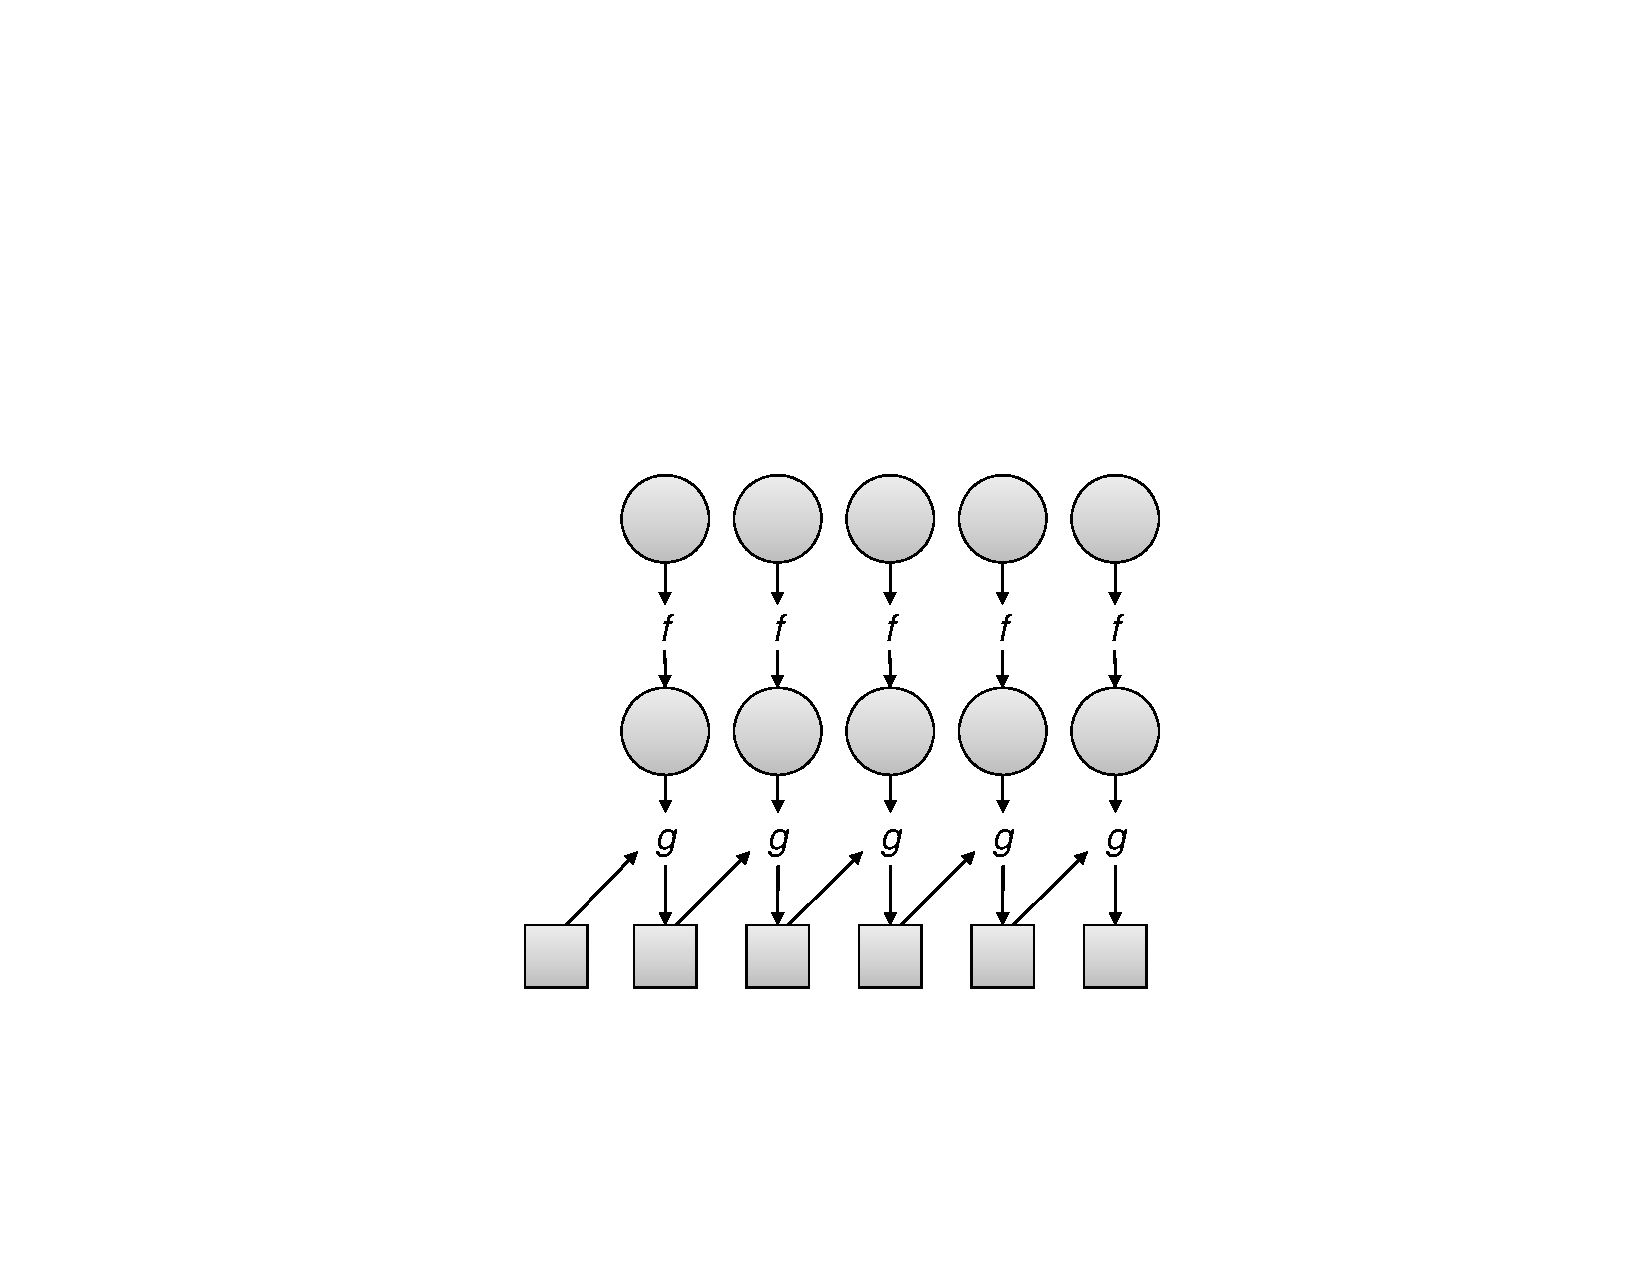
\includegraphics[scale=0.6]{figures/fig-ch2-functional-programming.pdf}
\end{center}
\caption{Illustration of \emph{map} and \emph{fold}, two higher-order
  functions commonly used together in functional programming:\ \emph{
    map} takes a function $f$ and applies it to every element in a
    list, while \emph{fold} iteratively applies a function $g$ to
    aggregate results.}
\label{figure:chapter2:functional}
\end{figure}

We can view \emph{map} as a concise way to represent the transformation
of a dataset (as defined by the function $f$).  In the same vein, we
can view \emph{fold} as an aggregation operation, as defined by the
function $g$.  One immediate observation is that the application of
$f$ to each item in a list (or more generally, to elements in a large
dataset) can be parallelized in a straightforward manner, since each
functional application happens in isolation.  In a cluster, these
operations can be distributed across many different machines.  The
\emph{fold} operation, on the other hand, has more restrictions on data
locality---elements in the list must be ``brought together'' before
the function $g$ can be applied.  However, many real-world
applications do not require $g$ to be applied to \emph{all} elements of
the list.  To the extent that elements in the list can be divided into
groups, the fold aggregations can also proceed in parallel.
Furthermore, for operations that are commutative and associative,
significant efficiencies can be gained in the \emph{fold} operation
through local aggregation and appropriate reordering.

In a nutshell, we have described MapReduce.  The map phase in
MapReduce roughly corresponds to the \emph{map} operation in functional
programming, whereas the reduce phase in MapReduce roughly corresponds
to the \emph{fold} operation in functional programming.  As we will
discuss in detail shortly, the MapReduce execution framework
coordinates the map and reduce phases of processing over large amounts
of data on large clusters of commodity machines.

Viewed from a slightly different angle, MapReduce codifies a generic
``recipe'' for processing large datasets that consists of two stages.
In the first stage, a user-specified computation is applied over all
input records in a dataset.  These operations occur in parallel and
yield intermediate output that is then aggregated by another
user-specified computation.  The programmer defines these two types of
computations, and the execution framework coordinates the actual
processing (very loosely, MapReduce provides a functional
abstraction).  Although such a two-stage processing structure may
appear to be very restrictive, many interesting algorithms can be
expressed quite concisely---especially if one decomposes complex
algorithms into a sequence of MapReduce jobs.  Subsequent chapters in
this book focus on how a number of algorithms can be implemented in
MapReduce.

To be precise, MapReduce can refer to three distinct but related
concepts.  First, MapReduce is a programming model, which is the sense
discussed above.  Second, MapReduce can refer to the execution
framework (i.e., the ``runtime'') that coordinates the execution of
programs written in this particular style.  Finally, MapReduce can
refer to the software implementation of the programming model and the
execution framework:\ for example, Google's proprietary implementation
vs.\ the open-source Hadoop implementation in Java.  And in fact,
there are many implementations of MapReduce, e.g., targeted
specifically for multi-core processors~\cite{Ranger_etal_2007}, for
GPGPUs~\cite{HeB_etal_2008}, for the CELL
architecture~\cite{Rafique_etal_2009}, etc.  There are some
differences between the MapReduce programming model implemented in
Hadoop and Google's proprietary implementation, which we will
explicitly discuss throughout the book.  However, we take a rather
Hadoop-centric view of MapReduce, since Hadoop remains the most mature
and accessible implementation to date, and therefore the one most
developers are likely to use.

\section{Mappers and Reducers}
\label{chapter2:mappers-and-reducers}

Key-value pairs form the basic data structure in MapReduce.  Keys and
values may be primitives such as integers, floating point values,
strings, and raw bytes, or they may be arbitrarily complex structures
(lists, tuples, associative arrays, etc.).  Programmers typically need
to define their own custom data types, although a number of libraries
such as Protocol Buffers,\footnote{\texttt{
https://github.com/google/protobuf}} Thrift,\footnote{\texttt{
http://thrift.apache.org/}} and Avro\footnote{\texttt{
http://avro.apache.org/}} simplify the task.

Part of the design of MapReduce algorithms involves imposing the
key-value structure on arbitrary datasets.  For a collection of web
pages, keys may be URLs and values may be the actual HTML content.
For a graph, keys may represent node ids and values may contain the
adjacency lists of those nodes (see Chapter~\ref{chapter-graphs} for
more details). In some algorithms, input keys are not particularly
meaningful and are simply ignored during processing, while in other
cases input keys are used to uniquely identify a datum (such as a
record id).  In Chapter~\ref{chapter3}, we discuss the role of complex
keys and values in the design of various algorithms.

In MapReduce, the programmer defines a mapper and a reducer with the
following signatures:

\begin{quote}
map: $(k_1, v_1) \rightarrow [(k_2, v_2)]$ \\
reduce: $(k_2, [v_2]) \rightarrow [(k_3, v_3)]$
\end{quote}

\noindent The convention $[\ldots]$ is used
throughout this book to denote a list.  The input to a MapReduce job
starts as data stored on the underlying distributed file system (see
Section~\ref{chapter2:dfs}).  The mapper is applied to every input
key-value pair (split across an arbitrary number of files) to generate
an arbitrary number of intermediate key-value pairs.  The reducer is
applied to all values associated with the same intermediate key to
generate output key-value pairs.\footnote{This characterization, while
conceptually accurate, is a slight simplification.  See
Section~\ref{chapter2:cluster-architecture} for more details.}
Implicit between the map and reduce phases is a distributed ``group
by'' operation on intermediate keys.  Intermediate data arrive at each
reducer in order, sorted by the key.  However, no ordering
relationship is guaranteed for keys across different reducers.  Output
key-value pairs from each reducer are written persistently back onto
the distributed file system (whereas intermediate key-value pairs are
transient and not preserved).  The output ends up in $r$ files on the
distributed file system, where $r$ is the number of reducers.  For the
most part, there is no need to consolidate reducer output, since the
$r$ files often serve as input to yet another MapReduce job.
Figure~\ref{figure:chapter2:MapReduce-simple} illustrates this
two-stage processing structure.
\todo{Rename ``Shuffle and Sort'' to ``Distributed Group By''.}

\begin{figure}
\begin{center}
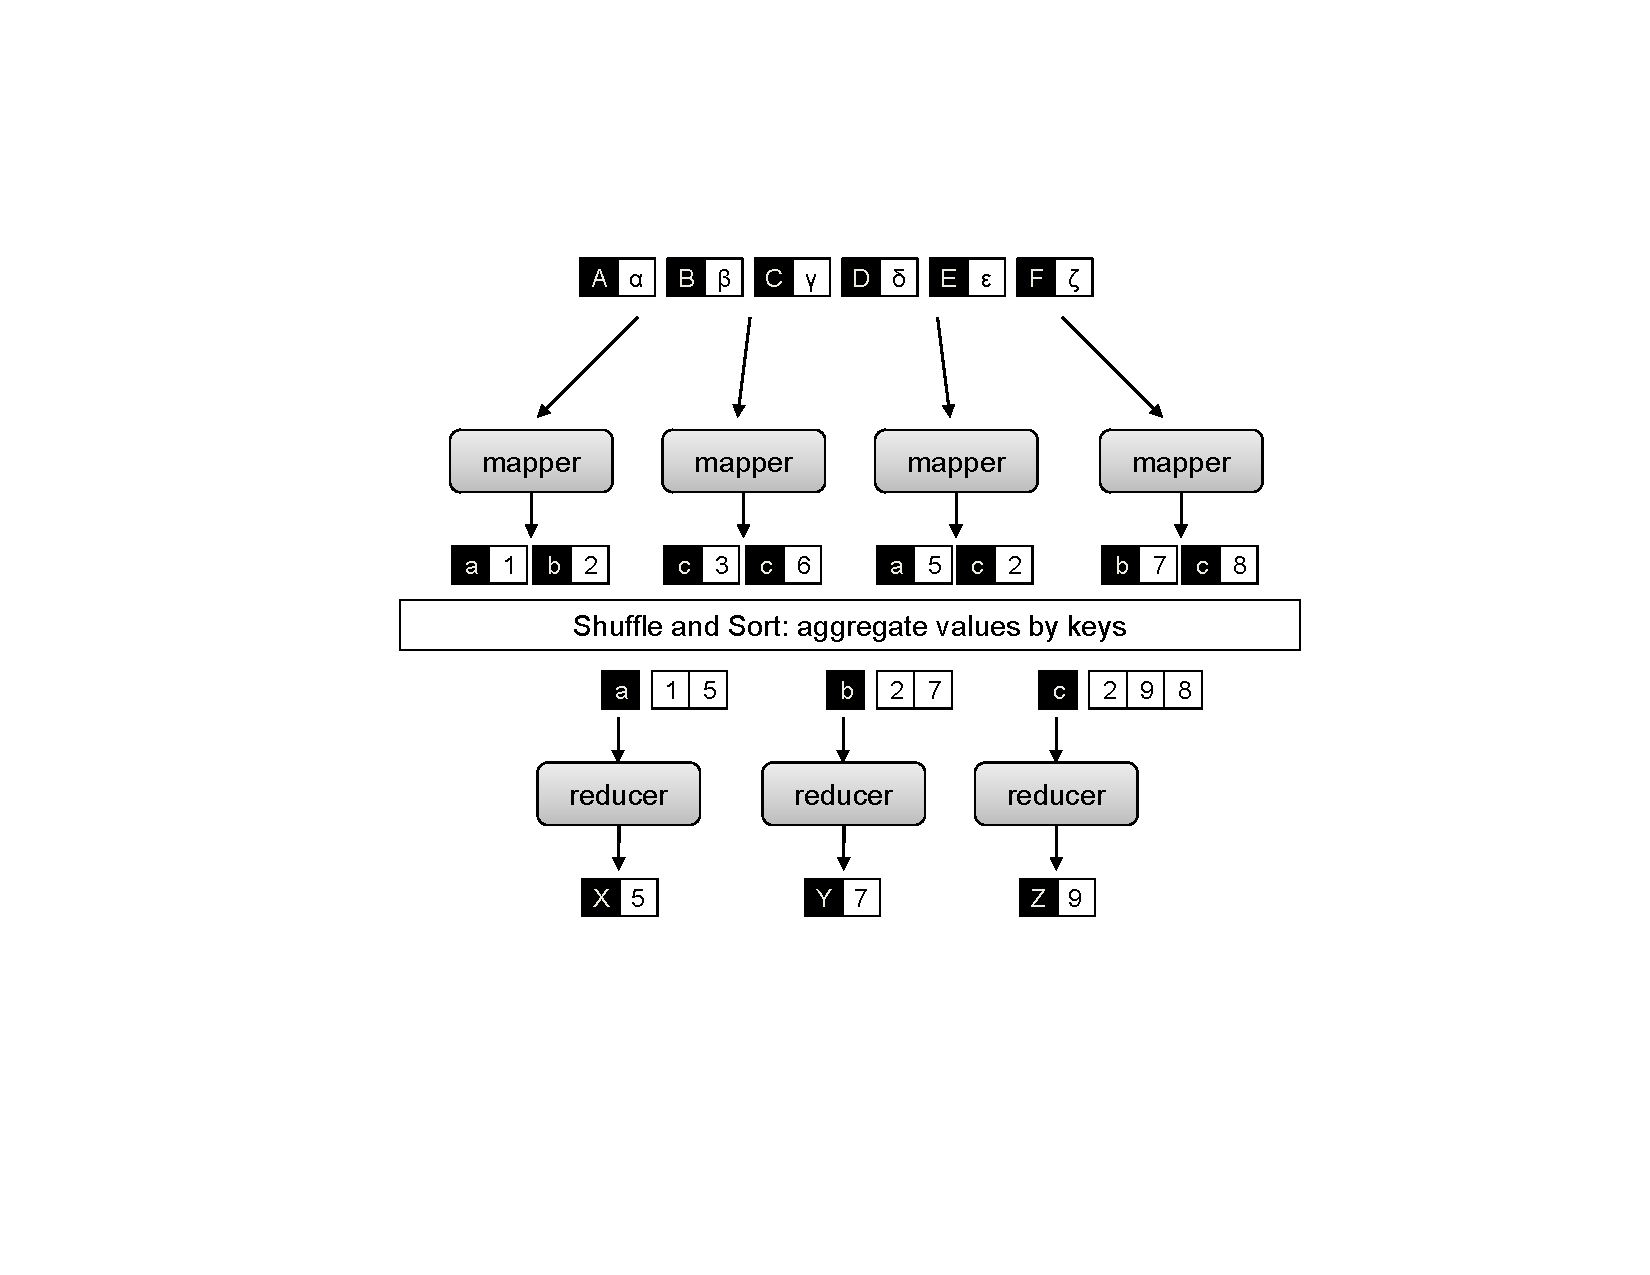
\includegraphics[scale=0.6]{figures/fig-ch2-MapReduce-simple.pdf}
\end{center}
\caption{Simplified view of MapReduce.  Mappers are applied to all
  input key-value pairs, which generate an arbitrary number of
  intermediate key-value pairs.  Reducers are applied to all values
  associated with the same key.  Between the map and reduce phases
  lies a barrier that involves a large distributed sort and group by.}
\label{figure:chapter2:MapReduce-simple}
\end{figure}


\begin{algorithm}[t]
\caption{Word count}
\label{algorithm:chapter2:word-count:basic}
The mapper emits an intermediate key-value pair for each word in an
input document. The reducer sums up all counts for each word.
\begin{small}
\begin{Verbatim}[numbers=left, xleftmargin=7.5mm]
class Mapper {
  def map(key: Long, value: Text) = {
    for (word <- tokenize(value)) {
      emit(word, 1)
  }
}

class Reducer {
  def reduce(key: Text, values: Iterable[Int]) = {
    for (value <- values) {
      sum += value
    }
    emit(key, sum)
  }
}
\end{Verbatim}
\end{small}
\end{algorithm}

A simple word count algorithm in MapReduce is shown in
Algorithm~\ref{algorithm:chapter2:word-count:basic}.  This algorithm counts the
number of occurrences of every word in a text collection, which may be
the first step in, for example, building a unigram language model
(i.e., probability distribution over words in a collection).  Input
key-values pairs take the form of (docid, doc) pairs stored on the
distributed file system, where the former is a unique identifier for
the document, and the latter is the text of the document itself.  The
mapper takes an input key-value pair, tokenizes the document, and
emits an intermediate key-value pair for every word:\ the word itself
serves as the key, and the integer one serves as the value (denoting
that we've seen the word once).  The MapReduce execution framework
guarantees that all values associated with the same key are brought
together in the reducer.  Therefore, in our word count algorithm, we
simply need to sum up all counts (ones) associated with each word.
The reducer does exactly this, and emits final key-value pairs with
the word as the key, and the count as the value.  Final output is
written to the distributed file system, one file per reducer.  Words
within each file will be sorted by alphabetical order, and each file
will contain roughly the same number of words.  The partitioner, which
we discuss later in Section~\ref{chapter2:partitioners-and-combiners},
controls the assignment of words to reducers.  The output can be
examined by the programmer or used as input to another MapReduce
program.

There are some differences between the Hadoop implementation of
MapReduce and Google's implementation.\footnote{Personal
communication, Jeff Dean.}  In Hadoop, the reducer is presented with a
key and an iterator over all values associated with the particular
key.  The values are arbitrarily ordered.  Google's implementation
allows the programmer to specify a secondary sort key for ordering the
values (if desired)---in which case values associated with each key
would be presented to the developer's reduce code in sorted order.
Later in Section~\ref{chapter3:secondary-sorting} we discuss how to
overcome this limitation in Hadoop to perform secondary sorting.
Another difference:\ in Google's implementation the programmer is not
allowed to change the key in the reducer.  That is, the reducer output
key must be exactly the same as the reducer input key.  In Hadoop,
there is no such restriction, and the reducer can emit an arbitrary
number of output key-value pairs (with different keys).

To provide a bit more implementation detail:\ pseudo-code provided in
this book roughly mirrors how MapReduce programs are written in
Hadoop.  Mappers and reducers are objects that implement
the \texttt{map} and \texttt{reduce} methods, respectively.  In
Hadoop, a mapper object is initialized for each map task (associated
with a particular sequence of key-value pairs called an input split)
and the \texttt{map} method is called on each key-value pair by the
execution framework.  In configuring a MapReduce job, the programmer
provides a hint on the number of map tasks to run, but the execution
framework (see next section) makes the final determination based on
the physical layout of the data (more details in
Section~\ref{chapter2:dfs} and
Section~\ref{chapter2:cluster-architecture}).  The situation is
similar for the reduce phase:\ a reducer object is initialized for
each reduce task, and the \texttt{reduce} method is called once per
intermediate key.  In contrast with the number of map tasks, the
programmer can precisely specify the number of reduce tasks.  We will
return to discuss the details of Hadoop job execution in
Section~\ref{chapter2:cluster-architecture}, which is dependent on an
understanding of the distributed file system (covered in
Section~\ref{chapter2:dfs}).  To reiterate:\ although the presentation
of algorithms in this book closely mirrors the way they would be
implemented in Hadoop, our focus is on algorithm design and conceptual
understanding---not actual Hadoop programming.  For that, we would
recommend Tom White's book~\cite{White_2009}.

What are the restrictions on mappers and reducers?  Mappers and
reducers can express arbitrary computations over their inputs.
However, one must generally be careful about use of external resources
since multiple mappers or reducers may be contending for those
resources.  For example, it may be unwise for a mapper to query an
external SQL database, since that would introduce a scalability
bottleneck on the number of map tasks that could be run in parallel
(since they might all be simultaneously querying the
database).\footnote{Unless, of course, the database itself is highly
scalable.} In general, mappers can emit an arbitrary number of
intermediate key-value pairs, and they need not be of the same type as
the input key-value pairs.  Similarly, reducers can emit an arbitrary
number of final key-value pairs, and they can differ in type from the
intermediate key-value pairs.  Although not permitted in functional
programming, mappers and reducers can have side effects.  This is a
powerful and useful feature:\ for example, preserving state across
multiple inputs is central to the design of many MapReduce algorithms
(see Chapter~\ref{chapter3}).  Such algorithms can be understood as
having side effects that only change state that is \emph{internal} to
the mapper or reducer.  While the correctness of such algorithms may
be more difficult to guarantee (since the function's behavior depends
not only on the current input but on previous inputs), most potential
synchronization problems are avoided since internal state is private
only to individual mappers and reducers.  In other cases (see
Section~\ref{chapter-indexing:index:revised} and
Section~\ref{chapter6_variants}), it may be useful for mappers or
reducers to have \emph{external} side effects, such as writing files
to the distributed file system.  Since many mappers and reducers are
run in parallel, and the distributed file system is a shared global
resource, special care must be taken to ensure that such operations
avoid synchronization conflicts.  One strategy is to write a temporary
file that is renamed upon successful completion of the mapper or
reducer~\cite{Dean_Ghemawat_OSDI2004}.

In addition to the ``canonical'' MapReduce processing flow, other
variations are also possible.  MapReduce programs can contain no
reducers, in which case mapper output is directly written to disk (one
file per mapper).  For embarrassingly parallel problems, e.g., parse a
large text collection or independently analyze a large number of
images, this would be a common pattern.  The converse---a MapReduce
program with no mappers---is not possible, although in some cases it
is useful for the mapper to implement the identity function and simply
pass input key-value pairs to the reducers.  This has the effect of
sorting and regrouping the input for reduce-side processing.
Similarly, in some cases it is useful for the reducer to implement the
identity function, in which case the program simply sorts and groups
mapper output.  Finally, running identity mappers and reducers has the
effect of regrouping and resorting the input data (which is sometimes
useful).

Although in the most common case, input to a MapReduce job comes from
data stored on the distributed file system and output is written back
to the distributed file system, any other system that satisfies the
proper abstractions can serve as a data source or sink.  With Google's
MapReduce implementation, BigTable~\cite{ChangFay_etal_OSDI2006}, a
sparse, distributed, persistent multidimensional sorted map, is
frequently used as a source of input and as a store of MapReduce
output.  HBase is an open-source BigTable clone and has similar
capabilities.  Also, Hadoop has been integrated with existing MPP
(massively parallel processing) relational databases, which allows a
programmer to write MapReduce jobs over database rows and dump output
into a new database table.  Finally, in some cases MapReduce jobs may
not consume any input at all (e.g., computing $\pi$) or may only
consume a small amount of data (e.g., input parameters to many
instances of processor-intensive simulations running in parallel).

\section{The Execution Framework}
\label{chapter2:execution-framework}

One of the most important idea behind MapReduce is separating the \emph{
what} of distributed processing from the \emph{how}.  A MapReduce
program, referred to as a job, consists of code for mappers and
reducers (as well as combiners and partitioners to be discussed in the
next section) packaged together with configuration parameters (such as
where the input lies and where the output should be stored).  The
developer submits the job to the submission node of a cluster (in
Hadoop, this is called the jobtracker) and execution framework
(sometimes called the ``runtime'') takes care of everything else:\ it
transparently handles all other aspects of distributed code execution,
on clusters ranging from a single node to a few thousand nodes.
Specific responsibilities include:

\paragraph{Scheduling.} Each MapReduce job is divided into smaller
units called tasks (see Section~\ref{chapter2:cluster-architecture}
for more details).  For example, a map task may be responsible for
processing a certain block of input key-value pairs (called an input
split in Hadoop); similarly, a reduce task may handle a portion of the
intermediate key space.  It is not uncommon for MapReduce jobs to have
thousands of individual tasks that need to be assigned to nodes in the
cluster.  In large jobs, the total number of tasks may exceed the
number of tasks that can be run on the cluster concurrently, making it
necessary for the scheduler to maintain some sort of a task queue and
to track the progress of running tasks so that waiting tasks can be
assigned to nodes as they become available.  Another aspect of
scheduling involves coordination among tasks belonging to different
jobs (e.g., from different users).  How can a large, shared resource
support several users simultaneously in a predictable, transparent,
policy-driven fashion?  There has been some recent work along these
lines in the context of
Hadoop~\cite{Sandholm_Lai_2009,Zaharia_etal_2009}.

Speculative execution is an optimization implemented by both
Hadoop and Google's MapReduce implementation (called ``backup
tasks''~\cite{Dean_Ghemawat_OSDI2004}).  Due to the barrier between
the map and reduce tasks, the map phase of a job is only as fast as
the slowest map task.  Similarly, the completion time of a job is
bounded by the running time of the slowest reduce task.  As a result,
the speed of a MapReduce job is sensitive to what are known as \emph{
stragglers}, or tasks that take an usually long time to complete.  One
cause of stragglers is flaky hardware:\ for example, a machine that is
suffering from recoverable errors may become significantly slower.
With speculative execution, an identical copy of the same task is
executed on a different machine, and the framework simply uses the
result of the first task attempt to finish.  Zaharia et
al.~\cite{Zaharia_etal_OSDI2008} presented different execution
strategies in a recent paper, and Google has reported that speculative
execution can improve job running times by
44\%~\cite{Dean_Ghemawat_OSDI2004}.  Although in Hadoop both map and
reduce tasks can be speculatively executed, the common wisdom is that
the technique is more helpful for map tasks than reduce tasks, since
each copy of the reduce task needs to pull data over the network.
Note, however, that speculative execution cannot adequately address
another common cause of stragglers:\ skew in the distribution of
values associated with intermediate keys (leading to reduce
stragglers).  In text processing we often observe Zipfian
distributions, which means that the task or tasks responsible for
processing the most frequent few elements will run much longer than
the typical task.  Better local aggregation, discussed in the next
chapter, is one possible solution to this problem.

\paragraph{Data/code co-location.}  The phrase \emph{data
  distribution} is misleading, since one of the key ideas behind
MapReduce is to move the code, not the data.  However, the more
general point remains---in order for computation to occur, we need to
somehow feed data to the code.  In MapReduce, this issue is
inextricably intertwined with scheduling and relies heavily on the
design of the underlying distributed file system.\footnote{In the
canonical case, that is.  Recall that MapReduce may receive its input
from other sources.} To achieve data locality, the scheduler starts
tasks on the node that holds a particular block of data (i.e., on its
local drive) needed by the task.  This has the effect of moving code
to the data.  If this is not possible (e.g., a node is already running
too many tasks), new tasks will be started elsewhere, and the
necessary data will be streamed over the network.  An important
optimization here is to prefer nodes that are on the same rack in the
datacenter as the node holding the relevant data block, since
inter-rack bandwidth is significantly less than intra-rack bandwidth.

\paragraph{Synchronization.} In general, synchronization refers to
the mechanisms by which multiple concurrently running processes ``join
up'', for example, to share intermediate results or otherwise exchange
state information.  In MapReduce, synchronization is accomplished by a
barrier between the map and reduce phases of processing.  Intermediate
key-value pairs must be grouped by key, which is accomplished by a
large distributed sort involving all the nodes that executed map tasks
and all the nodes that will execute reduce tasks.  This necessarily
involves copying intermediate data over the network, and therefore the
process is commonly known as ``shuffle and sort''.  A MapReduce job
with $m$ mappers and $r$ reducers involves up to $m \times r$ distinct
copy operations, since each mapper may have intermediate output going
to every reducer.

Note that the reduce computation cannot start until all the mappers
have finished emitting key-value pairs and all intermediate key-value
pairs have been shuffled and sorted, since the execution framework
cannot otherwise guarantee that all values associated with the same
key have been gathered.  This is an important departure from
functional programming:\ in a \emph{fold} operation, the aggregation
function $g$ is a function of the intermediate value and the next item
in the list---which means that values can be lazily generated and
aggregation can begin as soon as values are available.  In contrast,
the reducer in MapReduce receives \emph{all} values associated with the
same key at once.  However, it is possible to start copying
intermediate key-value pairs over the network to the nodes running the
reducers as soon as each mapper finishes---this is a common
optimization and implemented in Hadoop.

\paragraph{Error and fault handling.}  The MapReduce execution
framework must accomplish all the tasks above in an environment where
errors and faults are the norm, not the exception.  Since MapReduce
was explicitly designed around low-end commodity servers, the runtime
must be especially resilient.  In large clusters, disk failures are
common~\cite{Pinheiro_etal_2007} and RAM experiences more errors than
one might expect~\cite{Schroeder_etal_2009}.  Datacenters suffer from
both planned outages (e.g., system maintenance and hardware upgrades)
and unexpected outages (e.g., power failure, connectivity loss, etc.).

And that's just hardware.  No software is bug free---exceptions must
be appropriately trapped, logged, and recovered from.  Large-data
problems have a penchant for uncovering obscure corner cases in code
that is otherwise thought to be bug-free.  Furthermore, any
sufficiently large dataset will contain corrupted data or records that
are mangled beyond a programmer's imagination---resulting in errors
that one would never think to check for or trap.  The MapReduce
execution framework must thrive in this hostile environment.

\section{Partitioners and Combiners}
\label{chapter2:partitioners-and-combiners}

We have thus far presented a simplified view of MapReduce.  There are
two additional elements that complete the programming model:\
partitioners and combiners.

Partitioners are responsible for dividing up the intermediate key
space and assigning intermediate key-value pairs to reducers.  In
other words, the partitioner specifies the task to which an
intermediate key-value pair must be copied.  Within each reducer, keys
are processed in sorted order (which is how the ``group by'' is
implemented).  The simplest partitioner involves computing the hash
value of the key and then taking the mod of that value with the number
of reducers.  This assigns approximately the same number of keys to
each reducer (dependent on the quality of the hash function).  Note,
however, that the partitioner only considers the key and ignores the
value---therefore, a roughly-even partitioning of the key space may
nevertheless yield large differences in the number of key-values pairs
sent to each reducer (since different keys may have different numbers
of associated values).  This imbalance in the amount of data
associated with each key is relatively common in many text processing
applications due to the Zipfian distribution of word occurrences.

Combiners are an optimization in MapReduce that allow for local
aggregation before the shuffle and sort phase.  We can motivate the
need for combiners by considering the word count algorithm in
Algorithm~\ref{algorithm:chapter2:word-count:basic}, which emits a key-value pair
for each word in the collection.  Furthermore, all these key-value
pairs need to be copied across the network, and so the amount of
intermediate data will be larger than the input collection itself.
This is clearly inefficient.  One solution is to perform local
aggregation on the output of each mapper, i.e., to compute a local
count for a word over all the documents processed by the mapper.  With
this modification (assuming the maximum amount of local aggregation
possible), the number of intermediate key-value pairs will be at most
the number of unique words in the collection times the number of
mappers (and typically far smaller because each mapper may not
encounter every word).

The combiner in MapReduce supports such an optimization.  One can
think of combiners as ``mini-reducers'' that take place on the output
of the mappers, prior to the shuffle and sort phase.  Each combiner
operates in isolation and therefore does not have access to
intermediate output from other mappers.  The combiner is provided keys
and values associated with each key (the same types as the mapper
output keys and values).  Critically, one cannot assume that a
combiner will have the opportunity to process \emph{all} values
associated with the same key.  The combiner can emit any number of
key-value pairs, but the keys and values must be of the same type as
the mapper output (same as the reducer input).\footnote{A note on the
implementation of combiners in Hadoop:\ by default, the execution
framework reserves the right to use combiners at its discretion.  In
reality, this means that a combiner may be invoked zero, one, or
multiple times.  In addition, combiners in Hadoop may actually be
invoked in the reduce phase, i.e., after key-value pairs have been
copied over to the reducer, but before the user reducer code runs.  As
a result, combiners must be carefully written so that they can be
executed in these different environments.
Section~\ref{chapter3:local-aggregation:correctness} discusses this in
more detail.}  In cases where an operation is both associative and
commutative (e.g., addition or multiplication), reducers can directly
serve as combiners.  In general, however, reducers and combiners are
not interchangeable.

In many cases, proper use of combiners can spell the difference
between an impractical algorithm and an efficient algorithm.  This
topic will be discussed in Section~\ref{chapter3:local-aggregation},
which focuses on various techniques for local aggregation.  It
suffices to say for now that a combiner can significantly reduce the
amount of data that needs to be copied over the network, resulting in
much faster algorithms.

The complete MapReduce model is shown in
Figure~\ref{figure:chapter2:MapReduce-complete}.  Output of the
mappers are processed by the combiners, which perform local
aggregation to cut down on the number of intermediate key-value pairs.
The partitioner determines which reducer will be responsible for
processing a particular key, and the execution framework uses this
information to copy the data to the right location during the shuffle
and sort phase.\footnote{In Hadoop, partitioners are actually executed
before combiners, so while
Figure~\ref{figure:chapter2:MapReduce-complete} is conceptually
accurate, it doesn't precisely describe the Hadoop implementation.}
Therefore, a complete MapReduce job consists of code for the mapper,
reducer, combiner, and partitioner, along with job configuration
parameters.  The execution framework handles everything else.

\begin{figure}[t]
\begin{center}
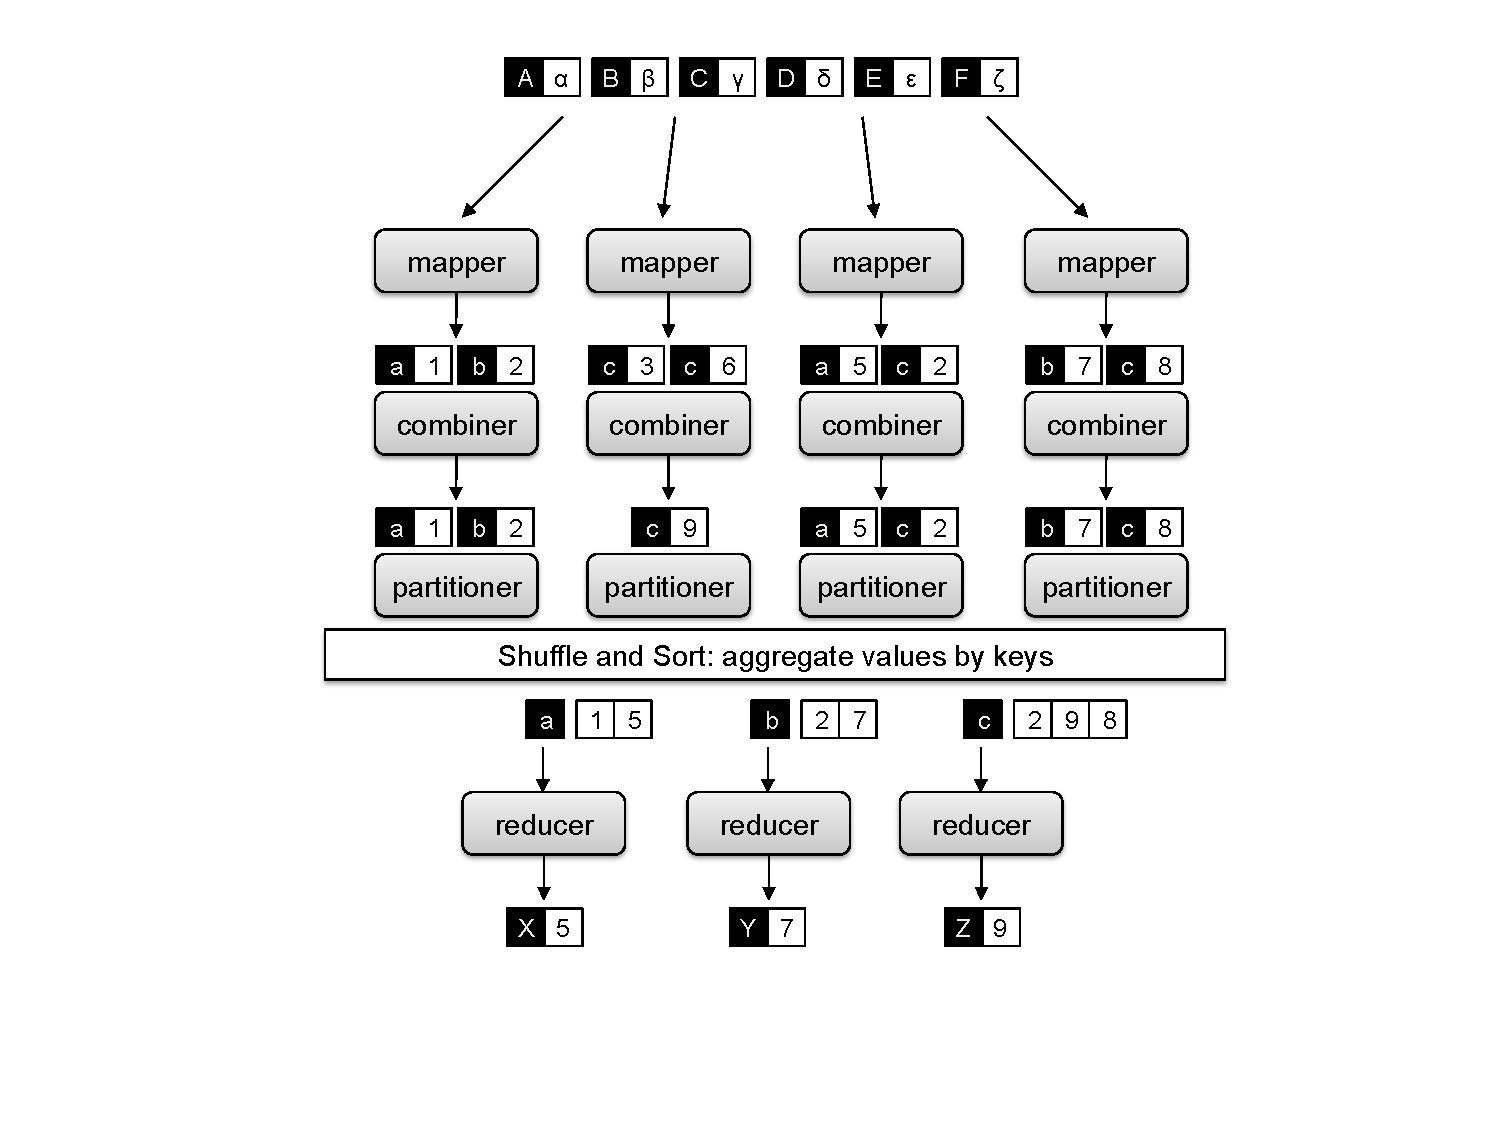
\includegraphics[scale=0.6]{figures/fig-ch2-MapReduce-complete.pdf}
\end{center}
\caption{Complete view of MapReduce, illustrating combiners and
  partitioners in addition to mappers and reducers.  Combiners can be
  viewed as ``mini-reducers'' in the map phase.  Partitioners
  determine which reducer is responsible for a particular key.}
\label{figure:chapter2:MapReduce-complete}
\end{figure}

\section{The Distributed File System}
\label{chapter2:dfs}

So far, we have mostly focused on the \emph{processing} aspect of
data-intensive processing, but it is important to recognize that
without data, there is nothing to compute on.  In high-performance
computing (HPC) and many traditional cluster architectures, storage is
viewed as a distinct and separate component from computation.
Implementations vary widely, but network-attached storage (NAS) and
storage area networks (SAN) are common; supercomputers often have
dedicated subsystems for handling storage (separate nodes, and often
even separate networks).  Regardless of the details, the processing
cycle remains the same at a high level:\ the compute nodes fetch input
from storage, load the data into memory, process the data, and then
write back the results (with perhaps intermediate checkpointing for
long-running processes).

As dataset sizes increase, more compute capacity is required for
processing.  But as compute capacity grows, the link between the
compute nodes and the storage becomes a bottleneck.  At that point,
one could invest in higher performance but more expensive networks
(e.g., 10 gigabit Ethernet) or special-purpose interconnects such as
InfiniBand (even more expensive).  In most cases, this is not a
cost-effective solution, as the price of networking equipment
increases non-linearly with performance (e.g., a switch with ten times
the capacity is usually more than ten times more expensive).
Alternatively, one could abandon the separation of computation and
storage as distinct components in a cluster.  The distributed file
system (DFS) that underlies MapReduce adopts exactly this approach.
The Google File System (GFS)~\cite{Ghemawat_etal_SOSP2003} supports
Google's proprietary implementation of MapReduce; in the open-source
world, HDFS (Hadoop Distributed File System) is an open-source
implementation of GFS that supports Hadoop.  Although MapReduce
doesn't necessarily require the distributed file system, it is
difficult to realize many of the advantages of the programming model
without a storage substrate that behaves much like the
DFS.\footnote{However, there is evidence that existing POSIX-based
distributed cluster file systems (e.g., GPFS or PVFS) can serve as a
replacement for HDFS, when properly tuned or modified for MapReduce
workloads~\cite{Tantisiriroj_etal_2008,Ananthanarayanan_etal_2009}.
This, however, remains an experimental use case.}

Of course, distributed file systems are not
new~\cite{Howard_etal_1988,Cabrera_Long_1991,Anderson_etal_SOSP1995,Thekkath_etal_SOSP1997,Schmuck_Haskin_2002}.
The MapReduce distributed file system builds on previous work but is
specifically adapted to large-data processing workloads, and therefore
departs from previous architectures in certain respects (see
discussion by Ghemawat et al.~\cite{Ghemawat_etal_SOSP2003} in the
original GFS paper.).  The main idea is to divide user data into
blocks and replicate those blocks across the local disks of nodes in
the cluster.  Blocking data, of course, is not a new idea, but DFS
blocks are significantly larger than block sizes in typical
single-machine file systems (64 MB by default).  The distributed file
system adopts a master--slave architecture in which the master
maintains the file namespace (metadata, directory structure, file to
block mapping, location of blocks, and access permissions) and the
slaves manage the actual data blocks.  In GFS, the master is called
the GFS master, and the slaves are called GFS chunkservers.  In
Hadoop, the same roles are filled by the namenode and datanodes,
respectively.\footnote{To be precise, namenode and datanode may refer
to physical machines in a cluster, or they may refer to daemons
running on those machines providing the relevant services.} This book
adopts the Hadoop terminology, although for most basic file operations
GFS and HDFS work much the same way.  The architecture of HDFS is
shown in Figure~\ref{figure:chapter2:HDFS}, redrawn from a similar
diagram describing GFS~\cite{Ghemawat_etal_SOSP2003}.

\begin{figure}[t]
\begin{center}
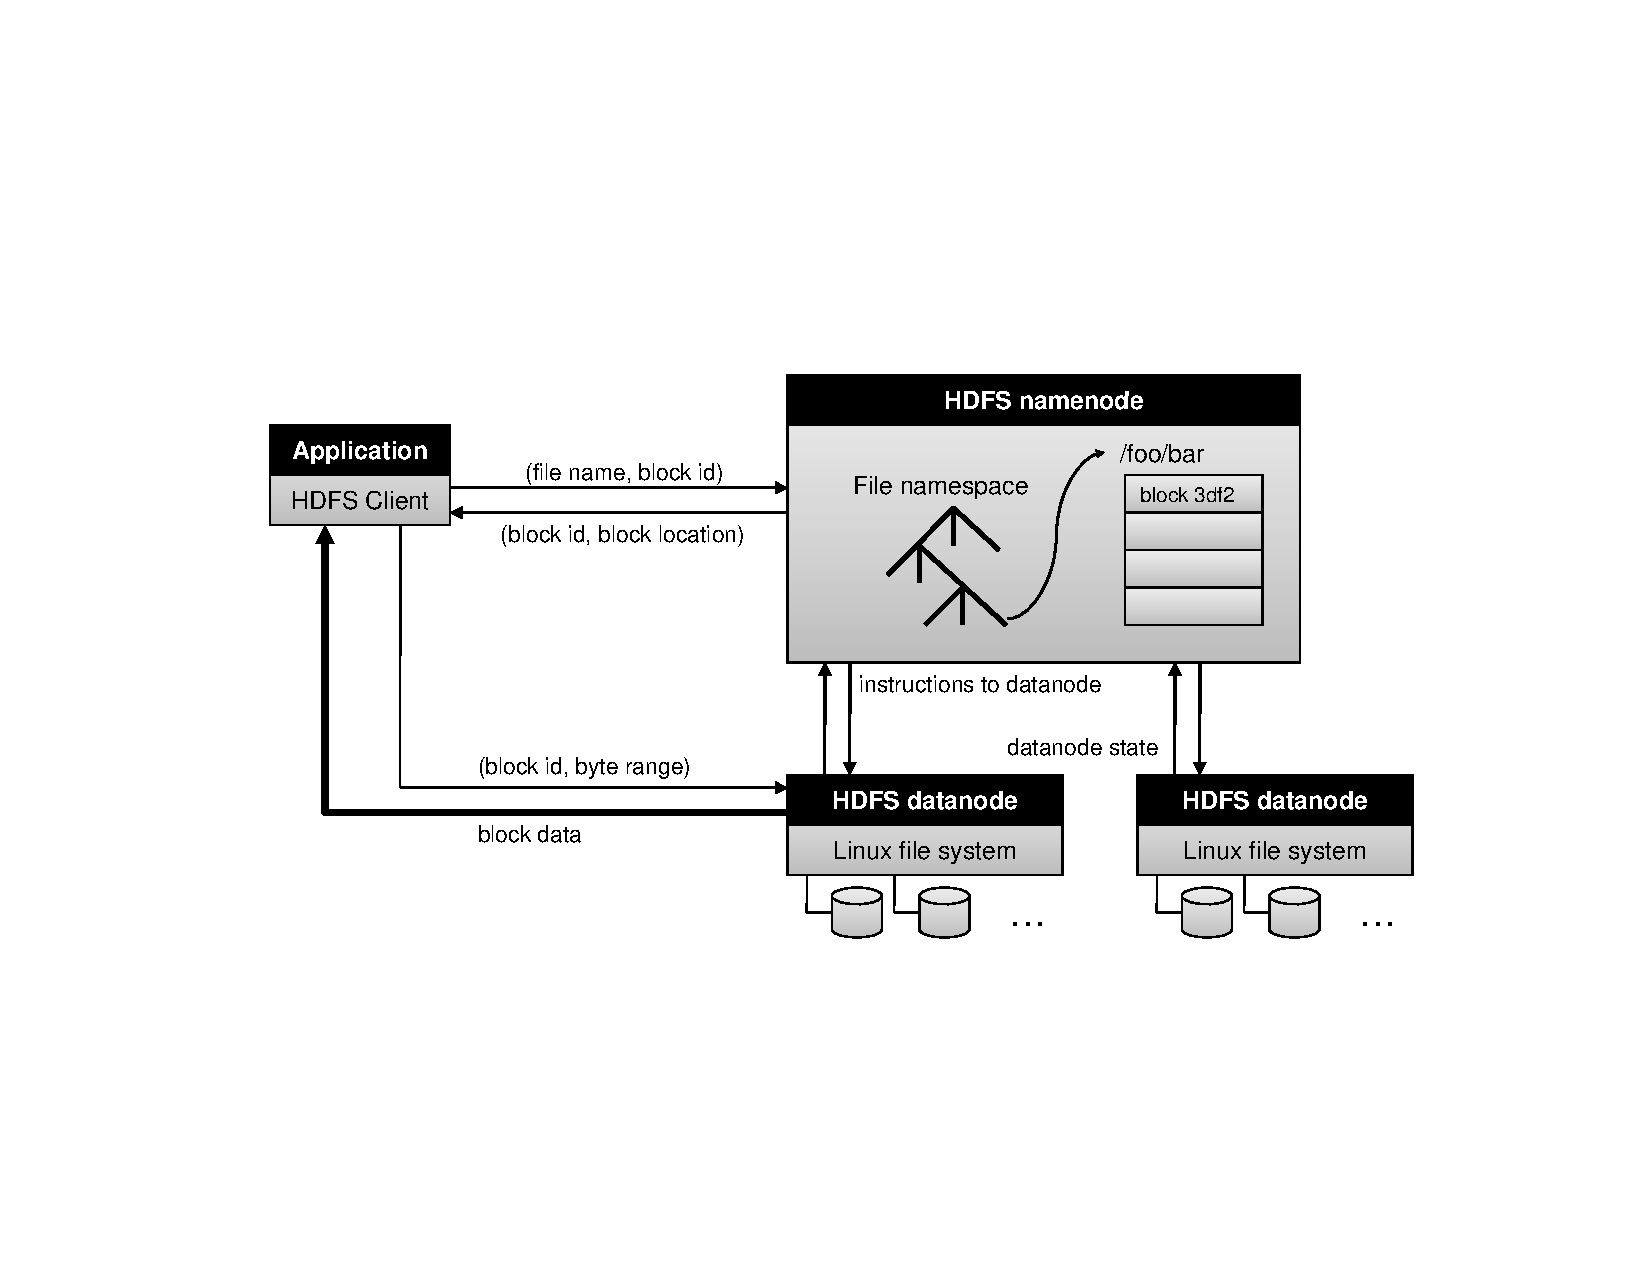
\includegraphics[scale=0.6]{figures/fig-ch2-HDFS.pdf}
\end{center}
\caption{The architecture of HDFS.  The namenode (master) is responsible for maintaining the file
  namespace and directing clients to datanodes (slaves) that actually
  hold data blocks containing user data.}
\label{figure:chapter2:HDFS}
\end{figure}

In HDFS, an application client wishing to read a file (or a portion
thereof) must first contact the namenode to determine where the actual
data is stored.  In response to the client request, the namenode
returns the relevant block id and the location where the block is held
(i.e., which datanode).  The client then contacts the datanode to
retrieve the data.  Blocks are themselves stored on standard
single-machine file systems, so HDFS lies on top of the standard OS
stack (e.g., Linux).  An important feature of the design is that data
is never moved through the namenode.  Instead, all data transfer
occurs directly between clients and datanodes; communications with the
namenode only involves transfer of metadata.

By default, HDFS stores three separate copies of each data block to
ensure both reliability, availability, and performance.  In large
clusters, the three replicas are spread across different physical
racks, so HDFS is resilient towards two common failure scenarios:\
individual datanode crashes and failures in networking equipment that
bring an entire rack offline.  Replicating blocks across physical
machines also increases opportunities to co-locate data and processing
in the scheduling of MapReduce jobs, since multiple copies yield more
opportunities to exploit locality.  The namenode is in periodic
communication with the datanodes to ensure proper replication of all
the blocks:\ if there aren't enough replicas (e.g., due to disk or
machine failures or to connectivity losses due to networking equipment
failures), the namenode directs the creation of additional
copies;\footnote{Note that the namenode coordinates the replication
process, but data transfer occurs directly from datanode to datanode.}
if there are too many replicas (e.g., a repaired node rejoins the
cluster), extra copies are discarded.

To create a new file and write data to HDFS, the application client
first contacts the namenode, which updates the file namespace after
checking permissions and making sure the file doesn't already exist.
The namenode allocates a new block on a suitable datanode, and the
application is directed to stream data directly to it.  From the
initial datanode, data is further propagated to additional replicas.
In the most recent release of Hadoop as of this writing (release
0.20.2), files are immutable---they cannot be modified after creation.
There are current plans to officially support file appends in the near
future, which is a feature already present in GFS.

In summary, the HDFS namenode has the following responsibilities:

\begin{itemize}

\item Namespace management.  The namenode is responsible for
  maintaining the file namespace, which includes metadata, directory
  structure, file to block mapping, location of blocks, and access
  permissions.  These data are held in memory for fast access and all
  mutations are persistently logged.

\item Coordinating file operations.  The namenode directs application
  clients to datanodes for read operations, and allocates blocks on
  suitable datanodes for write operations.  All data transfers occur
  directly between clients and datanodes.  When a file is deleted,
  HDFS does not immediately reclaim the available physical storage;
  rather, blocks are lazily garbage collected.

\item Maintaining overall health of the file system. The namenode is
  in periodic contact with the datanodes via heartbeat messages to
  ensure the integrity of the system.  If the namenode observes that a
  data block is under-replicated (fewer copies are stored on datanodes
  than the desired replication factor), it will direct the creation of
  new replicas.  Finally, the namenode is also responsible for
  rebalancing the file system.\footnote{In Hadoop, this is a
  manually-invoked process.}  During the course of normal operations,
  certain datanodes may end up holding more blocks than others;
  rebalancing involves moving blocks from datanodes with more blocks
  to datanodes with fewer blocks.  This leads to better load balancing
  and more even disk utilization.

\end{itemize}

\noindent Since GFS and HDFS were specifically designed to support
Google's proprietary and the open-source implementation of MapReduce,
respectively, they were designed with a number of assumptions about
the operational environment, which in turn influenced the design of
the systems.  Understanding these choices is critical to designing
effective MapReduce algorithms:

\begin{itemize}

\item The file system stores a relatively modest number of large
  files.  The definition of ``modest'' varies by the size of the
  deployment, but in HDFS multi-gigabyte files are common (and even
  encouraged).  There are several reasons why lots of small files are
  to be avoided.  Since the namenode must hold all file metadata in
  memory, this presents an upper bound on both the number of files and
  blocks that can be supported.\footnote{According to Dhruba Borthakur
  in a post to the Hadoop mailing list on 6/8/2008, each block in HDFS
  occupies about 150 bytes of memory on the namenode.} Large
  multi-block files represent a more efficient use of namenode memory
  than many single-block files (each of which consumes less space than
  a single block size).  In addition, mappers in a MapReduce job use
  individual files as a basic unit for splitting input data.  At
  present, there is no default mechanism in Hadoop that allows a
  mapper to process multiple files.  As a result, mapping over many
  small files will yield as many map tasks as there are files.  This
  results in two potential problems:\ first, the startup costs of
  mappers may become significant compared to the time spent actually
  processing input key-value pairs; second, this may result in an
  excessive amount of across-the-network copy operations during the
  ``shuffle and sort'' phase (recall that a MapReduce job with $m$
  mappers and $r$ reducers involves up to $m \times r$ distinct copy
  operations).

\item Workloads are batch oriented, dominated by long streaming
  reads and large sequential writes.  As a result, high sustained
  bandwidth is more important than low latency.  This exactly
  describes the nature of MapReduce jobs, which are batch operations
  on large amounts of data.  Due to the common-case workload, both
  HDFS and GFS do not implement any form of data
  caching.\footnote{However, since the distributed file system is
  built on top of a standard operating system such as Linux, there is
  still OS-level caching.}

\item Applications are aware of the characteristics of the distributed
  file system.  Neither HDFS nor GFS present a general POSIX-compliant
  API, but rather support only a subset of possible file operations.
  This simplifies the design of the distributed file system, and in
  essence pushes part of the data management onto the end application.
  One rationale for this decision is that each application knows best
  how to handle data specific to that application, for example, in
  terms of resolving inconsistent states and optimizing the layout of
  data structures.

\item The file system is deployed in an environment of cooperative
  users.  There is no discussion of security in the original GFS
  paper, but HDFS explicitly assumes a datacenter environment where
  only authorized users have access.  File permissions in HDFS are
  only meant to prevent unintended operations and can be easily
  circumvented.\footnote{However, there are existing plans to
  integrate Kerberos into Hadoop/HDFS.}

\item The system is built from unreliable but inexpensive commodity
  components.  As a result, failures are the norm rather than the
  exception.  HDFS is designed around a number of self-monitoring and
  self-healing mechanisms to robustly cope with common failure modes.

\end{itemize}

\noindent Finally, some discussion is necessary to understand the
single-master design of HDFS and GFS.  It has been demonstrated that
in large-scale distributed systems, simultaneously providing
consistency, availability, and partition tolerance is
impossible---this is Brewer's so-called CAP
Theorem~\cite{Gilbert_Lynch_2002}.  Since partitioning is unavoidable
in large-data systems, the real tradeoff is between consistency and
availability.  A single-master design trades availability for
consistency and significantly simplifies implementation.  If the
master (HDFS namenode or GFS master) goes down, the entire file system
becomes unavailable, which trivially guarantees that the file system
will never be in an inconsistent state.  An alternative design might
involve multiple masters that jointly manage the file namespace---such
an architecture would increase availability (if one goes down, another
can step in) at the cost of consistency, not to mention requiring a
more complex implementation
(cf.~\cite{Alvaro_etal_2009,McKusick_Quinlan_2009}).

The single-master design of GFS and HDFS is a well-known weakness,
since if the master goes offline, the entire file system and all
MapReduce jobs running on top of it will grind to a halt.  This
weakness is mitigated in part by the lightweight nature of file system
operations.  Recall that no data is ever moved through the namenode
and that all communication between clients and datanodes involve only
metadata.  Because of this, the namenode rarely is the bottleneck, and
for the most part avoids load-induced crashes.  In practice, this
single point of failure is not as severe a limitation as it may
appear---with diligent monitoring of the namenode, mean time between
failure measured in months are not uncommon for production
deployments.  Furthermore, the Hadoop community is well-aware of this
problem and has developed several reasonable workarounds---for
example, a warm standby namenode that can be quickly switched over
when the primary namenode fails.  The open source environment and the
fact that many organizations already depend on Hadoop for production
systems virtually guarantees that more effective solutions will be
developed over time.

\section{Hadoop Cluster Architecture}
\label{chapter2:cluster-architecture}

Putting everything together, the architecture of a complete Hadoop
cluster is shown in Figure~\ref{figure:chapter2:Hadoop-cluster}.  The
HDFS namenode runs the namenode daemon.  The job submission node runs
the jobtracker, which is the single point of contact for a client
wishing to execute a MapReduce job.  The jobtracker monitors the
progress of running MapReduce jobs and is responsible for coordinating
the execution of the mappers and reducers.  Typically, these services
run on two separate machines, although in smaller clusters they are
often co-located.  The bulk of a Hadoop cluster consists of slave
nodes (only three of which are shown in the figure) that run both a
tasktracker, which is responsible for actually running user code, and
a datanode daemon, for serving HDFS data.

\begin{figure}[t]
\begin{center}
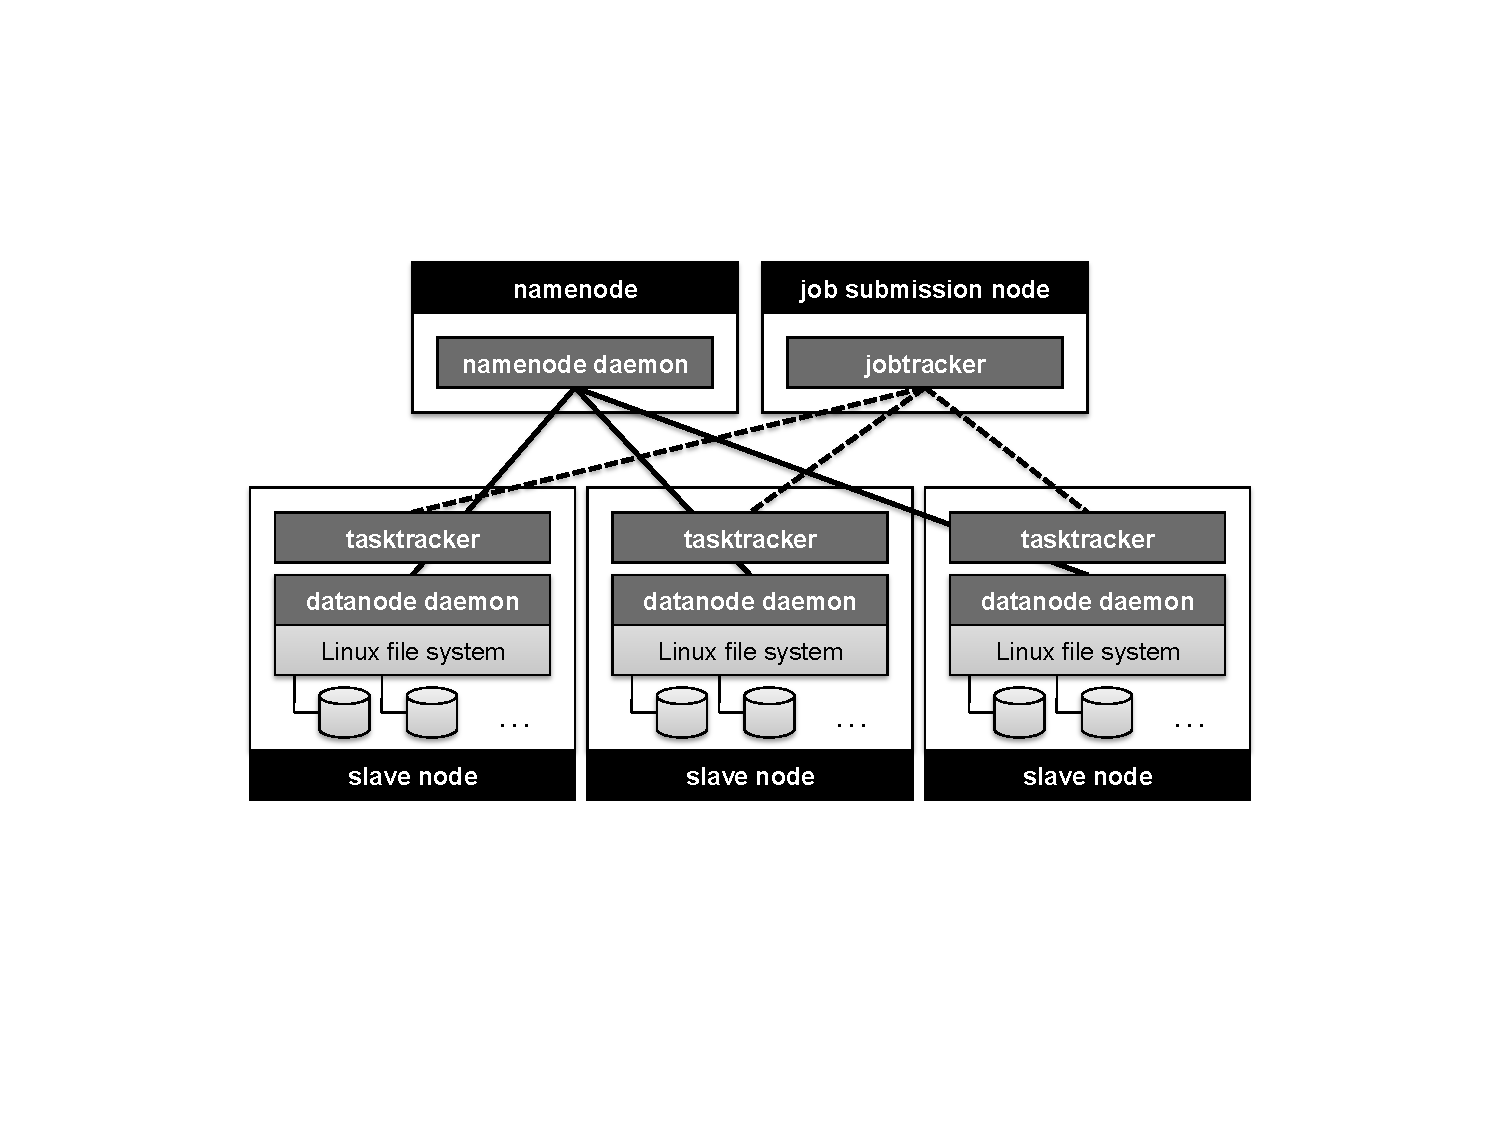
\includegraphics[scale=0.6]{figures/fig-ch2-Hadoop.pdf}
\end{center}
\caption{Architecture of a complete Hadoop cluster, which consists of
  three separate components:\ the HDFS master (called the namenode),
  the job submission node (called the jobtracker), and many slave
  nodes (three shown here).  Each of the slave nodes runs a
  tasktracker for executing map and reduce tasks and a datanode daemon
  for serving HDFS data.}
\label{figure:chapter2:Hadoop-cluster}
\end{figure}

A Hadoop MapReduce job is divided up into a number of map tasks and
reduce tasks.  Tasktrackers periodically send heartbeat messages to
the jobtracker that also doubles as a vehicle for task allocation.  If
a tasktracker is available to run tasks (in Hadoop parlance, has empty
task slots), the return acknowledgment of the tasktracker heartbeat
contains task allocation information.  The number of reduce tasks is
equal to the number of reducers specified by the programmer.  The
number of map tasks, on the other hand, depends on many factors:\ the
number of mappers specified by the programmer serves as a hint to the
execution framework, but the actual number of tasks depends on both
the number of input files and the number of HDFS data blocks occupied
by those files.  Each map task is assigned a sequence of input
key-value pairs, called an input split in Hadoop.  Input splits are
computed automatically and the execution framework strives to align
them to HDFS block boundaries so that each map task is associated with
a single data block.  In scheduling map tasks, the jobtracker tries to
take advantage of data locality---if possible, map tasks are scheduled
on the slave node that holds the input split, so that the mapper will
be processing local data.  The alignment of input splits with HDFS
block boundaries simplifies task scheduling.  If it is not possible to
run a map task on local data, it becomes necessary to stream input
key-value pairs across the network.  Since large clusters are
organized into racks, with far greater intra-rack bandwidth than
inter-rack bandwidth, the execution framework strives to at least
place map tasks on a rack which has a copy of the data block.

Although conceptually in MapReduce one can think of the mapper being
applied to all input key-value pairs and the reducer being applied to
all values associated with the same key, actual job execution is a bit
more complex.  In Hadoop, mappers are Java objects with a \texttt{map}
method (among others).  A mapper object is instantiated for every map
task by the tasktracker.  The life-cycle of this object begins with
instantiation, where a hook is provided in the API to run
programmer-specified code.  This means that mappers can read in ``side
data'', providing an opportunity to load state, static data sources,
dictionaries, etc.  After initialization, the \texttt{map} method is
called (by the execution framework) on all key-value pairs in the
input split.  Since these method calls occur in the context of the
same Java object, it is possible to preserve state across multiple
input key-value pairs within the same map task---this is an important
property to exploit in the design of MapReduce algorithms, as we will
see in the next chapter.  After all key-value pairs in the input split
have been processed, the mapper object provides an opportunity to run
programmer-specified termination code.  This, too, will be important
in the design of MapReduce algorithms.

The actual execution of reducers is similar to that of the mappers.
Each reducer object is instantiated for every reduce task.  The Hadoop
API provides hooks for programmer-specified initialization and
termination code.  After initialization, for each intermediate key in
the partition (defined by the partitioner), the execution framework
repeatedly calls the \texttt{reduce} method with an intermediate key
and an iterator over all values associated with that key.  The
programming model also guarantees that intermediate keys will be
presented to the \texttt{reduce} method in sorted order.  Since this
occurs in the context of a single object, it is possible to preserve
state across multiple intermediate keys (and associated values) within
a single reduce task.  Once again, this property is critical in the
design of MapReduce algorithms and will be discussed in the next
chapter.

\section{Summary}
\label{chapter2:summary}

This chapter provides a basic overview of the MapReduce programming
model, starting with its roots in functional programming and
continuing with a description of mappers, reducers, partitioners, and
combiners.  Significant attention is also given to the underlying
distributed file system, which is a tightly-integrated component of
the MapReduce environment.  Given this basic understanding, we now
turn our attention to the design of MapReduce algorithms.

\chapter{MapReduce Algorithm Design}
\label{chapter3}

A large part of the power of MapReduce comes from its simplicity:\ in
addition to preparing the input data, the programmer needs only to
implement the mapper, the reducer, and optionally, the combiner and
the partitioner.  All other aspects of execution are handled
transparently by the execution framework---on clusters ranging from a
single node to a few thousand nodes, over datasets ranging from
gigabytes to petabytes.  However, this also means that any conceivable
algorithm that a programmer wishes to develop must be expressed in
terms of a small number of rigidly-defined components that must fit
together in very specific ways.  It may not appear obvious how a
multitude of algorithms can be recast into this programming model.
The purpose of this chapter is to provide, primarily through examples,
a guide to MapReduce algorithm design.  These examples illustrate what
can be thought of as ``design patterns'' for MapReduce, which
instantiate arrangements of components and specific techniques
designed to handle frequently-encountered situations across a variety
of problem domains.  Two of these design patterns are used in the
scalable inverted indexing algorithm we'll present later in
Chapter~\ref{chapter-indexing}; concepts presented here will show up
again in Chapter~\ref{chapter-graphs} (graph processing) and
Chapter~\ref{chapter6} (expectation-maximization algorithms).

Synchronization is perhaps the most tricky aspect of designing
MapReduce algorithms (or for that matter, parallel and distributed
algorithms in general).  Other than embarrassingly-parallel problems,
processes running on separate nodes in a cluster must, at some point
in time, come together---for example, to distribute partial results
from nodes that produced them to the nodes that will consume them.
Within a single MapReduce job, there is only one opportunity for
cluster-wide synchronization---during the shuffle and sort stage where
intermediate key-value pairs are copied from the mappers to the
reducers and grouped by key.  Beyond that, mappers and reducers run in
isolation without any mechanisms for direct communication.
Furthermore, the programmer has little control over many aspects of
execution, for example:

\begin{itemize}

\item {\it Where} a mapper or reducer runs (i.e., on which node in the
  cluster).

\item {\it When} a mapper or reducer begins or finishes.

\item {\it Which} input key-value pairs are processed by a specific
  mapper.

\item {\it Which} intermediate key-value pairs are processed by a
  specific reducer.

\end{itemize}

\noindent Nevertheless, the programmer does have a number of
techniques for controlling execution and managing the flow of data in
MapReduce.  In summary, they are:

\begin{enumerate}

\item The ability to construct complex data structures as keys and
  values to store and communicate partial results.

\item The ability to execute user-specified initialization code at the
  beginning of a map or reduce task, and the ability to execute
  user-specified termination code at the end of a map or reduce task.

\item The ability to preserve state in both mappers and reducers
  across multiple input or intermediate keys.

\item The ability to control the sort order of intermediate keys, and
  therefore the order in which a reducer will encounter particular
  keys.

\item The ability to control the partitioning of the key space, and
  therefore the set of keys that will be encountered by a particular
  reducer.

\end{enumerate}

\noindent It is important to realize that many algorithms cannot be
easily expressed as a single MapReduce job.  One must often decompose
complex algorithms into a sequence of jobs, which requires
orchestrating data so that the output of one job becomes the input to
the next.  Many algorithms are iterative in nature, requiring repeated
execution until some convergence criteria---graph algorithms in
Chapter~\ref{chapter-graphs} and expectation-maximization algorithms
in Chapter~\ref{chapter6} behave in exactly this way.  Often, the
convergence check itself cannot be easily expressed in MapReduce.  The
standard solution is an external (non-MapReduce) program that serves
as a ``driver'' to coordinate MapReduce iterations.

This chapter explains how various techniques to control code execution
and data flow can be applied to design algorithms in MapReduce.  The
focus is both on scalability---ensuring that there are no inherent
bottlenecks as algorithms are applied to increasingly larger
datasets---and efficiency---ensuring that algorithms do not needlessly
consume resources and thereby reducing the cost of parallelization.
The gold standard, of course, is linear scalability:\ an algorithm
running on twice the amount of data should take only twice as long.
Similarly, an algorithm running on twice the number of nodes should
only take half as long.  

The chapter is organized as follows:

\begin{itemize}

\item Section~\ref{chapter3:local-aggregation} introduces the
  important concept of local aggregation in MapReduce and strategies
  for designing efficient algorithms that minimize the amount of
  partial results that need to be copied across the network.  The
  proper use of combiners is discussed in detail, as well as the
  ``in-mapper combining'' design pattern.

\item Section~\ref{chapter3:pairs-and-stripes} uses the example of
  building word co-occurrence matrices on large text corpora to
  illustrate two common design patterns, which we dub ``pairs'' and
  ``stripes''.  These two approaches are useful in a large class of
  problems that require keeping track of joint events across a large
  number of observations.

\item Section~\ref{chapter3:cond-prob} shows how co-occurrence counts
  can be converted into relative frequencies using a pattern known as
  ``order inversion''.  The sequencing of computations in the reducer
  can be recast as a sorting problem, where pieces of intermediate
  data are sorted into exactly the order that is required to carry out
  a series of computations.  Often, a reducer needs to compute an
  aggregate statistic on a set of elements before individual elements
  can be processed.  Normally, this would require two passes over the
  data, but with the ``order inversion'' design pattern, the aggregate
  statistic can be computed in the reducer before the individual
  elements are encountered.  This may seem counter-intuitive:\ how can
  we compute an aggregate statistic on a set of elements before
  encountering elements of that set?  As it turns out, clever sorting
  of special key-value pairs enables exactly this.

\item Section~\ref{chapter3:secondary-sorting} provides a general
  solution to secondary sorting, which is the problem of sorting
  values associated with a key in the reduce phase.  We call this
  technique ``value-to-key conversion''.

\item Section~\ref{chapter3:joins} covers the topic of performing
  joins on relational datasets and presents three different
  approaches:\ {\it reduce-side}, {\it map-side}, and {\it
    memory-backed} joins.

\end{itemize}

\section{Local Aggregation}
\label{chapter3:local-aggregation}

In the context of data-intensive distributed processing, the single
most important aspect of synchronization is the exchange of
intermediate results, from the processes that produced them to the
processes that will ultimately consume them.  In a cluster
environment, with the exception of embarrassingly-parallel problems,
this necessarily involves transferring data over the network.
Furthermore, in Hadoop, intermediate results are written to local disk
before being sent over the network.  Since network and disk latencies
are relatively expensive compared to other operations, reductions in
the amount of intermediate data translate into increases in
algorithmic efficiency.  In MapReduce, local aggregation of
intermediate results is one of the keys to efficient algorithms.
Through use of the combiner and by taking advantage of the ability to
preserve state across multiple inputs, it is often possible to
substantially reduce both the number and size of key-value pairs that
need to be shuffled from the mappers to the reducers.

\subsection{Combiners and In-Mapper Combining}
\label{chapter3:local-aggregation:combiners}

We illustrate various techniques for local aggregation using the
simple word count example presented in
Section~\ref{chapter2:mappers-and-reducers}.  For convenience,
Figure~\ref{figure:chapter3:word-count:basic} repeats the pseudo-code
of the basic algorithm, which is quite simple:\ the mapper emits an
intermediate key-value pair for each term observed, with the term
itself as the key and a value of one; reducers sum up the partial
counts to arrive at the final count.

The first technique for local aggregation is the combiner, already
discussed in Section~\ref{chapter2:partitioners-and-combiners}.
Combiners provide a general mechanism within the MapReduce framework
to reduce the amount of intermediate data generated by the
mappers---recall that they can be understood as ``mini-reducers'' that
process the output of mappers.  In this example, the combiners
aggregate term counts across the documents processed by each map task.
This results in a reduction in the number of intermediate key-value
pairs that need to be shuffled across the network---from the order of
{\it total} number of terms in the collection to the order of the
number of {\it unique} terms in the collection.\footnote{More
  precisely, if the combiners take advantage of all opportunities for
  local aggregation, the algorithm would generate at most $m \times V$
  intermediate key-value pairs, where $m$ is the number of mappers and
  $V$ is the vocabulary size (number of unique terms in the
  collection), since every term could have been observed in every
  mapper.  However, there are two additional factors to consider.  Due
  to the Zipfian nature of term distributions, most terms will not be
  observed by most mappers (for example, terms that occur only once
  will by definition only be observed by one mapper).  On the other
  hand, combiners in Hadoop are treated as {\it optional}
  optimizations, so there is no guarantee that the execution framework
  will take advantage of all opportunities for partial aggregation.}

\begin{figure}[t]
\algrenewcommand\algorithmicfunction{\textbf{class}}
\algrenewcommand\algorithmicprocedure{\textbf{method}}
  \begin{algorithmic}[1]
    \Function{Mapper}{}
    \Procedure{Map}{$\textrm{docid }a, \textrm{doc }d$}
    \ForAll{$\textrm{term }t \in \textrm{doc }d$}
    \State $\textsc{Emit}(\textrm{term }t, \textrm{count }1)$
    \EndFor
    \EndProcedure
    \EndFunction
  \end{algorithmic}

  \begin{algorithmic}[1]
    \Function{Reducer}{}
    \Procedure{Reduce}{$\textrm{term }t, \textrm{counts }[  c_1, c_2, \ldots ]$}
    \State $sum \gets 0$
    \ForAll{$ \textrm{count }c \in \textrm{counts }[  c_1, c_2, \ldots ]$}
    \State $sum \gets sum + c$
    \EndFor
    \State $\textsc{Emit}(\textrm{term }t, \textrm{count }sum)$
    \EndProcedure
    \EndFunction
  \end{algorithmic}
  \caption{Pseudo-code for the basic word count algorithm in MapReduce
    (repeated from Figure~\ref{chapter2:word-count:basic}).}
\label{figure:chapter3:word-count:basic}
\end{figure}

An improvement on the basic algorithm is shown in
Figure~\ref{figure:chapter3:word-count:inner-hash} (the mapper is
modified but the reducer remains the same as in
Figure~\ref{figure:chapter3:word-count:basic} and therefore is not
repeated).  An associative array (i.e., Map in Java) is introduced
inside the mapper to tally up term counts within a single
document:\ instead of emitting a key-value pair for each term in the
document, this version emits a key-value pair for each {\it unique}
term in the document.  Given that some words appear frequently within
a document (for example, a document about dogs is likely to have many
occurrences of the word ``dog''), this can yield substantial savings
in the number of intermediate key-value pairs emitted, especially for
long documents.

\begin{figure}[t]
\algrenewcommand\algorithmicfunction{\textbf{class}}
\algrenewcommand\algorithmicprocedure{\textbf{method}}
  \begin{algorithmic}[1]
    \Function{Mapper}{}
    \Procedure{Map}{$\textrm{docid }a, \textrm{doc }d$}
    \State $H \gets \textrm{new }\textsc{AssociativeArray}$
    \ForAll{$\textrm{term }t \in \textrm{doc }d$}
      \State $H\{t\} \gets H\{t\} + 1$\Comment{Tally counts for entire document}
    \EndFor
    \ForAll{$\textrm{term }t \in H$}
    \State $\textsc{Emit}(\textrm{term }t, \textrm{count }H\{t\} )$
    \EndFor
    \EndProcedure
    \EndFunction
  \end{algorithmic}
  \caption{Pseudo-code for the improved MapReduce word count algorithm
    that uses an associative array to aggregate term counts on a
    per-document basis.  Reducer is the same as in
    Figure~\ref{figure:chapter3:word-count:basic}.}
\label{figure:chapter3:word-count:inner-hash}
\end{figure}

This basic idea can be taken one step further, as illustrated in the
variant of the word count algorithm in
Figure~\ref{figure:chapter3:word-count:outer-hash} (once again, only
the mapper is modified).  The workings of this algorithm critically
depends on the details of how map and reduce tasks in Hadoop are
executed, discussed in Section~\ref{chapter2:cluster-architecture}.
Recall, a (Java) mapper object is created for each map task, which is
responsible for processing a block of input key-value pairs.  Prior to
processing any input key-value pairs, the mapper's \textsc{Initialize}
method is called, which is an API hook for user-specified code.  In
this case, we initialize an associative array for holding term counts.
Since it is possible to preserve state across multiple calls of the
\textsc{Map} method (for each input key-value pair), we can continue
to accumulate partial term counts in the associative array {\it
  across} multiple documents, and emit key-value pairs only when the
mapper has processed all documents.  That is, emission of intermediate
data is deferred until the \textsc{Close} method in the pseudo-code.
Recall that this API hook provides an opportunity to execute
user-specified code {\it after} the \textsc{Map} method has been
applied to all input key-value pairs of the input data split to which
the map task was assigned.

\begin{figure}[t]
\algrenewcommand\algorithmicfunction{\textbf{class}}
\algrenewcommand\algorithmicprocedure{\textbf{method}}
  \begin{algorithmic}[1]
    \Function{Mapper}{}
    \Procedure{Initialize}{}
    \State $H \gets \textrm{new }\textsc{AssociativeArray}$
    \EndProcedure
    \Procedure{Map}{$\textrm{docid }a, \textrm{doc }d$}
    \ForAll{$\textrm{term }t \in \textrm{doc }d$}
    \State $H\{t\} \gets H\{t\} + 1$\Comment{Tally counts {\it across} documents}
    \EndFor
    \EndProcedure
    \Procedure{Close}{}
    \ForAll{$\textrm{term }t \in H$}
    \State $\textsc{Emit}(\textrm{term }t, \textrm{count }H\{t\} )$
    \EndFor
    \EndProcedure
    \EndFunction
  \end{algorithmic}
  \caption{Pseudo-code for the improved MapReduce word count algorithm
    that demonstrates the ``in-mapper combining'' design pattern.
    Reducer is the same as in
    Figure~\ref{figure:chapter3:word-count:basic}.}
\label{figure:chapter3:word-count:outer-hash}
\end{figure}

With this technique, we are in essence incorporating combiner
functionality directly inside the mapper.  There is no need to run a
separate combiner, since all opportunities for local aggregation are
already exploited.\footnote{Leaving aside the minor complication that
  in Hadoop, combiners can be run in the reduce phase also (when
  merging intermediate key-value pairs from different map tasks).
  However, in practice it makes almost no difference either way.} This
is a sufficiently common design pattern in MapReduce that it's worth
giving it a name, ``in-mapper combining'', so that we can refer to the
pattern more conveniently throughout the book.  We'll see later on how
this pattern can be applied to a variety of problems.  There are two
main advantages to using this design pattern:

First, it provides control over when local aggregation occurs and how
it exactly takes place.  In contrast, the semantics of the combiner is
underspecified in MapReduce.  For example, Hadoop makes no guarantees
on how many times the combiner is applied, or that it is even applied
at all.  The combiner is provided as a semantics-preserving
optimization to the execution framework, which has the {\it option} of
using it, perhaps multiple times, or not at all (or even in the reduce
phase).  In some cases (although not in this particular example), such
indeterminism is unacceptable, which is exactly why programmers often
choose to perform their own local aggregation in the mappers.

Second, in-mapper combining will typically be more efficient than
using actual combiners.  One reason for this is the additional
overhead associated with actually materializing the key-value pairs.
Combiners reduce the amount of intermediate data that is shuffled
across the network, but don't actually reduce the number of key-value
pairs that are emitted by the mappers in the first place.  With the
algorithm in Figure~\ref{figure:chapter3:word-count:inner-hash},
intermediate key-value pairs are still generated on a per-document
basis, only to be ``compacted'' by the combiners.  This process
involves unnecessary object creation and destruction (garbage
collection takes time), and furthermore, object serialization and
deserialization (when intermediate key-value pairs fill the in-memory
buffer holding map outputs and need to be temporarily spilled to
disk). In contrast, with in-mapper combining, the mappers will
generate only those key-value pairs that need to be shuffled across
the network to the reducers.

There are, however, drawbacks to the in-mapper combining pattern.
First, it breaks the functional programming underpinnings of
MapReduce, since state is being preserved across multiple input
key-value pairs.  Ultimately, this isn't a big deal, since pragmatic
concerns for efficiency often trump theoretical ``purity'', but there
are practical consequences as well.  Preserving state across multiple
input instances means that algorithmic behavior may depend on the
order in which input key-value pairs are encountered.  This creates
the potential for ordering-dependent bugs, which are difficult to
debug on large datasets in the general case (although the correctness
of in-mapper combining for word count is easy to demonstrate).
Second, there is a fundamental scalability bottleneck associated with
the in-mapper combining pattern.  It critically depends on having
sufficient memory to store intermediate results until the mapper has
completely processed all key-value pairs in an input split.  In the
word count example, the memory footprint is bound by the vocabulary
size, since it is theoretically possible that a mapper encounters
every term in the collection.  Heap's Law, a well-known result in
information retrieval, accurately models the growth of vocabulary size
as a function of the collection size---the somewhat surprising fact is
that the vocabulary size never stops growing.\footnote{In more detail,
  Heap's Law relates the vocabulary size $V$ to the collection size as
  follows:\ $V =kT^b$, where $T$ is the number of tokens in the
  collection.  Typical values of the parameters $k$ and $b$ are:\ $30
  \leq k \leq 100$ and $b \sim 0.5$~(\cite{Manning_etal_2008},
  p.\ 81).}  Therefore, the algorithm in
Figure~\ref{figure:chapter3:word-count:outer-hash} will scale only up
to a point, beyond which the associative array holding the partial
term counts will no longer fit in memory.\footnote{A few more
  details:\ note what matters is that the partial term counts
  encountered within particular {\it input split} fits into memory.
  However, as collection sizes increase, one will often want to
  increase the input split size to limit the growth of the number of
  map tasks (in order to reduce the number of distinct copy operations
  necessary to shuffle intermediate data over the network).}

One common solution to limiting memory usage when using the in-mapper
combining technique is to ``block'' input key-value pairs and
``flush'' in-memory data structures periodically.  The idea is
simple:\ instead of emitting intermediate data only after {\it every}
key-value pair has been processed, emit partial results after
processing every $n$ key-value pairs.  This is straightforwardly
implemented with a counter variable that keeps track of the number of
input key-value pairs that have been processed.  As an alternative,
the mapper could keep track of its own memory footprint and flush
intermediate key-value pairs once memory usage has crossed a certain
threshold.  In both approaches, either the block size or the memory
usage threshold needs to be determined empirically:\ with too large a
value, the mapper may run out of memory, but with too small a value,
opportunities for local aggregation may be lost.  Furthermore, in
Hadoop physical memory is split between multiple tasks that may be
running on a node concurrently; these tasks are all competing for
finite resources, but since the tasks are not aware of each other, it
is difficult to coordinate resource consumption effectively.  In
practice, however, one often encounters diminishing returns in
performance gains with increasing buffer sizes, such that it is not
worth the effort to search for an {\it optimal} buffer size (personal
communication, Jeff Dean).

In MapReduce algorithms, the extent to which efficiency can be
increased through local aggregation depends on the size of the
intermediate key space, the distribution of keys themselves, and the
number of key-value pairs that are emitted by each individual map
task.  Opportunities for aggregation, after all, come from having
multiple values associated with the same key (whether one uses
combiners or employs the in-mapper combining pattern).  In the word
count example, local aggregation is effective because many words are
encountered multiple times within a map task.  Local aggregation is
also an effective technique for dealing with reduce stragglers (see
Section~\ref{chapter2:execution-framework}) that result from a
highly-skewed (e.g., Zipfian) distribution of values associated with
intermediate keys.  In our word count example, we do not filter
frequently-occurring words:\ therefore, without local aggregation, the
reducer that's responsible for computing the count of `the' will
have a lot more work to do than the typical reducer, and therefore
will likely be a straggler.  With local aggregation (either combiners
or in-mapper combining), we substantially reduce the number of values
associated with frequently-occurring terms, which alleviates the
reduce straggler problem.

\subsection{Algorithmic Correctness with Local Aggregation}
\label{chapter3:local-aggregation:correctness}

Although use of combiners can yield dramatic reductions in algorithm
running time, care must be taken in applying them.  Since combiners in
Hadoop are viewed as optional optimizations, the correctness of the
algorithm cannot depend on computations performed by the combiner or
depend on them even being run at all.  In any MapReduce program, the
reducer input key-value type must match the mapper output key-value
type:\ this implies that the combiner input {\it and} output key-value
types must match the mapper output key-value type (which is the same
as the reducer input key-value type).  In cases where the reduce
computation is both commutative and associative, the reducer can also
be used (unmodified) as the combiner (as is the case with the word
count example).  In the general case, however, combiners and reducers
are not interchangeable.

Consider a simple example:\ we have a large dataset where input keys
are strings and input values are integers, and we wish to compute the
mean of all integers associated with the same key (rounded to the
nearest integer).  A real-world example might be a large user log from
a popular website, where keys represent user ids and values represent
some measure of activity such as elapsed time for a particular
session---the task would correspond to computing the mean session
length on a per-user basis, which would be useful for understanding
user demographics.  Figure~\ref{figure:chapter3:average} shows the
pseudo-code of a simple algorithm for accomplishing this task that
does not involve combiners.  We use an identity mapper, which simply
passes all input key-value pairs to the reducers (appropriately
grouped and sorted).  The reducer keeps track of the running sum and
the number of integers encountered.  This information is used to
compute the mean once all values are processed.  The mean is then
emitted as the output value in the reducer (with the input string as
the key).

\begin{figure}[t]
\algrenewcommand\algorithmicfunction{\textbf{class}}
\algrenewcommand\algorithmicprocedure{\textbf{method}}
  \begin{algorithmic}[1]
    \Function{Mapper}{}
    \Procedure{Map}{$\textrm{string }t, \textrm{integer }r$}
    \State $\textsc{Emit}(\textrm{string }t, \textrm{integer }r)$
    \EndProcedure
    \EndFunction
  \end{algorithmic}

  \begin{algorithmic}[1]
    \Function{Reducer}{}
    \Procedure{Reduce}{$\textrm{string }t, \textrm{integers }[ r_1, r_2, \ldots ]$}
    \State $sum \gets 0$
    \State $cnt \gets 0$
    \ForAll{$ \textrm{integer }r \in \textrm{integers }[ r_1, r_2, \ldots ]$}
    \State $sum \gets sum + r$
    \State $cnt \gets cnt + 1$
    \EndFor
    \State $r_{avg} \gets sum/cnt$
    \State $\textsc{Emit}(\textrm{string }t, \textrm{integer } r_{avg})$
    \EndProcedure
    \EndFunction
  \end{algorithmic}
  \caption{Pseudo-code for the basic MapReduce algorithm that computes
    the mean of values associated with the same key.}
\label{figure:chapter3:average}
\end{figure}

This algorithm will indeed work, but suffers from the same drawbacks
as the basic word count algorithm in
Figure~\ref{figure:chapter3:word-count:basic}:\ it requires shuffling
all key-value pairs from mappers to reducers across the network, which
is highly inefficient.  Unlike in the word count example, the reducer
cannot be used as a combiner in this case.  Consider what would happen
if we did:\ the combiner would compute the mean of an arbitrary subset
of values associated with the same key, and the reducer would compute
the mean of those values.  As a concrete example, we know that:

\begin{equation}
\textsc{Mean}(1, 2, 3, 4, 5) \ne \textsc{Mean}( \textsc{Mean}(1, 2), \textsc{Mean}(3, 4, 5))
\end{equation}

\noindent In general, the mean of means of arbitrary subsets of a set
of numbers is not the same as the mean of the set of numbers.
Therefore, this approach would not produce the correct
result.\footnote{There is, however, one special case in which using
  reducers as combiners {\it would} produce the correct result:\ if
  each combiner computed the mean of equal-size subsets of the values.
  However, since such fine-grained control over the combiners is
  impossible in MapReduce, such a scenario is highly unlikely.}

So how might we properly take advantage of combiners?  An attempt is
shown in Figure~\ref{figure:chapter3:average-fail}.  The mapper
remains the same, but we have added a combiner that partially
aggregates results by computing the numeric components necessary to
arrive at the mean.  The combiner receives each string and the
associated list of integer values, from which it computes the sum of
those values and the number of integers encountered (i.e., the count).
The sum and count are packaged into a pair, and emitted as the output
of the combiner, with the same string as the key.  In the reducer,
pairs of partial sums and counts can be aggregated to arrive at the
mean.  Up until now, all keys and values in our algorithms have been
primitives (string, integers, etc.).  However, there are no
prohibitions in MapReduce for more complex types,\footnote{In Hadoop,
  either custom types or types defined using a library such as
  Protocol Buffers, Thrift, or Avro.} and, in fact, this represents a
key technique in MapReduce algorithm design that we introduced at the
beginning of this chapter.  We will frequently encounter complex keys
and values throughput the rest of this book.

\begin{figure}[t]
\algrenewcommand\algorithmicfunction{\textbf{class}}
\algrenewcommand\algorithmicprocedure{\textbf{method}}
  \begin{algorithmic}[1]
    \Function{Mapper}{}
    \Procedure{Map}{$\textrm{string }t, \textrm{integer }r$}
    \State $\textsc{Emit}(\textrm{string }t, \textrm{integer }r)$
    \EndProcedure
    \EndFunction
  \end{algorithmic}

  \begin{algorithmic}[1]
    \Function{Combiner}{}
    \Procedure{Combine}{$\textrm{string }t, \textrm{integers }[ r_1, r_2, \ldots ]$}
    \State $sum \gets 0$
    \State $cnt \gets 0$
    \ForAll{$ \textrm{integer }r \in \textrm{integers }[ r_1, r_2, \ldots ]$}
    \State $sum \gets sum + r$
    \State $cnt \gets cnt + 1$
    \EndFor
    \State $\textsc{Emit}(\textrm{string }t, \textrm{pair } (sum, cnt))$\Comment{Separate sum and count}
    \EndProcedure
    \EndFunction
  \end{algorithmic}

  \begin{algorithmic}[1]
    \Function{Reducer}{}
    \Procedure{Reduce}{$\textrm{string }t, \textrm{pairs }[ (s_1, c_1), (s_2, c_2) \ldots ]$}
    \State $sum \gets 0$
    \State $cnt \gets 0$
    \ForAll{$ \textrm{pair }(s, c) \in \textrm{pairs }[ (s_1, c_1), (s_2, c_2) \ldots ]$}
    \State $sum \gets sum + s$
    \State $cnt \gets cnt + c$
    \EndFor
    \State $r_{avg} \gets sum/cnt$
    \State $\textsc{Emit}(\textrm{string }t, \textrm{integer } r_{avg})$
    \EndProcedure
    \EndFunction
  \end{algorithmic}
  \caption{Pseudo-code for an incorrect first attempt at introducing
    combiners to compute the mean of values associated with each key.
    The mismatch between combiner input and output key-value types
    violates the MapReduce programming model.}
\label{figure:chapter3:average-fail}
\end{figure}

Unfortunately, this algorithm will not work.  Recall that combiners
must have the same input and output key-value type, which also must be
the same as the mapper output type and the reducer input type.  This
is clearly not the case.  To understand why this restriction is
necessary in the programming model, remember that combiners are
optimizations that cannot change the correctness of the algorithm.  So
let us remove the combiner and see what happens:\ the output value
type of the mapper is integer, so the reducer expects to receive a
list of integers as values.  But the reducer actually expects a list
of pairs!  The correctness of the algorithm is contingent on the
combiner running on the output of the mappers, and more specifically,
that the combiner is run exactly once.  Recall from our previous
discussion that Hadoop makes no guarantees on how many times combiners
are called; it could be zero, one, or multiple times.  This violates
the MapReduce programming model.

Another stab at the algorithm is shown in
Figure~\ref{figure:chapter3:average-efficient}, and this time, the
algorithm is correct.  In the mapper we emit as the value a pair
consisting of the integer and one---this corresponds to a partial
count over one instance.  The combiner separately aggregates the
partial sums and the partial counts (as before), and emits pairs with
updated sums and counts.  The reducer is similar to the combiner,
except that the mean is computed at the end.  In essence, this
algorithm transforms a non-associative operation (mean of numbers)
into an associative operation (element-wise sum of a pair of numbers,
with an additional division at the very end).

\begin{figure}[t]
\algrenewcommand\algorithmicfunction{\textbf{class}}
\algrenewcommand\algorithmicprocedure{\textbf{method}}
  \begin{algorithmic}[1]
    \Function{Mapper}{}
    \Procedure{Map}{$\textrm{string }t, \textrm{integer }r$}
    \State $\textsc{Emit}(\textrm{string }t, \textrm{pair }(r, 1))$
    \EndProcedure
    \EndFunction
  \end{algorithmic}

  \begin{algorithmic}[1]
    \Function{Combiner}{}
    \Procedure{Combine}{$\textrm{string }t, \textrm{pairs }[ (s_1, c_1), (s_2, c_2) \ldots ]$}
    \State $sum \gets 0$
    \State $cnt \gets 0$
    \ForAll{$ \textrm{pair }(s, c) \in \textrm{pairs }[ (s_1, c_1), (s_2, c_2) \ldots ]$}
    \State $sum \gets sum + s$
    \State $cnt \gets cnt + c$
    \EndFor
    \State $\textsc{Emit}(\textrm{string }t, \textrm{pair }(sum, cnt))$
    \EndProcedure
    \EndFunction
  \end{algorithmic}

  \begin{algorithmic}[1]
    \Function{Reducer}{}
    \Procedure{Reduce}{$\textrm{string }t, \textrm{pairs }[ (s_1, c_1), (s_2, c_2) \ldots ]$}
    \State $sum \gets 0$
    \State $cnt \gets 0$
    \ForAll{$ \textrm{pair }(s, c) \in \textrm{pairs }[ (s_1, c_1), (s_2, c_2) \ldots ]$}
    \State $sum \gets sum + s$
    \State $cnt \gets cnt + c$
    \EndFor
    \State $r_{avg} \gets sum/cnt$
    \State $\textsc{Emit}(\textrm{string }t, \textrm{integer } r_{avg})$
    \EndProcedure
    \EndFunction
  \end{algorithmic}
  \caption{Pseudo-code for a MapReduce algorithm that computes the
    mean of values associated with each key.  This algorithm correctly
    takes advantage of combiners.}
\label{figure:chapter3:average-efficient}
\end{figure}

Let us verify the correctness of this algorithm by repeating the
previous exercise:\ What would happen if no combiners were run?  With
no combiners, the mappers would send pairs (as values) directly to the
reducers.  There would be as many intermediate pairs as there were
input key-value pairs, and each of those would consist of an integer
and one.  The reducer would still arrive at the correct sum and count,
and hence the mean would be correct.  Now add in the combiners:\ the
algorithm would remain correct, no matter how many times they run,
since the combiners merely aggregate partial sums and counts to pass
along to the reducers.  Note that although the output key-value type
of the combiner must be the same as the input key-value type of the
reducer, the reducer can emit final key-value pairs of a different
type.

Finally, in Figure~\ref{figure:chapter3:average-more-efficient}, we
present an even more efficient algorithm that exploits the in-mapper
combining pattern.  Inside the mapper, the partial sums and counts
associated with each string are held in memory across input key-value
pairs.  Intermediate key-value pairs are emitted only after the entire
input split has been processed; similar to before, the value is a pair
consisting of the sum and count.  The reducer is exactly the same as
in Figure~\ref{figure:chapter3:average-efficient}.  Moving partial
aggregation from the combiner directly into the mapper is subjected to
all the tradeoffs and caveats discussed earlier this section, but in
this case the memory footprint of the data structures for holding
intermediate data is likely to be modest, making this variant
algorithm an attractive option.

\begin{figure}[t]
\algrenewcommand\algorithmicfunction{\textbf{class}}
\algrenewcommand\algorithmicprocedure{\textbf{method}}
  \begin{algorithmic}[1]
    \Function{Mapper}{}
    \Procedure{Initialize}{}
      \State $S \gets \textrm{new }\textsc{AssociativeArray}$
      \State $C \gets \textrm{new }\textsc{AssociativeArray}$
    \EndProcedure
    \Procedure{Map}{$\textrm{string }t, \textrm{integer }r$}
      \State $S\{t\} \gets S\{t\} + r$
      \State $C\{t\} \gets C\{t\} + 1$
    \EndProcedure
    \Procedure{Close}{}
    \ForAll{$\textrm{term }t \in S$}
      \State $\textsc{Emit}(\textrm{term }t, \textrm{pair }(S\{t\}, C\{t\}))$
    \EndFor
    \EndProcedure
    \EndFunction
  \end{algorithmic}
  \caption{Pseudo-code for a MapReduce algorithm that computes the
    mean of values associated with each key, illustrating the
    in-mapper combining design pattern.  Only the mapper is shown
    here; the reducer is the same as in
    Figure~\ref{figure:chapter3:average-efficient}}
\label{figure:chapter3:average-more-efficient}
\end{figure}

\section{Pairs and Stripes}
\label{chapter3:pairs-and-stripes}

One common approach for synchronization in MapReduce is to construct
complex keys and values in such a way that data necessary for a
computation are naturally brought together by the execution framework.
We first touched on this technique in the previous section, in the
context of ``packaging'' partial sums and counts in a complex value
(i.e., pair) that is passed from mapper to combiner to reducer.
Building on previously published
work~\cite{Dyer_etal_2008,Lin_EMNLP2008}, this section introduces two
common design patterns we have dubbed ``pairs'' and ``stripes'' that
exemplify this strategy.

As a running example, we focus on the problem of building word
co-occurrence matrices from large corpora, a common task in corpus
linguistics and statistical natural language processing.  Formally,
the co-occurrence matrix of a corpus is a square $n \times n$ matrix
where $n$ is the number of unique words in the corpus
(i.e., the vocabulary size).  A cell $m_{ij}$ contains the number of
times word $w_i$ co-occurs with word $w_j$ within a specific
context---a natural unit such as a sentence, paragraph, or a document,
or a certain window of $m$ words (where $m$ is an
application-dependent parameter).  Note that the upper and lower
triangles of the matrix are identical since co-occurrence is a
symmetric relation, though in the general case relations between words
need not be symmetric.  For example, a co-occurrence matrix $M$ where
$m_{ij}$ is the count of how many times word $i$ was immediately
succeeded by word $j$ would usually not be symmetric.

This task is quite common in text processing and provides the starting
point to many other algorithms, e.g., for computing statistics such as
pointwise mutual information~\cite{Church_Hanks_1990}, for
unsupervised sense clustering~\cite{Schutze_CL1998}, and more
generally, a large body of work in lexical semantics based on
distributional profiles of words, dating back to
Firth~\cite{Firth_1957} and Harris~\cite{Harris_1968} in the 1950s and
1960s.  The task also has applications in information retrieval (e.g.,
automatic thesaurus construction~\cite{Schutze_Pedersen_IPM1997} and
stemming~\cite{Xu_Croft_TOIS1998}), and other related fields such as
text mining.  More importantly, this problem represents a specific
instance of the task of estimating distributions of discrete joint
events from a large number of observations, a very common task in
statistical natural language processing for which there are nice
MapReduce solutions.  Indeed, concepts presented here are also used in
Chapter~\ref{chapter6} when we discuss expectation-maximization
algorithms.

Beyond text processing, problems in many application domains share
similar characteristics.  For example, a large retailer might analyze
point-of-sale transaction records to identify correlated product
purchases (e.g., customers who buy {\it this} tend to also buy {\it
  that}), which would assist in inventory management and product
placement on store shelves.  Similarly, an intelligence analyst might
wish to identify associations between re-occurring financial
transactions that are otherwise unrelated, which might provide a clue
in thwarting terrorist activity.  The algorithms discussed in this
section could be adapted to tackle these related problems.

It is obvious that the space requirement for the word co-occurrence
problem is $O(n^2)$, where $n$ is the size of the vocabulary, which
for real-world English corpora can be hundreds of thousands of words,
or even billions of words in web-scale collections.\footnote{The size
  of the vocabulary depends on the definition of a ``word'' and
  techniques (if any) for corpus pre-processing.  One common strategy
  is to replace all rare words (below a certain frequency) with a
  ``special'' token such as {\tt $<$UNK$>$} (which stands for
  ``unknown'') to model out-of-vocabulary words.  Another technique
  involves replacing numeric digits with {\tt \#}, such that 1.32 and
  1.19 both map to the same token ({\tt \#.\#\#}).}  The computation
of the word co-occurrence matrix is quite simple if the entire matrix
fits into memory---however, in the case where the matrix is too big to
fit in memory, a na\"{i}ve implementation on a single machine can be
very slow as memory is paged to disk.  Although compression techniques
can increase the size of corpora for which word co-occurrence matrices
can be constructed on a single machine, it is clear that there are
inherent scalability limitations.  We describe two MapReduce
algorithms for this task that can scale to large corpora.

Pseudo-code for the first algorithm, dubbed the ``pairs'' approach, is
shown in Figure~\ref{figure:chapter3:coocur:pairs}.  As usual,
document ids and the corresponding contents make up the input
key-value pairs.  The mapper processes each input document and emits
intermediate key-value pairs with each co-occurring word pair as the
key and the integer one (i.e., the count) as the value.  This is
straightforwardly accomplished by two nested loops:\ the outer loop
iterates over all words (the left element in the pair), and the inner
loop iterates over all neighbors of the first word (the right element
in the pair).  The neighbors of a word can either be defined in terms
of a sliding window or some other contextual unit such as a sentence.
The MapReduce execution framework guarantees that all values
associated with the same key are brought together in the reducer.
Thus, in this case the reducer simply sums up all the values
associated with the same co-occurring word pair to arrive at the
absolute count of the joint event in the corpus, which is then emitted
as the final key-value pair. Each pair corresponds to a cell in the
word co-occurrence matrix.  This algorithm illustrates the use of
complex keys in order to coordinate distributed computations.

\begin{figure}[p]
\algrenewcommand\algorithmicfunction{\textbf{class}}
\algrenewcommand\algorithmicprocedure{\textbf{method}}
  \begin{algorithmic}[1]
    \Function{Mapper}{}
    \Procedure{Map}{$\textrm{docid }a, \textrm{doc }d$}
    \ForAll{$\textrm{term }w \in \textrm{doc }d$}
    \ForAll{$\textrm{term }u \in \textsc{Neighbors}(w)$}
    \State $\textsc{Emit}(\textrm{pair }(w,u), \textrm{count }1)$\Comment{Emit count for each co-occurrence}
    \EndFor
    \EndFor
    \EndProcedure
    \EndFunction
  \end{algorithmic}

  \begin{algorithmic}[1]
    \Function{Reducer}{}
    \Procedure{Reduce}{$\textrm{pair }p, \textrm{counts }[c_1, c_2, \ldots ]$}
    \State $s \gets 0$
    \ForAll{$\textrm{count }c \in \textrm{counts }[c_1, c_2, \ldots ]$}
    \State $s \gets s + c$\Comment{Sum co-occurrence counts}
    \EndFor
    \State $\textsc{Emit}(\textrm{pair }p, \textrm{count }s)$
    \EndProcedure
    \EndFunction
  \end{algorithmic}
  \caption{Pseudo-code for the ``pairs'' approach for computing word
    co-occurrence matrices from large corpora.}
\label{figure:chapter3:coocur:pairs}
\end{figure}

\begin{figure}[p]
\algrenewcommand\algorithmicfunction{\textbf{class}}
\algrenewcommand\algorithmicprocedure{\textbf{method}}
  \begin{algorithmic}[1]
    \Function{Mapper}{}
    \Procedure{Map}{$\textrm{docid }a, \textrm{doc }d$}
    \ForAll{$\textrm{term }w \in \textrm{doc }d$}
    \State $H \gets \textrm{new }\textsc{AssociativeArray}$
    \ForAll{$\textrm{term }u \in \textsc{Neighbors}(w)$}
    \State $H\{u\} \gets H\{u\} + 1$\Comment{Tally words co-occurring with $w$}
    \EndFor
    \State $\textsc{Emit}(\textrm{Term }w, \textrm{ Stripe }H)$
    \EndFor
    \EndProcedure
    \EndFunction
  \end{algorithmic}

  \begin{algorithmic}[1]
    \Function{Reducer}{}
    \Procedure{Reduce}{$\textrm{term }w, \textrm{ stripes }[H_1, H_2, H_3,\ldots ]$}
    \State $H_f \gets \textrm{new }\textsc{AssociativeArray}$
    \ForAll{$\textrm{stripe }H \in \textrm{stripes }[H_1, H_2, H_3, \ldots ]$}
    \State $\textsc{Sum}(H_f,H)$\Comment{Element-wise sum}
    \EndFor
    \State $\textsc{Emit}(\textrm{term }w, \textrm{stripe }H_f)$
    \EndProcedure
    \EndFunction
  \end{algorithmic}
  \caption{Pseudo-code for the ``stripes'' approach for computing word
    co-occurrence matrices from large corpora.}
\label{figure:chapter3:coocur:stripes}
\end{figure}

An alternative approach, dubbed the ``stripes'' approach, is presented
in Figure~\ref{figure:chapter3:coocur:stripes}.  Like the pairs
approach, co-occurring word pairs are generated by two nested loops.
However, the major difference is that instead of emitting intermediate
key-value pairs for each co-occurring word pair, co-occurrence
information is first stored in an associative array, denoted $H$.  The
mapper emits key-value pairs with words as keys and corresponding
associative arrays as values, where each associative array encodes the
co-occurrence counts of the neighbors of a particular word (i.e., its
context).  The MapReduce execution framework guarantees that all
associative arrays with the same key will be brought together in the
reduce phase of processing.  The reducer performs an element-wise sum
of all associative arrays with the same key, accumulating counts that
correspond to the same cell in the co-occurrence matrix.  The final
associative array is emitted with the same word as the key.  In
contrast to the pairs approach, each final key-value pair encodes a
row in the co-occurrence matrix.

It is immediately obvious that the pairs algorithm generates an
immense number of key-value pairs compared to the stripes approach.
The stripes representation is much more compact, since with pairs the
left element is repeated for every co-occurring word pair.  The
stripes approach also generates fewer and shorter intermediate keys,
and therefore the execution framework has less sorting to perform.
However, values in the stripes approach are more complex, and come
with more serialization and deserialization overhead than with the
pairs approach.

Both algorithms can benefit from the use of combiners, since the
respective operations in their reducers (addition and element-wise sum
of associative arrays) are both commutative and associative.  However,
combiners with the stripes approach have more opportunities to perform
local aggregation because the key space is the
vocabulary---associative arrays can be merged whenever a word is
encountered multiple times by a mapper.  In contrast, the key space in
the pairs approach is the cross of the vocabulary with itself, which
is far larger---counts can be aggregated only when the same
co-occurring word pair is observed multiple times by an individual
mapper (which is less likely than observing multiple occurrences of a
word, as in the stripes case).

For both algorithms, the in-mapper combining optimization discussed in
the previous section can also be applied; the modification is
sufficiently straightforward that we leave the implementation as an
exercise for the reader.  However, the above caveats remain:\ there
will be far fewer opportunities for partial aggregation in the pairs
approach due to the sparsity of the intermediate key space.  The
sparsity of the key space also limits the effectiveness of in-memory
combining, since the mapper may run out of memory to store partial
counts before all documents are processed, necessitating some
mechanism to periodically emit key-value pairs (which further limits
opportunities to perform partial aggregation).  Similarly, for the
stripes approach, memory management will also be more complex than in
the simple word count example.  For common terms, the associative
array may grow to be quite large, necessitating some mechanism to
periodically flush in-memory structures.

It is important to consider potential scalability bottlenecks of
either algorithm.  The stripes approach makes the assumption that, at
any point in time, each associative array is small enough to fit into
memory---otherwise, memory paging will significantly impact
performance.  The size of the associative array is bounded by the
vocabulary size, which is itself unbounded with respect to corpus size
(recall the previous discussion of Heap's Law).  Therefore, as the
sizes of corpora increase, this will become an increasingly pressing
issue---perhaps not for gigabyte-sized corpora, but certainly for
terabyte-sized and petabyte-sized corpora that will be commonplace
tomorrow.  The pairs approach, on the other hand, does not suffer from
this limitation, since it does not need to hold intermediate data in
memory.

Given this discussion, which approach is faster?  Here, we present
previously-published results~\cite{Lin_EMNLP2008} that empirically
answered this question.  We have implemented both algorithms in Hadoop
and applied them to a corpus of 2.27 million documents from the
Associated Press Worldstream (APW) totaling 5.7 GB.\footnote{This was
  a subset of the English Gigaword corpus (version 3) distributed by
  the Linguistic Data Consortium (LDC catalog number LDC2007T07).}
Prior to working with Hadoop, the corpus was first preprocessed as
follows: All XML markup was removed, followed by tokenization and
stopword removal using standard tools from the Lucene search engine.
All tokens were then replaced with unique integers for a more
efficient encoding.  Figure~\ref{figure:chapter3:pairs-vs-stripes}
compares the running time of the pairs and stripes approach on
different fractions of the corpus, with a co-occurrence window size of
two.  These experiments were performed on a Hadoop cluster with 19
slave nodes, each with two single-core processors and two disks.

Results demonstrate that the stripes approach is much faster than the
pairs approach:\ 666 seconds ($\sim$11 minutes) compared to 3758
seconds ($\sim$62 minutes) for the entire corpus (improvement by a
factor of 5.7).  The mappers in the pairs approach generated 2.6
billion intermediate key-value pairs totaling 31.2 GB.  After the
combiners, this was reduced to 1.1 billion key-value pairs, which
quantifies the amount of intermediate data transferred across the
network.  In the end, the reducers emitted a total of 142 million
final key-value pairs (the number of non-zero cells in the
co-occurrence matrix).  On the other hand, the mappers in the stripes
approach generated 653 million intermediate key-value pairs totaling
48.1 GB.  After the combiners, only 28.8 million key-value pairs
remained.  The reducers emitted a total of 1.69 million final
key-value pairs (the number of rows in the co-occurrence matrix).  As
expected, the stripes approach provided more opportunities for
combiners to aggregate intermediate results, thus greatly reducing
network traffic in the shuffle and sort phase.
Figure~\ref{figure:chapter3:pairs-vs-stripes} also shows that both
algorithms exhibit highly desirable scaling characteristics---linear
in the amount of input data.  This is confirmed by a linear regression
applied to the running time data, which yields an $R^2$ value close to
one.

\begin{figure}[p]
\begin{center}
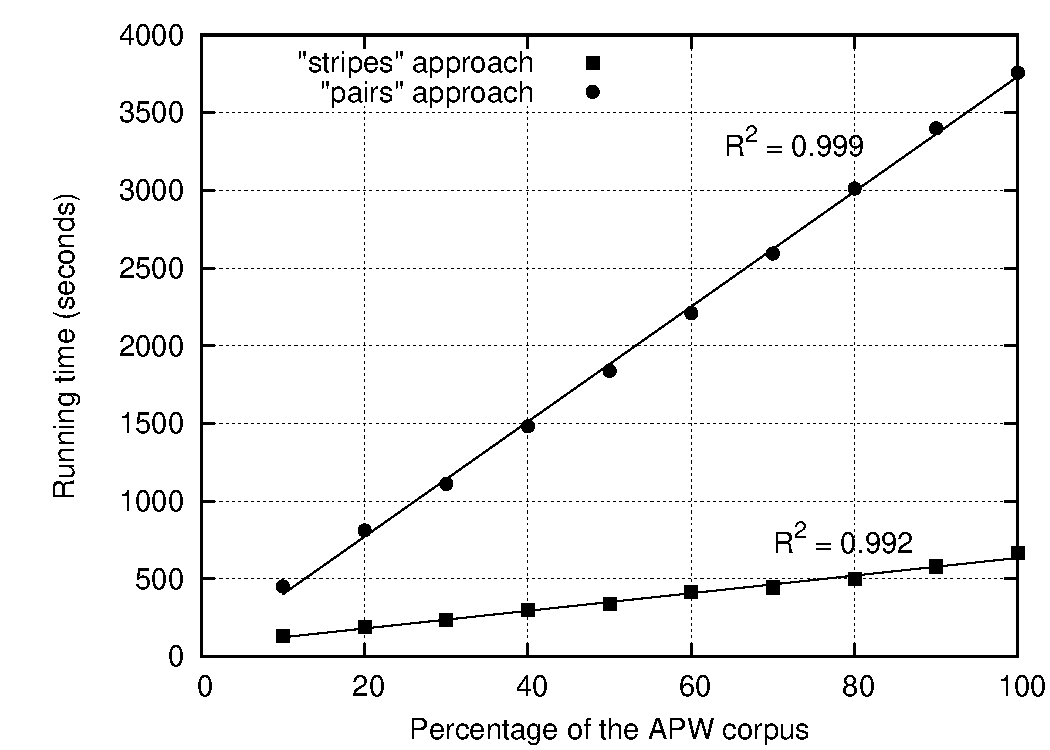
\includegraphics[scale=0.6]{figures/fig-ch3-pairs-vs-stripes.pdf}
\vspace{-0.3cm}
\end{center}
\caption{Running time of the ``pairs'' and ``stripes'' algorithms for
  computing word co-occurrence matrices on different fractions of the
  APW corpus.  These experiments were performed on a Hadoop cluster
  with 19 slaves, each with two single-core processors and two disks.}
\label{figure:chapter3:pairs-vs-stripes}
\end{figure}

\begin{figure}[p]
\begin{center}
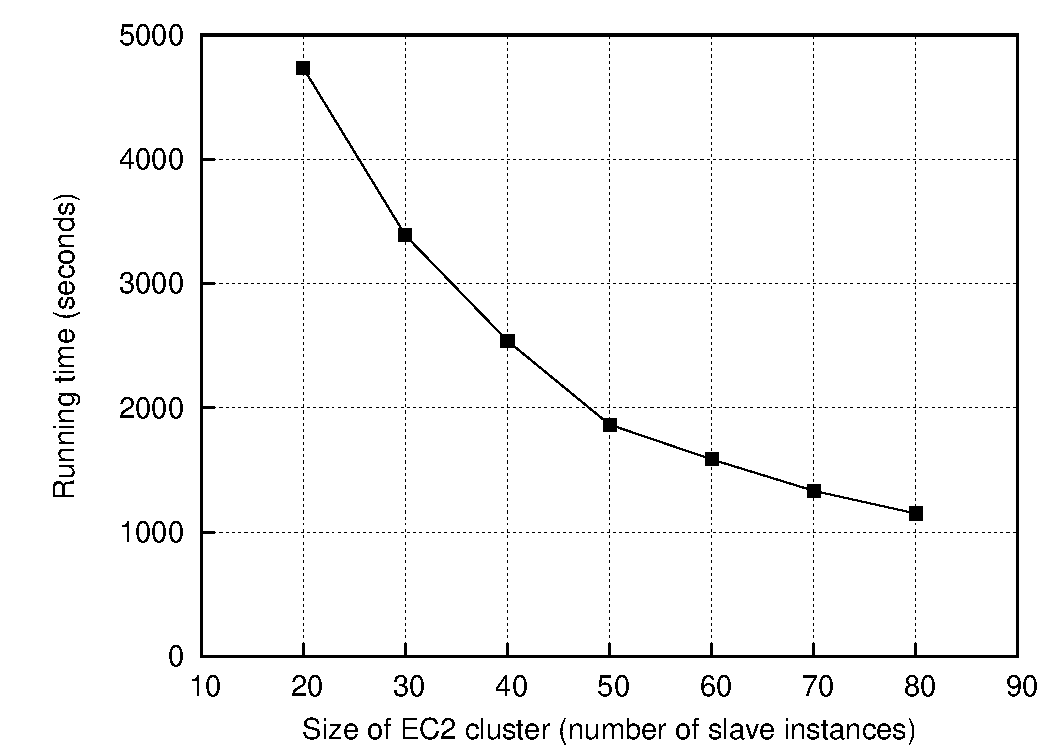
\includegraphics[scale=0.40]{figures/fig-ch3-pairs-vs-stripes-ec2a.pdf}
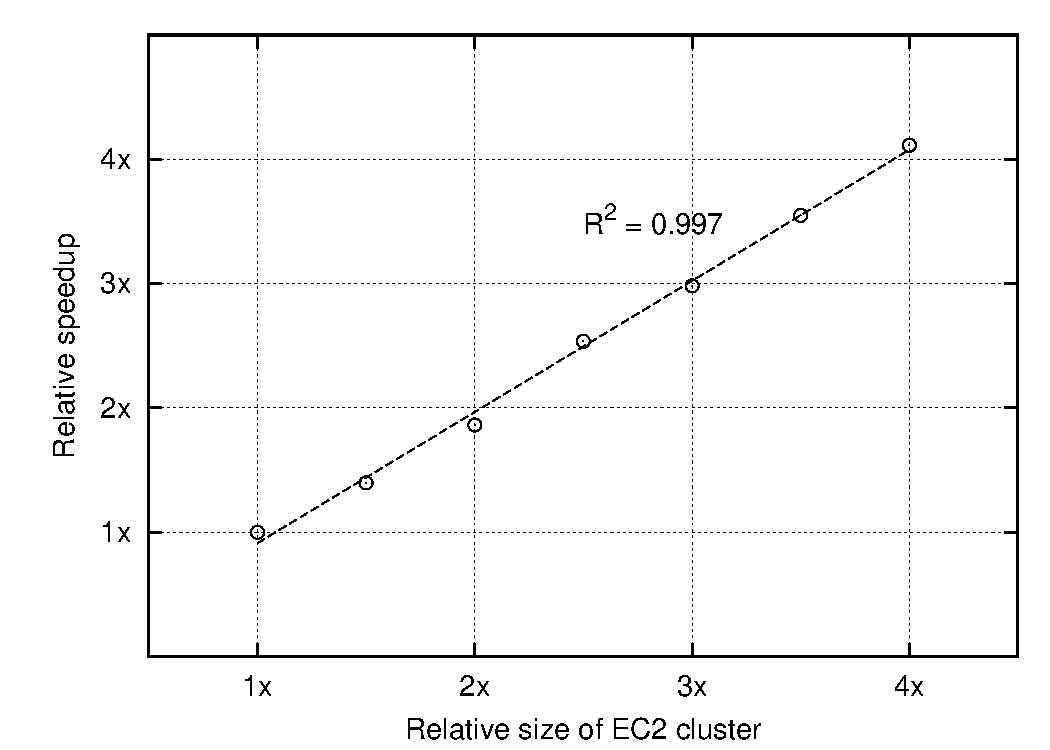
\includegraphics[scale=0.40]{figures/fig-ch3-pairs-vs-stripes-ec2b.pdf}
\vspace{-0.3cm}
\end{center}
\caption{Running time of the stripes algorithm on the APW corpus with
  Hadoop clusters of different sizes from EC2 (left).  Scaling
  characteristics (relative speedup) in terms of increasing Hadoop
  cluster size (right).}
\label{figure:chapter3:pairs-vs-stripes-ec2}
\end{figure}

An additional series of experiments explored the scalability of the
stripes approach along another dimension:\ the size of the cluster.
These experiments were made possible by Amazon's EC2 service, which
allows users to rapidly provision clusters of varying sizes for
limited durations (for more information, refer back to our discussion
of utility computing in Section~\ref{chapter1:clouds}).  Virtualized
computational units in EC2 are called instances, and the user is
charged only for the instance-hours consumed.
Figure~\ref{figure:chapter3:pairs-vs-stripes-ec2} (left) shows the
running time of the stripes algorithm (on the same corpus, with same
setup as before), on varying cluster sizes, from 20 slave ``small''
instances all the way up to 80 slave ``small'' instances (along the
{\it x}-axis).  Running times are shown with solid squares.
Figure~\ref{figure:chapter3:pairs-vs-stripes-ec2} (right) recasts the
same results to illustrate scaling characteristics.  The circles plot
the relative size and speedup of the EC2 experiments, with respect to
the 20-instance cluster.  These results show highly desirable linear
scaling characteristics (i.e., doubling the cluster size makes the job
twice as fast).  This is confirmed by a linear regression with an
$R^2$ value close to one.

Viewed abstractly, the pairs and stripes algorithms represent two
different approaches to counting co-occurring events from a large
number of observations.  This general description captures the gist of
many algorithms in fields as diverse as text processing, data mining,
and bioinformatics.  For this reason, these two design patterns are
broadly useful and frequently observed in a variety of applications.

To conclude, it is worth noting that the pairs and stripes approaches
represent endpoints along a continuum of possibilities.  The pairs
approach individually records {\it each} co-occurring event, while the
stripes approach records {\it all} co-occurring events with respect a
conditioning event.  A middle ground might be to record a subset of
the co-occurring events with respect to a conditioning event.  We
might divide up the entire vocabulary into $b$ buckets (e.g., via
hashing), so that words co-occurring with $w_i$ would be divided into
$b$ smaller ``sub-stripes'', associated with ten separate keys,
$(w_i,1), (w_i,2) \ldots (w_i,b)$.  This would be a reasonable
solution to the memory limitations of the stripes approach, since each
of the sub-stripes would be smaller.  In the case of $b=|V|$, where
$|V|$ is the vocabulary size, this is equivalent to the pairs
approach.  In the case of $b=1$, this is equivalent to the standard
stripes approach.

\section{Computing Relative Frequencies}
\label{chapter3:cond-prob}

Let us build on the pairs and stripes algorithms presented in the
previous section and continue with our running example of constructing
the word co-occurrence matrix $M$ for a large corpus.  Recall that in
this large square $n \times n$ matrix, where $n=|V|$ (the vocabulary
size), cell $m_{ij}$ contains the number of times word $w_i$ co-occurs
with word $w_j$ within a specific context.  The drawback of absolute
counts is that it doesn't take into account the fact that some words
appear more frequently than others.  Word $w_i$ may co-occur
frequently with $w_j$ simply because one of the words is very common.
A simple remedy is to convert absolute counts into relative
frequencies, $f(w_j|w_i)$.  That is, what proportion of the time does
$w_j$ appear in the context of $w_i$?  This can be computed using the
following equation:

\begin{equation}
f(w_j|w_i) = \frac{N(w_i,w_j)}{\sum_{w'}{N(w_i,w')}}
\end{equation}

\noindent Here, $N(\cdot, \cdot)$ indicates the number of times a
particular co-occurring word pair is observed in the corpus.  We need
the count of the joint event (word co-occurrence), divided by what is
known as the marginal (the sum of the counts of the conditioning
variable co-occurring with anything else).

Computing relative frequencies with the stripes approach is
straightforward.  In the reducer, counts of all words that co-occur
with the conditioning variable ($w_i$ in the above example) are
available in the associative array.  Therefore, it suffices to sum all
those counts to arrive at the marginal (i.e., $\sum_{w'}{N(w_i,w')}$),
and then divide all the joint counts by the marginal to arrive at the
relative frequency for all words.  This implementation requires
minimal modification to the original stripes algorithm in
Figure~\ref{figure:chapter3:coocur:stripes}, and illustrates the use
of complex data structures to coordinate distributed computations in
MapReduce.  Through appropriate structuring of keys and values, one
can use the MapReduce execution framework to bring together all the
pieces of data required to perform a computation.  Note that, as with
before, this algorithm also assumes that each associative array fits
into memory.

How might one compute relative frequencies with the pairs approach?
In the pairs approach, the reducer receives $(w_i, w_j)$ as the key and
the count as the value.  From this alone it is not possible to compute
$f(w_j|w_i)$ since we do not have the marginal.  Fortunately, as in the
mapper, the reducer can preserve state across multiple keys.  Inside
the reducer, we can buffer in memory all the words that co-occur with
$w_i$ and their counts, in essence building the associative array in the
stripes approach.  To make this work, we must define the sort order of
the pair so that keys are first sorted by the left word, and then by
the right word.  Given this ordering, we can easily detect if all
pairs associated with the word we are conditioning on ($w_i$) have been
encountered.  At that point we can go back through the in-memory
buffer, compute the relative frequencies, and then emit those results
in the final key-value pairs.

There is one more modification necessary to make this algorithm work.
We must ensure that all pairs with the same left word are sent to the
same reducer.  This, unfortunately, does not happen
automatically:\ recall that the default partitioner is based on the
hash value of the intermediate key, modulo the number of reducers.
For a complex key, the raw byte representation is used to compute the
hash value.  As a result, there is no guarantee that, for example,
(dog, aardvark) and (dog, zebra) are assigned to the same reducer.  To
produce the desired behavior, we must define a custom partitioner that
only pays attention to the left word.  That is, the partitioner should
partition based on the hash of the left word only.

This algorithm will indeed work, but it suffers from the same drawback
as the stripes approach:\ as the size of the corpus grows, so does
that vocabulary size, and at some point there will not be sufficient
memory to store all co-occurring words and their counts for the word
we are conditioning on.  For computing the co-occurrence matrix, the
advantage of the pairs approach is that it doesn't suffer from any
memory bottlenecks.  Is there a way to modify the basic pairs approach
so that this advantage is retained?

As it turns out, such an algorithm is indeed possible, although it
requires the coordination of several mechanisms in MapReduce.  The
insight lies in properly sequencing data presented to the reducer.  If
it were possible to somehow compute (or otherwise obtain access to)
the marginal in the reducer before processing the joint counts, the
reducer could simply divide the joint counts by the marginal to
compute the relative frequencies.  The notion of ``before'' and
``after'' can be captured in the ordering of key-value pairs, which
can be explicitly controlled by the programmer.  That is, the
programmer can define the sort order of keys so that data needed
earlier is presented to the reducer before data that is needed later.
However, we still need to compute the marginal counts.  Recall that in
the basic pairs algorithm, each mapper emits a key-value pair with the
co-occurring word pair as the key.  To compute relative frequencies,
we modify the mapper so that it additionally emits a ``special'' key
of the form $(w_i, \ast)$, with a value of one, that represents the
contribution of the word pair to the marginal.  Through use of
combiners, these partial marginal counts will be aggregated before
being sent to the reducers.  Alternatively, the in-mapper combining
pattern can be used to even more efficiently aggregate marginal
counts.

In the reducer, we must make sure that the special key-value pairs
representing the partial marginal contributions are processed before
the normal key-value pairs representing the joint counts.  This is
accomplished by defining the sort order of the keys so that pairs with
the special symbol of the form $(w_i, \ast)$ are ordered before any other
key-value pairs where the left word is $w_i$.  In addition, as with
before we must also properly define the partitioner to pay attention
to only the left word in each pair.  With the data properly sequenced,
the reducer can directly compute the relative frequencies.

\begin{figure}[t]
\begin{tabular}{lll}
{\bf key} & {\bf values} &  \\
$(\textrm{dog}, \ast)$        & $[$6327, 8514, $\ldots$$]$ & compute marginal: $\sum_{w'}{N(\textrm{dog},w')} = 42908$\\
$(\textrm{dog}, \textrm{aardvark})$ & $[$2,1$]$    & $f(\textrm{aardvark}|\textrm{dog}) = 3/42908$ \\
$(\textrm{dog}, \textrm{aardwolf})$ & $[$1$]$      & $f(\textrm{aardwolf}|\textrm{dog}) = 1/42908$ \\
\ldots            &      & \\
$(\textrm{dog}, \textrm{zebra})$    & $[$2,1,1,1$]$    & $f(\textrm{zebra}|\textrm{dog}) = 5/42908$ \\
$(\textrm{doge}, \ast)$       & $[$682, $\ldots$$]$  & compute marginal: $\sum_{w'}{N(\textrm{doge},w')} = 1267$\\
\ldots            &      & \\
\end{tabular}
\caption{Example of the sequence of key-value pairs presented to the
  reducer in the pairs algorithm for computing relative frequencies.
  This illustrates the application of the order inversion design
  pattern.}
\label{figure:chapter3:cond-prob-reducer}
\end{figure}

A concrete example is shown in
Figure~\ref{figure:chapter3:cond-prob-reducer}, which lists the
sequence of key-value pairs that a reducer might encounter.  First,
the reducer is presented with the special key $(\textrm{dog}, \ast)$
and a number of values, each of which represents a partial marginal
contribution from the map phase (assume here either combiners or
in-mapper combining, so the values represent partially aggregated
counts).  The reducer accumulates these counts to arrive at the
marginal, $\sum_{w'}{N(\textrm{dog},w')}$.  The reducer holds on to
this value as it processes subsequent keys.  After $(\textrm{dog},
\ast)$, the reducer will encounter a series of keys representing joint
counts; let's say the first of these is the key $(\textrm{dog},
\textrm{aardvark})$.  Associated with this key will be a list of
values representing partial joint counts from the map phase (two
separate values in this case).  Summing these counts will yield the
final joint count, i.e., the number of times dog and aardvark co-occur
in the entire collection.  At this point, since the reducer already
knows the marginal, simple arithmetic suffices to compute the relative
frequency.  All subsequent joint counts are processed in exactly the
same manner.  When the reducer encounters the next special key-value
pair $(\textrm{doge}, \ast)$, the reducer resets its internal state
and starts to accumulate the marginal all over again.  Observe that
the memory requirement for this algorithm is minimal, since only the
marginal (an integer) needs to be stored.  No buffering of individual
co-occurring word counts is necessary, and therefore we have
eliminated the scalability bottleneck of the previous algorithm.

This design pattern, which we call ``order inversion'', occurs
surprisingly often and across applications in many domains.  It is so
named because through proper coordination, we can access the result of
a computation in the reducer (for example, an aggregate statistic)
before processing the data needed for that computation.  The key
insight is to convert the sequencing of computations into a sorting
problem.  In most cases, an algorithm requires data in some fixed
order:\ by controlling how keys are sorted and how the key space is
partitioned, we can present data to the reducer in the order necessary
to perform the proper computations.  This greatly cuts down on the
amount of partial results that the reducer needs to hold in memory.

To summarize, the specific application of the order inversion design
pattern for computing relative frequencies requires the
following:

\begin{itemize}

\item Emitting a special key-value pair for each co-occurring word
  pair in the mapper to capture its contribution to the marginal.

\item Controlling the sort order of the intermediate key so that the
  key-value pairs representing the marginal contributions are
  processed by the reducer before any of the pairs representing the
  joint word co-occurrence counts.

\item Defining a custom partitioner to ensure that all pairs with the
  same left word are shuffled to the same reducer.

\item Preserving state across multiple keys in the reducer to first
  compute the marginal based on the special key-value pairs and then
  dividing the joint counts by the marginals to arrive at the
  relative frequencies.

\end{itemize}

\noindent As we will see in Chapter~\ref{chapter-indexing}, this design
pattern is also used in inverted index construction to properly set
compression parameters for postings lists.

\section{Secondary Sorting}
\label{chapter3:secondary-sorting}

MapReduce sorts intermediate key-value pairs by the keys during the
shuffle and sort phase, which is very convenient if computations
inside the reducer rely on sort order (e.g., the order inversion
design pattern described in the previous section).  However, what if
in addition to sorting by key, we also need to sort by value?
Google's MapReduce implementation provides built-in functionality for
(optional) secondary sorting, which guarantees that values arrive in
sorted order.  Hadoop, unfortunately, does not have this capability
built in.

Consider the example of sensor data from a scientific
experiment:\ there are $m$ sensors each taking readings on continuous
basis, where $m$ is potentially a large number.  A dump of the sensor
data might look something like the following, where $r_x$ after
each timestamp represents the actual sensor readings (unimportant for
this discussion, but may be a series of values, one or more complex
records, or even raw bytes of images).

\begin{quote}
$(t_1, m_1, r_{80521})$\\
$(t_1, m_2, r_{14209})$\\
$(t_1, m_3, r_{76042})$\\
$...$\\
$(t_2, m_1, r_{21823})$\\
$(t_2, m_2, r_{66508})$\\
$(t_2, m_3, r_{98347})$
\end{quote}

\noindent Suppose we wish to reconstruct the activity at each
individual sensor over time.  A MapReduce program to accomplish this
might map over the raw data and emit the sensor id as the intermediate
key, with the rest of each record as the value:

\begin{quote}
$m_1 \rightarrow (t_1, r_{80521})$
\end{quote}

\noindent This would bring all readings from the same sensor together
in the reducer.  However, since MapReduce makes no guarantees about
the ordering of values associated with the same key, the sensor
readings will not likely be in temporal order.  The most obvious
solution is to buffer all the readings in memory and then sort by
timestamp before additional processing.  However, it should be
apparent by now that any in-memory buffering of data introduces a
potential scalability bottleneck.  What if we are working with a high
frequency sensor or sensor readings over a long period of time?  What
if the sensor readings themselves are large complex objects?  This
approach may not scale in these cases---the reducer would run out of
memory trying to buffer all values associated with the same key.

This is a common problem, since in many applications we wish to first
group together data one way (e.g., by sensor id), and then sort within
the groupings another way (e.g., by time).  Fortunately, there is a
general purpose solution, which we call the ``value-to-key
conversion'' design pattern.  The basic idea is to move part of the
value into the intermediate key to form a composite key, and let the
MapReduce execution framework handle the sorting.  In the above
example, instead of emitting the sensor id as the key, we would emit
the sensor id and the timestamp as a composite key:

\begin{quote}
$(m_1, t_1) \rightarrow (r_{80521})$
\end{quote}

\noindent The sensor reading itself now occupies the value.  We must
define the intermediate key sort order to first sort by the sensor id
(the left element in the pair) and then by the timestamp (the right
element in the pair).  We must also implement a custom partitioner so
that all pairs associated with the same sensor are shuffled to the
same reducer.

Properly orchestrated, the key-value pairs will be presented to the
reducer in the correct sorted order:

\begin{quote}
$(m_1, t_1) \rightarrow [(r_{80521})]$ \\
$(m_1, t_2) \rightarrow [(r_{21823})]$ \\
$(m_1, t_3) \rightarrow [(r_{146925})]$ \\
$\ldots$
\end{quote}

\noindent However, note that sensor readings are now split across
multiple keys.  The reducer will need to preserve state and keep track
of when readings associated with the current sensor end and the next
sensor begin.\footnote{Alternatively, Hadoop provides API hooks to
  define ``groups'' of intermediate keys that should be processed
  together in the reducer.}

The basic tradeoff between the two approaches discussed above (buffer
and in-memory sort vs.\ value-to-key conversion) is where sorting is
performed.  One can explicitly implement secondary sorting in the
reducer, which is likely to be faster but suffers from a scalability
bottleneck.\footnote{Note that, in principle, this need not be an
  in-memory sort.  It is entirely possible to implement a disk-based
  sort within the reducer, although one would be duplicating
  functionality that is already present in the MapReduce execution
  framework.  It makes more sense to take advantage of functionality
  that is already present with value-to-key conversion.}  With
value-to-key conversion, sorting is offloaded to the MapReduce
execution framework.  Note that this approach can be arbitrarily
extended to tertiary, quaternary, etc.\ sorting.  This pattern results
in many more keys for the framework to sort, but distributed sorting
is a task that the MapReduce runtime excels at since it lies at the
heart of the programming model.

\section{Relational Joins}
\label{chapter3:joins}

One popular application of Hadoop is data-warehousing.  In an
enterprise setting, a data warehouse serves as a vast repository of
data, holding everything from sales transactions to product
inventories.  Typically, the data is relational in nature, but
increasingly data warehouses are used to store semi-structured data
(e.g., query logs) as well as unstructured data.  Data warehouses form
a foundation for business intelligence applications designed to
provide decision support.  It is widely believed that insights gained
by mining historical, current, and prospective data can yield
competitive advantages in the marketplace.

Traditionally, data warehouses have been implemented through
relational databases, particularly those optimized for a specific
workload known as online analytical processing (OLAP).  A number of
vendors offer parallel databases, but customers find that they often
cannot cost-effectively scale to the crushing amounts of data an
organization needs to deal with today.  Parallel databases are often
quite expensive---on the order of tens of thousands of dollars per
terabyte of user data.  Over the past few years, Hadoop has gained
popularity as a platform for data-warehousing.
Hammerbacher~\cite{Hammerbacher_2009}, for example, discussed
Facebook's experiences with scaling up business intelligence
applications with Oracle databases, which they ultimately abandoned in
favor of a Hadoop-based solution developed in-house called Hive (which
is now an open-source project).  Pig~\cite{Olston_etal_SIGMOD2008} is
a platform for massive data analytics built on Hadoop and capable of
handling structured as well as semi-structured data.  It was
originally developed by Yahoo, but is now also an open-source project.

Given successful applications of Hadoop to data-warehousing and
complex analytical queries that are prevalent in such an environment,
it makes sense to examine MapReduce algorithms for manipulating
relational data.  This section focuses specifically on performing
relational joins in MapReduce.  We should stress here that even though
Hadoop has been applied to process relational data, Hadoop {\it is not
  a database}.  There is an ongoing debate between advocates of
parallel databases and proponents of MapReduce regarding the merits of
both approaches for OLAP-type workloads.  Dewitt and Stonebraker, two
well-known figures in the database community, famously decried
MapReduce as ``a major step backwards'' in a controversial blog
post.\footnote{\tt
  http://databasecolumn.vertica.com/database-innovation/mapreduce-a-major-step-backwards/}
With colleagues, they ran a series of benchmarks that demonstrated the
supposed superiority of column-oriented parallel databases over
Hadoop~\cite{Pavlo_etal_SIGMOD2009,Stonebraker_etal_CACM2010}. However,
see Dean and Ghemawat's counterarguments~\cite{Dean_Ghemawat_CACM2010}
and recent attempts at hybrid
architectures~\cite{Abouzeid_etal_VLDB2009}.

We shall refrain here from participating in this lively debate, and
instead focus on discussing algorithms.  From an application point of
view, it is highly unlikely that an analyst interacting with a data
warehouse will ever be called upon to write MapReduce programs (and
indeed, Hadoop-based systems such as Hive and Pig present a much
higher-level language for interacting with large amounts of data).
Nevertheless, it is instructive to understand the algorithms that
underlie basic relational operations.

This section presents three different strategies for performing
relational joins on two datasets (relations), generically named $S$
and $T$.  Let us suppose that relation $S$ looks something like the
following:

\begin{quote}
$(k_1, s_1, \textbf{S}_1)$ \\
$(k_2, s_2, \textbf{S}_2)$ \\
$(k_3, s_3, \textbf{S}_3)$ \\
$\ldots$
\end{quote}

\noindent where $k$ is the key we would like to join on, $s_n$ is a
unique id for the tuple, and the $\textbf{S}_n$ after $s_n$ denotes
other attributes in the tuple (unimportant for the purposes of the
join).  Similarly, suppose relation $T$ looks something like this:

\begin{quote}
$(k_1, t_1, \textbf{T}_1)$ \\
$(k_3, t_2, \textbf{T}_2)$ \\
$(k_8, t_3, \textbf{T}_3)$ \\
$\ldots$
\end{quote}

\noindent where $k$ is the join key, $t_n$ is a unique id for the
tuple, and the $\textbf{T}_n$ after $t_n$ denotes other attributes in the
tuple.  

To make this task more concrete, we present one realistic
scenario:\ $S$ might represent a collection of user profiles, in which
case $k$ could be interpreted as the primary key (i.e., user id).  The
tuples might contain demographic information such as age, gender,
income, etc.  The other dataset, $T$, might represent logs of online
activity.  Each tuple might correspond to a page view of a particular
URL and may contain additional information such as time spent on the
page, ad revenue generated, etc.  The $k$ in these tuples could be
interpreted as the foreign key that associates each individual page
view with a user.  Joining these two datasets would allow an analyst,
for example, to break down online activity in terms of demographics.

\subsection{Reduce-Side Join}

The first approach to relational joins is what's known as a {\it
  reduce-side} join.  The idea is quite simple:\ we map over both
datasets and emit the join key as the intermediate key, and the tuple
itself as the intermediate value.  Since MapReduce guarantees that all
values with the same key are brought together, all tuples will be
grouped by the join key---which is exactly what we need to perform the
join operation.  This approach is known as a parallel sort-merge join
in the database community~\cite{Schneider_DeWitt_SIGMOD1989}.  In more
detail, there are three different cases to consider.

The first and simplest is a {\it one-to-one} join, where at most one
tuple from $S$ and one tuple from $T$ share the same join key (but
it may be the case that no tuple from $S$ shares the join key with a
tuple from $T$, or vice versa).  In this case, the algorithm sketched
above will work fine.  The reducer will be presented keys and lists of
values along the lines of the following:

\begin{quote}
$k_{23} \rightarrow [ (s_{64}, \textbf{S}_{64}), (t_{84}, \textbf{T}_{84}) ]$ \\
$k_{37} \rightarrow [ (s_{68}, \textbf{S}_{68}) ]$ \\
$k_{59} \rightarrow [ (t_{97}, \textbf{T}_{97}), (s_{81}, \textbf{S}_{81}) ]$ \\
$k_{61} \rightarrow [ (t_{99}, \textbf{T}_{99}) ]$ \\
$\ldots$
\end{quote}

\noindent Since we've emitted the join key as the intermediate key, we
can remove it from the value to save a bit of space.\footnote{Not very
  important if the intermediate data is compressed.}  If there are two
values associated with a key, then we know that one must be from $S$
and the other must be from $T$.  However, recall that in the basic
MapReduce programming model, no guarantees are made about value
ordering, so the first value might be from $S$ or from $T$.  We can
proceed to join the two tuples and perform additional computations
(e.g., filter by some other attribute, compute aggregates, etc.).  If
there is only one value associated with a key, this means that no
tuple in the other dataset shares the join key, so the reducer does
nothing.

Let us now consider the {\it one-to-many} join.  Assume that tuples in
$S$ have unique join keys (i.e., $k$ is the primary key in $S$), so
that $S$ is the ``one'' and $T$ is the ``many''.  The above algorithm
will still work, but when processing each key in the reducer, we have
no idea when the value corresponding to the tuple from $S$ will be
encountered, since values are arbitrarily ordered.  The easiest
solution is to buffer all values in memory, pick out the tuple from
$S$, and then cross it with every tuple from $T$ to perform the join.
However, as we have seen several times already, this creates a
scalability bottleneck since we may not have sufficient memory to hold
all the tuples with the same join key.

This is a problem that requires a secondary sort, and the solution
lies in the value-to-key conversion design pattern we just presented.
In the mapper, instead of simply emitting the join key as the
intermediate key, we instead create a composite key consisting of the
join key and the tuple id (from either $S$ or $T$).  Two additional
changes are required: First, we must define the sort order of the keys
to first sort by the join key, and then sort all tuple ids from $S$
before all tuple ids from $T$.  Second, we must define the
partitioner to pay attention to only the join key, so that all
composite keys with the same join key arrive at the same reducer.

After applying the value-to-key conversion design pattern, the reducer
will be presented with keys and values along the lines of the
following:

\begin{quote}
$(k_{82}, s_{105}) \rightarrow [(\textbf{S}_{105})]$ \\
$(k_{82}, t_{98}) \rightarrow [(\textbf{T}_{98})]$ \\
$(k_{82}, t_{101}) \rightarrow [(\textbf{T}_{101})]$ \\
$(k_{82}, t_{137}) \rightarrow [(\textbf{T}_{137})]$ \\
$\ldots$
\end{quote}

\noindent Since both the join key and the tuple id are present in the
intermediate key, we can remove them from the value to save a bit of
space.\footnote{Once again, not very important if the intermediate
  data is compressed.}  Whenever the reducer encounters a new join
key, it is guaranteed that the associated value will be the relevant
tuple from $S$.  The reducer can hold this tuple in memory and then
proceed to cross it with tuples from $T$ in subsequent steps (until a
new join key is encountered).  Since the MapReduce execution framework
performs the sorting, there is no need to buffer tuples (other than
the single one from $S$).  Thus, we have eliminated the scalability
bottleneck.

Finally, let us consider the {\it many-to-many} join case.  Assuming
that $S$ is the smaller dataset, the above algorithm works as well.
Consider what happens at the reducer:

\begin{quote}
$(k_{82}, s_{105}) \rightarrow [(\textbf{S}_{105})]$ \\
$(k_{82}, s_{124}) \rightarrow [(\textbf{S}_{124})]$ \\
$\ldots$ \\
$(k_{82}, t_{98})  \rightarrow [(\textbf{T}_{98})]$ \\
$(k_{82}, t_{101}) \rightarrow [(\textbf{T}_{101})]$ \\
$(k_{82}, t_{137}) \rightarrow [(\textbf{T}_{137})]$ \\
$\ldots$
\end{quote}

\noindent All the tuples from $S$ with the same join key will be
encountered first, which the reducer can buffer in memory.  As the
reducer processes each tuple from $T$, it is crossed with all the
tuples from $S$.  Of course, we are assuming that the tuples from $S$
(with the same join key) will fit into memory, which is a limitation
of this algorithm (and why we want to control the sort order so that
the smaller dataset comes first).

The basic idea behind the reduce-side join is to repartition the two
datasets by the join key.  The approach isn't particularly efficient
since it requires shuffling both datasets across the network.  This
leads us to the {\it map-side} join.

\subsection{Map-Side Join}

Suppose we have two datasets that are both sorted by the join key.  We
can perform a join by scanning through both datasets
simultaneously---this is known as a merge join in the database
community.  We can parallelize this by partitioning and sorting {\it
  both} datasets in the same way.  For example, suppose $S$ and $T$
were both divided into ten files, partitioned in the same manner by
the join key.  Further suppose that in each file, the tuples were
sorted by the join key.  In this case, we simply need to merge join
the first file of $S$ with the first file of $T$, the second file with
$S$ with the second file of $T$, etc.  This can be accomplished in
parallel, in the map phase of a MapReduce job---hence, a {\it
  map-side} join.  In practice, we map over one of the datasets (the
larger one) and inside the mapper read the corresponding part of the
other dataset to perform the merge join.\footnote{Note that this
  almost always implies a non-local read.}  No reducer is required,
unless the programmer wishes to repartition the output or perform
further processing.

A map-side join is far more efficient than a reduce-side join since
there is no need to shuffle the datasets over the network.  But is it
realistic to expect that the stringent conditions required for
map-side joins are satisfied?  In many cases, {\it yes}.  The reason
is that relational joins happen within the broader context of a
workflow, which may include multiple steps.  Therefore, the datasets
that are to be joined may be the output of previous processes (either
MapReduce jobs or other code).  If the workflow is known in advance
and relatively static (both reasonable assumptions in a mature
workflow), we can engineer the previous processes to generate
output sorted and partitioned in a way that makes efficient map-side
joins possible (in MapReduce, by using a custom partitioner and
controlling the sort order of key-value pairs).  For {\it ad hoc} data
analysis, reduce-side joins are a more general, albeit less efficient,
solution.  Consider the case where datasets have multiple keys that
one might wish to join on---then no matter how the data is organized,
map-side joins will require repartitioning of the data.
Alternatively, it is always possible to repartition a dataset using an
identity mapper and reducer.  But of course, this incurs the cost of
shuffling data over the network.

There is a final restriction to bear in mind when using map-side joins
with the Hadoop implementation of MapReduce.  We assume here that the
datasets to be joined were produced by previous MapReduce jobs, so
this restriction applies to keys the reducers in those jobs may emit.
Hadoop permits reducers to emit keys that are different from the
input key whose values they are processing (that is, input and output
keys need not be the same, nor even the same type).\footnote{In
  contrast, recall from Section~\ref{chapter2:mappers-and-reducers}
  that in Google's implementation, reducers' output keys must be
  exactly same as their input keys.}  However, if the output key of a
reducer is different from the input key, then the output dataset from
the reducer will not necessarily be partitioned in a manner consistent
with the specified partitioner (because the partitioner applies to the
\emph{input} keys rather than the \emph{output} keys).  Since map-side
joins depend on consistent partitioning and sorting of keys, the
reducers used to generate data that will participate in a later
map-side join \emph{must not} emit any key but the one they are
currently processing.

\subsection{Memory-Backed Join}

In addition to the two previous approaches to joining relational data
that leverage the MapReduce framework to bring together tuples that
share a common join key, there is a family of approaches we call
\emph{memory-backed} joins based on random access probes.  The
simplest version is applicable when one of the two datasets completely
fits in memory on each node.  In this situation, we can load the
smaller dataset into memory in every mapper, populating an associative
array to facilitate random access to tuples based on the join key.
The mapper initialization API hook (see
Section~\ref{chapter3:local-aggregation:combiners}) can be used for
this purpose.  Mappers are then applied to the other (larger) dataset,
and for each input key-value pair, the mapper probes the in-memory
dataset to see if there is a tuple with the same join key.  If there
is, the join is performed.  This is known as a simple hash join by the
database community~\cite{DeWitt_etal_1984}.

What if neither dataset fits in memory?  The simplest solution is to
divide the smaller dataset, let's say $S$, into $n$ partitions, such
that $S= S_1 \cup S_2 \cup \ldots \cup S_n$.  We can choose $n$ so
that each partition is small enough to fit in memory, and then run $n$
memory-backed hash joins.  This, of course, requires streaming through
the other dataset $n$ times.

There is an alternative approach to memory-backed joins for cases
where neither datasets fit into memory.  A distributed key-value store
can be used to hold one dataset in memory across multiple machines
while mapping over the other.  The mappers would then query this
distributed key-value store in parallel and perform joins if the join
keys match.\footnote{In order to achieve good performance in accessing
  distributed key-value stores, it is often necessary to batch queries
  before making synchronous requests (to amortize latency over many
  requests) or to rely on asynchronous requests.}  The open-source
caching system memcached can be used for exactly this purpose, and
therefore we've dubbed this approach {\it memcached} join.  For more
information, this approach is detailed in a technical
report~\cite{Lin_etal_TR2009}.

\section{Summary}

This chapter provides a guide on the design of MapReduce algorithms.
In particular, we present a number of ``design patterns'' that capture
effective solutions to common problems.  In summary, they are:

\begin{itemize}

\item ``In-mapper combining'', where the functionality of the combiner
  is moved into the mapper.  Instead of emitting intermediate output
  for every input key-value pair, the mapper aggregates partial
  results across multiple input records and only emits intermediate
  key-value pairs after some amount of local aggregation is performed.

\item The related patterns ``pairs'' and ``stripes'' for keeping track
  of joint events from a large number of observations.  In the pairs
  approach, we keep track of each joint event separately, whereas in
  the stripes approach we keep track of all events that co-occur with
  the same event.  Although the stripes approach is significantly more
  efficient, it requires memory on the order of the size of the event
  space, which presents a scalability bottleneck.

\item ``Order inversion'', where the main idea is to convert the
  sequencing of computations into a sorting problem.  Through careful
  orchestration, we can send the reducer the result of a computation
  (e.g., an aggregate statistic) before it encounters the data
  necessary to produce that computation.

\item ``Value-to-key conversion'', which provides a scalable solution
  for secondary sorting.  By moving part of the value into the key, we
  can exploit the MapReduce execution framework itself for sorting.

\end{itemize}

\noindent Ultimately, controlling synchronization in the MapReduce
programming model boils down to effective use of the following
techniques:

\begin{enumerate}

\item Constructing complex keys and values that bring together data
  necessary for a computation.  This is used in all of the above
  design patterns.

\item Executing user-specified initialization and termination code in
  either the mapper or reducer.  For example, in-mapper combining
  depends on emission of intermediate key-value pairs in the map task
  termination code.

\item Preserving state across multiple inputs in the mapper and
  reducer.  This is used in in-mapper combining, order inversion, and
  value-to-key conversion.

\item Controlling the sort order of intermediate keys.  This is used
  in order inversion and value-to-key conversion.

\item Controlling the partitioning of the intermediate key space.
  This is used in order inversion and value-to-key conversion.

\end{enumerate}

\noindent This concludes our overview of MapReduce algorithm design.
It should be clear by now that although the programming model forces
one to express algorithms in terms of a small set of rigidly-defined
components, there are many tools at one's disposal to shape the flow
of computation.  In the next few chapters, we will focus on specific
classes of MapReduce algorithms:\ for inverted indexing in
Chapter~\ref{chapter-indexing}, for graph processing in
Chapter~\ref{chapter-graphs}, and for expectation-maximization in
Chapter~\ref{chapter6}.

\chapter{Inverted Indexing for Text Retrieval}
\label{chapter-indexing}

Web search is the quintessential large-data problem.  Given an
information need expressed as a short query consisting of a few terms,
the system's task is to retrieve relevant web objects (web pages, PDF
documents, PowerPoint slides, etc.) and present them to the user.  How
large is the web?  It is difficult to compute exactly, but even a
conservative estimate would place the size at several tens of billions
of pages, totaling hundreds of terabytes (considering text alone).  In
real-world applications, users demand results quickly from a search
engine---query latencies longer than a few hundred milliseconds will
try a user's patience.  Fulfilling these requirements is quite an
engineering feat, considering the amounts of data involved!

Nearly all retrieval engines for full-text search today rely on a data
structure called an inverted index, which given a term provides access
to the list of documents that contain the term.  In information
retrieval parlance, objects to be retrieved are generically called
``documents'' even though in actuality they may be web pages, PDFs, or
even fragments of code.  Given a user query, the retrieval engine uses
the inverted index to score documents that contain the query terms
with respect to some ranking model, taking into account features such
as term matches, term proximity, attributes of the terms in the
document (e.g., bold, appears in title, etc.), as well as the
hyperlink structure of the documents (e.g.,
PageRank~\cite{Page_etal_1999}, which we'll discuss in
Chapter~\ref{chapter-graphs}, or related metrics such as
HITS~\cite{Kleinberg_JACM1999} and
SALSA~\cite{Lempel_Moran_TOIS2001}).  

The web search problem decomposes into three components:\ gathering
web content (crawling), construction of the inverted index (indexing)
and ranking documents given a query (retrieval).  Crawling and
indexing share similar characteristics and requirements, but these are
very different from retrieval.  Gathering web content and building
inverted indexes are for the most part offline problems.  Both need to
be scalable and efficient, but they do not need to operate in real
time.  Indexing is usually a batch process that runs
periodically:\ the frequency of refreshes and updates is usually
dependent on the design of the crawler.  Some sites (e.g., news
organizations) update their content quite frequently and need to be
visited often; other sites (e.g., government regulations) are
relatively static.  However, even for rapidly changing sites, it is
usually tolerable to have a delay of a few minutes until content is
searchable.  Furthermore, since the amount of content that changes
rapidly is relatively small, running smaller-scale index updates at
greater frequencies is usually an adequate solution.\footnote{Leaving
  aside the problem of searching live data streams such a tweets,
  which requires different techniques and algorithms.} Retrieval, on
the other hand, is an online problem that demands sub-second response
time.  Individual users expect low query latencies, but query
throughput is equally important since a retrieval engine must usually
serve many users concurrently.  Furthermore, query loads are highly
variable, depending on the time of day, and can exhibit ``spikey''
behavior due to special circumstances (e.g., a breaking news event
triggers a large number of searches on the same topic).  On the other
hand, resource consumption for the indexing problem is more
predictable.

A comprehensive treatment of web search is beyond the scope of this
chapter, and even this entire book.  Explicitly recognizing this, we
mostly focus on the problem of inverted indexing, the task most
amenable to solutions in MapReduce.  This chapter begins by first
providing an overview of web crawling
(Section~\ref{chapter-indexing:crawling}) and introducing the basic
structure of an inverted index (Section~\ref{chapter-indexing:intro}).
A baseline inverted indexing algorithm in MapReduce is presented in
Section~\ref{chapter-indexing:index:baseline}.  We point out a
scalability bottleneck in that algorithm, which leads to a revised
version presented in Section~\ref{chapter-indexing:index:revised}.
Index compression is discussed in
Section~\ref{chapter-indexing:index:compression}, which fills in
missing details on building compact index structures.  Since MapReduce
is primarily designed for batch-oriented processing, it does not
provide an adequate solution for the retrieval problem, an issue we
discuss in Section~\ref{chapter-indexing:retrieval}.  The chapter
concludes with a summary and pointers to additional readings.

\section{Web Crawling}
\label{chapter-indexing:crawling}

Before building inverted indexes, we must first acquire the document
collection over which these indexes are to be built.  In academia and
for research purposes, this can be relatively straightforward.
Standard collections for information retrieval research are widely
available for a variety of genres ranging from blogs to newswire text.
For researchers who wish to explore web-scale retrieval, there is the
ClueWeb09 collection that contains one billion web pages in ten
languages (totaling 25 terabytes) crawled by Carnegie Mellon
University in early 2009.\footnote{\texttt{
    http://boston.lti.cs.cmu.edu/Data/clueweb09/}} Obtaining access to
these standard collections is usually as simple as signing an
appropriate data license from the distributor of the collection,
paying a reasonable fee, and arranging for receipt of the
data.\footnote{As an interesting side note, in the 1990s, research
  collections were distributed via postal mail on CD-ROMs, and later,
  on DVDs.  Electronic distribution became common earlier this decade
  for collections below a certain size.  However, many collections
  today are so large that the only practical method of distribution is
  shipping hard drives via postal mail.}

For real-world web search, however, one cannot simply assume that the
collection is already available.  Acquiring web content requires
crawling, which is the process of traversing the web by repeatedly
following hyperlinks and storing downloaded pages for subsequent
processing.  Conceptually, the process is quite simple to
understand:\ we start by populating a queue with a ``seed'' list of
pages.  The crawler downloads pages in the queue, extracts links from
those pages to add to the queue, stores the pages for further
processing, and repeats.  In fact, rudimentary web crawlers can be
written in a few hundred lines of code.

However, effective and efficient web crawling is far more complex.
The following lists a number of issues that real-world crawlers must
contend with:

\begin{itemize}

\item A web crawler must practice good ``etiquette'' and not overload
  web servers.  For example, it is common practice to wait a fixed
  amount of time before repeated requests to the same server.  In
  order to respect these constraints while maintaining good
  throughput, a crawler typically keeps many execution threads running
  in parallel and maintains many TCP connections (perhaps hundreds)
  open at the same time.

\item Since a crawler has finite bandwidth and resources, it must
  prioritize the order in which unvisited pages are downloaded.  Such
  decisions must be made online and in an adversarial environment, in
  the sense that spammers actively create ``link farms'' and ``spider
  traps'' full of spam pages to trick a crawler into overrepresenting
  content from a particular site.

\item Most real-world web crawlers are distributed systems that run on
  clusters of machines, often geographically distributed.  To avoid
  downloading a page multiple times and to ensure data consistency,
  the crawler as a whole needs mechanisms for coordination and
  load-balancing.  It also needs to be robust with respect to machine
  failures, network outages, and errors of various types.

\item Web content changes, but with different frequency depending on
  both the site and the nature of the content.  A web crawler needs to
  learn these update patterns to ensure that content is reasonably
  current.  Getting the right recrawl frequency is tricky:\ too
  frequent means wasted resources, but not frequent enough leads to
  stale content.

\item The web is full of duplicate content.  Examples include multiple
  copies of a popular conference paper, mirrors of frequently-accessed
  sites such as Wikipedia, and newswire content that is often
  duplicated.  The problem is compounded by the fact that most
  repetitious pages are not exact duplicates but near duplicates (that
  is, basically the same page but with different ads, navigation bars,
  etc.)  It is desirable during the crawling process to identify near
  duplicates and select the best exemplar to index.

\item The web is multilingual.  There is no guarantee that pages in
  one language only link to pages in the same language.  For example,
  a professor in Asia may maintain her website in the local language,
  but contain links to publications in English.  Furthermore, many
  pages contain a mix of text in different languages.  Since document
  processing techniques (e.g., tokenization, stemming) differ by
  language, it is important to identify the (dominant) language on a
  page.

\end{itemize}

\noindent The above discussion is not meant to be an exhaustive
enumeration of issues, but rather to give the reader an appreciation
of the complexities involved in this intuitively simple task.  For
more information, see a recent survey on web
crawling~\cite{Olston_Najork_2010}.
Section~\ref{chapter-indexing:summary} provides pointers to additional
readings.

\section{Inverted Indexes}
\label{chapter-indexing:intro}

In its basic form, an inverted index consists of postings lists, one
associated with each term that appears in the collection.\footnote{In
  information retrieval parlance, \emph{term} is preferred over \emph{
    word} since documents are processed (e.g., tokenization and
  stemming) into basic units that are often not words in the
  linguistic sense.} The structure of an inverted index is illustrated
in Figure~\ref{chapter-indexing:inverted-index}.  A postings list is
comprised of individual postings, each of which consists of a document
id and a \emph{payload}---information about occurrences of the term in
the document.  The simplest payload is\ldots nothing!  For simple
boolean retrieval, no additional information is needed in the posting
other than the document id; the existence of the posting itself
indicates that presence of the term in the document.  The most common
payload, however, is term frequency (\emph{tf}), or the number of times
the term occurs in the document.  More complex payloads include
positions of every occurrence of the term in the document (to support
phrase queries and document scoring based on term proximity),
properties of the term (such as if it occurred in the page title or
not, to support document ranking based on notions of importance), or
even the results of additional linguistic processing (for example,
indicating that the term is part of a place name, to support address
searches).  In the web context, anchor text information (text
associated with hyperlinks from other pages to the page in question)
is useful in enriching the representation of document content
(e.g.,~\cite{Metzler_etal_2009}); this information is often stored in
the index as well.

\begin{figure}[t]
\begin{center}
\vspace{0.2cm}
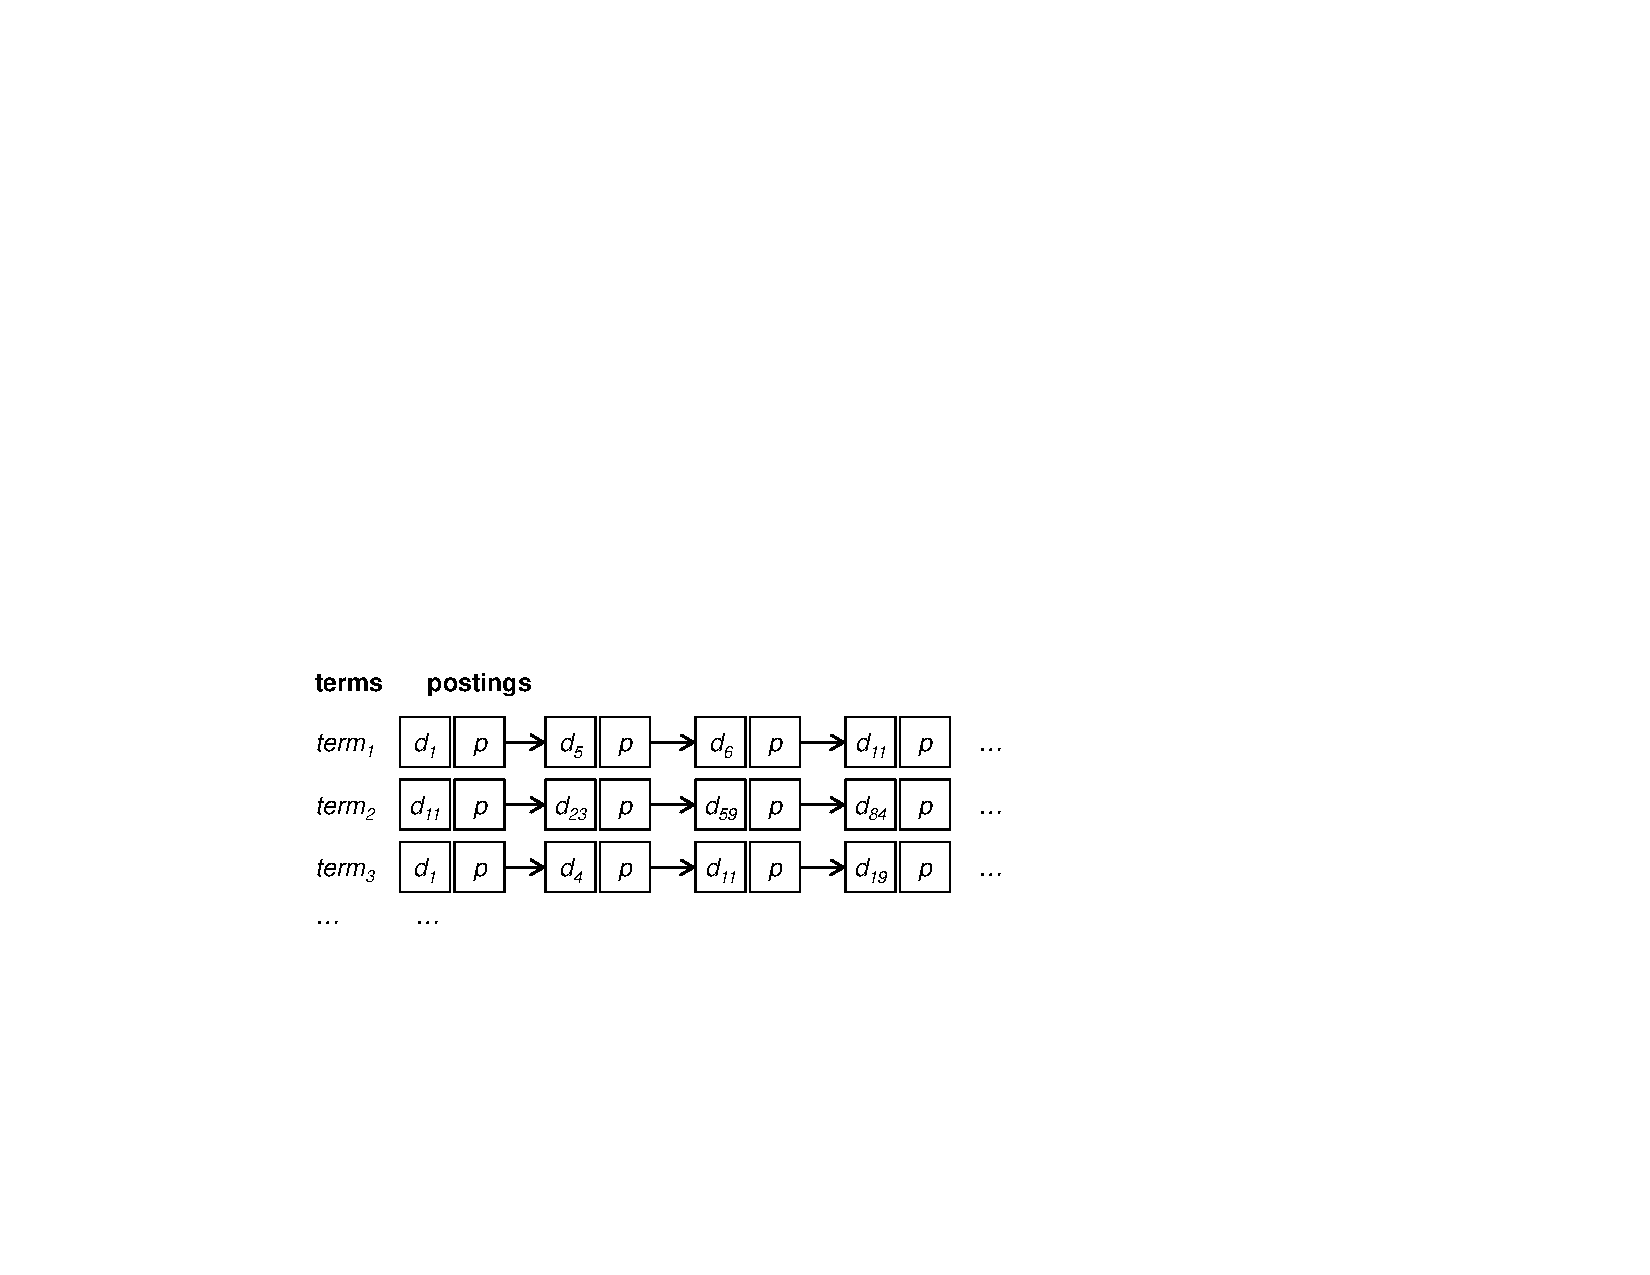
\includegraphics[scale=0.75]{figures/fig-ch4-indexing-inverted-index.pdf}
\vspace{-0.3cm}
\end{center}
\caption{Simple illustration of an inverted index.  Each term is
  associated with a list of postings.  Each posting is comprised of a
  document id and a payload, denoted by \emph{p} in this case.  An
  inverted index provides quick access to documents ids that contain a
  term.}
\label{chapter-indexing:inverted-index}
\end{figure}

In the example shown in Figure~\ref{chapter-indexing:inverted-index},
we see that \emph{term}$_1$ occurs in $\{d_1, d_5, d_6, d_{11},
\ldots\}$, \emph{term}$_2$ occurs in $\{d_{11}, d_{23}, d_{59}, d_{84},
\ldots\}$, and \emph{term}$_3$ occurs in $\{d_1, d_4, d_{11}, d_{19},
\ldots\}$.  In an actual implementation, we assume that documents can
be identified by a unique integer ranging from 1 to \emph{n}, where
\emph{n} is the total number of documents.\footnote{It is preferable to
  start numbering the documents at one since it is not possible to
  code zero with many common compression schemes used in information
  retrieval; see Section~\ref{chapter-indexing:index:compression}.}
Generally, postings are sorted by document id, although other sort
orders are possible as well.  The document ids have no inherent
semantic meaning, although assignment of numeric ids to documents need
not be arbitrary.  For example, pages from the same domain may be
consecutively numbered.  Or, alternatively, pages that are higher in
quality (based, for example, on PageRank values) might be assigned
smaller numeric values so that they appear toward the front of a
postings list.  Either way, an auxiliary data structure is necessary
to maintain the mapping from integer document ids to some other more
meaningful handle, such as a URL.

Given a query, retrieval involves fetching postings lists associated
with query terms and traversing the postings to compute the result
set.  In the simplest case, boolean retrieval involves set operations
(union for boolean OR and intersection for boolean AND) on postings
lists, which can be accomplished very efficiently since the postings
are sorted by document id.  In the general case, however,
query--document scores must be computed.  Partial document scores are
stored in structures called \emph{accumulators}.  At the end (i.e.,
once all postings have been processed), the top \emph{k} documents are
then extracted to yield a ranked list of results for the user.  Of
course, there are many optimization strategies for query evaluation
(both approximate and exact) that reduce the number of postings a
retrieval engine must examine.

The size of an inverted index varies, depending on the payload stored
in each posting.  If only term frequency is stored, a well-optimized
inverted index can be a tenth of the size of the original document
collection.  An inverted index that stores positional information
would easily be several times larger than one that does not.
Generally, it is possible to hold the entire vocabulary (i.e.,
dictionary of all the terms) in memory, especially with techniques
such as front-coding~\cite{Witten_etal_1999}.  However, with the
exception of well-resourced, commercial web search
engines,\footnote{Google keeps indexes in memory.}  postings lists are
usually too large to store in memory and must be held on disk, usually
in compressed form (more details in
Section~\ref{chapter-indexing:index:compression}).  Query evaluation,
therefore, necessarily involves random disk access and ``decoding'' of
the postings.  One important aspect of the retrieval problem is to
organize disk operations such that random seeks are minimized.

Once again, this brief discussion glosses over many complexities and
does a huge injustice to the tremendous amount of research in
information retrieval.  However, our goal is to provide the reader
with an overview of the important issues;
Section~\ref{chapter-indexing:summary} provides references to
additional readings.

\section{Inverted Indexing: Baseline Implementation}
\label{chapter-indexing:index:baseline}

\begin{figure}[t]
\algrenewcommand\algorithmicfunction{\textbf{class}}
  \begin{algorithmic}[1]
    \Function{Mapper}{}
    \Procedure{Map}{$\textrm{docid }n, \textrm{doc }d$}
    \State $H \gets \textrm{new }\textsc{AssociativeArray}$
    \ForAll{$\textrm{term }t \in \textrm{doc }d$}
    \State $H\{t\} \gets H\{t\} + 1$
    \EndFor
    \ForAll{$\textrm{term }t \in H$}
    \State $\textsc{Emit}(\textrm{term }t, \textrm{posting }\langle n, H\{t\} \rangle )$
    \EndFor
    \EndProcedure
    \EndFunction
  \end{algorithmic}

  \begin{algorithmic}[1]
    \Function{Reducer}{}
    \Procedure{Reduce}{$\textrm{term }t, \textrm{postings }[  \langle n_1, f_1 \rangle,  \langle n_2, f_2 \rangle \ldots ]$}
    \State $P \gets \textrm{new }\textsc{List}$
    \ForAll{$\textrm{posting }\langle a, f \rangle \in \textrm{postings }[  \langle n_1, f_1 \rangle,  \langle n_2, f_2 \rangle \ldots ]$}
    \State $\textsc{Append}(P, \langle a, f \rangle )$
    \EndFor
    \State $\textsc{Sort}(P)$
    \State $\textsc{Emit}(\textrm{term }t, \textrm{ postings } P)$
    \EndProcedure
    \EndFunction
  \end{algorithmic}
  \caption{Pseudo-code of the baseline inverted indexing algorithm in
    MapReduce.  Mappers emit postings keyed by terms, the execution
    framework groups postings by term, and the reducers write postings
    lists to disk.}
\label{chapter-indexing:indexing:basic}
\end{figure}

MapReduce was designed from the very beginning to produce the various
data structures involved in web search, including inverted indexes and
the web graph.  We begin with the basic inverted indexing algorithm 
shown in Figure~\ref{chapter-indexing:indexing:basic}.

Input to the mapper consists of document ids (keys) paired with the
actual content (values).  Individual documents are processed in
parallel by the mappers.  First, each document is analyzed and broken
down into its component terms.  The processing pipeline differs
depending on the application and type of document, but for web pages
typically involves stripping out HTML tags and other elements such as
JavaScript code, tokenizing, case folding, removing stopwords (common
words such as `the', `a', `of', etc.), and stemming (removing affixes
from words so that `dogs' becomes `dog').  Once the document has been
analyzed, term frequencies are computed by iterating over all the
terms and keeping track of counts.  Lines 4 and 5 in the pseudo-code
reflect the process of computing term frequencies, but hides the
details of document processing.  After this histogram has been built,
the mapper then iterates over all terms.  For each term, a pair
consisting of the document id and the term frequency is created.  Each
pair, denoted by $\langle n, H\{t\} \rangle$ in the pseudo-code,
represents an individual posting.  The mapper then emits an
intermediate key-value pair with the term as the key and the posting
as the value, in line 7 of the mapper pseudo-code.  Although as
presented here only the term frequency is stored in the posting, this
algorithm can be easily augmented to store additional information
(e.g., term positions) in the payload.

In the shuffle and sort phase, the MapReduce runtime essentially
performs a large, distributed group by of the postings by term.
Without any additional effort by the programmer, the execution
framework brings together all the postings that belong in the same
postings list.  This tremendously simplifies the task of the reducer,
which simply needs to gather together all the postings and write them
to disk.  The reducer begins by initializing an empty list and then
appends all postings associated with the same key (term) to the list.
The postings are then sorted by document id, and the entire postings
list is emitted as a value, with the term as the key.  Typically, the
postings list is first compressed, but we leave this aside for now
(see Section~\ref{chapter-indexing:index:revised} for more details).
The final key-value pairs are written to disk and comprise the
inverted index.  Since each reducer writes its output in a separate
file in the distributed file system, our final index will be split
across $r$ files, where $r$ is the number of reducers.  There is no
need to further consolidate these files.  Separately, we must also
build an index to the postings lists themselves for the retrieval
engine:\ this is typically in the form of mappings from term to (file,
byte offset) pairs, so that given a term, the retrieval engine can
fetch its postings list by opening the appropriate file and seeking to
the correct byte offset position in that file.

\begin{figure}[t]
\begin{center}
\vspace{0.2cm}
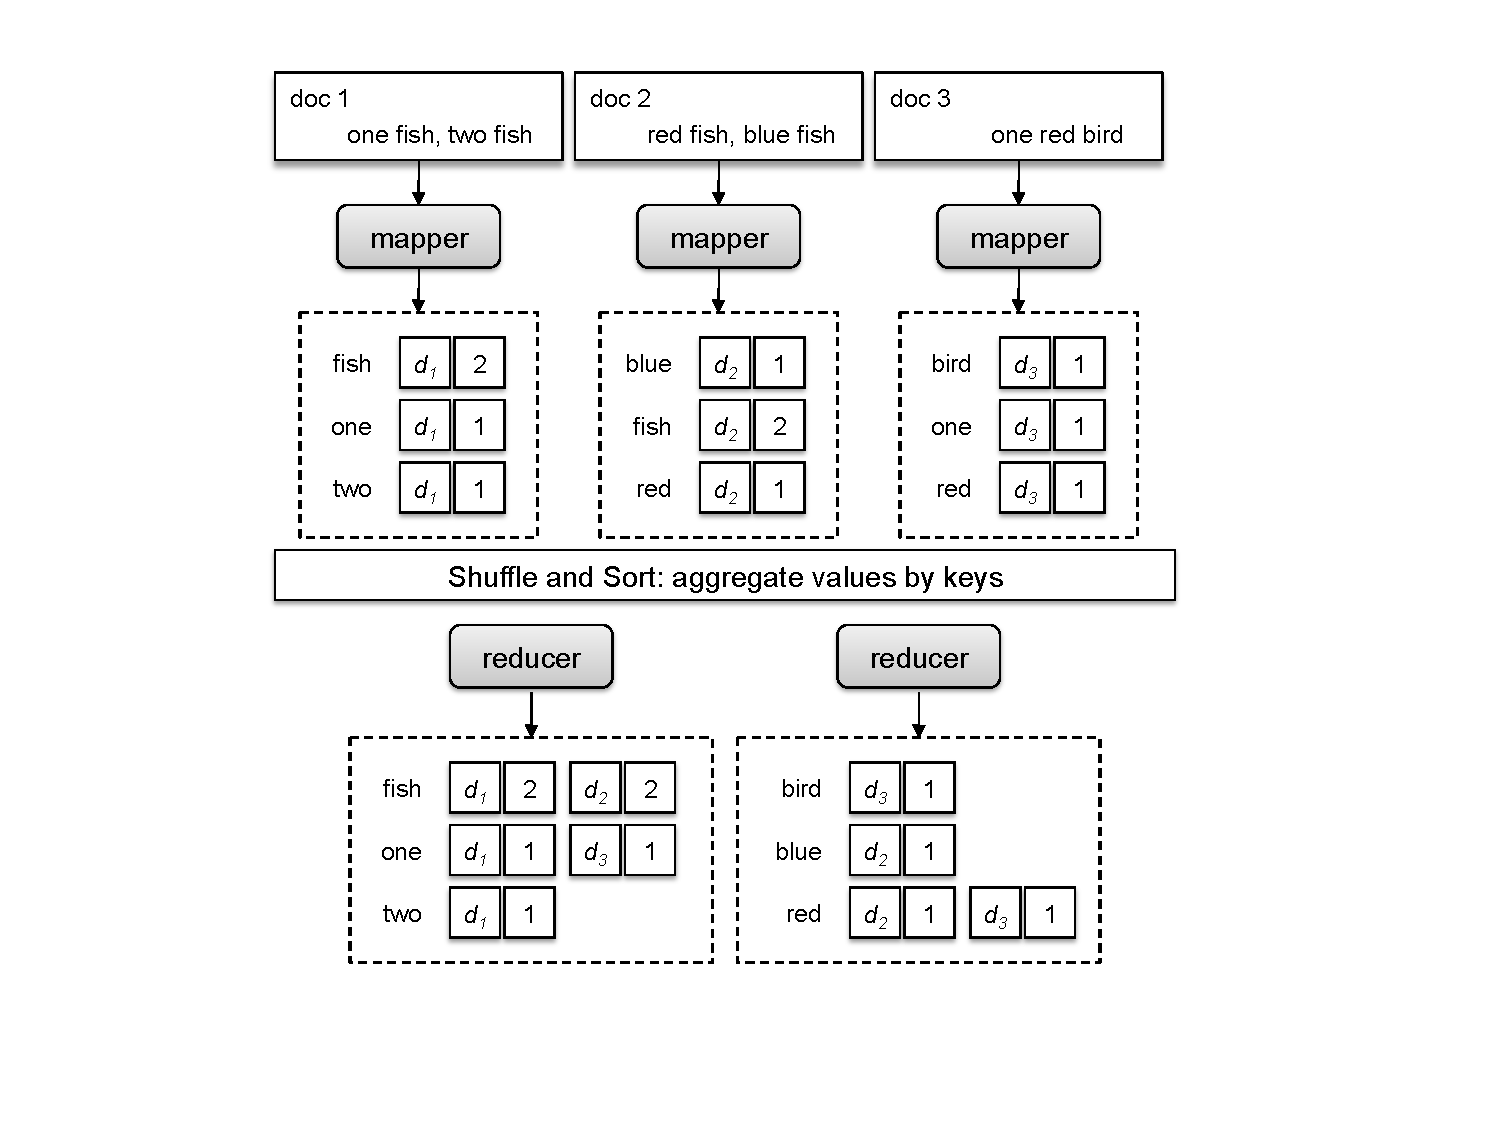
\includegraphics[scale=0.6]{figures/fig-ch4-indexing-MR-baseline.pdf}
\vspace{-0.3cm}
\end{center}
\caption{Simple illustration of the baseline inverted indexing
  algorithm in MapReduce with three mappers and two reducers.
  Postings are shown as pairs of boxes (\emph{docid}, \emph{tf}).}
\label{chapter-indexing:MR-baseline}
\end{figure}

Execution of the complete algorithm is illustrated in
Figure~\ref{chapter-indexing:MR-baseline} with a toy example
consisting of three documents, three mappers, and two reducers.
Intermediate key-value pairs (from the mappers) and the final
key-value pairs comprising the inverted index (from the reducers) are
shown in the boxes with dotted lines.  Postings are shown as pairs of
boxes, with the document id on the left and the term frequency on the
right.

The MapReduce programming model provides a very concise expression of
the inverted indexing algorithm.  Its implementation is similarly
concise:\ the basic algorithm can be implemented in as few as a couple
dozen lines of code in Hadoop (with minimal document processing).
Such an implementation can be completed as a week-long programming
assignment in a course for advanced undergraduates or first-year
graduate students~\cite{KimballA_etal_2008,Lin_TeachCL2008}.  In a
non-MapReduce indexer, a significant fraction of the code is devoted
to grouping postings by term, given constraints imposed by memory and
disk (e.g., memory capacity is limited, disk seeks are slow, etc.).
In MapReduce, the programmer does not need to worry about any of these
issues---most of the heavy lifting is performed by the execution
framework.

\section{Inverted Indexing: Revised Implementation}
\label{chapter-indexing:index:revised}

The inverted indexing algorithm presented in the previous section
serves as a reasonable baseline.  However, there is a significant
scalability bottleneck:\ the algorithm assumes that there is
sufficient memory to hold all postings associated with the same term.
Since the basic MapReduce execution framework makes no guarantees
about the ordering of values associated with the same key, the reducer
first buffers all postings (line 5 of the reducer pseudo-code in
Figure~\ref{chapter-indexing:indexing:basic}) and then performs an
in-memory sort before writing the postings to disk.\footnote{See
  similar discussion in Section~\ref{chapter3:secondary-sorting}:\ in
  principle, this need not be an in-memory sort.  It is entirely
  possible to implement a disk-based sort within the reducer.}  For
efficient retrieval, postings need to be sorted by document id.
However, as collections become larger, postings lists grow longer, and
at some point in time, reducers will run out of memory.

There is a simple solution to this problem.  Since the execution
framework guarantees that keys arrive at each reducer in sorted order,
one way to overcome the scalability bottleneck is to let the MapReduce
runtime do the sorting for us.  Instead of emitting key-value pairs of
the following type:

\begin{quote}
$(\textrm{term }t, \textrm{posting }\langle docid, f \rangle )$
\end{quote}

\noindent We emit intermediate key-value pairs of the type instead:

\begin{quote}
$(\textrm{tuple }\langle t, docid \rangle, \textrm{tf }f )$
\end{quote}

\noindent In other words, the key is a tuple containing the term and
the document id, while the value is the term frequency.  This is
exactly the value-to-key conversion design pattern introduced in
Section~\ref{chapter3:secondary-sorting}.  With this modification, the
programming model ensures that the postings arrive in the correct
order.  This, combined with the fact that reducers can hold state
across multiple keys, allows postings lists to be created with minimal
memory usage.  As a detail, remember that we must define a custom
partitioner to ensure that all tuples with the same term are shuffled
to the same reducer.

The revised MapReduce inverted indexing algorithm is shown in
Figure~\ref{chapter-indexing:scalable}.  The mapper remains unchanged
for the most part, other than differences in the intermediate
key-value pairs.  The \textsc{Reduce} method is called for each key
(i.e., $\langle t, n \rangle$), and by design, there will only be one
value associated with each key.  For each key-value pair, a posting
can be directly added to the postings list.  Since the postings are
guaranteed to arrive in sorted order by document id, they can be
incrementally coded in compressed form---thus ensuring a small
memory footprint.  Finally, when all postings associated with the same
term have been processed (i.e., $t \ne t_{prev}$), the entire postings
list is emitted.  The final postings list must be written out in the
\textsc{Close} method.  As with the baseline algorithm, payloads can
be easily changed:\ by simply replacing the intermediate value $f$
(term frequency) with whatever else is desired (e.g., term positional
information).

\begin{figure}[t]
\algrenewcommand\algorithmicfunction{\textbf{class}}
\algrenewcommand\algorithmicprocedure{\textbf{method}}
  \begin{algorithmic}[1]
    \Function{Mapper}{}
    \Procedure{Map}{$\textrm{docid }n, \textrm{doc }d$}
    \State $H \gets \textrm{new }\textsc{AssociativeArray}$
    \ForAll{$\textrm{term }t \in \textrm{doc }d$}
    \State $H\{t\} \gets H\{t\} + 1$
    \EndFor
    \ForAll{$\textrm{term }t \in H$}
    \State $\textsc{Emit}(\textrm{tuple }\langle t, n \rangle, \textrm{tf }H\{t\} )$
    \EndFor
    \EndProcedure
    \EndFunction
  \end{algorithmic}

  \begin{algorithmic}[1]
    \Function{Reducer}{}
    \Procedure{Initialize}{}
      \State $t_{prev} \gets \emptyset$
      \State $P \gets \textrm{new }\textsc{PostingsList}$
    \EndProcedure
    \Procedure{Reduce}{$\textrm{tuple }\langle t, n \rangle, \textrm{tf }[ f ]$}
    \If{$t \ne t_{prev} \land t_{prev} \ne \emptyset$}
      \State $\textsc{Emit}(\textrm{term }t, \textrm{ postings } P)$
      \State $P.\textsc{{\small Reset}}()$
    \EndIf
    \State $P.\textsc{{\small Add}}(\langle n, f \rangle)$
    \State $t_{prev} \gets t$
    \EndProcedure
    \Procedure{Close}{}
      \State $\textsc{Emit}(\textrm{term }t, \textrm{ postings } P)$
    \EndProcedure
    \EndFunction
  \end{algorithmic}
  \caption{Pseudo-code of a scalable inverted indexing algorithm in
    MapReduce.  By applying the value-to-key conversion design
    pattern, the execution framework is exploited to sort postings so
    that they arrive sorted by document id in the reducer.}
\label{chapter-indexing:scalable}
\end{figure}

There is one more detail we must address when building inverted
indexes.  Since almost all retrieval models take into account document
length when computing query--document scores, this information must
also be extracted.  Although it is straightforward to express this
computation as another MapReduce job, this task can actually be folded
into the inverted indexing process.  When processing the terms in each
document, the document length is known, and can be written out as
``side data'' directly to HDFS.  We can take advantage of the ability
for a mapper to hold state across the processing of multiple documents
in the following manner:\ an in-memory associative array is created to
store document lengths, which is populated as each document is
processed.\footnote{In general, there is no worry about insufficient
  memory to hold these data.}  When the mapper finishes processing
input records, document lengths are written out to HDFS (i.e., in the
\textsc{Close} method).  This approach is essentially a variant of the
in-mapper combining pattern.  Document length data ends up in $m$
different files, where $m$ is the number of mappers; these files are
then consolidated into a more compact representation.  Alternatively,
document length information can be emitted in special key-value pairs
by the mapper.  One must then write a custom partitioner so that these
special key-value pairs are shuffled to a single reducer, which will
be responsible for writing out the length data separate from the
postings lists.

\section{Index Compression}
\label{chapter-indexing:index:compression}

We return to the question of how postings are actually compressed and
stored on disk.  This chapter devotes a substantial amount of space to
this topic because index compression is one of the main differences
between a ``toy'' indexer and one that works on real-world
collections.  Otherwise, MapReduce inverted indexing algorithms are
pretty straightforward.

Let us consider the canonical case where each posting consists of a
document id and the term frequency.  A na\"ive implementation might
represent the first as a 32-bit integer\footnote{However, note that
  $2^{32}-1$ is ``only'' 4,294,967,295, which is much less than even
  the most conservative estimate of the size of the web.} and the
second as a 16-bit integer.  Thus, a postings list might be encoded as
follows:

\begin{quote}
$[ (5, 2), (7, 3), (12, 1), (49, 1), (51, 2), \ldots]$
\end{quote}

\noindent where each posting is represented by a pair in parentheses.
Note that all brackets, parentheses, and commas are only included to
enhance readability; in reality the postings would be represented as a
long stream of integers.  This na\"ive implementation would require
six bytes per posting.  Using this scheme, the entire inverted index
would be about as large as the collection itself.  Fortunately, we can
do significantly better.

The first trick is to encode \emph{differences} between document ids as
opposed to the document ids themselves.  Since the postings are sorted
by document ids, the differences (called \emph{d}-gaps) must be
positive integers greater than zero.  The above postings list,
represented with \emph{d}-gaps, would be:

\begin{quote}
$[ (5, 2), (2, 3), (5, 1), (37, 1), (2, 2), \ldots]$
\end{quote}

\noindent Of course, we must actually encode the first document id.
We haven't lost any information, since the original document ids can
be easily reconstructed from the \emph{d}-gaps.  However, it's not
obvious that we've reduced the space requirements either, since the
largest possible \emph{d}-gap is one less than the number of documents
in the collection.

This is where the second trick comes in, which is to represent the
\emph{d}-gaps in a way such that it takes less space for smaller
numbers.  Similarly, we want to apply the same techniques to compress
the term frequencies, since for the most part they are also small
values.  But to understand how this is done, we need to take a slight
detour into compression techniques, particularly for coding integers.

Compression, in general, can be characterized as either \emph{lossless}
or \emph{lossy}:\ it's fairly obvious that loseless compression is
required in this context.  To start, it is important to understand
that all compression techniques represent a time--space tradeoff.
That is, we reduce the amount of space on disk necessary to store
data, but at the cost of extra processor cycles that must be spent
coding and decoding data.  Therefore, it is possible that compression
reduces size but also slows processing.  However, if the two factors
are properly balanced (i.e., decoding speed can keep up with disk
bandwidth), we can achieve the best of both worlds:\ smaller \emph{and}
faster.

\subsection{Byte-Aligned and Word-Aligned Codes}

In most programming languages, an integer is encoded in four bytes and
holds a value between 0 and $2^{32}-1$, inclusive. We limit our
discussion to \emph{unsigned} integers, since \emph{d}-gaps are always
positive (and greater than zero).  This means that 1 and 4,294,967,295
both occupy four bytes.  Obviously, encoding \emph{d}-gaps this way
doesn't yield any reductions in size.

A simple approach to compression is to only use as many bytes as is
necessary to represent the integer.  This is known as variable-length
integer coding (varInt for short) and accomplished by using the high
order bit of every byte as the \emph{continuation bit}, which is set to
one in the last byte and zero elsewhere.  As a result, we have 7 bits
per byte for coding the value, which means that $0 \leq n < 2^7$ can
be expressed with 1 byte, $2^{7} \leq n < 2^{14}$ with 2 bytes,
$2^{14} \leq n < 2^{21}$ with 3, and $2^{21} \leq n < 2^{28}$ with 4
bytes.  This scheme can be extended to code arbitrarily-large integers
(i.e., beyond 4 bytes).  As a concrete example, the two numbers:

\begin{quote}
127, 128
\end{quote}

\noindent would be coded as such:

\begin{quote}
1 1111111, 0 0000001 1 0000000
\end{quote}

\noindent The above code contains two code words, the first consisting
of 1 byte, and the second consisting of 2 bytes.  Of course, the comma
and the spaces are there only for readability.  Variable-length
integers are byte-aligned because the code words always fall along
byte boundaries.  As a result, there is never any ambiguity about
where one code word ends and the next begins.  However, the downside
of varInt coding is that decoding involves lots of bit operations
(masks, shifts).  Furthermore, the continuation bit sometimes results
in frequent branch mispredicts (depending on the actual distribution
of \emph{d}-gaps), which slows down processing.

A variant of the varInt scheme was described by Jeff Dean in a keynote
talk at the WSDM 2009 conference.\footnote{\texttt{
  http://research.google.com/people/jeff/WSDM09-keynote.pdf}} The
insight is to code groups of four integers at a time.  Each group
begins with a prefix byte, divided into four 2-bit values that specify
the byte length of each of the following integers.  For example, the
following prefix byte:

\begin{quote}
00,00,01,10
\end{quote}

\noindent indicates that the following four integers are one byte, one
byte, two bytes, and three bytes, respectively.  Therefore, each group
of four integers would consume anywhere between 5 and 17 bytes.  A
simple lookup table based on the prefix byte directs the decoder on
how to process subsequent bytes to recover the coded integers.  The
advantage of this group varInt coding scheme is that values can be
decoded with fewer branch mispredicts and bitwise operations.
Experiments reported by Dean suggest that decoding integers with this
scheme is more than twice as fast as the basic varInt scheme.

In most architectures, accessing entire machine words is more
efficient than fetching all its bytes separately.  Therefore, it makes
sense to store postings in increments of 16-bit, 32-bit, or 64-bit
machine words.  Anh and Moffat~\cite{Anh_Moffat_2005} presented
several word-aligned coding methods, one of which is called Simple-9,
based on 32-bit words.  In this coding scheme, four bits in each
32-bit word are reserved as a \emph{selector}.  The remaining 28 bits
are used to code actual integer values.  Now, there are a variety of
ways these 28 bits can be divided to code one or more integers:\ 28
bits can be used to code one 28-bit integer, two 14-bit integers,
three 9-bit integers (with one bit unused), etc., all the way up to
twenty-eight 1-bit integers.  In fact, there are nine different ways
the 28 bits can be divided into equal parts (hence the name of the
technique), some with leftover unused bits.  This is stored in the
selector bits.  Therefore, decoding involves reading a 32-bit word,
examining the selector to see how the remaining 28 bits are packed,
and then appropriately decoding each integer.  Coding works in the
opposite way:\ the algorithm scans ahead to see how many integers can
be squeezed into 28 bits, packs those integers, and sets the selector
bits appropriately.

\subsection{Bit-Aligned Codes}

The advantage of byte-aligned and word-aligned codes is that they can
be coded and decoded quickly.  The downside, however, is that they
\emph{must} consume multiples of eight bits, even when fewer bits might
suffice (the Simple-9 scheme gets around this by packing multiple
integers into a 32-bit word, but even then, bits are often wasted).
In bit-aligned codes, on the other hand, code words can occupy any
number of bits, meaning that boundaries can fall anywhere.  In
practice, coding and decoding bit-aligned codes require processing
bytes and appropriately shifting or masking bits (usually more
involved than varInt and group varInt coding).

One additional challenge with bit-aligned codes is that we need a
mechanism to delimit code words, i.e., tell where the last ends and
the next begins, since there are no byte boundaries to guide us.  To
address this issue, most bit-aligned codes are so-called prefix codes
(confusingly, they are also called prefix-free codes), in which no
valid code word is a prefix of any other valid code word.  For
example, coding $0 \leq x < 3$ with $\{0, 1, 01\}$ is not a valid
prefix code, since 0 is a prefix of 01, and so we can't tell if 01 is
two code words or one.  On the other hand, $\{00, 01, 1\}$ is a valid
prefix code, such that a sequence of bits:

\begin{quote}
0001101001010100
\end{quote}

\noindent can be unambiguously segmented into:

\begin{quote}
00 01 1 01 00 1 01 01 00
\end{quote}

\noindent and decoded without any additional delimiters.

One of the simplest prefix codes is the unary code.  An integer $x>0$
is coded as $x-1$ one bits followed by a zero bit.  Note that unary
codes do not allow the representation of zero, which is fine since
\emph{d}-gaps and term frequencies should never be zero.\footnote{As a
  note, some sources describe slightly different formulations of the
  same coding scheme.  Here, we adopt the conventions used in the
  classic IR text \emph{Managing Gigabytes}~\cite{Witten_etal_1999}.}
As an example, 4 in unary code is 1110.  With unary code we can code
$x$ in $x$ bits, which although economical for small values, becomes
inefficient for even moderately large values.  Unary codes are rarely
used by themselves, but form a component of other coding schemes.
Unary codes of the first ten positive integers are shown in
Figure~\ref{chapter-indexing:encoding-schemes}.

\begin{figure}[t]
\centering
\begin{tabular}{lllll}
\hline
    &       &          & Golomb \\
$x$ & unary & $\gamma$ & $b=5$ & $b=10$\\
\hline
1  & 0          & 0        & 0:00   & 0:000\\
2  & 10         & 10:0     & 0:01   & 0:001\\
3  & 110        & 10:1     & 0:10   & 0:010\\
4  & 1110       & 110:00   & 0:110  & 0:011\\
5  & 11110      & 110:01   & 0:111  & 0:100\\
6  & 111110     & 110:10   & 10:00  & 0:101\\
7  & 1111110    & 110:11   & 10:01  & 0:1100\\
8  & 11111110   & 1110:000 & 10:10  & 0:1101\\
9  & 111111110  & 1110:001 & 10:110 & 0:1110\\
10 & 1111111110 & 1110:010 & 10:111 & 0:1111\\
\hline
\end{tabular}
\caption{The first ten positive integers in unary, $\gamma$, and
  Golomb ($b=5,10$) codes.}
\label{chapter-indexing:encoding-schemes}
\end{figure}

Elias $\gamma$ code is an efficient coding scheme that is widely used
in practice.  An integer $x>0$ is broken into two components, $1 +
\lfloor \log_2 x \rfloor$ ($=n$, the length), which is coded in unary
code, and $x-2^{\lfloor \log_2 x \rfloor}$ ($=r$, the remainder),
which is in binary.\footnote{Note that $\lfloor x \rfloor$ is the
  floor function, which maps $x$ to the largest integer not greater
  than $x$, so, e.g., $\lfloor 3.8 \rfloor = 3$. This is the default
  behavior in many programming languages when casting from a
  floating-point type to an integer type.}  The unary component $n$
specifies the number of bits required to code $x$, and the binary
component codes the remainder $r$ in $n-1$ bits.  As an example,
consider $x=10$: $1 + \lfloor \log_2 10 \rfloor = 4$, which is 1110.
The binary component codes $x-2^3=2$ in $4-1=3$ bits, which is 010.
Putting both together, we arrive at 1110:010. The extra colon is
inserted only for readability; it's not part of the final code, of
course.

Working in reverse, it is easy to unambiguously decode a bit stream of
$\gamma$ codes: First, we read a unary code $c_u$, which is a prefix
code.  This tells us that the binary portion is written in $c_u-1$
bits, which we then read as $c_b$.  We can then reconstruct $x$ as
$2^{c_u-1} + c_b$.  For $x<16$, $\gamma$ codes occupy less than a full
byte, which makes them more compact than variable-length integer
codes.  Since term frequencies for the most part are relatively small,
$\gamma$ codes make sense for them and can yield substantial space
savings.  For reference, the $\gamma$ codes of the first ten positive
integers are shown in Figure~\ref{chapter-indexing:encoding-schemes}.
A variation on $\gamma$ code is $\delta$ code, where the $n$ portion
of the $\gamma$ code is coded in $\gamma$ code itself (as opposed to
unary code).  For smaller values $\gamma$ codes are more compact, but
for larger values, $\delta$ codes take less space.

Unary and $\gamma$ codes are parameterless, but even better
compression can be achieved with parameterized codes.  A good example
of this is Golomb code.  For some parameter $b$, an integer $x>0$ is
coded in two parts:\ first, we compute $q = \lfloor (x-1)/b \rfloor$
and code $q+1$ in unary; then, we code the remainder $r = x - qb -1$
in truncated binary.  This is accomplished as follows:\ if $b$ is a
power of two, then truncated binary is exactly the same as normal
binary, requiring $\log_2 b$ bits.  Otherwise, we code the first
$2^{\lfloor \log_2 b \rfloor+1} - b$ values of $r$ in $\lfloor \log_2
b \rfloor$ bits and code the rest of the values of $r$ by coding
$r+2^{\lfloor \log_2 b \rfloor+1} - b$ in ordinary binary
representation using $\lfloor \log_2 b \rfloor+1$ bits.  In this case,
the $r$ is coded in either $\lfloor \log_2 b \rfloor$ or $\lfloor
\log_2 b \rfloor +1$ bits, and unlike ordinary binary coding,
truncated binary codes are prefix codes.  As an example, if $b=5$,
then $r$ can take the values $\{0, 1, 2, 3, 4\}$, which would be coded
with the following code words: $\{00,01,10,110,111\}$.  For reference,
Golomb codes of the first ten positive integers are shown in
Figure~\ref{chapter-indexing:encoding-schemes} for $b=5$ and $b=10$.
A special case of Golomb code is worth noting:\ if $b$ is a power of
two, then coding and decoding can be handled more efficiently (needing
only bit shifts and bit masks, as opposed to multiplication and
division).  These are known as Rice codes.

Researchers have shown that Golomb compression works well for \emph{
  d}-gaps, and is optimal with the following parameter setting:

\begin{equation}
b \approx 0.69 \times \frac{df}{N}
\end{equation}

\noindent where $df$ is the document frequency of the term, and $N$ is
the number of documents in the collection.\footnote{For details as to
  why this is the case, we refer the reader
  elsewhere~\cite{Witten_etal_1999}, but here's the intuition:\ under
  reasonable assumptions, the appearance of postings can be modeled as
  a sequence of independent Bernoulli trials, which implies a certain
  distribution of \emph{d}-gaps.  From this we can derive an optimal
  setting of $b$.}

Putting everything together, one popular approach for postings
compression is to represent \emph{d}-gaps with Golomb codes and term
frequencies with $\gamma$
codes~\cite{Witten_etal_1999,Zobel_Moffat_2006}.  If positional
information is desired, we can use the same trick to code differences
between term positions using $\gamma$ codes.

\subsection{Postings Compression}

Having completed our slight detour into integer compression
techniques, we can now return to the scalable inverted indexing
algorithm shown in Figure~\ref{chapter-indexing:scalable} and discuss
how postings lists can be properly compressed.  As we can see from the
previous section, there is a wide range of choices that represent
different tradeoffs between compression ratio and decoding speed.
Actual performance also depends on characteristics of the collection,
which, among other factors, determine the distribution of \emph{
  d}-gaps.  B\"uttcher et al.~\cite{Buttcher_etal_2010} recently
compared the performance of various compression techniques on coding
document ids.  In terms of the amount of compression that can be
obtained (measured in bits per \emph{docid}), Golomb and Rice codes
performed the best, followed by $\gamma$ codes, Simple-9, varInt, and
group varInt (the least space efficient).  In terms of raw decoding
speed, the order was almost the reverse:\ group varInt was the
fastest, followed by varInt.\footnote{However, this study found less
  speed difference between group varInt and basic varInt than Dean's
  analysis, presumably due to the different distribution of \emph{d}-gaps
  in the collections they were examining.}  Simple-9 was substantially
slower, and the bit-aligned codes were even slower than that.  Within
the bit-aligned codes, Rice codes were the fastest, followed by
$\gamma$, with Golomb codes being the slowest (about ten times slower
than group varInt).

Let us discuss what modifications are necessary to our inverted
indexing algorithm if we were to adopt Golomb compression for \emph{
  d}-gaps and represent term frequencies with $\gamma$ codes.  Note
that this represents a space-efficient encoding, at the cost of slower
decoding compared to alternatives.  Whether or not this is actually a
worthwhile tradeoff in practice is not important here:\ use of Golomb
codes serves a pedagogical purpose, to illustrate how one might set
compression parameters.

Coding term frequencies with $\gamma$ codes is easy since they are
parameterless.  Compressing \emph{d}-gaps with Golomb codes, however,
is a bit tricky, since two parameters are required:\ the size of the
document collection and the number of postings for a particular
postings list (i.e., the document frequency, or \emph{df}).  The first
is easy to obtain and can be passed into the reducer as a constant.
The \emph{df} of a term, however, is not known until all the postings
have been processed---and unfortunately, the parameter must be known
before any posting is coded.  At first glance, this seems like a
chicken-and-egg problem.  A two-pass solution that involves first
buffering the postings (in memory) would suffer from the memory
bottleneck we've been trying to avoid in the first place.

To get around this problem, we need to somehow inform the reducer of a
term's \emph{df} before any of its postings arrive.  This can be solved
with the order inversion design pattern introduced in
Section~\ref{chapter3:cond-prob} to compute relative frequencies.  The
solution is to have the mapper emit special keys of the form $\langle
t, \ast \rangle$ to communicate partial document frequencies.  That
is, inside the mapper, in addition to emitting intermediate key-value
pairs of the following form:

\begin{quote}
$(\textrm{tuple }\langle t, docid \rangle, \textrm{tf }f )$
\end{quote}

\noindent we also emit special intermediate key-value pairs like this:

\begin{quote}
$(\textrm{tuple }\langle t, \ast \rangle, \textrm{df }e )$
\end{quote}

\noindent to keep track of document frequencies associated with each
term.  In practice, we can accomplish this by applying the in-mapper
combining design pattern (see
Section~\ref{chapter3:local-aggregation}).  The mapper holds an
in-memory associative array that keeps track of how many documents a
term has been observed in (i.e., the local document frequency of the
term for the subset of documents processed by the mapper).  Once the
mapper has processed all input records, special keys of the form
$\langle t, \ast \rangle$ are emitted with the partial \emph{df} as the
value.

To ensure that these special keys arrive first, we define the sort
order of the tuple so that the special symbol $\ast$ precedes all
documents (part of the order inversion design pattern).  Thus, for
each term, the reducer will first encounter the $\langle t, \ast
\rangle$ key, associated with a list of values representing partial
       \emph{df} values originating from each mapper.  Summing all
       these partial contributions will yield the term's \emph{df},
       which can then be used to set the Golomb compression parameter
       $b$.  This allows the postings to be incrementally compressed
       as they are encountered in the reducer---memory bottlenecks are
       eliminated since we do not need to buffer postings in memory.

Once again, the order inversion design pattern comes to the rescue.
Recall that the pattern is useful when a reducer needs to access the
result of a computation (e.g., an aggregate statistic) before it
encounters the data necessary to produce that computation.  For
computing relative frequencies, that bit of information was the
marginal.  In this case, it's the document frequency.

\section{What About Retrieval?}
\label{chapter-indexing:retrieval}

Thus far, we have briefly discussed web crawling and focused mostly on
MapReduce algorithms for inverted indexing.  What about retrieval?  It
should be fairly obvious that MapReduce, which was designed for large
batch operations, is a poor solution for retrieval.  Since users
demand sub-second response times, every aspect of retrieval must be
optimized for low latency, which is exactly the opposite tradeoff made
in MapReduce.  Recall the basic retrieval problem:\ we must look up
postings lists corresponding to query terms, systematically traverse
those postings lists to compute query--document scores, and then
return the top $k$ results to the user.  Looking up postings implies
random disk seeks, since for the most part postings are too large to
fit into memory (leaving aside caching and other special cases for
now).  Unfortunately, random access is not a forte of the distributed
file system underlying MapReduce---such operations require multiple
round-trip network exchanges (and associated latencies).  In HDFS, a
client must first obtain the location of the desired data block from
the namenode before the appropriate datanode can be contacted for the
actual data.  Of course, access will typically require a random disk
seek on the datanode itself.

It should be fairly obvious that serving the search needs of a large
number of users, each of whom demand sub-second response times, is
beyond the capabilities of any single machine.  The only solution is
to distribute retrieval across a large number of machines, which
necessitates breaking up the index in some manner.  There are two main
partitioning strategies for distributed retrieval:\ \emph{document
  partitioning} and \emph{term partitioning}.  Under document
partitioning, the entire collection is broken up into multiple smaller
sub-collections, each of which is assigned to a server.  In other
words, each server holds the complete index for a subset of the entire
collection.  This corresponds to partitioning vertically in
Figure~\ref{chapter-indexing:partition}.  With term partitioning, on
the other hand, each server is responsible for a subset of the terms
for the entire collection.  That is, a server holds the postings for
all documents in the collection for a subset of terms.  This
corresponds to partitioning horizontally in
Figure~\ref{chapter-indexing:partition}.

\begin{figure}[t]
\begin{center}
\vspace{0.2cm}
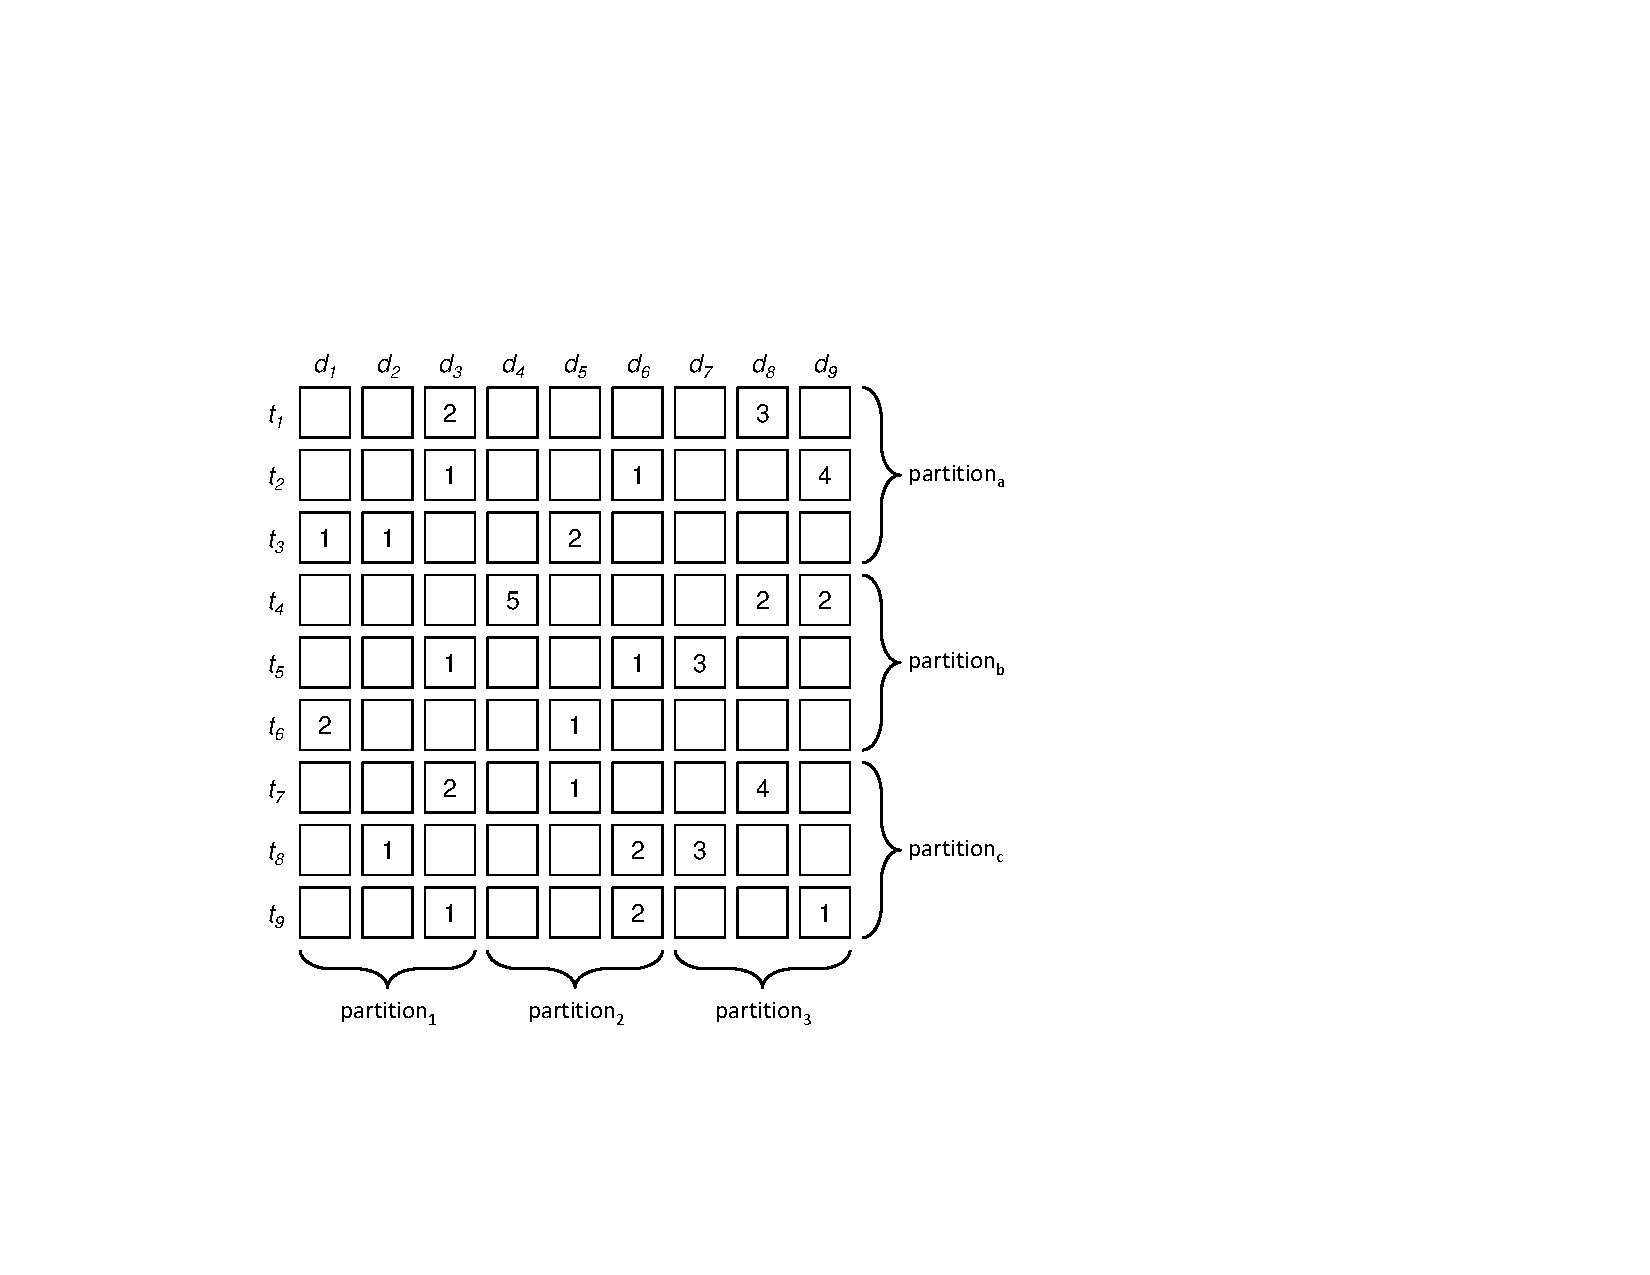
\includegraphics[scale=0.75]{figures/fig-ch4-indexing-partition.pdf}
\vspace{-0.3cm}
\end{center}
\caption{Term--document matrix for a toy collection (nine documents,
  nine terms) illustrating different partitioning
  strategies:\ partitioning vertically ($1,2,3$) corresponds to
  document partitioning, whereas partitioning horizontally ($a,b,c$)
  corresponds to term partitioning.}
\label{chapter-indexing:partition}
\end{figure}

Document and term partitioning require different retrieval strategies
and represent different tradeoffs.  Retrieval under document
partitioning involves a query broker, which forwards the user's query
to all partition servers, merges partial results from each, and then
returns the final results to the user.  With this architecture,
searching the entire collection requires that the query be processed
by every partition server.  However, since each partition operates
independently and traverses postings in parallel, document
partitioning typically yields shorter query latencies (compared to a
single monolithic index with much longer postings lists).  

Retrieval under term partitioning, on the other hand, requires a very
different strategy.  Suppose the user's query $Q$ contains three
terms, $q_1$, $q_2$, and $q_3$.  Under the pipelined query evaluation
strategy, the broker begins by forwarding the query to the server that
holds the postings for $q_1$ (usually the least frequent term).  The
server traverses the appropriate postings list and computes partial
query--document scores, stored in the accumulators.  The accumulators
are then passed to the server that holds the postings associated with
$q_2$ for additional processing, and then to the server for $q_3$,
before final results are passed back to the broker and returned to the
user.  Although this query evaluation strategy may not substantially
reduce the latency of any particular query, it can theoretically
increase a system's throughput due to the far smaller number of total
disk seeks required for each user query (compared to document
partitioning).  However, load-balancing is tricky in a pipelined
term-partitioned architecture due to skew in the distribution of query
terms, which can create ``hot spots'' on servers that hold the
postings for frequently-occurring query terms.

In general, studies have shown that document partitioning is a better
strategy overall~\cite{Moffat_etal_SIGIR2006}, and this is the
strategy adopted by Google~\cite{Barroso03}.  Furthermore, it is known
that Google maintains its indexes in memory (although this is
certainly not the common case for search engines in general).  One key
advantage of document partitioning is that result quality degrades
gracefully with machine failures.  Partition servers that are offline
will simply fail to deliver results for their subsets of the
collection.  With sufficient partitions, users might not even be aware
that documents are missing.  For most queries, the web contains
more relevant documents than any user has time to digest:\ users of
course care about getting relevant documents (sometimes, they are
happy with a single relevant document), but they are generally less
discriminating when it comes to \emph{which} relevant documents appear
in their results (out of the set of \emph{all} relevant documents).
Note that partitions may be unavailable due to reasons other than
machine failure:\ cycling through different partitions is a very
simple and non-disruptive strategy for index updates.

Working in a document-partitioned architecture, there are a variety of
approaches to dividing up the web into smaller pieces.  Proper
partitioning of the collection can address one major weakness of this
architecture, which is that every partition server is involved in
every user query.  Along one dimension, it is desirable to partition
by document quality using one or more classifiers; see~\cite{qiACS09}
for a recent survey on web page classification.  Partitioning by
document quality supports a multi-phase search strategy:\ the system
examines partitions containing high quality documents first, and only
backs off to partitions containing lower quality documents if
necessary.  This reduces the number of servers that need to be
contacted for a user query.  Along an orthogonal dimension, it is
desirable to partition documents by content (perhaps also guided by
the distribution of user queries from logs), so that each partition is
``well separated'' from the others in terms of topical
coverage.  This also reduces the number of machines that need
to be involved in serving a user's query:\ the broker can direct
queries only to the partitions that are likely to contain relevant
documents, as opposed to forwarding the user query to all the
partitions.

On a large-scale, reliability of service is provided by replication,
both in terms of multiple machines serving the same partition within a
single datacenter, but also replication across
geographically-distributed datacenters.  This creates at least two
query routing problems:\ since it makes sense to serve clients from
the closest datacenter, a service must route queries to the
appropriate location.  Within a single datacenter, the system needs to
properly balance load across replicas.

There are two final components of real-world search engines that are
worth discussing.  First, recall that postings only store document
ids.  Therefore, raw retrieval results consist of a ranked list of
semantically meaningless document ids.  It is typically the
responsibility of document servers, functionally distinct from the
partition servers holding the indexes, to generate meaningful output
for user presentation.  Abstractly, a document server takes as
input a query and a document id, and computes an appropriate result
entry, typically comprising the title and URL of the page, a snippet
of the source document showing the user's query terms in context, and
additional metadata about the document.  Second, query evaluation can
benefit immensely from caching, of individual postings (assuming that
the index is not already in memory) and even results of entire
queries~\cite{Baeza-Yates_etal_SIGIR2007}.  This is made possible by
the Zipfian distribution of queries, with very frequent queries at the
head of the distribution dominating the total number of queries.
Search engines take advantage of this with cache servers, which are
functionally distinct from all of the components discussed above.

\section{Summary and Additional Readings}
\label{chapter-indexing:summary}

Web search is a complex problem that breaks down into three
conceptually-distinct components.  First, the documents collection
must be gathered (by crawling the web).  Next, inverted indexes and
other auxiliary data structures must be built from the documents.
Both of these can be considered offline problems.  Finally, index
structures must be accessed and processed in response to user queries
to generate search results.  This last task is an online problem that
demands both low latency and high throughput.

This chapter primarily focused on building inverted indexes, the
problem most suitable for MapReduce.  After all, inverted indexing is
nothing but a very large distributed sort and group by operation!  We
began with a baseline implementation of an inverted indexing
algorithm, but quickly noticed a scalability bottleneck that stemmed
from having to buffer postings in memory.  Application of the
value-to-key conversion design pattern
(Section~\ref{chapter3:secondary-sorting}) addressed the issue by
offloading the task of sorting postings by document id to the
MapReduce execution framework.  We also surveyed various techniques
for integer compression, which yield postings lists that are both more
compact and faster to process.  As a specific example, one could use
Golomb codes for compressing \emph{d}-gaps and $\gamma$ codes for term
frequencies.  We showed how the order inversion design pattern
introduced in Section~\ref{chapter3:cond-prob} for computing relative
frequencies can be used to properly set compression parameters.

\paragraph{Additional Readings.} 
Our brief discussion of web search glosses over many complexities and
does a huge injustice to the tremendous amount of research in
information retrieval.  Here, however, we provide a few entry points
into the literature.  A survey article by Zobel and
Moffat~\cite{Zobel_Moffat_2006} is an excellent starting point on
indexing and retrieval algorithms.  Another by Baeza-Yates et
al.~\cite{Baeza-Yates_etal_2007} overviews many important issues in
distributed retrieval.  A keynote talk at the WSDM 2009 conference by
Jeff Dean revealed a lot of information about the evolution of the
Google search architecture.\footnote{\texttt{
  http://research.google.com/people/jeff/WSDM09-keynote.pdf}} Finally,
a number of general information retrieval textbooks have been recently
published~\cite{Manning_etal_2008,Croft_etal_2009,Buttcher_etal_2010}.
Of these three, the one by B\"uttcher et al.~\cite{Buttcher_etal_2010}
is noteworthy in having detailed experimental evaluations that compare
the performance (both effectiveness and efficiency) of a wide range of
algorithms and techniques.  While outdated in many other respects, the
textbook \emph{Managing Gigabytes}~\cite{Witten_etal_1999} remains an
excellent source for index compression techniques.  Finally, ACM SIGIR
is an annual conference and the most prestigious venue for academic
information retrieval research; proceedings from those events are
perhaps the best starting point for those wishing to keep abreast of
publicly-documented developments in the field.

\chapter{Graph Algorithms}
\label{chapter-graphs}

Graphs are ubiquitous in modern society:\ examples encountered by
almost everyone on a daily basis include the hyperlink structure of
the web (simply known as the web graph), social networks (manifest in
the flow of email, phone call patterns, connections on social
networking sites, etc.), and transportation networks (roads, bus
routes, flights, etc.).  Our very own existence is dependent on an
intricate metabolic and regulatory network, which can be characterized
as a large, complex graph involving interactions between genes,
proteins, and other cellular products.  This chapter focuses on graph
algorithms in MapReduce.  Although most of the content has nothing to
do with text processing \emph{per se}, documents frequently exist in
the context of some underlying network, making graph analysis an
important component of many text processing applications.  Perhaps the
best known example is PageRank, a measure of web page quality based on
the structure of hyperlinks, which is used in ranking results for web
search.  As one of the first applications of MapReduce, PageRank
exemplifies a large class of graph algorithms that can be concisely
captured in the programming model.  We will discuss PageRank in detail
later this chapter.

In general, graphs can be characterized by nodes (or vertices) and
links (or edges) that connect pairs of nodes.\footnote{Throughout this
  chapter, we use \emph{node} interchangeably with \emph{vertex} and
  similarly with \emph{link} and \emph{edge}.}  These connections can be
directed or undirected.  In some graphs, there may be an edge from a
node to itself, resulting in a self loop; in others, such edges are
disallowed.  We assume that both nodes and links may be annotated with
additional metadata:\ as a simple example, in a social network where
nodes represent individuals, there might be demographic information
(e.g., age, gender, location) attached to the nodes and type
information attached to the links (e.g., indicating type of
relationship such as ``friend'' or ``spouse'').

Mathematicians have always been fascinated with graphs, dating back to
Euler's paper on the \emph{Seven Bridges of K\"{o}nigsberg} in 1736.
Over the past few centuries, graphs have been extensively studied, and
today much is known about their properties.  Far more than theoretical
curiosities, theorems and algorithms on graphs can be applied to solve
many real-world problems:

\begin{itemize}

\item Graph search and path planning.  Search algorithms on graphs are
  invoked millions of times a day, whenever anyone searches for
  directions on the web.  Similar algorithms are also involved in
  friend recommendations and expert-finding in social networks.  Path
  planning problems involving everything from network packets to
  delivery trucks represent another large class of graph search
  problems.

\item Graph clustering.  Can a large graph be divided into components
  that are relatively disjoint (for example, as measured by
  inter-component links~\cite{Girvan02})?  Among other applications,
  this task is useful for identifying communities in social networks
  (of interest to sociologists who wish to understand how human
  relationships form and evolve) and for partitioning large graphs (of
  interest to computer scientists who seek to better parallelize graph
  processing).  See~\cite{XuR_Wunsch_2005b} for a survey.

\item Minimum spanning trees.  A minimum spanning tree for a graph $G$
  with weighted edges is a tree that contains all vertices of the
  graph and a subset of edges that minimizes the sum of edge weights.
  A real-world example of this problem is a telecommunications company
  that wishes to lay optical fiber to span a number of destinations at
  the lowest possible cost (where weights denote costs).  This
  approach has also been applied to wide variety of problems,
  including social networks and the migration of Polynesian
  islanders~\cite{Hage_1996}.

\item Bipartite graph matching.  A bipartite graph is one whose
  vertices can be divided into two disjoint sets.  Matching problems
  on such graphs can be used to model job seekers looking for
  employment or singles looking for dates.

\item Maximum flow. In a weighted directed graph with two special
  nodes called the source and the sink, the max flow problem involves
  computing the amount of ``traffic'' that can be sent from source to
  sink given various flow capacities defined by edge weights.
  Transportation companies (airlines, shipping, etc.) and network
  operators grapple with complex versions of these problems on a daily
  basis.

\item Identifying ``special'' nodes.  There are many ways to define
  what special means, including metrics based on node in-degree,
  average distance to other nodes, and relationship to cluster
  structure.  These special nodes are important to investigators
  attempting to break up terrorist cells, epidemiologists modeling the
  spread of diseases, advertisers trying to promote products, and many
  others.

\end{itemize}

\noindent A common feature of these problems is the scale of the
datasets on which the algorithms must operate:\ for example, the
hyperlink structure of the web, which contains billions of pages, or
social networks that contain hundreds of millions of individuals.
Clearly, algorithms that run on a single machine and depend on the
entire graph residing in memory are not scalable.  We'd like to put
MapReduce to work on these challenges.\footnote{As a side note, Google
  recently published a short description of a system called
  Pregel~\cite{Malewicz_etal_2009}, based on Valiant's Bulk
  Synchronous Parallel model~\cite{Valiant_CACM1990}, for large-scale
  graph algorithms; a longer description is anticipated in a
  forthcoming paper~\cite{Malewicz_etal_SIGMOD2010}}

This chapter is organized as follows:\ we begin in
Section~\ref{chapter-graphs:graph-representations} with an
introduction to graph representations, and then explore two classic
graph algorithms in MapReduce:\ parallel breadth-first search
(Section~\ref{chapter-graphs:BFS}) and PageRank
(Section~\ref{chapter-graphs:PageRank}).  Before concluding with a
summary and pointing out additional readings,
Section~\ref{chapter-graphs:issues} discusses a number of general
issue that affect graph processing with MapReduce.

\section{Graph Representations}
\label{chapter-graphs:graph-representations}

One common way to represent graphs is with an adjacency matrix.  A
graph with $n$ nodes can be represented as an $n \times n$ square
matrix $M$, where a value in cell $m_{ij}$ indicates an edge from node
$n_i$ to node $n_j$.  In the case of graphs with weighted edges, the
matrix cells contain edge weights; otherwise, each cell contains
either a one (indicating an edge), or a zero (indicating none).  With
undirected graphs, only half the matrix is used (e.g., cells above the
diagonal).  For graphs that allow self loops (a directed edge from a
node to itself), the diagonal might be populated; otherwise, the
diagonal remains empty.
Figure~\ref{figure:chapter-graphs:graph-representations} provides an example
of a simple directed graph (left) and its adjacency matrix
representation (middle).

\begin{figure}[t]
\begin{center}
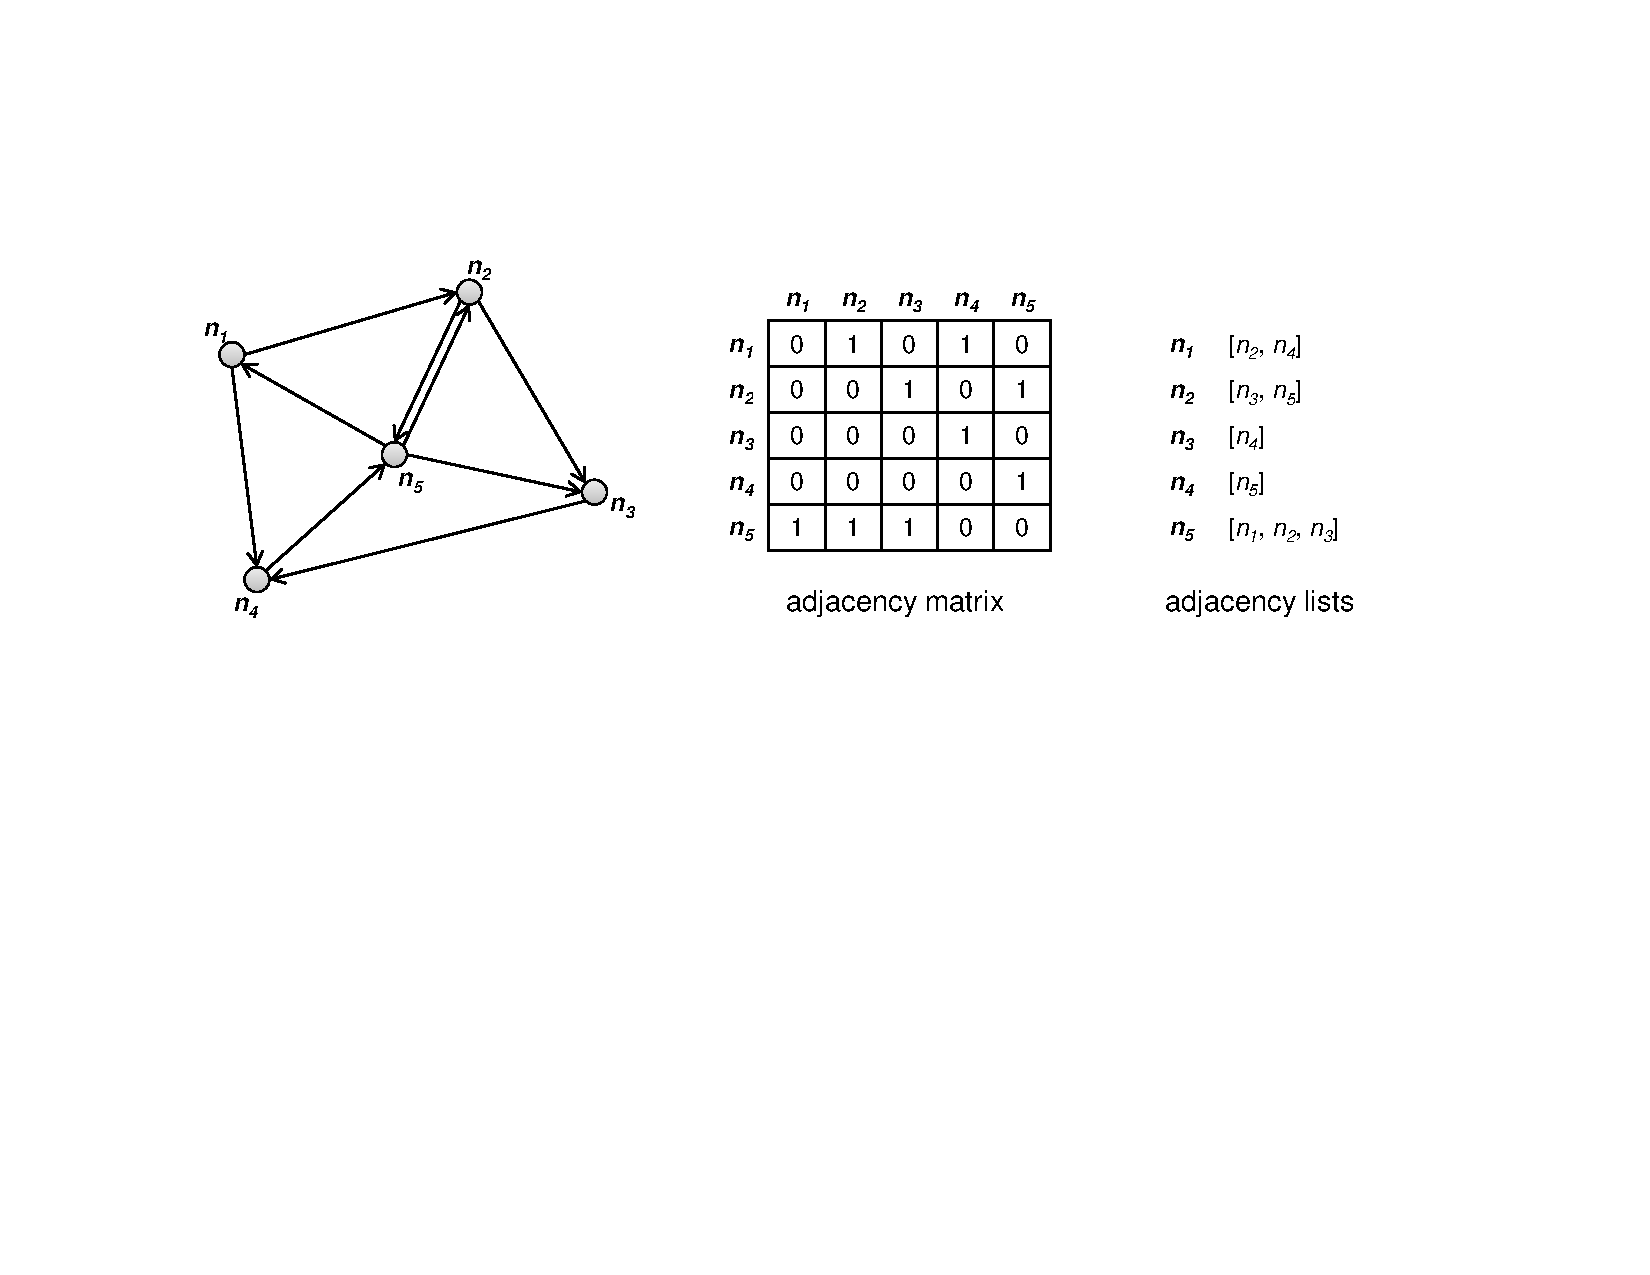
\includegraphics[scale=0.6]{figures/fig-ch5-graph-representations.pdf}
\end{center}
\caption{A simple directed graph (left) represented as an adjacency
  matrix (middle) and with adjacency lists (right).}
\label{figure:chapter-graphs:graph-representations}
\end{figure}

Although mathematicians prefer the adjacency matrix representation of
graphs for easy manipulation with linear algebra, such a
representation is far from ideal for computer scientists concerned
with efficient algorithmic implementations.  Most of the applications
discussed in the chapter introduction involve \emph{sparse} graphs,
where the number of \emph{actual} edges is far smaller than the number
of \emph{possible} edges.\footnote{Unfortunately, there is no precise
  definition of sparseness agreed upon by all, but one common
  definition is that a sparse graph has $O(n)$ edges, where $n$ is the
  number of vertices.}  For example, in a social network of $n$
individuals, there are $n (n-1)$ possible ``friendships'' (where $n$
may be on the order of hundreds of millions).  However, even the most
gregarious will have relatively few friends compared to the size of
the network (thousands, perhaps, but still far smaller than hundreds
of millions).  The same is true for the hyperlink structure of the
web:\ each individual web page links to a minuscule portion of all the
pages on the web.  In this chapter, we assume processing of sparse
graphs, although we will return to this issue in
Section~\ref{chapter-graphs:issues}.

The major problem with an adjacency matrix representation for sparse
graphs is its $O(n^2)$ space requirement.  Furthermore, most of the
cells are zero, by definition.  As a result, most computational
implementations of graph algorithms operate over adjacency lists, in
which a node is associated with neighbors that can be reached via
outgoing edges.
Figure~\ref{figure:chapter-graphs:graph-representations} also shows
the adjacency list representation of the graph under consideration (on
the right).  For example, since $n_1$ is connected by directed edges
to $n_2$ and $n_4$, those two nodes will be on the adjacency list of
$n_1$.  There are two options for encoding undirected graphs:\ one
could simply encode each edge twice (if $n_i$ and $n_j$ are connected,
each appears on each other's adjacency list).  Alternatively, one
could order the nodes (arbitrarily or otherwise) and encode edges only
on the adjacency list of the node that comes first in the ordering
(i.e., if $i<j$, then $n_j$ is on the adjacency list of $n_i$, but not
the other way around).

Note that certain graph operations are easier on adjacency matrices
than on adjacency lists.  In the first, operations on incoming links
for each node translate into a column scan on the matrix, whereas
operations on outgoing links for each node translate into a row scan.
With adjacency lists, it is natural to operate on outgoing links, but
computing anything that requires knowledge of the incoming links of a
node is difficult.  However, as we shall see, the shuffle and sort
mechanism in MapReduce provides an easy way to group edges by their
destination nodes, thus allowing us to compute over incoming edges
with in the reducer.  This property of the execution framework can
also be used to invert the edges of a directed graph, by mapping over
the nodes' adjacency lists and emitting key--value pairs with the
destination node id as the key and the source node id as the
value.\footnote{This technique is used in \emph{anchor text inversion},
  where one gathers the anchor text of hyperlinks pointing to a
  particular page.  It is common practice to enrich a web page's
  standard textual representation with all of the anchor text
  associated with its incoming hyperlinks
  (e.g.,~\cite{Metzler_etal_2009}).}

\section{Parallel Breadth-First Search}
\label{chapter-graphs:BFS}

One of the most common and well-studied problems in graph theory is
the \emph{single-source shortest path} problem, where the task is to
find shortest paths from a source node to all other nodes in the graph
(or alternatively, edges can be associated with costs or weights, in
which case the task is to compute lowest-cost or lowest-weight paths).
Such problems are a staple in undergraduate algorithm courses, where
students are taught the solution using Dijkstra's algorithm.  However,
this famous algorithm assumes sequential processing---how would we
solve this problem in parallel, and more specifically, with MapReduce?

As a refresher and also to serve as a point of comparison, Dijkstra's
algorithm is shown in Figure~\ref{figure:chapter-graphs:Dijkstra},
adapted from Cormen, Leiserson, and Rivest's classic algorithms
textbook~\cite{CLR} (often simply known as \emph{CLR}).  The input to
the algorithm is a directed, connected graph $G=(V,E)$ represented
with adjacency lists, $w$ containing edge distances such that $w(u,v)
\geq 0$, and the source node $s$.  The algorithm begins by first
setting distances to all vertices $d[v], v \in V$ to $\infty$, except
for the source node, whose distance to itself is zero.  The algorithm
maintains $Q$, a global priority queue of vertices with priorities equal to
their distance values $d$.

\begin{figure}[t]
\algrenewcommand\algorithmicfunction{}
  \begin{algorithmic}[1]
    \Function{Dijkstra}{$G, w, s$}
    \State $d[s] \gets 0$
    \ForAll{$\textrm{vertex }v \in V$}
      \State $d[v] \gets \infty$
    \EndFor
    \State $Q \gets \{V\}$
    \While{$Q \ne \emptyset$}
      \State $u \gets \textsc{ExtractMin}(Q)$
      \ForAll{$\textrm{vertex }v \in u.\textsc{AdjacencyList}$}
        \If{$d[v] > d[u] + w(u,v)$}
          \State $d[v] \gets d[u] + w(u,v)$
        \EndIf
      \EndFor
    \EndWhile
    \EndFunction
  \end{algorithmic}
  \caption{Pseudo-code for Dijkstra's algorithm, which is based on
    maintaining a global priority queue of nodes with priorities equal to
    their distances from the source node.  At each iteration, the
    algorithm expands the node with the shortest distance and updates
    distances to all reachable nodes.}
\label{figure:chapter-graphs:Dijkstra}
\end{figure}

Dijkstra's algorithm operates by iteratively selecting the node with
the lowest current distance from the priority queue (initially, this
is the source node).  At each iteration, the algorithm ``expands''
that node by traversing the adjacency list of the selected node to see
if any of those nodes can be reached with a path of a shorter
distance.  The algorithm terminates when the priority queue $Q$ is
empty, or equivalently, when all nodes have been considered.  Note
that the algorithm as presented in
Figure~\ref{figure:chapter-graphs:Dijkstra} only computes the shortest
distances.  The actual paths can be recovered by storing
``backpointers'' for every node indicating a fragment of the shortest
path.

\begin{figure}[t]
\begin{center}
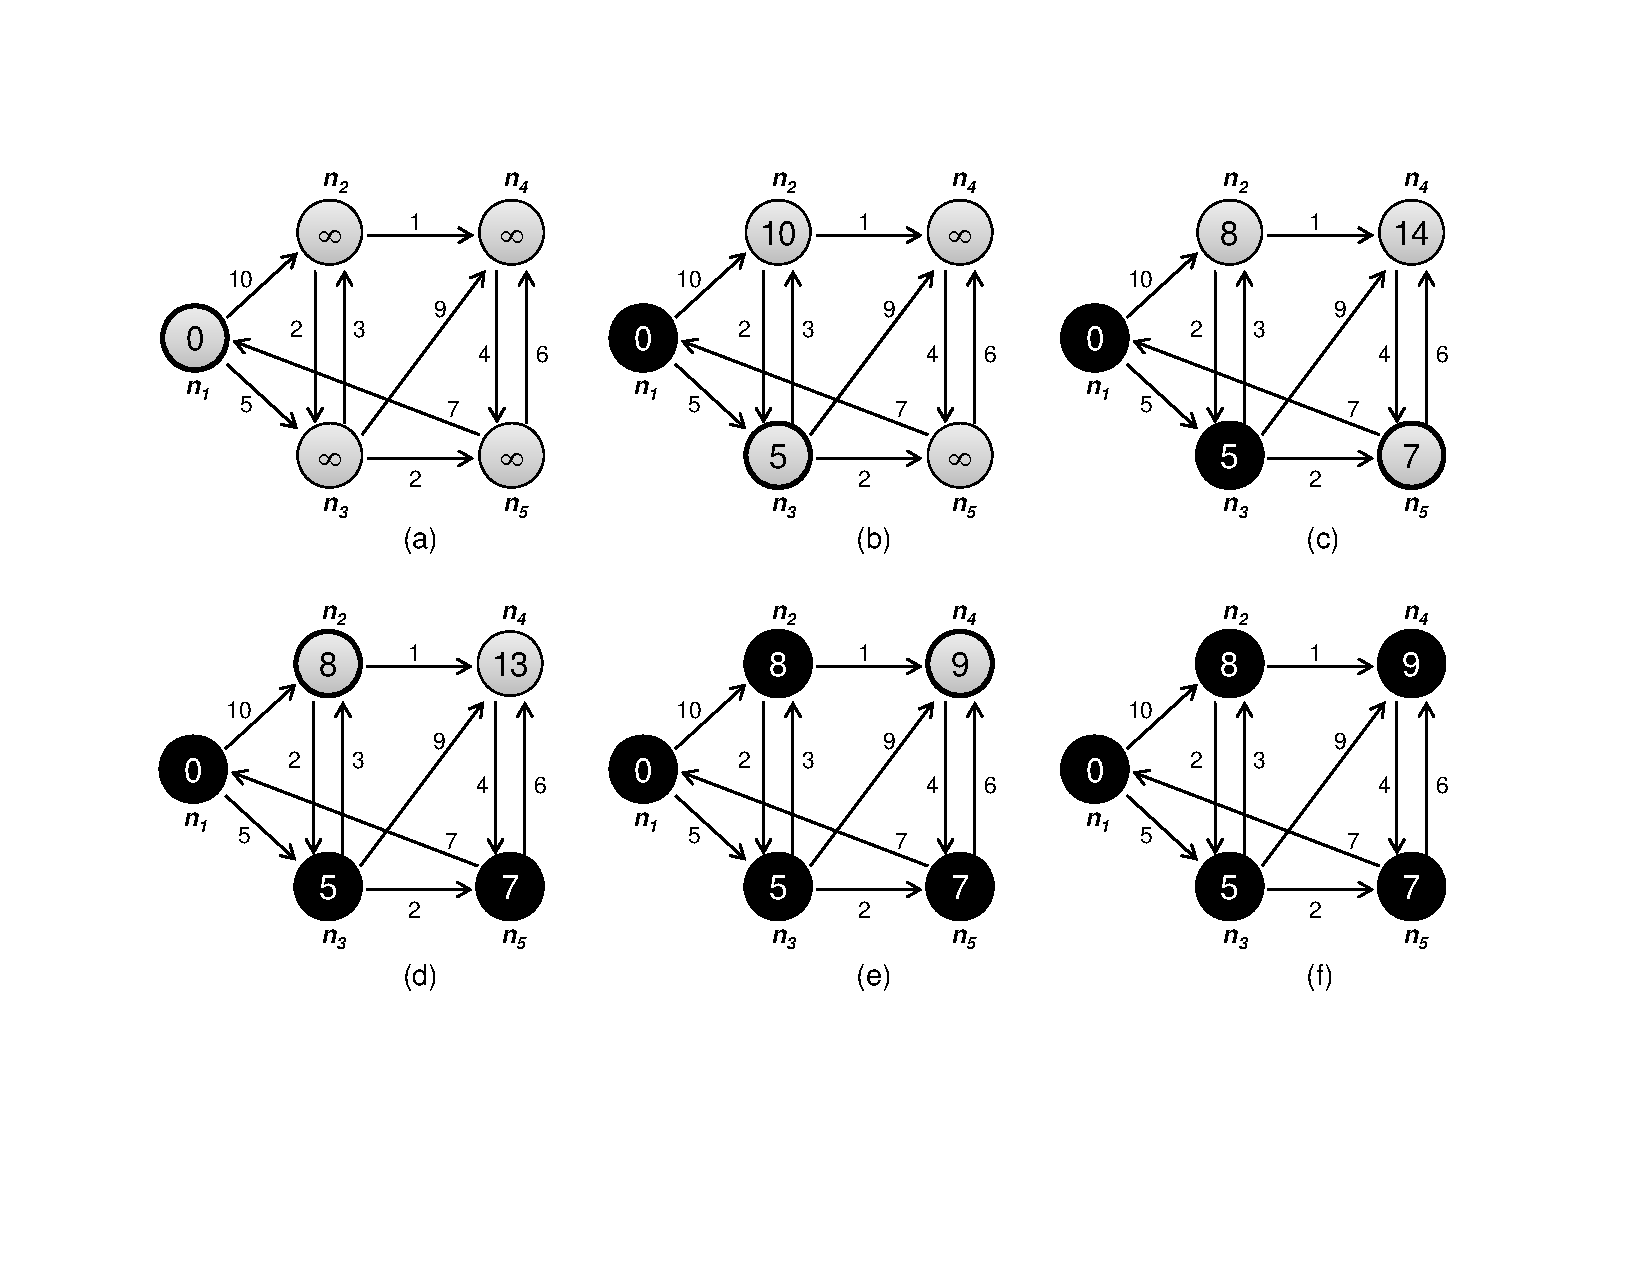
\includegraphics[scale=0.50]{figures/fig-ch5-Dijkstra-example.pdf}
\end{center}
\caption{Example of Dijkstra's algorithm applied to a simple graph
  with five nodes, with $n_1$ as the source and edge distances as
  indicated.  Parts (a)--(e) show the running of the algorithm at each
  iteration, with the current distance inside the node.  Nodes with
  thicker borders are those being expanded; nodes that have already
  been expanded are shown in black.}
\label{figure:chapter-graphs:Dijkstra-example}
\end{figure}

A sample trace of the algorithm running on a simple graph is shown in
Figure~\ref{figure:chapter-graphs:Dijkstra-example} (example also adapted
from \emph{CLR}).  We start out in (a) with $n_1$ having a
distance of zero (since it's the source) and all other nodes having a
distance of $\infty$.  In the first iteration (a), $n_1$ is selected
as the node to expand (indicated by the thicker border).  After the
expansion, we see in (b) that $n_2$ and $n_3$ can be reached at a
distance of 10 and 5, respectively.  Also, we see in (b) that $n_3$ is
the next node selected for expansion.  Nodes we have already
considered for expansion are shown in black.  Expanding $n_3$, we see
in (c) that the distance to $n_2$ has decreased because we've found a
shorter path.  The nodes that will be expanded next, in order, are
$n_5$, $n_2$, and $n_4$.  The algorithm terminates with the end state
shown in (f), where we've discovered the shortest distance to all
nodes.

The key to Dijkstra's algorithm is the priority queue that maintains a
globally-sorted list of nodes by current distance.  This is not
possible in MapReduce, as the programming model does not provide a
mechanism for exchanging global data.  Instead, we adopt a brute force
approach known as parallel breadth-first search.  First, as a
simplification let us assume that all edges have unit distance
(modeling, for example, hyperlinks on the web).  This makes the
algorithm easier to understand, but we'll relax this restriction
later.

The intuition behind the algorithm is this:\ the distance of all nodes
connected directly to the source node is one; the distance of all
nodes directly connected to those is two; and so on.  Imagine water
rippling away from a rock dropped into a pond---that's a good image of
how parallel breadth-first search works.  However, what if there are
multiple paths to the same node?  Suppose we wish to compute the
shortest distance to node $n$.  The shortest path must go through one
of the nodes in $M$ that contains an outgoing edge to $n$:\ we need to
examine all $m \in M$ to find $m_s$, the node with the shortest distance.
The shortest distance to $n$ is the distance to $m_s$ plus one.

Pseudo-code for the implementation of the parallel breadth-first
search algorithm is provided in
Figure~\ref{figure:chapter-graphs:BFS}.  As with Dijkstra's algorithm,
we assume a connected, directed graph represented as adjacency lists.
Distance to each node is directly stored alongside the adjacency list
of that node, and initialized to $\infty$ for all nodes except for the
source node.  In the pseudo-code, we use $n$ to denote the node id (an
integer) and $N$ to denote the node's corresponding data structure
(adjacency list and current distance).  The algorithm works by mapping
over all nodes and emitting a key-value pair for each neighbor on the
node's adjacency list.  The key contains the node id of the neighbor,
and the value is the current distance to the node plus one.  This
says:\ if we can reach node $n$ with a distance $d$, then we must be
able to reach all the nodes that are connected to $n$ with distance
$d+1$.  After shuffle and sort, reducers will receive keys
corresponding to the destination node ids and distances corresponding
to all paths leading to that node.  The reducer will select the
shortest of these distances and then update the distance in the node
data structure.

\begin{figure}[t]
\algrenewcommand\algorithmicfunction{\textbf{class}}
\algrenewcommand\algorithmicprocedure{\textbf{method}}
  \begin{algorithmic}[1]
    \Function{Mapper}{}
    \Procedure{Map}{$\textrm{nid }n, \textrm{node }N$}
    \State $d \gets N.\textsc{Distance}$
    \State $\textsc{Emit}(\textrm{nid }n, N)$\Comment{Pass along graph structure}
    \ForAll{$\textrm{nodeid }m \in N.\textsc{AdjacencyList}$}
      \State $\textsc{Emit}(\textrm{nid }m, d+1)$\Comment{Emit distances to reachable nodes}
    \EndFor
    \EndProcedure
    \EndFunction
  \end{algorithmic}

  \begin{algorithmic}[1]
    \Function{Reducer}{}
    \Procedure{Reduce}{$\textrm{nid }m, [d_1, d_2, \ldots ]$}
    \State $d_{min} \gets \infty$
    \State $M \gets \emptyset$
    \ForAll{$d \in \textrm{counts }[d_1, d_2, \ldots ]$}
      \If{$\textsc{IsNode}(d)$}
        \State $M \gets d$\Comment{Recover graph structure}
      \ElsIf{$d < d_{min}$}\Comment{Look for shorter distance}
        \State $d_{min} \gets d$
      \EndIf
    \EndFor
    \State $M.\textsc{Distance} \gets d_{min}$\Comment{Update shortest distance}
    \State $\textsc{Emit}(\textrm{nid }m, \textrm{node }M)$
    \EndProcedure
    \EndFunction
  \end{algorithmic}
  \caption{Pseudo-code for parallel breath-first search in
    MapReduce:\ the mappers emit distances to reachable nodes, while
    the reducers select the minimum of those distances for each
    destination node.  Each iteration (one MapReduce job) of the
    algorithm expands the ``search frontier'' by one hop.}
\label{figure:chapter-graphs:BFS}
\end{figure}

It is apparent that parallel breadth-first search is an iterative
algorithm, where each iteration corresponds to a MapReduce job.  The
first time we run the algorithm, we ``discover'' all nodes that are
connected to the source.  The second iteration, we discover all nodes
connected to those, and so on.  Each iteration of the algorithm
expands the ``search frontier'' by one hop, and, eventually, all nodes
will be discovered with their shortest distances (assuming a
fully-connected graph).  Before we discuss termination of the
algorithm, there is one more detail required to make the parallel
breadth-first search algorithm work.  We need to ``pass along'' the
graph structure from one iteration to the next.  This is accomplished
by emitting the node data structure itself, with the node id as a key
(Figure~\ref{figure:chapter-graphs:BFS}, line 4 in the mapper).  In the
reducer, we must distinguish the node data structure from distance
values (Figure~\ref{figure:chapter-graphs:BFS}, lines 5--6 in the reducer),
and update the minimum distance in the node data structure before
emitting it as the final value.  The final output is now ready to
serve as input to the next iteration.\footnote{Note that in this
  algorithm we are overloading the value type, which can either be a
  distance (integer) or a complex data structure representing a node.
  The best way to achieve this in Hadoop is to create a wrapper object
  with an indicator variable specifying what the content is.}

So how many iterations are necessary to compute the shortest distance
to all nodes?  The answer is the diameter of the graph, or the
greatest distance between any pair of nodes.  This number is
surprisingly small for many real-world problems:\ the saying ``six
degrees of separation'' suggests that everyone on the planet is
connected to everyone else by at most six steps (the people a person
knows are one step away, people that they know are two steps away,
etc.).  If this is indeed true, then parallel breadth-first search on
the global social network would take at most six MapReduce iterations.
For more serious academic studies of ``small world'' phenomena in
networks, we refer the reader to a number of
publications~\cite{Granovetter73,Granovetter83,Watts_Strogatz_1998,Albert_Barabasi_2002}.
In practical terms, we iterate the algorithm until there are no more
node distances that are $\infty$.  Since the graph is connected, all
nodes are reachable, and since all edge distances are one, all
discovered nodes are guaranteed to have the shortest distances (i.e.,
there is not a shorter path that goes through a node that hasn't been
discovered).

The actual checking of the termination condition must occur outside of
MapReduce.  Typically, execution of an iterative MapReduce algorithm
requires a non-MapReduce ``driver'' program, which submits a MapReduce
job to iterate the algorithm, checks to see if a termination condition
has been met, and if not, repeats.  Hadoop provides a lightweight API
for constructs called ``counters'', which, as the name suggests, can be
used for counting events that occur during execution, e.g., number
of corrupt records, number of times a certain condition is met, or
anything that the programmer desires.  Counters can be defined to
count the number of nodes that have distances of $\infty$:\ at the end
of the job, the driver program can access the final counter value and
check to see if another iteration is necessary.

Finally, as with Dijkstra's algorithm in the form presented earlier,
the parallel breadth-first search algorithm only finds the shortest
distances, not the actual shortest paths.  However, the path can be
straightforwardly recovered.  Storing ``backpointers'' at each node,
as with Dijkstra's algorithm, will work, but may not be efficient
since the graph needs to be traversed again to reconstruct the path
segments.  A simpler approach is to emit paths along with distances in
the mapper, so that each node will have its shortest path easily
accessible at all times.  The additional space requirements for
shuffling these data from mappers to reducers are relatively modest,
since for the most part paths (i.e., sequence of node ids) are relatively short.

\begin{figure}[t]
\begin{center}
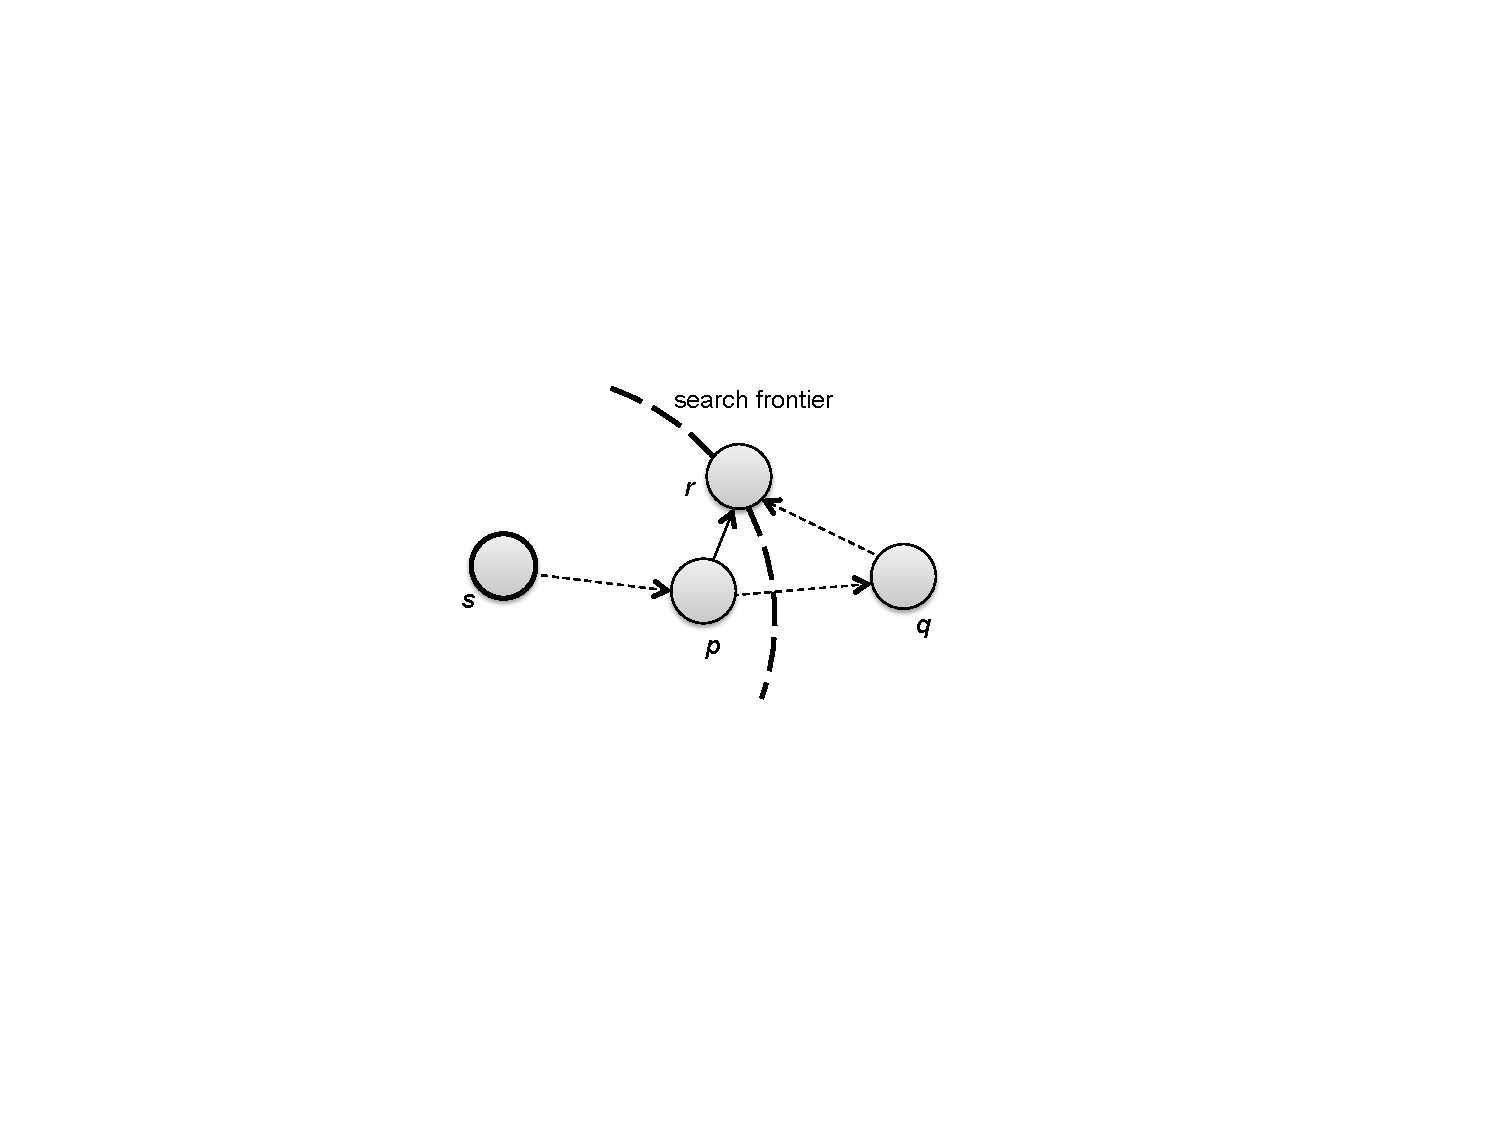
\includegraphics[scale=0.6]{figures/fig-ch5-search-frontier.pdf}
\end{center}
\caption{In the single source shortest path problem with arbitrary
  edge distances, the shortest path from source $s$ to node $r$ may go
  outside the current search frontier, in which case we will not find
  the shortest distance to $r$ until the search frontier expands to
  cover $q$.}
\label{figure:chapter-graphs:search-frontier}
\end{figure}

Up until now, we have been assuming that all edges are unit distance.
Let us relax that restriction and see what changes are required in the
parallel breadth-first search algorithm.  The adjacency lists, which
were previously lists of node ids, must now encode the edge distances
as well.  In line 6 of the mapper code in
Figure~\ref{figure:chapter-graphs:BFS}, instead of emitting $d+1$ as
the value, we must now emit $d+w$ where $w$ is the edge distance.  No
other changes to the algorithm are required, but the termination
behavior is very different.  To illustrate, consider the graph
fragment in Figure~\ref{figure:chapter-graphs:search-frontier}, where
$s$ is the source node, and in this iteration, we just ``discovered''
node $r$ for the very first time.  Assume for the sake of argument
that we've already discovered the shortest distance to node $p$, and
that the shortest distance to $r$ so far goes through $p$.  This,
however, does not guarantee that we've discovered the shortest
distance to $r$, since there may exist a path going through $q$ that
we haven't encountered yet (because it lies outside the search
frontier).\footnote{Note that the same argument does not apply to the
  unit edge distance case:\ the shortest path cannot lie outside the
  search frontier since any such path would necessarily be longer.}
However, as the search frontier expands, we'll eventually cover $q$
and all other nodes along the path from $p$ to $q$ to $r$---which
means that with sufficient iterations, we will discover the shortest
distance to $r$.  But how do we know that we've found the shortest
distance to $p$?  Well, if the shortest path to $p$ lies within the
search frontier, we would have already discovered it.  And if it
doesn't, the above argument applies.  Similarly, we can repeat the
same argument for all nodes on the path from $s$ to $p$.  The
conclusion is that, with sufficient iterations, we'll eventually
discover all the shortest distances.

\begin{figure}[t]
\begin{center}
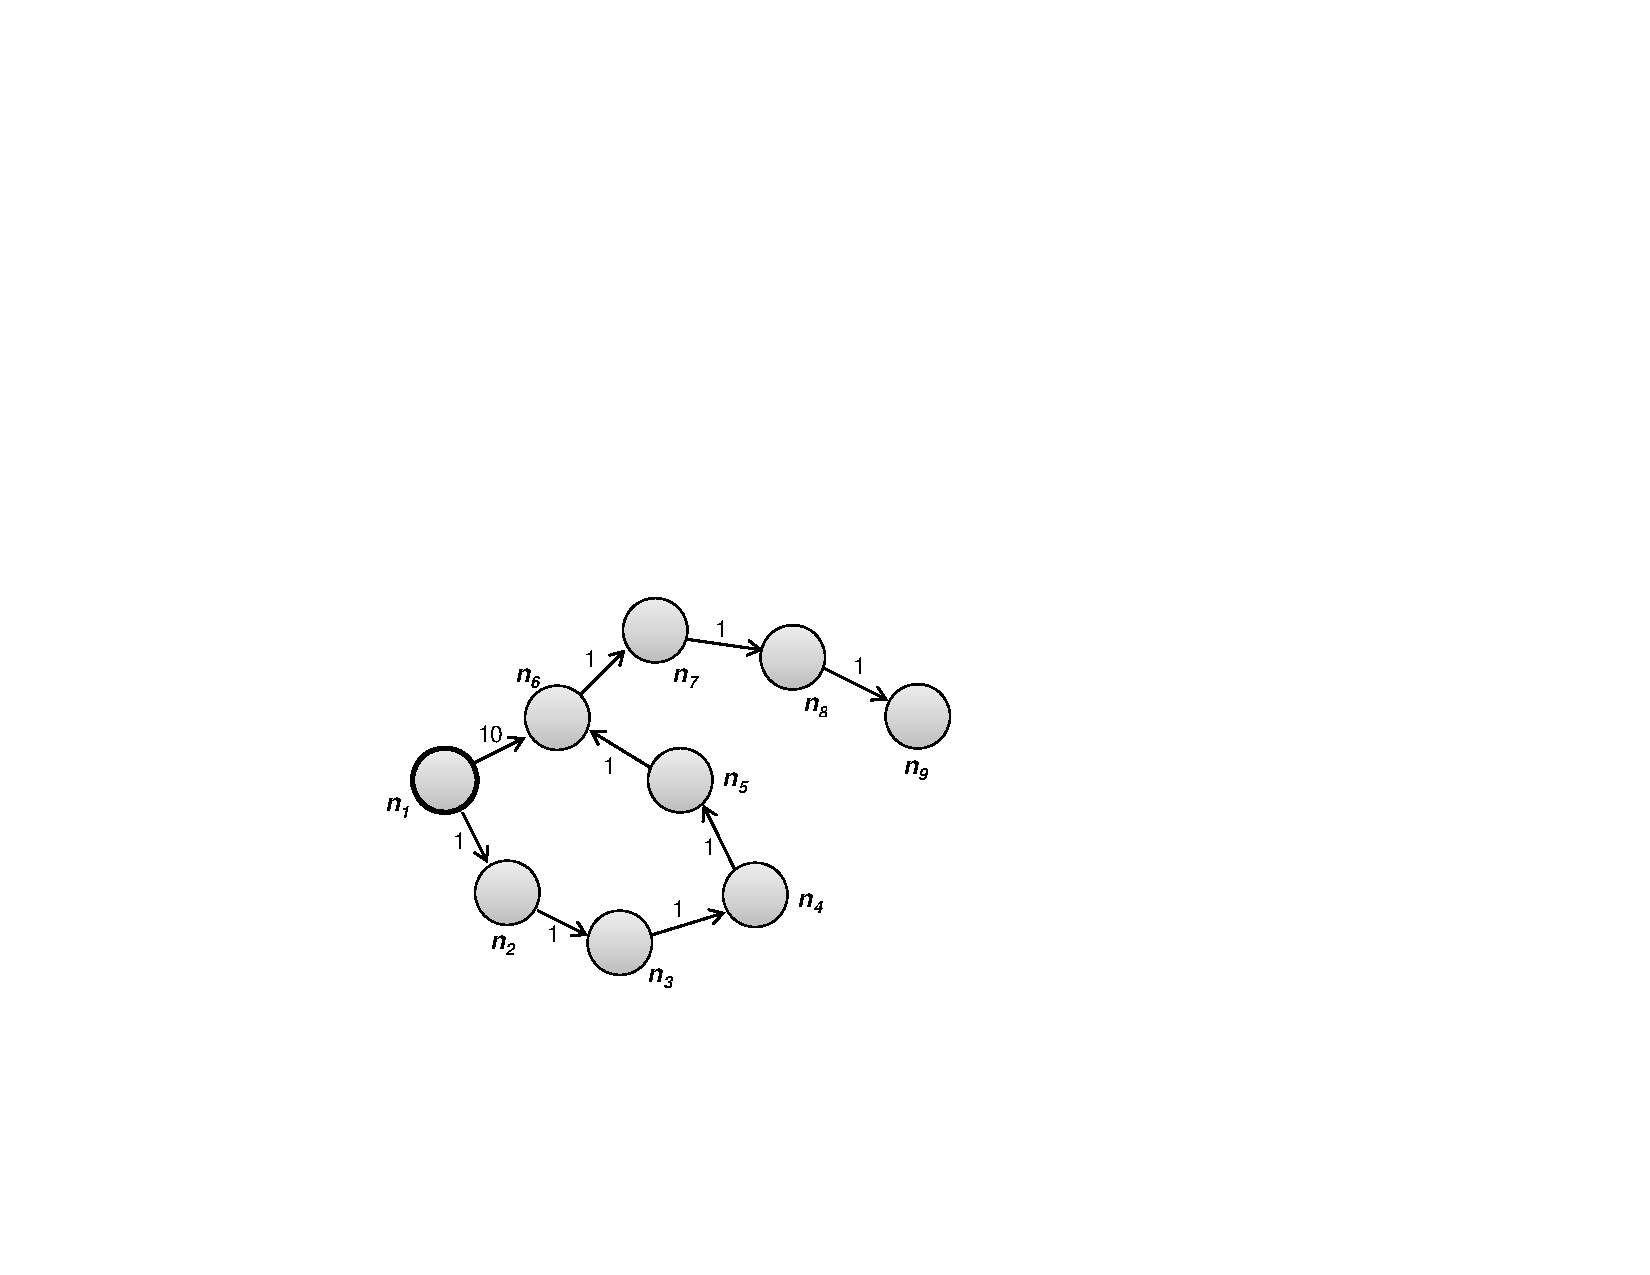
\includegraphics[scale=0.6]{figures/fig-ch5-screwy-graph.pdf}
\end{center}
\caption{A sample graph that elicits worst-case behavior for parallel
  breadth-first search.  Eight iterations are required to discover
  shortest distances to all nodes from $n_1$.}
\label{figure:chapter-graphs:screwy-graph}
\end{figure}

So exactly how many iterations does ``eventually'' mean?  In the worst
case, we might need as many iterations as there are nodes in the graph
minus one.  In fact, it is not difficult to construct graphs that will
elicit this worse-case
behavior:\ Figure~\ref{figure:chapter-graphs:screwy-graph} provides an
example, with $n_1$ as the source.  The parallel breadth-first search
algorithm would not discover that the shortest path from $n_1$ to
$n_6$ goes through $n_3$, $n_4$, and $n_5$ until the fifth iteration.
Three more iterations are necessary to cover the rest of the graph.
Fortunately, for most real-world graphs, such extreme cases are rare,
and the number of iterations necessary to discover all shortest
distances is quite close to the diameter of the graph, as in the unit
edge distance case.

In practical terms, how do we know when to stop iterating in the case
of arbitrary edge distances?  The algorithm can terminate when
shortest distances at every node no longer change.  Once again, we can
use counters to keep track of such events.  Every time we encounter a
shorter distance in the reducer, we increment a counter.  At the end
of each MapReduce iteration, the driver program reads the counter
value and determines if another iteration is necessary.

Compared to Dijkstra's algorithm on a single processor, parallel
breadth-first search in MapReduce can be characterized as a brute
force approach that ``wastes'' a lot of time performing computations
whose results are discarded.  At each iteration, the algorithm
attempts to recompute distances to all nodes, but in reality only
useful work is done along the search frontier:\ inside the search
frontier, the algorithm is simply repeating previous
computations.\footnote{Unless the algorithm discovers an instance of
  the situation described in
  Figure~\ref{figure:chapter-graphs:search-frontier}, in which case,
  updated distances will propagate inside the search frontier.}
Outside the search frontier, the algorithm hasn't discovered any paths
to nodes there yet, so no meaningful work is done.  Dijkstra's
algorithm, on the other hand, is far more efficient.  Every time a
node is explored, we're guaranteed to have already found the shortest
path to it.  However, this is made possible by maintaining a global
data structure (a priority queue) that holds nodes sorted by
distance---this is not possible in MapReduce because the programming
model does not provide support for global data that is mutable and
accessible by the mappers and reducers.  These inefficiencies
represent the cost of parallelization.

The parallel breadth-first search algorithm is instructive in that it
represents the prototypical structure of a large class of graph
algorithms in MapReduce.  They share in the following characteristics:

\begin{itemize}

\item The graph structure is represented with adjacency lists, which is
  part of some larger node data structure that may contain additional
  information (variables to store intermediate output, features of the
  nodes).  In many cases, features are attached to edges as well
  (e.g., edge weights).

\item The MapReduce algorithm maps over the node data structures and
  performs a computation that is a function of features of the node,
  intermediate output attached to each node, and features of the
  adjacency list (outgoing edges and their features).  In other words,
  computations can only involve a node's internal state and its local
  graph structure.  The results of these computations are emitted as
  values, keyed with the node ids of the neighbors (i.e., those nodes
  on the adjacency lists).  Conceptually, we can think of this as
  ``passing'' the results of the computation along outgoing edges.  In
  the reducer, the algorithm receives all partial results that have
  the same destination node, and performs another computation
  (usually, some form of aggregation).

\item In addition to computations, the graph itself is also passed
  from the mapper to the reducer.  In the reducer, the data structure
  corresponding to each node is updated and written back to disk.

\item Graph algorithms in MapReduce are generally iterative, where the
  output of the previous iteration serves as input to the next
  iteration.  The process is controlled by a non-MapReduce driver
  program that checks for termination.

\end{itemize}

\noindent For parallel breadth-first search, the mapper computation is
the current distance plus edge distance (emitting distances to
neighbors), while the reducer computation is the \textsc{Min} function
(selecting the shortest path).  As we will see in the next section,
the MapReduce algorithm for PageRank works in much the same way.

\section{PageRank}
\label{chapter-graphs:PageRank}

PageRank~\cite{Page_etal_1999} is a measure of web page quality based
on the structure of the hyperlink graph.  Although it is only one of
thousands of features that is taken into account in Google's search
algorithm, it is perhaps one of the best known and most studied.

A vivid way to illustrate PageRank is to imagine a random web
surfer:\ the surfer visits a page, randomly clicks a link on that
page, and repeats ad infinitum.  PageRank is a measure of how
frequently a page would be encountered by our tireless web surfer.
More precisely, PageRank is a probability distribution over nodes in
the graph representing the likelihood that a random walk over the link
structure will arrive at a particular node.  Nodes that have high
in-degrees tend to have high PageRank values, as well as nodes that
are linked to by other nodes with high PageRank values.  This behavior
makes intuitive sense:\ if PageRank is a measure of page quality, we
would expect high-quality pages to contain ``endorsements'' from many
other pages in the form of hyperlinks.  Similarly, if a high-quality
page links to another page, then the second page is likely to be high
quality also.  PageRank represents one particular approach to
inferring the quality of a web page based on hyperlink structure; two
other popular algorithms, not covered here, are
SALSA~\cite{Lempel_Moran_TOIS2001} and HITS~\cite{Kleinberg_JACM1999}
(also known as ``hubs and authorities'').

The complete formulation of PageRank includes an additional component.
As it turns out, our web surfer doesn't just randomly click links.
Before the surfer decides where to go next, a biased coin is
flipped---heads, the surfer clicks on a random link on the page as
usual.  Tails, however, the surfer ignores the links on the page and
randomly ``jumps'' or ``teleports'' to a completely different page.

But enough about random web surfing.  Formally, the PageRank $P$ of a
page $n$ is defined as follows:

\begin{equation}
P(n) = \alpha \left( \frac{1}{|G|} \right) + (1-\alpha) \sum_{m \in L(n)} \frac{P(m)}{C(m)}
\end{equation}

\noindent where $|G|$ is the total number of nodes (pages) in the
graph, $\alpha$ is the random jump factor, $L(n)$ is the set of pages
that link to $n$, and $C(m)$ is the out-degree of node $m$ (the number
of links on page $m$).  The random jump factor $\alpha$ is sometimes
called the ``teleportation'' factor; alternatively, $(1-\alpha)$ is
referred to as the ``damping'' factor.

Let us break down each component of the formula in detail.  First,
note that PageRank is defined recursively---this gives rise to an
iterative algorithm we will detail in a bit.  A web page $n$ receives
PageRank ``contributions'' from all pages that link to it, $L(n)$.
Let us consider a page $m$ from the set of pages $L(n)$:\ a random
surfer at $m$ will arrive at $n$ with probability $1/C(m)$ since a
link is selected at random from all outgoing links.  Since the PageRank
value of $m$ is the probability that the random surfer will be at $m$,
the probability of arriving at $n$ from $m$ is $P(m)/C(m)$.  To
compute the PageRank of $n$, we need to sum contributions from all
pages that link to $n$.  This is the summation in the second half of
the equation.  However, we also need to take into account the random
jump:\ there is a $1/|G|$ chance of landing at any particular page,
where $|G|$ is the number of nodes in the graph.  Of course, the two
contributions need to be combined:\ with probability $\alpha$ the
random surfer executes a random jump, and with probability $1-\alpha$
the random surfer follows a hyperlink.

Note that PageRank assumes a community of honest users who are not
trying to ``game'' the measure.  This is, of course, not true in the
real world, where an adversarial relationship exists between search
engine companies and a host of other organizations and individuals
(marketers, spammers, activists, etc.) who are trying to manipulate
search results---to promote a cause, product, or service, or in some
cases, to trap and intentionally deceive users (see, for
example,~\cite{Baeza-Yates_etal_2005,Garcia-Molina_etal_2005}).  A
simple example is a so-called ``spider trap'', a infinite chain of
pages (e.g., generated by CGI) that all link to a single page (thereby
artificially inflating its PageRank).  For this reason, PageRank is
only one of thousands of features used in ranking web pages.

The fact that PageRank is recursively defined 
translates into an iterative algorithm which is quite similar in basic
structure to parallel breadth-first search.  We start by presenting an
informal sketch.  At the beginning of each iteration, a node passes its
PageRank contributions to other nodes that it is connected to.  Since
PageRank is a probability distribution, we can think of this as
spreading probability mass to neighbors via outgoing links.  To
conclude the iteration, each node sums up all PageRank contributions
that have been passed to it and computes an updated PageRank score.
We can think of this as gathering probability mass passed to a node
via its incoming links.  This algorithm iterates until PageRank values
don't change anymore.

\begin{figure}[t]
\begin{center}
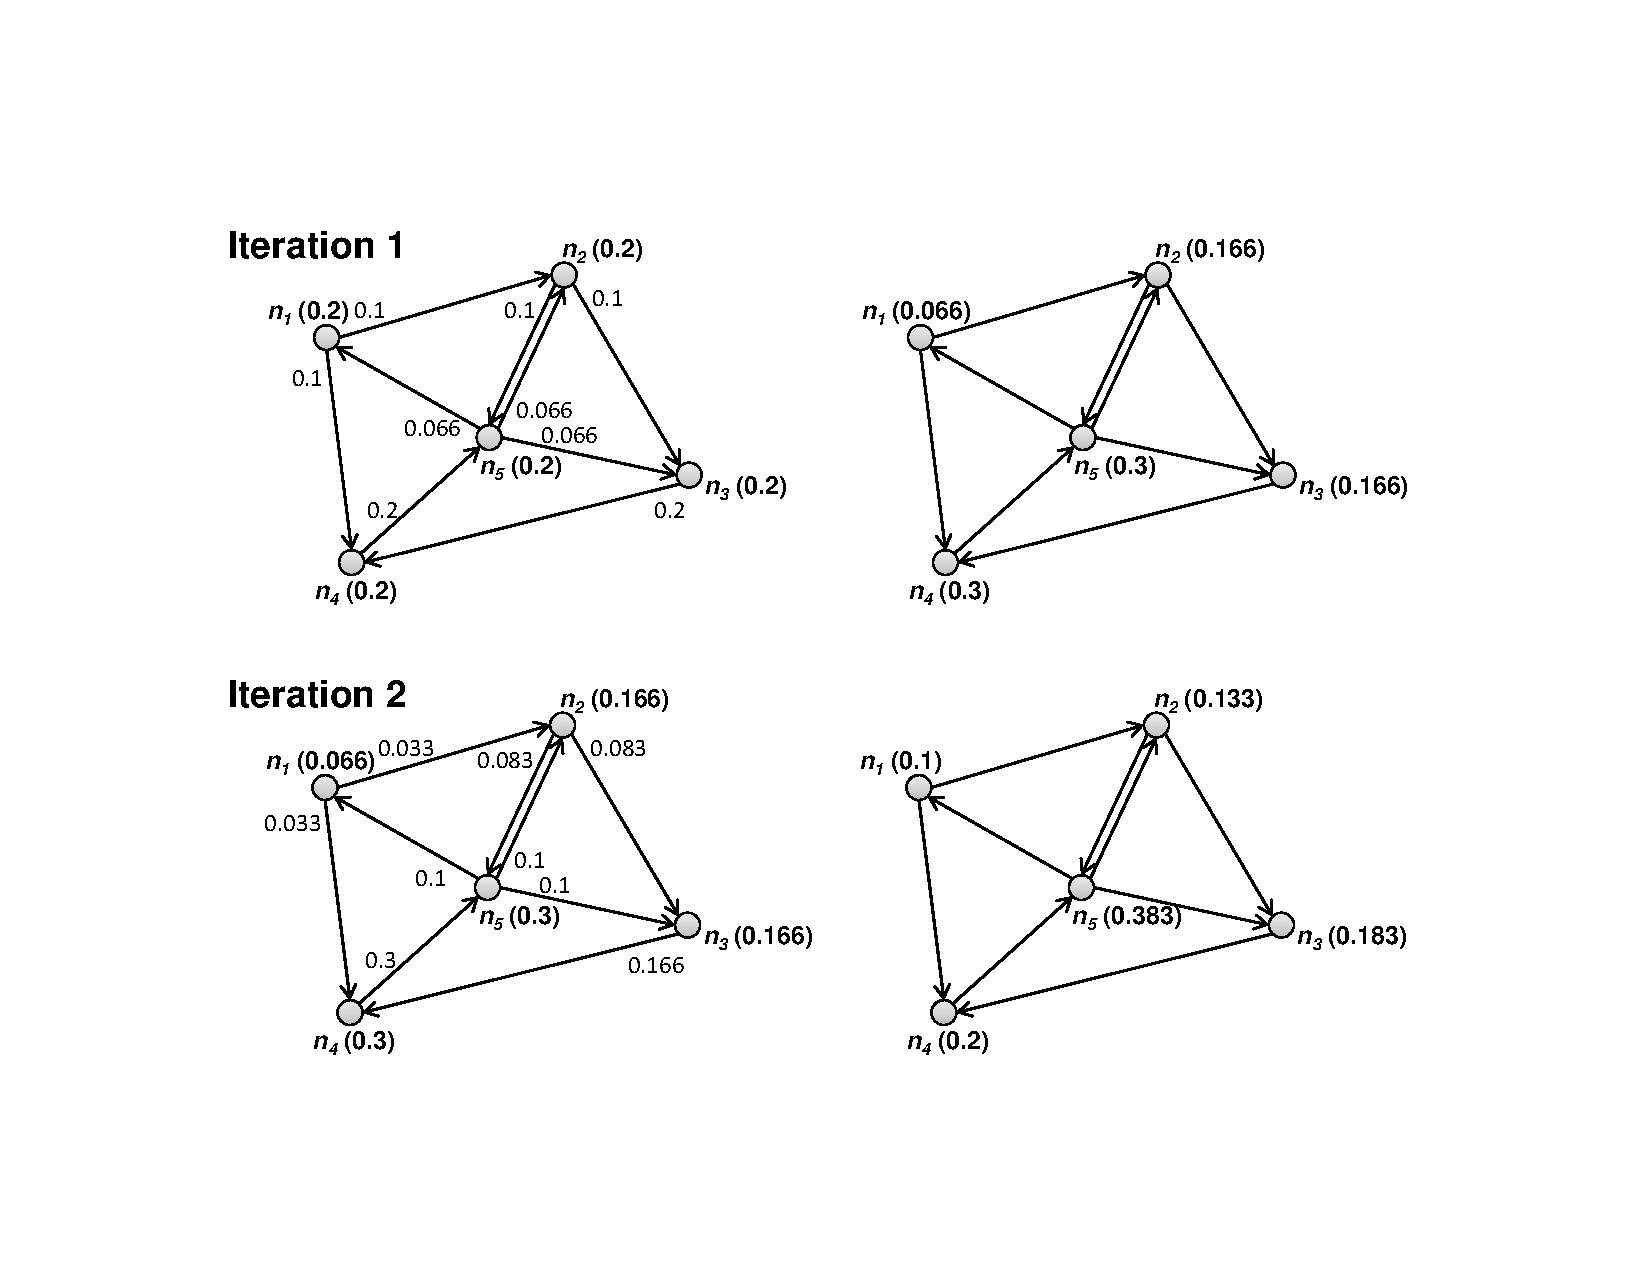
\includegraphics[scale=0.6]{figures/fig-ch5-PageRank-toy-example.pdf}
\end{center}
\caption{PageRank toy example showing two iterations, top and bottom.
  Left graphs show PageRank values at the beginning of each iteration
  and how much PageRank mass is passed to each neighbor.  Right graphs
  show updated PageRank values at the end of each iteration.}
\label{figure:chapter-graphs:PageRank-toy}
\end{figure}

Figure~\ref{figure:chapter-graphs:PageRank-toy} shows a toy example that
illustrates two iterations of the algorithm.  As a simplification, we
ignore the random jump factor for now (i.e., $\alpha=0$) and further
assume that there are no dangling nodes (i.e., nodes with no outgoing
edges).  The algorithm begins by initializing a uniform distribution
of PageRank values across nodes.  In the beginning of the first
iteration (top, left), partial PageRank contributions are sent from
each node to its neighbors connected via outgoing links.  For example,
$n_1$ sends $0.1$ PageRank mass to $n_2$ and $0.1$ PageRank mass to
$n_4$.  This makes sense in terms of the random surfer model:\ if the
surfer is at $n_1$ with a probability of $0.2$, then the surfer could end up
either in $n_2$ or $n_4$ with a probability of $0.1$ each.  The same
occurs for all the other nodes in the graph:\ note that $n_5$ must
split its PageRank mass three ways, since it has three neighbors, and
$n_4$ receives all the mass belonging to $n_3$ because $n_3$ isn't
connected to any other node.  The end of the first iteration is shown
in the top right:\ each node sums up PageRank contributions from its
neighbors.  Note that since $n_1$ has only one incoming link, from
$n_3$, its updated PageRank value is smaller than before, i.e., it
``passed along'' more PageRank mass than it received.  The exact same
process repeats, and the second iteration in our toy example is
illustrated by the bottom two graphs.  At the beginning of each
iteration, the PageRank values of all nodes sum to one.  PageRank mass
is preserved by the algorithm, guaranteeing that we continue to have a
valid probability distribution at the end of each iteration.

Pseudo-code of the MapReduce PageRank algorithm is shown in
Figure~\ref{figure:chapter-graphs:PageRank}; it is simplified in that we
continue to ignore the random jump factor and assume no dangling nodes
(complications that we will return to later).  An illustration of the
running algorithm is shown in
Figure~\ref{figure:chapter-graphs:PageRank-MapReduce-example} for the first
iteration of the toy graph in
Figure~\ref{figure:chapter-graphs:PageRank-toy}.  The algorithm maps over
the nodes, and for each node computes how much PageRank mass needs to
be distributed to its neighbors (i.e., nodes on the adjacency list).
Each piece of the PageRank mass is emitted as the value, keyed by the node
ids of the neighbors.  Conceptually, we can think of this as passing
PageRank mass along outgoing edges.

\begin{figure}[t]
\algrenewcommand\algorithmicfunction{\textbf{class}}
\algrenewcommand\algorithmicprocedure{\textbf{method}}
  \begin{algorithmic}[1]
    \Function{Mapper}{}
    \Procedure{Map}{$\textrm{nid }n, \textrm{node }N$}
    \State $p \gets N.\textsc{PageRank} / |N.\textsc{AdjacencyList}|$
    \State $\textsc{Emit}(\textrm{nid }n, N)$\Comment{Pass along graph structure}
    \ForAll{$\textrm{nodeid }m \in N.\textsc{AdjacencyList}$}
      \State $\textsc{Emit}(\textrm{nid }m, p)$\Comment{Pass PageRank mass to neighbors}
    \EndFor
    \EndProcedure
    \EndFunction
  \end{algorithmic}

  \begin{algorithmic}[1]
    \Function{Reducer}{}
    \Procedure{Reduce}{$\textrm{nid }m, [p_1, p_2, \ldots ]$}
    \State $M \gets \emptyset$
    \ForAll{$p \in \textrm{counts }[p_1, p_2, \ldots ]$}
      \If{$\textsc{IsNode}(p)$}
        \State $M \gets p$\Comment{Recover graph structure}
      \Else
        \State $s \gets s + p$\Comment{Sum incoming PageRank contributions}
      \EndIf
    \EndFor
    \State $M.\textsc{PageRank} \gets s$
    \State $\textsc{Emit}(\textrm{nid }m, \textrm{node }M)$
    \EndProcedure
    \EndFunction
  \end{algorithmic}
  \caption{Pseudo-code for PageRank in MapReduce (leaving aside
    dangling nodes and the random jump factor).  In the map phase we
    evenly divide up each node's PageRank mass and pass each piece
    along outgoing edges to neighbors.  In the reduce phase PageRank
    contributions are summed up at each destination node.  Each
    MapReduce job corresponds to one iteration of the algorithm.}
\label{figure:chapter-graphs:PageRank}
\end{figure}

\begin{figure}[t]
\begin{center}
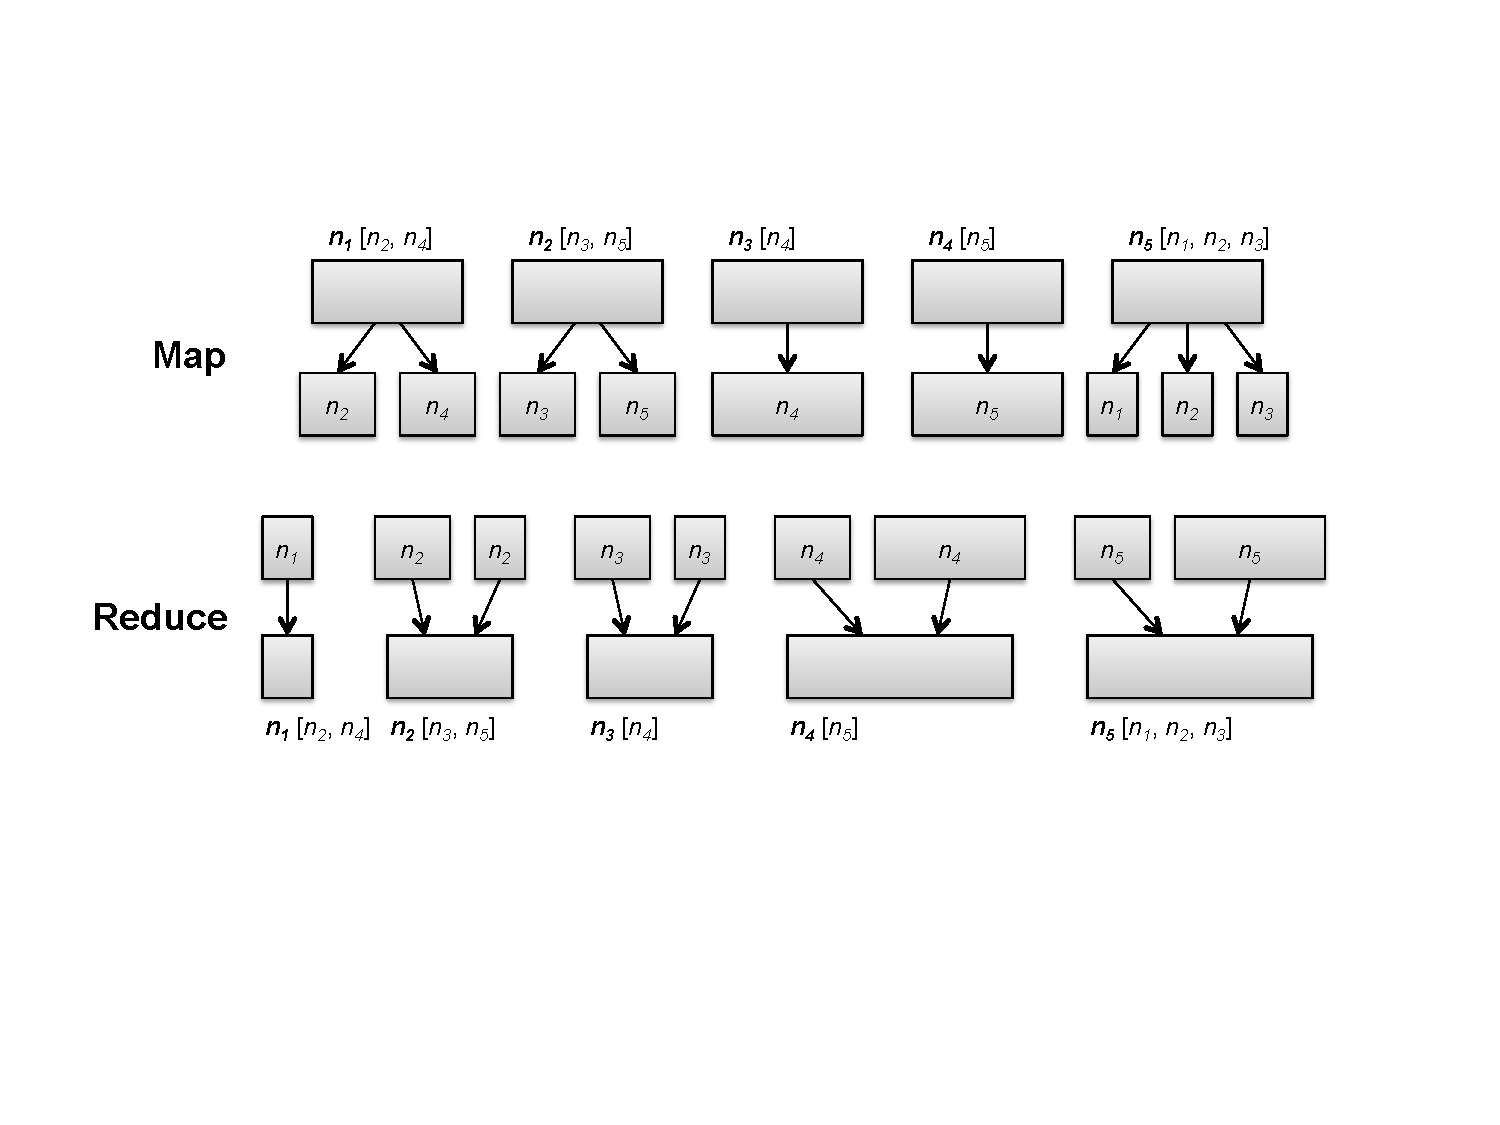
\includegraphics[scale=0.55]{figures/fig-ch5-MapReduce-example.pdf}
\end{center}
\caption{Illustration of the MapReduce PageRank algorithm
  corresponding to the first iteration in
  Figure~\ref{figure:chapter-graphs:PageRank-toy}.  The size of each
  box is proportion to its PageRank value.  During the map phase,
  PageRank mass is distributed evenly to nodes on each node's
  adjacency list (shown at the very top).  Intermediate values are
  keyed by node (shown inside the boxes).  In the reduce phase, all
  partial PageRank contributions are summed together to arrive at
  updated values.}
\label{figure:chapter-graphs:PageRank-MapReduce-example}
\end{figure}

In the shuffle and sort phase, the MapReduce execution framework
groups values (piece of PageRank mass) passed along the graph edges by
destination node (i.e., all edges that point to the same node).  In
the reducer, PageRank mass contributions from all incoming edges are
summed to arrive at the updated PageRank value for each node.  As with
the parallel breadth-first search algorithm, the graph structure
itself must be passed from iteration to iteration.  Each node data
structure is emitted in the mapper and written back out to disk in the
reducer.  All PageRank mass emitted by the mappers are accounted for
in the reducer:\ since we begin with the sum of PageRank values across
all nodes equal to one, the sum of all the updated PageRank values
should remain a valid probability distribution.

Having discussed the simplified PageRank algorithm in MapReduce, let
us now take into account the random jump factor and dangling
nodes:\ as it turns out both are treated similarly.  Dangling nodes
are nodes in the graph that have no outgoing edges, i.e., their
adjacency lists are empty.  In the hyperlink graph of the web, these
might correspond to pages in a crawl that have not been downloaded
yet.  If we simply run the algorithm in
Figure~\ref{figure:chapter-graphs:PageRank} on graphs with dangling nodes,
the total PageRank mass will not be conserved, since no key-value
pairs will be emitted when a dangling node is encountered in the
mappers.

The proper treatment of PageRank mass ``lost'' at the dangling nodes
is to redistribute it across all nodes in the graph evenly
(cf.~\cite{Bianchini_etal_2005}).  There are many ways to determine
the missing PageRank mass.  One simple approach is by instrumenting
the algorithm in Figure~\ref{figure:chapter-graphs:PageRank} with
counters:\ whenever the mapper processes a node with an empty
adjacency list, it keeps track of the node's PageRank value in the
counter.  At the end of the iteration, we can access the counter to
find out how much PageRank mass was lost at the dangling
nodes.\footnote{In Hadoop, counters are 8-byte integers:\ a simple
  workaround is to multiply PageRank values by a large constant, and
  then cast as an integer.}  Another approach is to reserve a special
key for storing PageRank mass from dangling nodes.  When the mapper
encounters a dangling node, its PageRank mass is emitted with the
special key; the reducer must be modified to contain special logic for
handling the missing PageRank mass.  Yet another approach is to write
out the missing PageRank mass as ``side data'' for each map task
(using the in-mapper combining technique for aggregation); a final
pass in the driver program is needed to sum the mass across all map
tasks.  Either way, we arrive at the amount of PageRank mass lost at
the dangling nodes---this then must be redistribute evenly across all
nodes.

This redistribution process can be accomplished by mapping over all
nodes again.  At the same time, we can take into account the random
jump factor.  For each node, its current PageRank value $p$ is updated
to the final PageRank value $p'$ according to the following formula:

\begin{equation}
p' = \alpha \left( \frac{1}{|G|} \right) + \left( 1-\alpha \right) \left( \frac{m}{|G|} + p \right)
\end{equation}

\noindent where $m$ is the missing PageRank mass, and $|G|$ is the
number of nodes in the entire graph.  We add the PageRank mass from
link traversal ($p$, computed from before) to the share of the lost
PageRank mass that is distributed to each node ($m/|G|$).  Finally, we
take into account the random jump factor:\ with probability $\alpha$
the random surfer arrives via jumping, and with probability $1-\alpha$
the random surfer arrives via incoming links.  Note that this
MapReduce job requires no reducers.

Putting everything together, one iteration of PageRank requires two
MapReduce jobs:\ the first to distribute PageRank mass along graph
edges, and the second to take care of dangling nodes and the random
jump factor.  At end of each iteration, we end up with
exactly the same data structure as the beginning, which is a
requirement for the iterative algorithm to work.  Also, the PageRank
values of all nodes sum up to one, which ensures a valid probability
distribution.

Typically, PageRank is iterated until convergence, i.e., when the
PageRank values of nodes no longer change (within some tolerance, to
take into account, for example, floating point precision errors).
Therefore, at the end of each iteration, the PageRank driver program
must check to see if convergence has been reached.  Alternative
stopping criteria include running a fixed number of iterations (useful
if one wishes to bound algorithm running time) or stopping when the
\emph{ranks} of PageRank values no longer change.  The latter is useful
for some applications that only care about comparing the PageRank of
two arbitrary pages and do not need the actual PageRank values.  Rank
stability is obtained faster than the actual convergence of values.

In absolute terms, how many iterations are necessary for PageRank to
converge?  This is a difficult question to \emph{precisely} answer
since it depends on many factors, but generally, fewer than one might
expect.  In the original PageRank paper~\cite{Page_etal_1999},
convergence on a graph with 322 million edges was reached in 52
iterations (see also Bianchini et al.~\cite{Bianchini_etal_2005} for
additional discussion).  On today's web, the answer is not very
meaningful due to the adversarial nature of web search as previously
discussed---the web is full of spam and populated with sites that are
actively trying to ``game'' PageRank and related hyperlink-based
metrics.  As a result, running PageRank in its unmodified form
presented here would yield unexpected and undesirable results.  Of
course, strategies developed by web search companies to combat link
spam are proprietary (and closely-guarded secrets, for obvious
reasons)---but undoubtedly these algorithmic modifications impact
convergence behavior.  A full discussion of the escalating ``arms
race'' between search engine companies and those that seek to promote
their sites is beyond the scope of this book.\footnote{For the
  interested reader, the proceedings of a workshop series on
  Adversarial Information Retrieval (AIRWeb) provide great starting
  points into the literature.}

\section{Issues with Graph Processing}
\label{chapter-graphs:issues}

The biggest difference between MapReduce graph algorithms and
single-machine graph algorithms is that with the latter, it is usually
possible to maintain global data structures in memory for fast, random
access.  For example, Dijkstra's algorithm uses a global priority
queue that guides the expansion of nodes.  This, of course, is not
possible with MapReduce---the programming model does not provide any
built-in mechanism for communicating global state.  Since the most
natural representation of large sparse graphs is with adjacency lists,
communication can only occur from a node to the nodes it links to, or
to a node from nodes linked to it---in other words, passing
information is only possible within the local graph
structure.\footnote{Of course, it is perfectly reasonable to compute
  derived graph structures in a pre-processing step.  For example, if
  one wishes to propagate information from a node to all nodes that
  are within two links, one could process graph $G$ to derive graph
  $G'$, where there would exist a link from node $n_i$ to $n_j$ if
  $n_j$ was reachable within two link traversals of $n_i$ in the
  original graph $G$.}

This restriction gives rise to the structure of many graph algorithms
in MapReduce:\ local computation is performed on each node, the
results of which are ``passed'' to its neighbors.  With multiple
iterations, convergence on the global graph is possible.  The passing
of partial results along a graph edge is accomplished by the shuffling
and sorting provided by the MapReduce execution framework.  The amount
of intermediate data generated is on the order of the number of edges,
which explains why all the algorithms we have discussed assume sparse
graphs.  For dense graphs, MapReduce running time would be dominated
by copying intermediate data across the network, which in the worst
case is $O(n^2)$ in the number of nodes in the graph.  Since MapReduce
clusters are designed around commodity networks (e.g., gigabit
Ethernet), MapReduce algorithms are often impractical on large, dense
graphs.

Combiners and the in-mapper combining pattern described in
Section~\ref{chapter3:local-aggregation} can be used to decrease the
running time of graph iterations.  It is straightforward to use
combiners for both parallel breadth-first search and PageRank since
\textsc{Min} and sum, used in the two algorithms, respectively, are
both associative and commutative.  However, combiners are only
effective to the extent that there are opportunities for partial
aggregation---unless there are nodes pointed to by multiple nodes
being processed by an individual map task, combiners are not very
useful.  This implies that it would be desirable to partition large
graphs into smaller components where there are many intra-component
links and fewer inter-component links.  This way, we can arrange the
data such that nodes in the same component are handled by the same map
task---thus maximizing opportunities for combiners to perform local
aggregation.

Unfortunately, this sometimes creates a chick-and-egg problem.  It
would be desirable to partition a large graph to facilitate efficient
processing by MapReduce.  But the graph may be so large that we can't
partition it except with MapReduce algorithms!  Fortunately, in many
cases there are simple solutions around this problem in the form of
``cheap'' partitioning heuristics based on reordering the
data~\cite{Mellor-Crummey_etal_2001}.  For example, in a social
network, we might sort nodes representing users by zip code, as
opposed to by last name---based on the observation that friends tend
to live close to each other.  Sorting by an even more cohesive
property such as school would be even better (if available):\ the
probability of any two random students from the same school knowing
each other is much higher than two random students from different
schools.  Another good example is to partition the web graph by the
language of the page (since pages in one language tend to link mostly
to other pages in that language) or by domain name (since inter-domain
links are typically much denser than intra-domain links).  Resorting
records using MapReduce is both easy to do and a relatively cheap operation---however,
whether the efficiencies gained by this crude form of partitioning are
worth the extra time taken in performing the resort is an empirical
question that will depend on the actual graph structure and algorithm.

Finally, there is a practical consideration to keep in mind when
implementing graph algorithms that estimate probability distributions
over nodes (such as PageRank).  For large graphs, the probability of
any particular node is often so small that it underflows standard
floating point representations.  A very common solution to this
problem is to represent probabilities using their logarithms.  When
probabilities are stored as logs, the product of two values is simply
their sum.  However, addition of probabilities is also necessary, for
example, when summing PageRank contribution for a node.  This can be
implemented with reasonable precision as follows:

\begin{displaymath}
 a \oplus b = \left\{
 \begin{array}{ll}
 b + \log  (1 + e^{a - b} ) & a < b \\
 a + \log  (1 + e^{b - a} ) & a \ge b \\
 \end{array} \right.
 \end{displaymath}

\noindent Furthermore, many math libraries include a \texttt{log1p}
function which computes $\log(1+x)$ with higher precision than the
na\"{i}ve implementation would have when $x$ is very small (as is
often the case when working with probabilities).  Its use may further
improve the accuracy of implementations that use log probabilities.

\section{Summary and Additional Readings}

This chapter covers graph algorithms in MapReduce, discussing in
detail parallel breadth-first search and PageRank.  Both are instances
of a large class of iterative algorithms that share the following
characteristics:

\begin{itemize}

\item The graph structure is represented with adjacency lists.

\item Algorithms map over nodes and pass partial results to nodes on
  their adjacency lists.  Partial results are aggregated for each node
  in the reducer.

\item The graph structure itself is passed from the mapper to the
  reducer, such that the output is in the same form as the input.

\item Algorithms are iterative and under the control of a
  non-MapReduce driver program, which checks for termination at the
  end of each iteration.

\end{itemize}

\noindent The MapReduce programming model does not provide a mechanism
to maintain global data structures accessible and mutable by all the
mappers and reducers.\footnote{However, maintaining
  globally-synchronized state may be possible with the assistance of
  other tools (e.g., a distributed database).} One implication of this
is that communication between pairs of arbitrary nodes is difficult to
accomplish.  Instead, information typically propagates along graph
edges---which gives rise to the structure of algorithms discussed
above.

\paragraph{Additional Readings.} 
The ubiquity of large graphs translates into substantial interest in
scalable graph algorithms using MapReduce in industry, academia, and
beyond.  There is, of course, much beyond what has been covered in
this chapter.  For additional material, we refer readers to the
following:\ Kang et al.~\cite{KangU_etal_2008} presented an approach
to estimating the diameter of large graphs using MapReduce and a
library for graph mining~\cite{KangU_etal_2009};
Cohen~\cite{CohenJonathan_2009} discussed a number of algorithms for
processing undirected graphs, with social network analysis in mind;
Rao and Yarowsky~\cite{Rao_Yarowsky_2009} described an implementation
of label propagation, a standard algorithm for semi-supervised machine
learning, on graphs derived from textual data;
Schatz~\cite{Schatz_2010} tackled the problem of DNA sequence
alignment and assembly with graph algorithms in MapReduce.  Finally,
it is easy to forget that parallel graph algorithms have been studied
by computer scientists for several decades, particular in the PRAM
model~\cite{JaJa_1992,Grama_etal_2003}.  It is not clear, however, to
what extent well-known PRAM algorithms translate naturally into the
MapReduce framework.

\chapter{EM Algorithms for Text Processing}
\label{chapter6}

Until the end of the 1980s, text processing systems tended to rely on
large numbers of manually written rules to analyze, annotate, and
transform text input, usually in a deterministic way.  This rule-based
approach can be appealing:\ a system's behavior can generally be
understood and predicted precisely, and, when errors surface, they can
be corrected by writing new rules or refining old ones. However,
rule-based systems suffer from a number of serious problems.  They are
brittle with respect to the natural variation found in language, and
developing systems that can deal with inputs from diverse domains is
very labor intensive.  Furthermore, when these systems fail, they
often do so catastrophically, unable to offer even a ``best guess'' as
to what the desired analysis of the input might be.

In the last 20 years, the rule-based approach has largely been
abandoned in favor of more data-driven methods, where the ``rules''
for processing the input are inferred automatically from large corpora
of examples, called \emph{training data}.  The basic strategy of the
data-driven approach is to start with a processing algorithm capable
of capturing how any instance of the \emph{kinds} of inputs (e.g.,
sentences or emails) can relate to any instance of the kinds of
outputs that the final system should produce (e.g., the syntactic
structure of the sentence or a classification of the email as spam).
At this stage, the system can be thought of as having the potential to
produce any output for any input, but they are not distinguished in
any way.  Next, a \emph{learning algorithm} is applied which refines
this process based on the training data---generally attempting to make
the model perform as well as possible at predicting the examples in
the training data.  The learning process, which often involves
iterative algorithms, typically consists of activities like ranking
rules, instantiating the content of rule templates, or determining
parameter settings for a given model. This is known as \emph{machine
  learning}, an active area of research.

Data-driven approaches have turned out to have several benefits over
rule-based approaches to system development.  Since data-driven
systems can be trained using examples of the kind that they will
eventually be used to process, they tend to deal with the complexities
found in real data more robustly than rule-based systems do.  Second,
developing training data tends to be far less expensive than
developing rules.  For some applications, significant quantities of
training data may even exist for independent reasons (e.g.,
translations of text into multiple languages are created by authors
wishing to reach an audience speaking different languages, not because
they are generating training data for a data-driven machine
translation system).  These advantages come at the cost of systems
that often behave internally quite differently than a human-engineered
system.  As a result, correcting errors that the trained system makes
can be quite challenging.

Data-driven information processing systems can be constructed using a
variety of mathematical techniques, but in this chapter we focus on
\emph{statistical models}, which probabilistically relate inputs from
an input set $\mathcal{X}$ (e.g., sentences, documents, etc.), which
are always \emph{observable}, to annotations from a set $\mathcal{Y}$,
which is the space of possible annotations or analyses that the system
should predict.  This model may take the form of either a \emph{joint
  model} $\Pr(x,y)$ which assigns a probability to every pair $\langle
x,y \rangle \in \mathcal{X} \times \mathcal{Y}$ or a \emph{conditional
  model} $\Pr(y|x)$, which assigns a probability to every $y \in
\mathcal{Y}$, given an $x \in \mathcal{X}$. For example, to create a
statistical spam detection system, we might have
$\mathcal{Y}=\{\textsc{Spam},\textsc{NotSpam}\}$ and $\mathcal{X}$ be
the set of all possible email messages.  For machine translation,
$\mathcal{X}$ might be the set of Arabic sentences and $\mathcal{Y}$
the set of English sentences.\footnote{In this chapter, we will
  consider discrete models only. They tend to be sufficient for text
  processing, and their presentation is simpler than models with
  continuous densities.  It should be kept in mind that the sets
  $\mathcal{X}$ and $\mathcal{Y}$ may still be countably infinite.}

There are three closely related, but distinct challenges in
statistical text-processing.  The first is model selection.  This
entails selecting a representation of a joint or conditional
distribution over the desired $\mathcal{X}$ and $\mathcal{Y}$.  For a
problem where $\mathcal{X}$ and $\mathcal{Y}$ are very small, one
could imagine representing these probabilities in look-up tables.
However, for something like email classification or machine
translation, where the model space is infinite, the probabilities
cannot be represented directly, and must be computed algorithmically.
As an example of such models, we introduce \emph{hidden Markov models}
(HMMs), which define a joint distribution over sequences of inputs and
sequences of annotations.  The second challenge is \emph{parameter
  estimation} or \emph{learning}, which involves the application of a
optimization algorithm and training criterion to select the parameters
of the model to optimize the model's performance (with respect to the
given training criterion) on the training data.\footnote{We restrict
  our discussion in this chapter to models with finite numbers of
  parameters and where the learning process refers to setting those
  parameters. Inference in and learning of so-called
  \emph{nonparameteric models}, which have an infinite number of
  parameters and have become important statistical models for text
  processing in recent years, is beyond the scope of this chapter.}
The parameters of a statistical model are the values used to compute
the probability of some event described by the model.  In this chapter
we will focus on one particularly simple training criterion for
parameter estimation, \emph{maximum likelihood estimation}, which says
to select the parameters that make the training data most probable
under the model, and one learning algorithm that attempts to meet this
criterion, called expectation maximization (EM).  The final challenge
for statistical modeling is the problem of \emph{decoding}, or, given
some $x$, using the model to select an annotation $y$.  One very
common strategy is to select $y$ according to the following criterion:

\begin{equation}
y^* = \arg \max_{y \in \mathcal{Y}} \Pr(y | x)
\end{equation}
In a conditional (or \emph{direct}) model, this is a straightforward search for the best $y$ under the model.  In a joint model, the search is also straightforward, on account of the definition of conditional probability:
\begin{equation}
y^* = \arg \max_{y \in \mathcal{Y}} \Pr(y|x) = \arg \max_{y \in \mathcal{Y}} \frac{\Pr(x,y)}{\sum_{y'}\Pr(x,y')} = \arg \max_{y \in \mathcal{Y}} \Pr(x,y) 
\end{equation}

\noindent The specific form that the search takes will depend on how
the model is represented.  Our focus in this chapter will primarily be
on the second problem:\ learning parameters for models, but we will
touch on the third problem as well.

Machine learning is often categorized as either \emph{supervised} or
\emph{unsupervised}.  Supervised learning of statistical models simply
means that the model parameters are estimated from training data
consisting of pairs of inputs and annotations, that is $\mathcal{Z} =
\left\langle \langle x_1,y_1 \rangle , \langle x_2,y_2 \rangle ,
\ldots \right\rangle$ where $\langle x_i, y_i \rangle \in \mathcal{X}
\times \mathcal{Y}$ and $y_i$ is the \emph{gold standard} (i.e.,
correct) annotation of $x_i$.  While supervised models often attain
quite good performance, they are often uneconomical to use, since the
training data requires each object that is to be classified (to pick a
specific task), $x_i$ to be paired with its correct label, $y_i$.  In
many cases, these gold standard training labels must be generated by a
process of \emph{expert annotation}, meaning that each $x_i$ must be
manually labeled by a trained individual.  Even when the annotation
task is quite simple for people to carry out (e.g., in the case of
spam detection), the number of potential examples that could be
classified (representing a subset of $\mathcal{X}$, which may of
course be infinite in size) will far exceed the amount of data that
can be annotated.  As the annotation task becomes more complicated
(e.g., when predicting more complex structures such as sequences of
labels or when the annotation task requires specialized expertise),
annotation becomes far more challenging.

Unsupervised learning, on the other hand, requires only that the
training data consist of a representative collection of objects that
should be annotated, that is $\mathcal{Z} = \left\langle x_1, x_2 ,
\ldots \right\rangle$ where $x_i \in \mathcal{X}$, but \emph{without}
any example annotations.  While it may at first seem counterintuitive
that meaningful annotations can be learned without any examples of the
desired annotations being given, the learning criteria and model
structure (which crucially define the space of possible annotations
$\mathcal{Y}$ and the process by which annotations relate to
observable inputs) make it possible to induce annotations by relying
on regularities in the unclassified training instances. While a
thorough discussion of unsupervised learning is beyond the scope of
this book, we focus on a particular class of algorithms---expectation
maximization (EM) algorithms---that can be used to learn the
parameters of a joint model $\Pr(x,y)$ from incomplete data (i.e.,
data where some of the variables in the model cannot be observed; in
the case of unsupervised learning, the $y_i$'s are unobserved).
Expectation maximization algorithms fit naturally into the MapReduce
paradigm, and are used to solve a number of problems of interest in
text processing.  Furthermore, these algorithms can be quite
computationally expensive, since they generally require repeated
evaluations of the training data.  MapReduce therefore provides an
opportunity not only to scale to larger amounts of data, but also to
improve efficiency bottlenecks at scales where non-parallel solutions
could be utilized.

This chapter is organized as follows.  In
Section~\ref{chapter6_intro}, we describe maximum likelihood
estimation for statistical models, show how this is generalized to
models where not all variables are observable, and then introduce
expectation maximization (EM).  We describe hidden Markov models
(HMMs) in Section~\ref{chapter6_hmms}, a very versatile class of
models that uses EM for parameter estimation.
Section~\ref{chapter6_mapreduce} discusses how EM algorithms can be
expressed in MapReduce, and then in
Section~\ref{chapter6_word_alignment} we look at a case study of word
alignment for statistical machine translation.
Section~\ref{chapter6_variants} examines similar algorithms that are
appropriate for supervised learning tasks.  This chapter concludes
with a summary and pointers to additional readings.

\section{Expectation Maximization}
\label{chapter6_intro}

Expectation maximization (EM) algorithms
\cite{Dempster_Laird_Rubin_1977} are a family of iterative
optimization algorithms for learning probability distributions from
incomplete data.  They are extensively used in statistical natural
language processing where one seeks to infer latent linguistic
structure from unannotated text.  To name just a few applications, EM
algorithms have been used to find part-of-speech sequences,
constituency and dependency trees, alignments between texts in
different languages, alignments between acoustic signals and their
transcriptions, as well as for numerous other clustering and structure
discovery problems.

Expectation maximization generalizes the principle of maximum
likelihood estimation to the case where the values of some variables
are unobserved (specifically, those characterizing the latent
structure that is sought).

\subsection{Maximum Likelihood Estimation}

Maximum likelihood estimation (MLE) is a criterion for fitting the
parameters $\theta$ of a statistical model to some given data
$\textbf{x}$.  Specifically, it says to select the parameter settings
$\theta^*$ such that the likelihood of observing the training data
given the model is maximized:

\begin{equation}
\theta^* = \arg \max_{\theta} \Pr(\textbf{X}=\textbf{x};\theta)
\end{equation}

To illustrate, consider the simple marble game shown in
Figure~\ref{chapter6_figure_plinko}.  In this game, a marble is
released at the position indicated by the black dot, and it bounces
down into one of the cups at the bottom of the board, being diverted
to the left or right by the peg (indicated by a triangle) in the
center.  Our task is to construct a model that predicts which cup the
ball will drop into.  A ``rule-based'' approach might be to take exact
measurements of the board and construct a physical model that we can
use to predict the behavior of the ball.  Given sophisticated enough
measurements, this could certainly lead to a very accurate model.
However, the construction of this model would be quite time consuming
and difficult.

A statistical approach, on the other hand, might be to assume that the
behavior of the marble in this game can be modeled using a Bernoulli
random variable $Y$ with parameter $p$.  That is, the value of the
random variable indicates whether path 0 or 1 is taken.  We also
define a random variable $X$ whose value is the label of the cup that
the marble ends up in; note that $X$ is deterministically related to
$Y$, so an observation of $X$ is equivalent to an observation of $Y$.

\begin{figure*}
\begin{center}
\vspace{0.2cm}
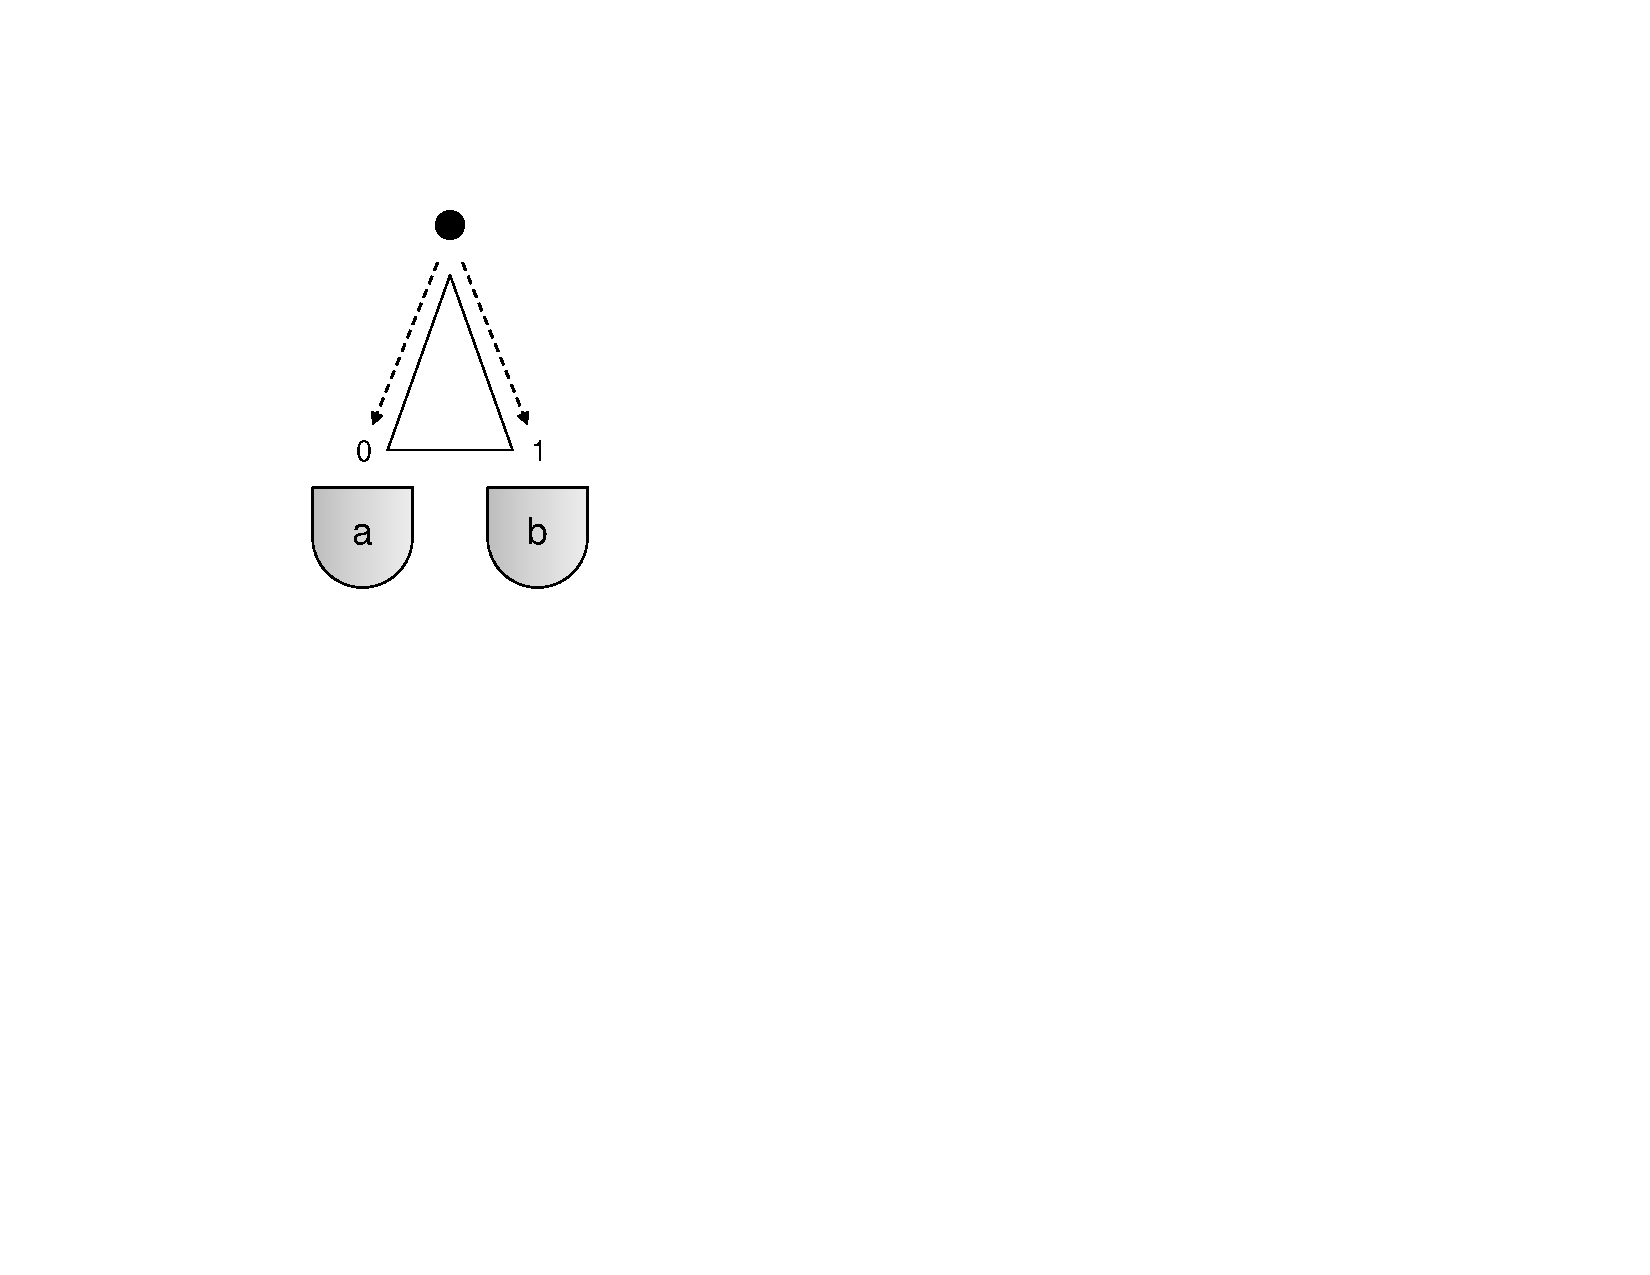
\includegraphics[scale=0.6]{figures/fig-ch6-em-marble1.pdf}
\vspace{-0.3cm}
\end{center}\caption{A simple marble game where a released marble takes one of two possible paths.  This game can be modeled using a Bernoulli random variable with parameter $p$, which indicates the probability that the marble will go to the right when it hits the peg.}\label{chapter6_figure_plinko}
\end{figure*}

To estimate the parameter $p$ of the statistical model of our game, we
need some \emph{training data}, so we drop 10 marbles into the game
which end up in cups $\textbf{x} = \langle
b,b,b,a,b,b,b,b,b,a\rangle$.

What is the maximum likelihood estimate of $p$ given this data?  By
assuming that our samples are independent and identically distributed
(i.i.d.), we can write the likelihood of our data as
follows:\footnote{In this equation, $\delta$ is the Kroneker delta
  function which evaluates to 1 where its arguments are equal and 0
  otherwise.}

\begin{eqnarray*}
\Pr(\textbf{x};p) & = & \prod_{j=1}^{10} p^{\delta(x_j,a)}(1-p)^{\delta(x_j,b)} \\
&  =  & p^2 \cdot (1 - p)^8
\end{eqnarray*}

\noindent Since $\log$ is a monotonically increasing function,
maximizing $\log \Pr(\textbf{x};p)$ will give us the desired result.
We can do this differentiating with respect to $p$ and finding where
the resulting expression equals 0:

\begin{eqnarray*}
\frac{d \log \Pr(\textbf{x};p)}{dp} & = & 0\\
\frac{d [ 2\cdot \log p + 8 \cdot \log (1-p) ]}{dp} & = & 0 \\
\frac{2}{p} - \frac{8}{1-p} & = & 0
\end{eqnarray*}

\noindent Solving for $p$ yields $0.2$, which is the intuitive result.
Furthermore, it is straightforward to show that in $N$ trials where
$N_0$ marbles followed path 0 to cup $a$, and $N_1$ marbles followed
path 1 to cup $b$, the maximum likelihood estimate of $p$ is $N_1 /
(N_0 + N_1)$.

While this model only makes use of an approximation of the true
physical process at work when the marble interacts with the game
board, it is an empirical question whether the model works well enough
in practice to be useful.  Additionally, while a Bernoulli trial is an
extreme approximation of the physical process, if insufficient
resources were invested in building a physical model, the
approximation may perform better than the more complicated
``rule-based'' model.  This sort of dynamic is found often in text
processing problems:\ given enough data, astonishingly simple models
can outperform complex knowledge-intensive models that attempt to
simulate complicated processes.

\subsection{A Latent Variable Marble Game}
\label{chapter6_em_example}

To see where latent variables might come into play in modeling,
consider a more complicated variant of our marble game shown in
Figure~\ref{chapter6_figure_plinko2}.  This version consists of three
pegs that influence the marble's path, and the marble may end up in
one of three cups.  Note that both paths 1 and 2 lead to cup $b$.

\begin{figure*}[t]
\begin{center}
\vspace{0.2cm}
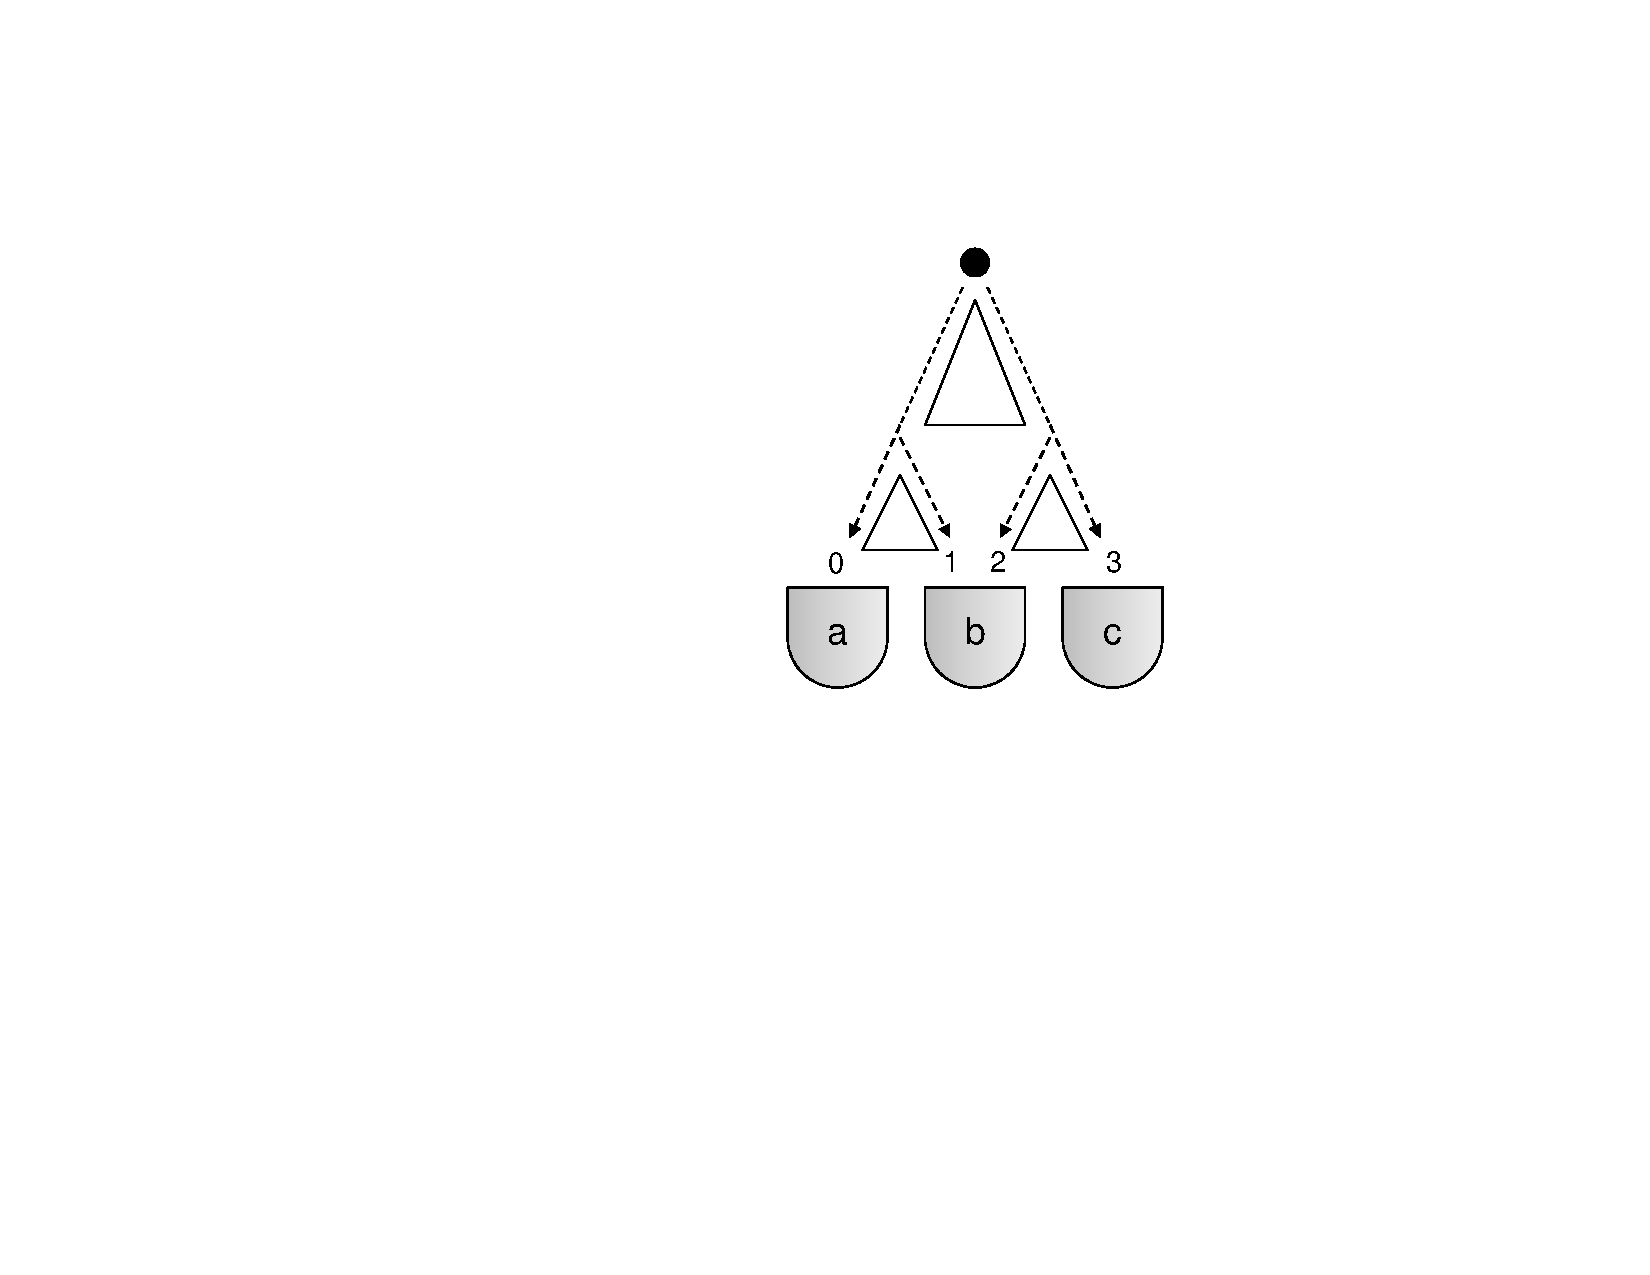
\includegraphics[scale=0.6]{figures/fig-ch6-em-marble2.pdf}
\vspace{-0.3cm}
\end{center}\caption{A more complicated marble game where the released marble takes one of four possible paths.  We assume that we can only observe which cup the marble ends up in, not the specific path taken.}\label{chapter6_figure_plinko2}
\end{figure*}

To construct a statistical model of this game, we again assume that
the behavior of a marble interacting with a peg can be modeled with a
Bernoulli random variable.  Since there are three pegs, we have three
random variables with parameters $\theta=\langle p_0, p_1, p_2
\rangle$, corresponding to the probabilities that the marble will go
to the right at the top, left, and right pegs.  We further define a
random variable $X$ taking on values from $\{a,b,c\}$ indicating what
cup the marble ends in, and $Y$, taking on values from $\{0,1,2,3\}$
indicating which path was taken.  Note that the full joint
distribution $\Pr(X=x,Y=y)$ is determined by $\theta$.

How should the parameters $\theta$ be estimated?  If it were possible
to observe the paths taken by marbles as they were dropped into the
game, it would be trivial to estimate the parameters for our model
using the maximum likelihood estimator---we would simply need to count
the number of times the marble bounced left or right at each peg.  If
$N_x$ counts the number of times a marble took path $x$ in $N$ trials,
this is:

\begin{equation}
p_0 = \frac{N_2 + N_3}{N} \quad \quad p_1 = \frac{N_1}{N_0 + N_1} \quad \quad  p_2 = \frac{N_3}{N_2 + N_3}
\end{equation}

\noindent However, we wish to consider the case where the paths taken
are \emph{unobservable} (imagine an opaque sheet covering the center
of the game board), but where we can see what cup a marble ends in.
In other words, we want to consider the case where we have
\emph{partial} data.  This is exactly the problem encountered in
unsupervised learning:\ there is a statistical model describing the
relationship between two sets of variables ($X$'s and $Y$'s), and
there is data available from just one of them.  Furthermore, such
algorithms are quite useful in text processing, where latent variables
may describe latent linguistic structures of the observed variables,
such as parse trees or part-of-speech tags, or alignment structures
relating sets of observed variables (see
Section~\ref{chapter6_word_alignment}).

\subsection{MLE with Latent Variables}

Formally, we consider the problem of estimating parameters for
statistical models of the form $\Pr(X,Y;\theta)$ which describe not
only an observable variable $X$ but a latent, or hidden, variable $Y$.

In these models, since only the values of the random variable $X$ are
observable, we define our optimization criterion to be the
maximization of the \emph{marginal} likelihood, that is, summing over
all settings of the latent variable $Y$, which takes on values from
set designated $\mathcal{Y}$:\footnote{For this description, we assume
  that the variables in our model take on discrete values.  Not only
  does this simplify exposition, but discrete models are widely used
  in text processing.} Again, we assume that samples in the training
data $\textbf{x}$ are i.i.d.:

\begin{eqnarray*}
\Pr(X=x) = \sum_{y \in \mathcal{Y}} \Pr(X=x,Y=y ; \theta) \\
\end{eqnarray*}

\noindent For a vector of training observations $\textbf{x} = \langle
x_1,x_2, \ldots, x_{\ell} \rangle $, if we assume the samples are
i.i.d.:

\begin{equation}
\Pr(\textbf{x};\theta) = \prod_{j=1}^{|\textbf{x}|} \sum_{y \in \mathcal{Y}} \Pr(X=x_j,Y=y ; \theta)
\end{equation}

\noindent Thus, the maximum (marginal) likelihood estimate of the
model parameters $\theta^*$ given a vector of i.i.d. observations
$\textbf{x}$ becomes:

\begin{equation}
\theta^* = \arg \max_{\theta} \prod_{j=1}^{|\textbf{x}|} \sum_{y \in \mathcal{Y}} \Pr(X=x_j,Y=y ; \theta)
\end{equation}

\noindent Unfortunately, in many cases, this maximum cannot be
computed analytically, but the iterative hill-climbing approach of
expectation maximization can be used instead.

\subsection{Expectation Maximization}

Expectation maximization (EM) is an iterative algorithm that finds a
successive series of parameter estimates $\theta^{(0)}$,
$\theta^{(1)}$, $\ldots$ that improve the marginal likelihood of the
training data.  That is, EM guarantees:

\begin{equation}
\prod_{j=1}^{|\textbf{x}|} \sum_{y \in \mathcal{Y}} \Pr(X=x_j,Y=y ; \theta^{(i+1)}) \ge \prod_{j=1}^{|\textbf{x}|} \sum_{y \in \mathcal{Y}} \Pr(X=x_j,Y=y ; \theta^{(i)})
\end{equation}

\noindent The algorithm starts with some initial set of parameters
$\theta^{(0)}$ and then updates them using two steps:\ expectation
(E-step), which computes the posterior distribution over the latent
variables given the observable data $\textbf{x}$ and a set of
parameters $\theta^{(i)}$,\footnote{The term `expectation' is used
  since the values computed in terms of the posterior distribution
  $\Pr(\textbf{y}|\textbf{x};\theta^{(i)})$ that are required to solve
  the M-step have the form of an expectation (with respect to this
  distribution).} and maximization (M-step), which computes new
parameters $\theta^{(i+1)}$ maximizing the expected log likelihood of
the joint distribution with respect to the distribution computed in
the E-step.  The process then repeats with these new parameters.  The
algorithm terminates when the likelihood remains
unchanged.\footnote{The final solution is only guaranteed to be a
  \emph{local maximum}, but if the model is fully convex, it will also
  be the global maximum.} In more detail, the steps are as follows:

\paragraph{\textbf{E-step.}}
Compute the posterior probability of each possible hidden variable
assignments $y \in \mathcal{Y}$ for each $x \in \mathcal{X}$ and the
current parameter settings, weighted by the relative frequency with
which $x$ occurs in \textbf{x}.  Call this $q(X=x,Y=y;\theta^{(i)})$
and note that it defines a joint probability distribution over
$\mathcal{X} \times \mathcal{Y}$ in that $\sum_{(x,y) \in \mathcal{X}
  \times \mathcal{Y}} q(x,y) = 1$.

\begin{equation}
q(x,y;\theta^{(i)}) = f(x|\textbf{x}) \cdot \Pr(Y=y|X=x;\theta^{(i)})
= f(x|\textbf{x}) \cdot \frac{\Pr(x,y;\theta^{(i)})}{\sum_{y'}
  \Pr(x,y';\theta^{(i)})}
\end{equation}

\paragraph{\textbf{M-step.}}
Compute new parameter settings that maximize the expected log of the
probability of the joint distribution under the $q$-distribution that
was computed in the E-step:

\begin{eqnarray*}
\theta^{(i+1)} &=& \arg \max_{\theta'} \mathbb{E}_{q(X=x,Y=y;\theta^{(i)})} \log \Pr(X=x,Y=y ; \theta') \\
& = & \arg \max_{\theta'} \sum_{(x,y) \in \mathcal{X} \times \mathcal{Y}} q(X=x,Y=y;\theta^{(i)}) \cdot \log \Pr(X=x,Y=y ; \theta')
\end{eqnarray*}

\noindent We omit the proof that the model with parameters
$\theta^{(i+1)}$ will have equal or greater marginal likelihood on the
training data than the model with parameters $\theta^{(i)}$, but this
is provably true \cite{Jelinek_1997}.

Before continuing, we note that the effective application of
expectation maximization requires that both the E-step and the M-step
consist of tractable computations.  Specifically, summing over the
space of hidden variable assignments must not be intractable.
Depending on the independence assumptions made in the model, this may
be achieved through techniques such as dynamic programming.  However,
some models may require intractable computations.

\subsection{An EM Example}

Let's look at how to estimate the parameters from our latent variable
marble game from Section~\ref{chapter6_em_example} using EM.  We
assume training data $\textbf{x}$ consisting of $N=|\textbf{x}|$
observations of $X$ with $N_a$, $N_b$, and $N_c$ indicating the number
of marbles ending in cups $a$, $b$, and $c$.  We start with some
parameters $\theta^{(0)}=\langle p_0^{(0)}, p_1^{(0)}, p_2^{(0)}
\rangle$ that have been randomly initialized to values between 0 and
1.

\paragraph{\textbf{E-step.}}
We need to compute the distribution $q(X=x,Y=y;\theta^{(i)})$, as
defined above.  We first note that the relative frequency
$f(x|\textbf{x})$ is:

\begin{eqnarray*}
f(x|\textbf{x}) = \frac{N_x}{N}
\end{eqnarray*}

\noindent Next, we observe that $\Pr(Y=0|X=a)=1$ and $\Pr(Y=3|X=c)=1$
since cups $a$ and $c$ fully determine the value of the path variable
$Y$.  The posterior probability of paths 1 and 2 are only non-zero
when $X$ is $b$:

\begin{equation}
\Pr(1|b;\theta^{(i)}) = \frac{(1-p_0^{(i)}) p_1^{(i)}}{(1-p_0^{(i)}) p_1^{(i)} + p_0^{(i)} (1-p_2^{(i)})} \quad \Pr(2|b;\theta^{(i)}) = \frac{p_0^{(i)} (1-p_2^{(i)})}{(1-p_0^{(i)}) p_1^{(i)} + p_0^{(i)} (1-p_2^{(i)})}
\end{equation}

\noindent Except for the four cases just described, $\Pr(Y=y|X=x)$ is
zero for all other values of $x$ and $y$ (regardless of the value of
the parameters).

\paragraph{\textbf{M-step.}}
We now need to maximize the expectation of $\log \Pr(X,Y;\theta')$
(which will be a function in terms of the three parameter variables)
under the $q$-distribution we computed in the E step.  The non-zero
terms in the expectation are as follows:

\begin{center}
\begin{tabular}{c|c|c|c}
$x$ & $y$ & $q(X=x,Y=y;\theta^{(i)})$ & $\log \Pr(X=x,Y=y;\theta')$ \\
\hline
$a$ & 0 & $N_a/N$ & $\log (1-p'_0) + \log (1 - p'_1)$ \\
$b$ & 1 & $N_b/N \cdot \Pr(1|b;\theta^{(i)}) $ & $\log(1 - p'_0) + \log p'_1$ \\
$b$ & 2 & $N_b/N \cdot \Pr(2|b;\theta^{(i)}) $ & $\log p'_0 + \log (1-p'_2)$ \\
$c$ & 3 & $N_c/N$ & $\log p'_0 + \log p'_2$ \\
\end{tabular}
\end{center}

\noindent Multiplying across each row and adding from top to bottom
yields the expectation we wish to maximize.  Each parameter can be
optimized independently using differentiation.  The resulting optimal
values are expressed in terms of the counts in $\textbf{x}$ and
$\theta^{(i)}$:

\begin{equation}
p_0 = \frac{\Pr(2|b;\theta^{(i)}) \cdot N_b + N_c}{N} \quad\  p_1 = \frac{\Pr(1|b;\theta^{(i)}) \cdot N_b}{N_a + \Pr(1|b;\theta^{(i)}) \cdot N_b} \quad\   p_2 = \frac{N_c}{\Pr(2|b;\theta^{(i)}) \cdot N_b + N_c}
\end{equation}

\noindent It is worth noting that the form of these expressions is
quite similar to the fully observed maximum likelihood estimate.
However, rather than depending on \emph{exact} path counts, the
statistics used are the \emph{expected} path counts, given
$\textbf{x}$ and parameters $\theta^{(i)}$.

Typically, the values computed at the end of the M-step would serve as
new parameters for another iteration of EM.  However, the example we
have presented here is quite simple and the model converges to a
global optimum after a single iteration.  For most models, EM requires
several iterations to converge, and it may not find a global optimum.
And since EM only finds a locally optimal solution, the final
parameter values depend on the values chose for $\theta^{(0)}$.

\section{Hidden Markov Models}
\label{chapter6_hmms}

To give a more substantial and useful example of models whose
parameters may be estimated using EM, we turn to hidden Markov models
(HMMs).  HMMs are models of data that are ordered \emph{sequentially}
(temporally, from left to right, etc.), such as words in a sentence,
base pairs in a gene, or letters in a word.  These simple but powerful
models have been used in applications as diverse as speech recognition
\cite{Jelinek_1997}, information extraction \cite{Seymore_1999}, gene
finding \cite{Stanke_2003}, part of speech tagging
\cite{Cutting_1992}, stock market forecasting \cite{Hassan_2005}, text
retrieval~\cite{MillerD99}, and word alignment of parallel
(translated) texts \cite{Vogel_1996} (more in
Section~\ref{chapter6_word_alignment}).

In an HMM, the data being modeled is posited to have been generated
from an underlying \emph{Markov process}, which is a stochastic
process consisting of a finite set of states where the probability of
entering a state at time $t+1$ depends only on the state of the
process at time $t$ \cite{Ross_1996}.  Alternatively, one can view a
Markov process as a probabilistic variant of a finite state machine,
where transitions are taken probabilistically.  As another point of
comparison, the PageRank algorithm considered in the previous chapter
(Section~\ref{chapter-graphs:PageRank}) can be understood as a Markov
process:\ the probability of following any link on a particular page
is independent of the path taken to reach that page.  The states of
this Markov process are, however, not directly observable (i.e., \emph{
  hidden}).  Instead, at each time step, an observable token (e.g., a
word, base pair, or letter) is emitted according to a probability
distribution conditioned on the identity of the state that the
underlying process is in.

A hidden Markov model $\mathcal{M}$ is defined as a tuple $\langle
\mathcal{S} , \mathcal{O}, \theta \rangle$.  $\mathcal{S}$ is a finite
set of states, which generate symbols from a finite observation
vocabulary $\mathcal{O}$.  Following convention, we assume that
variables $q$, $r$, and $s$ refer to states in $\mathcal{S}$, and $o$
refers to symbols in the observation vocabulary $\mathcal{O}$. This
model is parameterized by the tuple $\theta=\langle A, B, \pi \rangle$
consisting of an $|\mathcal{S}| \times |\mathcal{S}|$ matrix $A$ of
\emph{transition probabilities}, where $A_{q}(r)$ gives the
probability of transitioning from state $q$ to state $r$; an
$|\mathcal{S}| \times |\mathcal{O}|$ matrix $B$ of \emph{emission
  probabilities}, where $B_{q}(o)$ gives the probability that symbol
$o$ will be emitted from state $q$; and an $|\mathcal{S}|$-dimensional
vector $\pi$, where $\pi_q$ is the probability that the process starts
in state $q$.\footnote{This is only one possible definition of an HMM,
  but it is one that is useful for many text processing problems.  In
  alternative definitions, initial and final states may be handled
  differently, observations may be emitted during the transition
  between states, or continuous-valued observations may be emitted
  (for example, from a Gaussian distribution).}  These matrices may be
dense, but for many applications sparse parameterizations are useful.
We further stipulate that $A_{q}(r) \ge 0$, $B_q(o) \ge 0$, and $\pi_q
\ge 0$ for all $q$, $r$, and $o$, as well as that:

\begin{equation}
\sum_{r \in \mathcal{S}} A_{q}(r) = 1\ \forall q  \quad \quad \sum_{o \in \mathcal{O}} B_{q}(o) = 1\ \forall q   \quad \quad \sum_{q \in \mathcal{S}} \pi_q = 1 
\end{equation}

\noindent A sequence of observations of length $\tau$ is generated as follows:

\begin{itemize}

\item[] Step 0, let $t=1$ and select an initial state $q$ according to the distribution $\pi$.  

\item[] Step 1, an observation symbol from $\mathcal{O}$ is emitted according to the distribution $B_q$. 

\item[] Step 2, a new $q$ is drawn according to the distribution $A_q$.  

\item[] Step 3, $t$ is incremented, and if $t \le \tau$, the process repeats from Step 1.

\end{itemize}

\noindent Since all events generated by this process are conditionally
independent, the joint probability of this sequence of observations
and the state sequence used to generate it is the product of the
individual event probabilities.

Figure~\ref{chapter6_hmm_example} shows a simple example of a hidden
Markov model for part-of-speech tagging, which is the task of
assigning to each word in an input sentence its grammatical category
(one of the first steps in analyzing textual content).  States
$\mathcal{S} = \{ \textsc{det}, \textsc{adj}, \textsc{nn}, \textsc{v}
\}$ correspond to the parts of speech (determiner, adjective, noun,
and verb), and observations $\mathcal{O} = \{ \texttt{the},
\texttt{a}, \texttt{green} , \ldots \}$ are a subset of English words.
This example illustrates a key intuition behind many applications of
HMMs:\ states correspond to equivalence classes or clustering of
observations, and a single observation type may associated with
several clusters (in this example, the word \texttt{wash} can be
generated by an \textsc{nn} or \textsc{v}, since wash can either be a
noun or a verb).

\begin{figure*}
\begin{center}
\vspace{0.2cm}
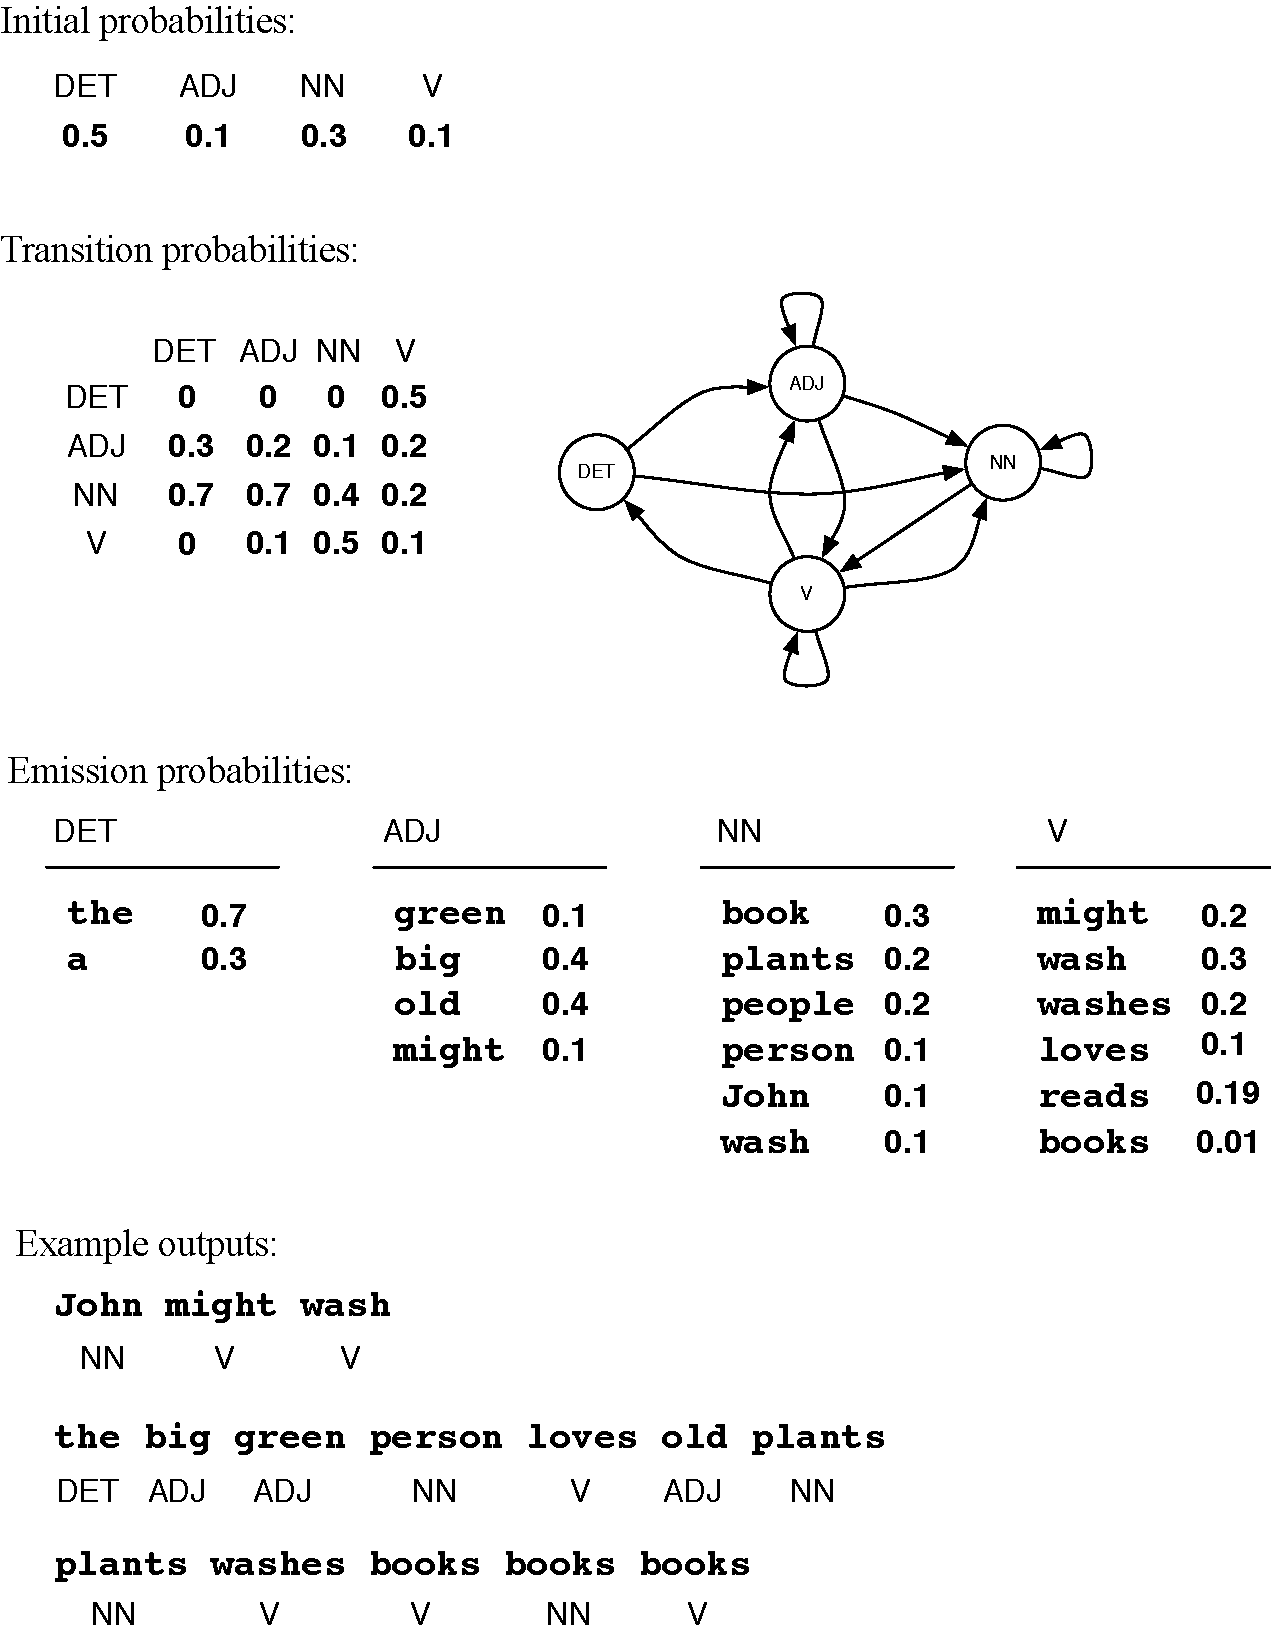
\includegraphics[scale=0.58]{figures/fig-ch6-english-pos-hmm.pdf}
\vspace{-0.3cm}
\end{center}\caption{An example HMM that relates part-of-speech tags to vocabulary items in an English-like language.  Possible (probability $>0$) transitions for the Markov process are shown graphically. In the example outputs, the state sequences corresponding to the emissions are written beneath the emitted symbols.}\label{chapter6_hmm_example}
\end{figure*}

\subsection{Three Questions for Hidden Markov Models}

There are three fundamental questions associated with hidden Markov
models:\footnote{The organization of this section is based in part on
  ideas from Lawrence Rabiner's HMM tutorial \cite{Rabiner_1990}.}

\begin{enumerate}
\item Given a model $\mathcal{M} = \langle \mathcal{S}, \mathcal{O}, \theta \rangle$, and an observation sequence of symbols from $\mathcal{O}$, $\textbf{x} = \langle x_1 , x_2 , \ldots , x_{\tau} \rangle$, what is the probability that $\mathcal{M}$ generated the data (summing over all possible state sequences, $\mathcal{Y}$)?
\begin{equation}
\Pr(\textbf{x}) = \sum_{\textbf{y} \in \mathcal{Y}}\Pr(\textbf{x},\textbf{y};\theta)
\end{equation}
\item Given a model $\mathcal{M} = \langle \mathcal{S}, \mathcal{O}, \theta \rangle$ and an observation sequence $\textbf{x}$, what is the most likely sequence of states that generated the data?
\begin{equation}
\textbf{y}^* = \arg \max_{\textbf{y} \in \mathcal{Y}} \Pr(\textbf{x},\textbf{y};\theta)
\end{equation}
\item Given a set of states $\mathcal{S}$, an observation vocabulary $\mathcal{O}$, and a series of $\ell$ i.i.d. observation sequences $\langle \textbf{x}_1,\textbf{x}_2,\ldots, \textbf{x}_{\ell} \rangle$, what are the parameters $\theta=\langle A, B, \pi \rangle$ that maximize the likelihood of the training data?
\begin{equation}
\theta^* = \arg \max_{\theta} \prod_{i=1}^{\ell} \sum_{\textbf{y} \in \mathcal{Y}} \Pr(\textbf{x}_i,\textbf{y};\theta)
\end{equation}
\end{enumerate}

\noindent Using our definition of an HMM, the answers to the first two
questions are in principle quite trivial to compute:\ by iterating
over all state sequences $\mathcal{Y}$, the probability that each
generated $\textbf{x}$ can be computed by looking up and multiplying
the relevant probabilities in $A$, $B$, and $\pi$, and then summing
the result or taking the maximum. And, as we hinted at in the previous
section, the third question can be answered using EM.  Unfortunately,
even with all the distributed computing power MapReduce makes
available, we will quickly run into trouble if we try to use this
na\"ive strategy since there are $|\mathcal{S}|^{\tau}$ distinct state
sequences of length $\tau$, making exhaustive enumeration
computationally intractable. Fortunately, because the underlying model
behaves exactly the same whenever it is in some state, regardless of
how it got to that state, we can use dynamic programming algorithms to
answer all of the above questions without summing over exponentially
many sequences.

\subsection{The Forward Algorithm}
\label{chapter6_forward}

Given some observation sequence, for example $\textbf{x} = \langle
\texttt{John}, \texttt{might}, \texttt{wash} \rangle$, Question 1 asks
what is the probability that this sequence was generated by an HMM
$\mathcal{M} = \langle \mathcal{S}, \mathcal{O}, \theta \rangle$.  For
the purposes of illustration, we assume that $\mathcal{M}$ is defined
as shown in Figure~\ref{chapter6_hmm_example}.

There are two ways to compute the probability of $\textbf{x}$ having
been generated by $\mathcal{M}$.  The first is to compute the sum over
the joint probability of $\textbf{x}$ and every possible labeling
$\textbf{y}' \in \{ \langle \textsc{det} , \textsc{det}, \textsc{det}
\rangle, \langle \textsc{det} , \textsc{det}, \textsc{nn} \rangle,
\langle \textsc{det} , \textsc{det}, \textsc{v} \rangle , \ldots \}$.
As indicated above this is not feasible for most sequences, since the
set of possible labels is exponential in the length of $\textbf{x}$.
The second, fortunately, is much more efficient.

We can make use of what is known as the \emph{forward algorithm} to
compute the desired probability in polynomial time.  We assume a model
$\mathcal{M} = \langle \mathcal{S}, \mathcal{O}, \theta \rangle$ as
defined above.  This algorithm works by recursively computing the
answer to a related question:\ what is the probability that the
process is in state $q$ at time $t$ and has generated $\langle x_1,
x_2, \ldots , x_t \rangle$?  Call this probability $\alpha_t(q)$.
Thus, $\alpha_t(q)$ is a two dimensional matrix (of size $|\textbf{x}|
\times |\mathcal{S}|$), called a \emph{trellis}.  It is easy to see
that the values of $\alpha_1(q)$ can be computed as the product of two
independent probabilities:\ the probability of starting in state $q$
and the probability of state $q$ generating $x_1$:

\begin{eqnarray*}
\alpha_1(q) = \pi_q \cdot B_q(x_1)
\end{eqnarray*}

\noindent From this, it's not hard to see that the values of
$\alpha_2(r)$ for every $r$ can be computed in terms of the
$|\mathcal{S}|$ values in $\alpha_1(\cdot)$ and the observation $x_2$:

\begin{eqnarray*}
\alpha_2(r) =  B_r(x_2) \cdot \sum_{q \in \mathcal{S}} \alpha_1(q) \cdot A_q(r)
\end{eqnarray*}

\noindent This works because there are $|\mathcal{S}|$ different ways
to get to state $r$ at time $t=2$:\ starting from state
$1,2,\ldots,|\mathcal{S}|$ and transitioning to state $r$.
Furthermore, because the behavior of a Markov process is determined
only by the state it is in at some time (not by how it got to that
state), $\alpha_t(r)$ can always be computed in terms of the
$|\mathcal{S}|$ values in $\alpha_{t-1}(\cdot)$ and the observation
$x_t$:

\begin{eqnarray*}
\alpha_t(r) & = & B_r(x_t) \cdot \sum_{q \in \mathcal{S}} \alpha_{t-1}(q) \cdot A_q(r)  \\
\end{eqnarray*}

\noindent We have now shown how to compute the probability of being in
any state $q$ at any time $t$, having generated $\langle x_1, x_2,
\ldots , x_t \rangle$, with the forward algorithm.  The probability of
the full sequence is the probability of being in time $|\textbf{x}|$
and in \emph{any} state, so the answer to Question 1 can be computed
simply by summing over $\alpha$ values at time $|\textbf{x}|$ for all
states:

\begin{equation}
\Pr(\textbf{x};\theta) = \sum_{q \in \mathcal{S}} \alpha_{|\textbf{x}|}(q)
\end{equation}

\noindent In summary, there are two ways of computing the probability
that a sequence of observations $\textbf{x}$ was generated by
$\mathcal{M}$:\ exhaustive enumeration with summing and the forward
algorithm.  Figure~\ref{chapter6_fig_question1} illustrates the two
possibilities.  The upper panel shows the na\"{i}ve exhaustive
approach, enumerating all $4^3$ possible labels $\textbf{y}'$ of
$\textbf{x}$ and computing their joint probability
$\Pr(\textbf{x},\textbf{y}')$.  Summing over all $\textbf{y}'$, the
marginal probability of $\textbf{x}$ is found to be $0.00018$. The
lower panel shows the forward trellis, consisting of $4 \times 3$
cells.  Summing over the final column also yields $0.00018$, the same
result.

\begin{figure*}
\begin{center}
\vspace{0.2cm}
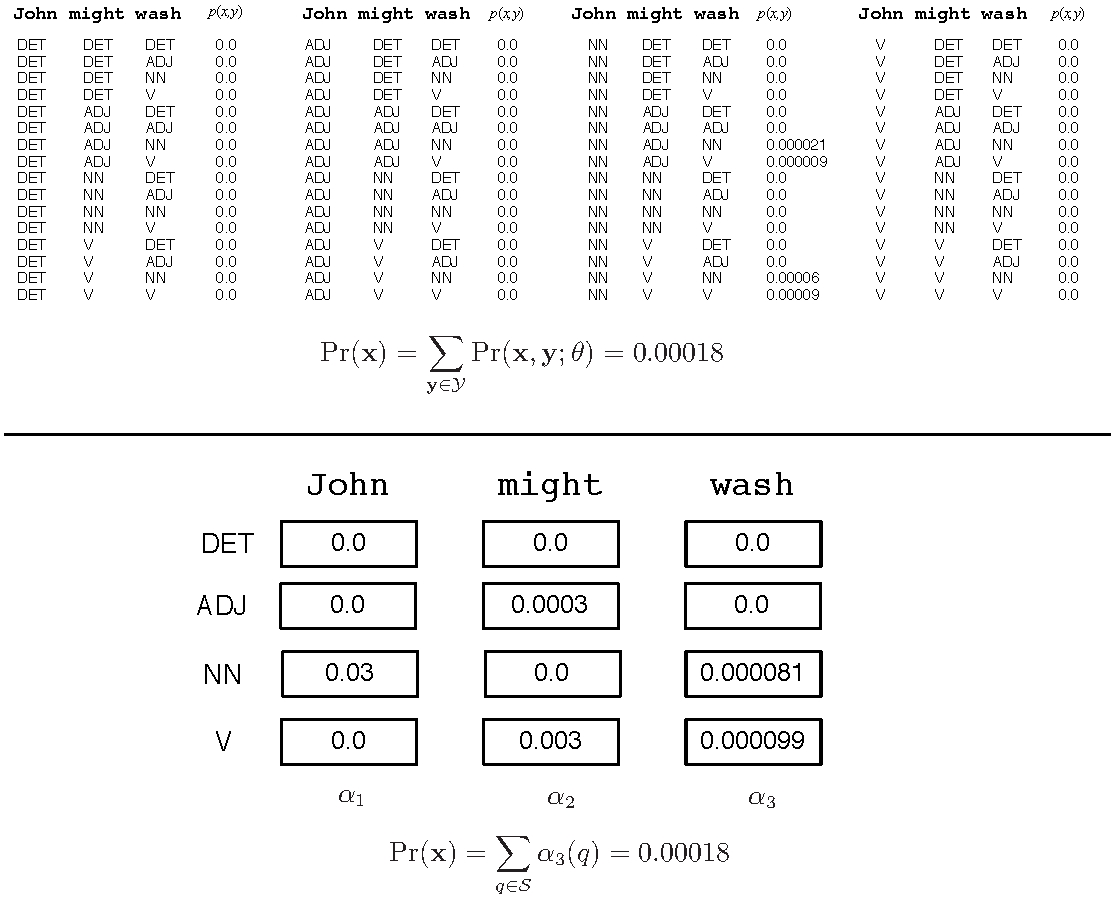
\includegraphics[scale=0.72]{figures/fig-ch6-q1.pdf}
\vspace{-0.3cm}
\end{center}\caption{Computing the probability of the sequence $\langle \texttt{John} , \texttt{might} , \texttt{wash} \rangle$ under the HMM given in Figure~\ref{chapter6_hmm_example} by explicitly summing over all possible sequence labels (upper panel) and using the forward algorithm (lower panel).}\label{chapter6_fig_question1}
\end{figure*}

\subsection{The Viterbi Algorithm}

Given an observation sequence $\mathbf{x}$, the second question we
might want to ask of $\mathcal{M}$ is:\ what is the most likely
sequence of states that generated the observations?  As with the
previous question, the na\"{i}ve approach to solving this problem is
to enumerate all possible labels and find the one with the highest
joint probability.  Continuing with the example observation sequence
$\textbf{x} = \langle \texttt{John} , \texttt{might} , \texttt{wash}
\rangle$, examining the chart of probabilities in the upper panel of
Figure~\ref{chapter6_fig_question1} shows that $\textbf{y}^* = \langle
\textsc{nn}, \textsc{v}, \textsc{v} \rangle$ is the most likely
sequence of states under our example HMM.

However, a more efficient answer to Question 2 can be computed using
the same intuition in the forward algorithm:\ determine the best state
sequence for a short sequence and extend this to easily compute the
best sequence for longer ones.  This is known as the \emph{Viterbi
  algorithm}.  We define $\gamma_t(q)$, the Viterbi probability, to be
the most probable sequence of states ending in state $q$ at time $t$
and generating observations $\langle x_1, x_2, \ldots , x_t \rangle$.
Since we wish to be able to reconstruct the sequence of states, we
define $bp_t(q)$, the ``backpointer'', to be the state used in this
sequence at time $t-1$.  The base case for the recursion is as follows
(the state index of $-1$ is used as a placeholder since there is no
previous best state at time $t=1$):

\begin{eqnarray*}
\gamma_1(q) &=& \pi_q \cdot B_q(x_1) \\
bp_1(q) & = & -1
\end{eqnarray*}

\noindent The recursion is similar to that of the forward algorithm,
except rather than summing over previous states, the \emph{maximum}
value of all possible trajectories into state $r$ at time $t$ is
computed.  Note that the backpointer simply records the index of the
originating state---a separate computation is not necessary.

\begin{eqnarray*}
\gamma_t(r) & = & \max_{q \in \mathcal{S}}  \gamma_{t-1}(q)  \cdot A_q(r) \cdot B_r(x_t)  \\
bp_t(r) & = & \arg \max_{q \in \mathcal{S}} \gamma_{t-1}(q)  \cdot A_q(r) \cdot B_r(x_t)
\end{eqnarray*}

\noindent To compute the best sequence of states, $\textbf{y}^*$, the
state with the highest probability path at time $|\textbf{x}|$ is
selected, and then the backpointers are followed, recursively, to
construct the rest of the sequence:

\begin{eqnarray*}
y_{|\textbf{x}|}^*& =& \arg \max_{q \in \mathcal{S}} \gamma_{|\textbf{x}|}(q)\\
y_{t-1}^* &=& bp_t(y_t)
\end{eqnarray*}

\noindent Figure~\ref{chapter6_fig_question2} illustrates a Viterbi
trellis, including backpointers that have been used to compute the
most likely state sequence.

\begin{figure*}[t]
\begin{center}
\vspace{0.2cm}
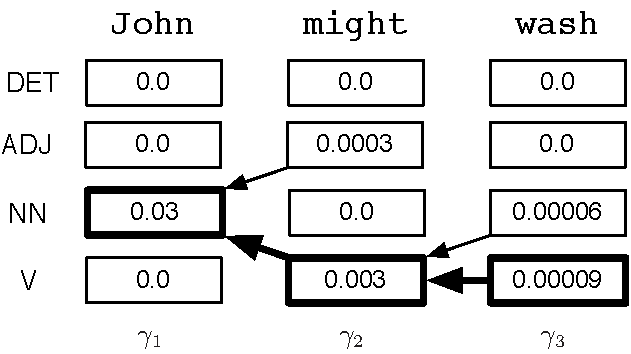
\includegraphics[scale=0.72]{figures/fig-ch6-q2.pdf}
\vspace{-0.3cm}
\end{center}\caption{Computing the most likely state sequence that generated $\langle \texttt{John} , \texttt{might} , \texttt{wash} \rangle$ under the HMM given in Figure~\ref{chapter6_hmm_example} using the Viterbi algorithm.  The most likely state sequence is highlighted in bold and could be recovered programmatically by following backpointers from the maximal probability cell in the last column to the first column (thicker arrows).}\label{chapter6_fig_question2}
\end{figure*}


\subsection{Parameter Estimation for HMMs}
\label{chapter6_forward_backward}

We now turn to Question 3:\ given a set of states $\mathcal{S}$ and
observation vocabulary $\mathcal{O}$, what are the parameters
$\theta^* = \langle A,B,\pi \rangle$ that maximize the likelihood of a
set of training examples, $\langle \textbf{x}_1,\textbf{x}_2,\ldots,
\textbf{x}_{\ell} \rangle$?\footnote{Since an HMM models sequences,
  its training data consists of a collection of example sequences.}
Since our model is constructed in terms of variables whose values we
cannot observe (the state sequence) in the training data, we may train
it to optimize the marginal likelihood (summing over \emph{all} state
sequences) of $\textbf{x}$ using EM.  Deriving the EM update equations
requires only the application of the techniques presented earlier in
this chapter and some differential calculus.  However, since the
formalism is cumbersome, we will skip a detailed derivation, but
readers interested in more information can find it in the relevant
citations \cite{Jelinek_1997,Rabiner_1990}.

\begin{figure*}[t]
\begin{center}
\vspace{0.2cm}
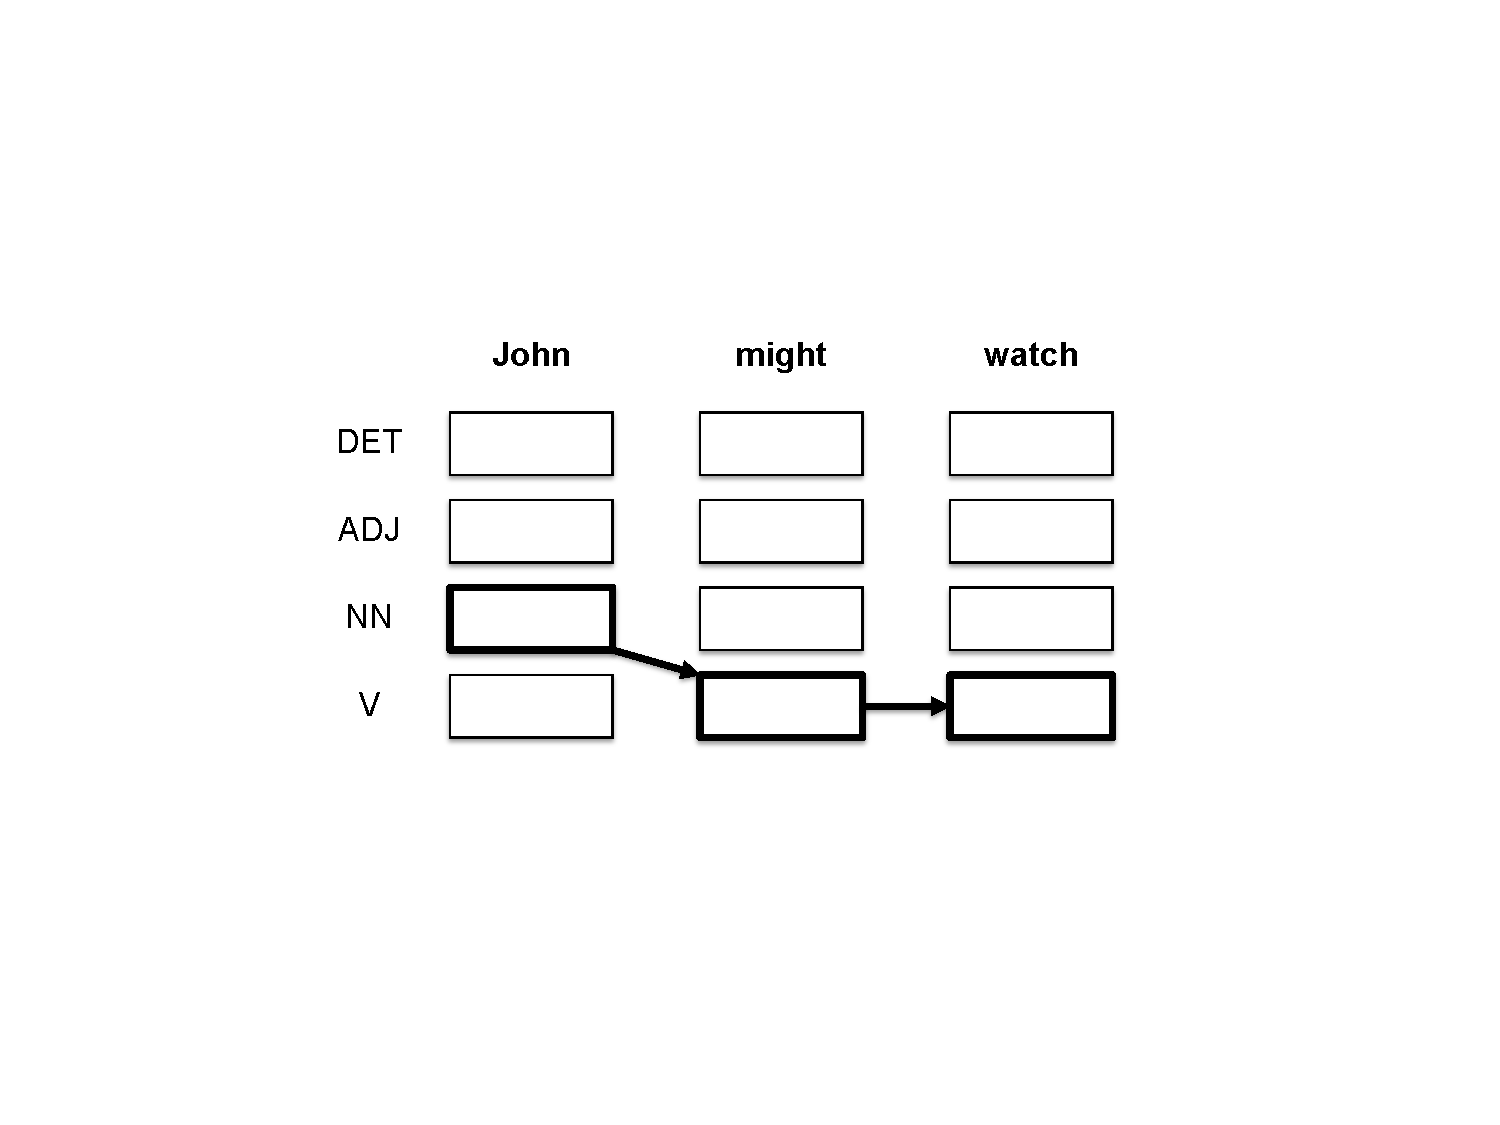
\includegraphics[scale=0.72]{figures/fig-ch6-q3a.pdf}
\vspace{-0.3cm}
\end{center}\caption{A ``fully observable'' HMM training instance.  The output sequence is at the top of the figure, and the corresponding states and transitions are shown in the trellis below.}\label{chapter6_observable_hmm}
\end{figure*}

In order to make the update equations as intuitive as possible,
consider a fully observable HMM, that is, one where both the emissions
and the state sequence are observable in all $\ell$ training
instances.  In this case, a training instance can be depicted as shown
in Figure~\ref{chapter6_observable_hmm}.  When this is the case, such
as when we have a corpus of sentences in which all words have already
been tagged with their parts of speech, the maximum likelihood
estimate for the parameters can be computed in terms of the counts of
the number of times the process transitions from state $q$ to state
$r$ in all training instances, $T(q \rightarrow r)$; the number of
times that state $q$ emits symbol $o$, $O(q \uparrow o)$; and the
number of times the process starts in state $q$, $I(q)$.  In this
example, the process starts in state $\textsc{nn}$; there is one
$\textsc{nn} \rightarrow \textsc{v}$ transition and one $\textsc{v}
\rightarrow \textsc{v}$ transition.  The $\textsc{nn}$ state emits
$\texttt{John}$ in the first time step, and $\textsc{v}$ state emits
$\texttt{might}$ and $\texttt{wash}$ in the second and third time
steps, respectively. We also define $N(q)$ to be the number of times
the process enters state $q$.  The maximum likelihood estimates of the
parameters in the fully observable case are:

\begin{eqnarray}
\label{eq:chapter6_hmmopt} \pi_q = \frac{I(q)}{\ell = \sum_{r} I(r)} \quad \ A_q(r) = \frac{T(q \rightarrow r)}{N(q) = \sum_{r'} T(q \rightarrow r')} \quad\  B_q(o) = \frac{O(q \uparrow o)}{N(q) = \sum_{o'} O(q \uparrow o')}
\end{eqnarray}

\noindent For example, to compute the emission parameters from state
$\textsc{nn}$, we simply need to keep track of the number of times the
process is in state $\textsc{nn}$ and what symbol it generates at each
of these times.  Transition probabilities are computed similarly:\ to
compute, for example, the distribution $A_{\textsc{det}}(\cdot)$, that
is, the probabilities of transitioning away from state $\textsc{det}$,
we count the number of times the process is in state $\textsc{det}$,
and keep track of what state the process transitioned into at the next
time step.  This counting and normalizing be accomplished using the
exact same counting and relative frequency algorithms that we
described in Section~\ref{chapter3:cond-prob}.  Thus, in the fully
observable case, parameter estimation is not a new algorithm at all,
but one we have seen before.

How should the model parameters be estimated when the state sequence
is not provided?  It turns out that the update equations have the
satisfying form where the optimal parameter values for iteration $i+1$
are expressed in terms of the \emph{expectations} of the counts
referenced in the fully observed case, according to the posterior
distribution over the latent variables given the observations
$\textbf{x}$ and the parameters $\theta^{(i)}$:

\begin{equation}
\pi_q = \frac{\mathbb{E}[I(q)]}{\ell} \quad \quad A_q(r) = \frac{\mathbb{E}[T(q \rightarrow r)]}{\mathbb{E}[N(q)]} \quad \quad B_q(o) = \frac{\mathbb{E}[O(q \uparrow o)]}{\mathbb{E}[N(q)]}
\label{chapter6_hmm_update}
\end{equation}

\noindent Because of the independence assumptions made in the HMM, the
update equations consist of $2\cdot |\mathcal{S}| + 1$ independent
optimization problems, just as was the case with the `observable' HMM.
Solving for the initial state distribution, $\pi$, is one problem;
there are $|\mathcal{S}|$ solving for the transition distributions
$A_q(\cdot)$ from each state $q$; and $|\mathcal{S}|$ solving for the
emissions distributions $B_q(\cdot)$ from each state $q$.
Furthermore, we note that the following must hold:

\begin{equation}
\mathbb{E}[N(q)] = \sum_{r \in \mathcal{S}} \mathbb{E}[T(q \rightarrow r)] = \sum_{o \in \mathcal{O}} \mathbb{E}[O(q \uparrow o)]
\end{equation}

\noindent As a result, the optimization problems (i.e.,
Equations~\ref{eq:chapter6_hmmopt}) require completely independent
sets of statistics, which we will utilize later to facilitate
efficient parallelization in MapReduce.

How can the expectations in Equation~\ref{chapter6_hmm_update} be
understood?  In the fully observed training case, between every time
step, there is exactly one transition taken and the source and
destination states are observable.  By progressing through the Markov
chain, we can let each transition count as `1', and we can accumulate
the total number of times each kind of transition was taken (by each
kind, we simply mean the number of times that one state follows
another, for example, the number of times $\textsc{nn}$ follows
$\textsc{det}$).  These statistics can then in turn be used to compute
the MLE for an `observable' HMM, as described above.  However, when
the transition sequence is not observable (as is most often the case),
we can instead imagine that at each time step, \emph{every} possible
transition (there are $|\mathcal{S}|^2$ of them, and typically
$|\mathcal{S}|$ is quite small) is taken, with a particular
probability.  The probability used is the \emph{posterior probability}
of the transition, given the model and an observation sequence (we
describe how to compute this value below).  By summing over all the
time steps in the training data, and using this probability as the
`count' (rather than `1' as in the observable case), we compute the
\emph{expected count} of the number of times a particular transition
was taken, given the training sequence.  Furthermore, since the
training instances are statistically independent, the value of the
expectations can be computed by processing each training instance
independently and summing the results.

Similarly for the necessary emission counts (the number of times each
symbol in $\mathcal{O}$ was generated by each state in $\mathcal{S}$),
we assume that any state could have generated the observation.  We
must therefore compute the probability of being in every state at each
time point, which is then the size of the emission `count'.  By
summing over all time steps we compute the expected count of the
number of times that a particular state generated a particular symbol.
These two sets of expectations, which are written formally here, are
sufficient to execute the M-step.

\begin{eqnarray}
\label{eq:chapter6_ex1} \mathbb{E}[O(q \uparrow o)]& =& \sum_{i=1}^{|\textbf{x}|} \Pr(y_i = q | \textbf{x}; \theta) \cdot \delta(x_i,o) \\
\label{eq:chapter6_ex1a} \mathbb{E}[T(q \rightarrow r)] & = & \sum_{i=1}^{|\textbf{x}|-1} \Pr(y_i = q , y_{i+1} = r | \textbf{x}; \theta)
\end{eqnarray}

\paragraph{\textbf{Posterior probabilities.}}

The expectations necessary for computing the M-step in HMM training
are sums of probabilities that a particular transition is taken, given
an observation sequence, and that some state emits some observation
symbol, given an observation sequence.  These are referred to as
posterior probabilities, indicating that they are the probability of
some event whose distribution we have a prior belief about, after
addition evidence has been taken into consideration (here, the model
parameters characterize our prior beliefs, and the observation
sequence is the evidence).  Both posterior probabilities can be
computed by combining the forward probabilities, $\alpha_t(\cdot)$,
which give the probability of reaching some state at time $t$, by any
path, and generating the observations $\langle x_1, x_2, \ldots , x_t
\rangle$, with \emph{backward probabilities}, $\beta_t(\cdot)$, which
give the probability of starting in some state at time $t$ and
generating the rest of the sequence $\langle x_{t+1}, x_{t+2}, \ldots
, x_{|\textbf{x}|} \rangle$, using any sequence of states to do so.
The algorithm for computing the backward probabilities is given a bit
later.  Once the forward and backward probabilities have been
computed, the state transition posterior probabilities and the
emission posterior probabilities can be written as follows:

\begin{eqnarray}
\label{eq:chapter6_stateocprob} \Pr(y_i = q | \textbf{x}; \theta) & = & \alpha_i(q) \cdot \beta_i(q) \\
\Pr(y_i = q , y_{i+1} = r | \textbf{x}; \theta) & = & \alpha_i(q) \cdot A_q(r) \cdot B_r(x_{i+1}) \cdot \beta_{i+1}(r) \label{eq:chapter6_transprob}
\end{eqnarray}

\noindent Equation~\ref{eq:chapter6_stateocprob} is the probability of
being in state $q$ at time $i$, given $\textbf{x}$, and the
correctness of the expression should be clear from the definitions of
forward and backward probabilities.  The intuition for
Equation~\ref{eq:chapter6_transprob}, the probability of taking a
particular transition at a particular time, is also not
complicated:\ it is the product of four conditionally independent
probabilities:\ the probability of getting to state $q$ at time $i$
(having generated the first part of the sequence), the probability of
taking transition $q \rightarrow r$ (which is specified in the
parameters, $\theta$), the probability of generating observation
$x_{i+1}$ from state $r$ (also specified in $\theta$), and the
probability of generating the rest of the sequence, along any path.  A
visualization of the quantities used in computing this probability is
shown in Figure~\ref{chapter6_forwardbackward}.  In this illustration,
we assume an HMM with $\mathcal{S} = \{ \textsc{s}_1, \textsc{s}_2,
\textsc{s}_3 \}$ and $\mathcal{O}=\{\texttt{a}, \texttt{b}, \texttt{c}
\}$.

\begin{figure*}[t]
\begin{center}
\vspace{0.2cm}
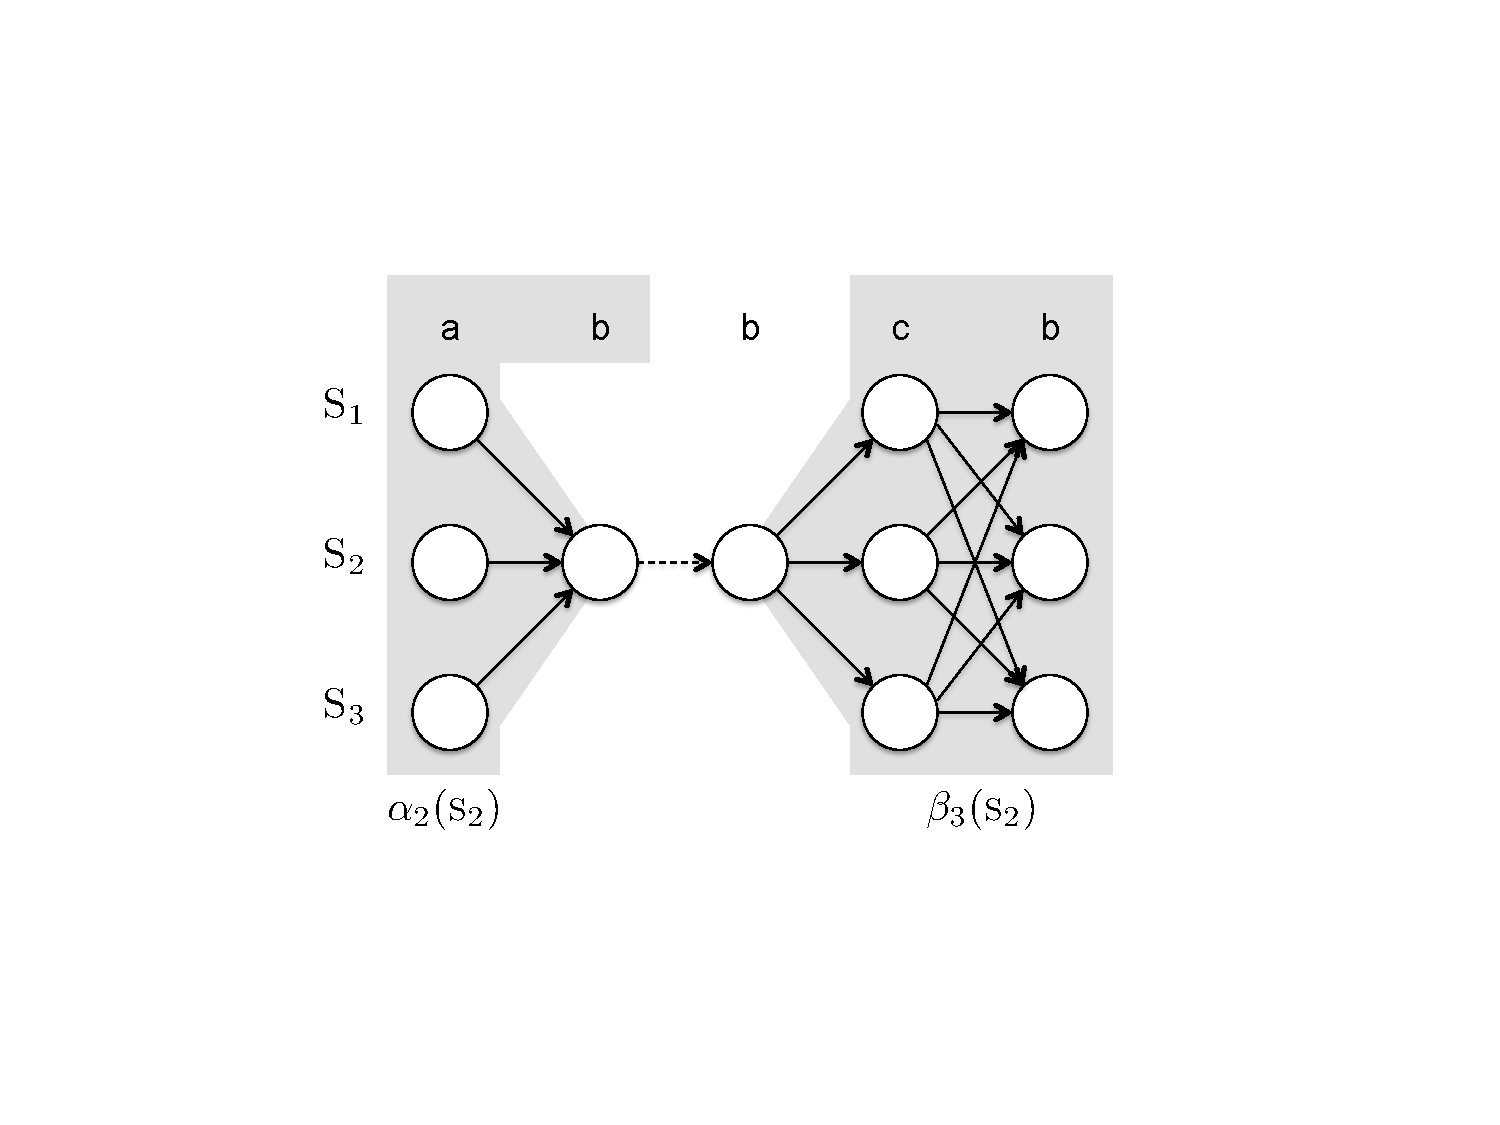
\includegraphics[scale=0.55]{figures/fig-ch6-HMM-forward-backward.pdf}
\vspace{-0.3cm}
\end{center}\caption{Using forward and backward probabilities to compute the posterior probability of the dashed transition, given the observation sequence {\texttt{ a b b c b}.  The shaded area on the left corresponds to the forward probability $\alpha_{2}(\textsc{s}_2)$, and the shaded area on the right corresponds to the backward probability $\beta_3(\textsc{s}_2)$.}\label{chapter6_forwardbackward}}
\end{figure*}

\paragraph{\textbf{The backward algorithm.}}
Like the forward and Viterbi algorithms introduced above to answer
Questions 1 and 2, the backward algorithm uses dynamic programming to
incrementally compute $\beta_t(\cdot)$.  Its base case starts at time
$|\textbf{x}|$, and is defined as follows:

\label{chapter6_backward}

\begin{eqnarray*}
\beta_{|\textbf{x}|}(q) = 1
\end{eqnarray*}

\noindent To understand the intuition for this base case, keep in mind
that since the backward probabilities $\beta_t(\cdot)$ are the
probability of generating the remainder of the sequence \emph{after}
time $t$ (as well as being in some state), and since there is nothing
left to generate after time $|\textbf{x}|$, the probability must be 1.
The recursion is defined as follows:

\begin{eqnarray*}
\beta_{t}(q) = \sum_{r \in \mathcal{S}} \beta_{t+1}(r) \cdot A_q(r) \cdot B_r(x_{t+1})
\end{eqnarray*}

\noindent Unlike the forward and Viterbi algorithms, the backward
algorithm is computed from right to left and makes no reference to the
start probabilities, $\pi$.

\subsection{Forward-Backward Training:\ Summary} 

In the preceding section, we have shown how to compute all quantities
needed to find the parameter settings $\theta^{(i+1)}$ using EM
training with a hidden Markov model $\mathcal{M}=\langle
\mathcal{S},\mathcal{O}, \theta^{(i)} \rangle$.  To recap:\ each
training instance $\textbf{x}$ is processed independently, using the
parameter settings of the current iteration, $\theta^{(i)}$. For each
$\textbf{x}$ in the training data, the forward and backward
probabilities are computed using the algorithms given above (for this
reason, this training algorithm is often referred to as the
forward-backward algorithm).  The forward and backward probabilities
are in turn used to compute the expected number of times the
underlying Markov process enters into each state, the number of times
each state generates each output symbol type, and the number of times
each state transitions into each other state.  These expectations are
summed over all training instances, completing the E-step.  The M-step
involves normalizing the expected counts computed in the E-step using
the calculations in Equation~\ref{chapter6_hmm_update}, which yields
$\theta^{(i+1)}$.  The process then repeats from the E-step using the
new parameters.  The number of iterations required for convergence
depends on the quality of the initial parameters, and the complexity
of the model.  For some applications, only a handful of iterations are
necessary, whereas for others, hundreds may be required.

Finally, a few practical considerations:\ HMMs have a non-convex
likelihood surface (meaning that it has the equivalent of many hills
and valleys in the number of dimensions corresponding to the number of
parameters in the model).  As a result, EM training is only guaranteed
to find a local maximum, and the quality of the learned model may vary
considerably, depending on the initial parameters that are used.
Strategies for optimal selection of initial parameters depend on the
phenomena being modeled.  Additionally, if some parameter is assigned
a probability of 0 (either as an initial value or during one of the
M-step parameter updates), EM will never change this in future
iterations.  This can be useful, since it provides a way of
constraining the structures of the Markov model; however, one must be
aware of this behavior.

Another pitfall to avoid when implementing HMMs is arithmetic
underflow.  HMMs typically define a massive number of sequences, and
so the probability of any one of them is often vanishingly small---so
small that they often underflow standard floating point
representations.  A very common solution to this problem is to
represent probabilities using their logarithms.  Note that expected
counts do not typically have this problem and can be represented using
normal floating point numbers.  See
Section~\ref{chapter-graphs:issues} for additional discussion on
working with log probabilities.

\section{EM in MapReduce}
\label{chapter6_mapreduce}

Expectation maximization algorithms fit quite naturally into the
MapReduce programming model.  Although the model being optimized
determines the details of the required computations, MapReduce
implementations of EM algorithms share a number of characteristics:

\begin{itemize}

\item Each iteration of EM is one MapReduce job.

\item A controlling process (i.e., driver program) spawns the
  MapReduce jobs, keeps track of the number of iterations and
  convergence criteria.

\item Model parameters $\theta^{(i)}$, which are static for the
  duration of the MapReduce job, are loaded by each mapper from HDFS
  or other data provider (e.g., a distributed key-value store).

\item Mappers map over independent training instances, computing
  partial latent variable posteriors (or summary statistics, such as
  expected counts).

\item Reducers sum together the required training statistics
  \emph{and} solve one or more of the M-step optimization problems.

\item Combiners, which sum together the training statistics, are often
  quite effective at reducing the amount of data that must be written
  to disk.

\end{itemize}

\noindent The degree of parallelization that can be attained depends
on the statistical independence assumed in the model and in the
derived quantities required to solve the optimization problems in the
M-step.  Since parameters are estimated from a collection of samples
that are assumed to be i.i.d., the E-step can generally be
parallelized effectively since every training instance can be
processed independently of the others.  In the limit, in fact, each
independent training instance could be processed by a separate
mapper!\footnote{Although the wisdom of doing this is questionable,
  given that the startup costs associated with individual map tasks in
  Hadoop may be considerable.}

Reducers, however, must aggregate the statistics necessary to solve
the optimization problems as required by the model.  The degree to
which these may be solved independently depends on the structure of
the model, and this constrains the number of reducers that may be
used.  Fortunately, many common models (such as HMMs) require solving
several independent optimization problems in the M-step.  In this
situation, a number of reducers may be run in parallel.  Still, it is
possible that in the worst case, the M-step optimization problem will
not decompose into independent subproblems, making it necessary to use
a single reducer.

\subsection{HMM Training in MapReduce}

As we would expect, the training of hidden Markov models parallelizes
well in MapReduce.  The process can be summarized as follows:\ in each
iteration, mappers process training instances, emitting expected event
counts computed using the forward-backward algorithm introduced in
Section~\ref{chapter6_forward_backward}.  Reducers aggregate the
expected counts, completing the E-step, and then generate parameter
estimates for the next iteration using the updates given in
Equation~\ref{chapter6_hmm_update}.

This parallelization strategy is effective for several reasons.
First, the majority of the computational effort in HMM training is the
running of the forward and backward algorithms.  Since there is no
limit on the number of mappers that may be run, the full computational
resources of a cluster may be brought to bear to solve this problem.
Second, since the M-step of an HMM training iteration with
$|\mathcal{S}|$ states in the model consists of $2\cdot |\mathcal{S}|
+ 1$ independent optimization problems that require non-overlapping
sets of statistics, this may be exploited with as many as $2\cdot
|\mathcal{S}| + 1$ reducers running in parallel.  While the
optimization problem is computationally trivial, being able to reduce
in parallel helps avoid the data bottleneck that would limit
performance if only a single reducer is used.

The quantities that are required to solve the M-step optimization
problem are quite similar to the relative frequency estimation example
discussed in Section~\ref{chapter3:cond-prob}; however, rather than
counts of observed events, we aggregate \emph{expected} counts of
events.  As a result of the similarity, we can employ the \emph{
  stripes} representation for aggregating sets of related values, as
described in Section~\ref{chapter3:pairs-and-stripes}.  A \emph{pairs}
approach that requires less memory at the cost of slower performance
is also feasible.

\begin{figure*}[p]
\algrenewcommand\algorithmicfunction{\textbf{class}}
\algrenewcommand\algorithmicprocedure{\textbf{method}}
  \begin{algorithmic}[1]
    \Function{Mapper}{}
    \Procedure{Initialize}{$\textrm{integer \emph{iteration}}$}
    \State $\langle \mathcal{S}, \mathcal{O} \rangle \gets \textsc{ReadModel}$
    \State $\theta \gets \langle A , B , \pi \rangle \gets \textsc{ReadModelParams}(iteration)$
    \EndProcedure
    \Procedure{Map}{$\textrm{sample }id, \textrm{sequence }\textbf{x}$}
        \State $\alpha \gets \textsc{Forward}(\textbf{x},\theta)$ \Comment{\emph{cf.} Section~\ref{chapter6_forward}}
        \State $\beta \gets \textsc{Backward}(\textbf{x},\theta)$ \Comment{\emph{cf.} Section~\ref{chapter6_backward}}
        \State $I \gets \textrm{new }\textsc{AssociativeArray}$ \Comment{Initial state expectations}
        \ForAll{$q \in \mathcal{S}$}   \Comment{Loop over states}
          \State $I\{q\} \gets \alpha_1(q) \cdot \beta_1(q)$
        \EndFor
        
        \State $O \gets \textrm{new }\textsc{AssociativeArray}\textrm{ of }\textsc{AssociativeArray}$ \Comment{Emissions}
        \For{$t = 1$ to $|\textbf{x}|$}  \Comment{Loop over observations}
        \ForAll{$q \in \mathcal{S}$}   \Comment{Loop over states}
           \State $O\{q\}\{x_t\} \gets O\{q\}\{x_t\} + \alpha_t(q) \cdot \beta_t(q)$
        \EndFor
           \State $t \leftarrow t + 1$
        \EndFor

        \State $T \gets \textrm{new }\textsc{AssociativeArray}\textrm{ of }\textsc{AssociativeArray}$\Comment{Transitions}
        \For{$t = 1$ to $|\textbf{x}|-1$}  \Comment{Loop over observations}
        \ForAll{$q \in \mathcal{S}$}   \Comment{Loop over states}
        \ForAll{$r \in \mathcal{S}$}   \Comment{Loop over states}
           \State $T\{q\}\{r\} \gets T\{q\}\{r\} + \alpha_t(q) \cdot A_q(r) \cdot B_r(x_{t+1}) \cdot \beta_{t+1}(r)$
        \EndFor
        \EndFor
        \State $t \leftarrow t + 1$
        \EndFor

        \State $\textsc{Emit}(\textrm{string `\emph{initial}'}, \textrm{stripe }I)$
        \ForAll{$q \in \mathcal{S}$}   \Comment{Loop over states}
           \State $\textsc{Emit}(\textrm{string `\emph{emit from }'}+q, \textrm{stripe }O\{q\})$
           \State $\textsc{Emit}(\textrm{string `\emph{transit from }'}+q, \textrm{stripe }T\{q\})$
        \EndFor

    \EndProcedure
    \EndFunction
  \end{algorithmic}
  \caption{Mapper pseudo-code for training hidden Markov models using EM.  The mappers map over training instances (i.e., sequences of observations $\textbf{x}_i$) and generate the expected counts of initial states, emissions, and transitions taken to generate the sequence.}
\label{figure:chapter6:mr_hmm_mapper}
\end{figure*}

\begin{figure*}[p]
\algrenewcommand\algorithmicfunction{\textbf{class}}
\algrenewcommand\algorithmicprocedure{\textbf{method}}
  \begin{algorithmic}[1]
    \Function{Combiner}{}
    \Procedure{Combine}{$\textrm{string }t, \textrm{stripes }[ C_1, C_2, \ldots ]$}
        \State $C_f \gets \textrm{new }\textsc{AssociativeArray}$
    \ForAll{$ \textrm{stripe }C \in \textrm{stripes }[ C_1, C_2, \ldots ]$}
        \State $\textsc{Sum}(C_f, C)$
    \EndFor
     \State $\textsc{Emit}(\textrm{string }t, \textrm{stripe }C_f)$
    \EndProcedure
    \EndFunction
  \end{algorithmic}
  \begin{algorithmic}[1]
    \Function{Reducer}{}
    \Procedure{Reduce}{$\textrm{string }t, \textrm{stripes }[ C_1, C_2, \ldots ]$}
        \State $C_f \gets \textrm{new }\textsc{AssociativeArray}$
    \ForAll{$ \textrm{stripe }C \in \textrm{stripes }[ C_1, C_2, \ldots ]$}
        \State $\textsc{Sum}(C_f, C)$
    \EndFor
    \State $z \gets 0$
    \ForAll{$\langle k, v \rangle \in C_f$}
	\State $z \gets z + v$
    \EndFor
    \State $P_f \gets \textrm{new }\textsc{AssociativeArray}$\Comment{Final parameters vector}
    \ForAll{$\langle k, v \rangle \in C_f$}
	\State $P_f\{k\} \gets v / z$    
    \EndFor
     \State $\textsc{Emit}(\textrm{string }t, \textrm{stripe }P_f)$
    \EndProcedure
    \EndFunction
  \end{algorithmic}
  \caption{Combiner and reducer pseudo-code for training hidden Markov models using EM. The HMMs considered in this book are fully parameterized by multinomial distributions, so reducers do not require special logic to handle different types of model parameters (since they are all of the same type).}
\label{figure:chapter6:mr_hmm_reducer}
\end{figure*}

\paragraph{\textbf{HMM training mapper.}}
The pseudo-code for the HMM training mapper is given in
Figure~\ref{figure:chapter6:mr_hmm_mapper}.  The input consists of
key-value pairs with a unique id as the key and a training instance
(e.g., a sentence) as the value.  For each training instance, $2n+1$
stripes are emitted with unique keys, and every training instance
emits the same set of keys.  Each unique key corresponds to one of the
independent optimization problems that will be solved in the M-step.
The outputs are:

\begin{enumerate}
\item the probabilities that the unobserved Markov process begins in
  each state $q$, with a unique key designating that the values are
  initial state counts;

\item the expected number of times that state $q$ generated each
  emission symbol $o$ (the set of emission symbols included will be
  just those found in each training instance $\textbf{x}$), with a key
  indicating that the associated value is a set of \emph{emission}
  counts from state $q$; and

\item the expected number of times state $q$ transitions to each state
  $r$, with a key indicating that the associated value is a set of
  \emph{transition} counts from state $q$.

\end{enumerate}

\paragraph{\textbf{HMM training reducer.}}
The reducer for one iteration of HMM training, shown together with an
optional combiner in Figure~\ref{figure:chapter6:mr_hmm_reducer},
aggregates the count collections associated with each key by summing
them.  When the values for each key have been completely aggregated,
the associative array contains all of the statistics necessary to
compute a subset of the parameters for the next EM iteration.  The
optimal parameter settings for the following iteration are computed
simply by computing the relative frequency of each event with respect
to its expected count at the current iteration.  The new computed
parameters are emitted from the reducer and written to HDFS.  Note
that they will be spread across $2\cdot | \mathcal{S} |+1$ keys,
representing initial state probabilities $\pi$, transition
probabilities $A_q$ for each state $q$, and emission probabilities
$B_q$ for each state $q$.


\section{Case Study:\ Word Alignment for Statistical Machine Translation}
\label{chapter6_word_alignment}

To illustrate the real-world benefits of expectation maximization
algorithms using MapReduce, we turn to the problem of word alignment,
which is an important task in statistical machine translation that is
typically solved using models whose parameters are learned with EM.

We begin by giving a brief introduction to statistical machine
translation and the phrase-based translation approach; for a more
comprehensive introduction, refer to \cite{Koehn_2009,Lopez_2008}.
Fully-automated translation has been studied since the earliest days
of electronic computers.  After successes with code-breaking during
World War II, there was considerable optimism that translation of
human languages would be another soluble problem. In the early years,
work on translation was dominated by manual attempts to encode
linguistic knowledge into computers---another instance of the
`rule-based' approach we described in the introduction to this
chapter.  These early attempts failed to live up to the admittedly
optimistic expectations.  For a number of years, the idea of fully
automated translation was viewed with skepticism.  Not only was
constructing a translation system labor intensive, but translation
pairs had to be developed independently, meaning that improvements in
a Russian-English translation system could not, for the most part, be
leveraged to improve a French-English system.

After languishing for a number of years, the field was reinvigorated
in the late 1980s when researchers at IBM pioneered the development of
\emph{statistical machine translation} (SMT), which took a data-driven
approach to solving the problem of machine translation, attempting to
improve both the quality of translation while reducing the cost of
developing systems \cite{Brown_1993}.  The core idea of SMT is to
equip the computer to \emph{learn} how to translate, using example
translations which are produced for other purposes, and modeling the
process as a statistical process with some parameters $\theta$
relating strings in a source language (typically denoted as
$\textbf{f}$) to strings in a target language (typically denoted as
$\textbf{e}$):

\begin{equation}
\textbf{e}^* = \arg \max_{\textbf{e}} \Pr(\textbf{e} | \textbf{f} ; \theta)
\end{equation}

With the statistical approach, translation systems can be developed
cheaply and quickly for any language pair, as long as there is
sufficient training data available.  Furthermore, improvements in
learning algorithms and statistical modeling can yield benefits in
many translation pairs at once, rather than being specific to
individual language pairs.  Thus, SMT, like many other topics we are
considering in this book, is an attempt to leverage the vast
quantities of textual data that is available to solve problems that
would otherwise require considerable manual effort to encode
specialized knowledge. Since the advent of statistical approaches to
translation, the field has grown tremendously and numerous statistical
models of translation have been developed, with many incorporating
quite specialized knowledge about the behavior of natural language as
biases in their learning algorithms.

\subsection{Statistical Phrase-Based Translation}

One approach to statistical translation that is simple yet powerful is
called \emph{phrase-based translation} \cite{Koehn_2003}.  We provide
a rough outline of the process since it is representative of most
state-of-the-art statistical translation systems, such as the one used
inside Google Translate.\footnote{\texttt{http://translate.google.com}}
Phrase-based translation works by learning how strings of words,
called \emph{phrases}, translate between languages.\footnote{Phrases
  are simply sequences of words; they are not required to correspond
  to the definition of a phrase in any linguistic theory.}  Example
phrase pairs for Spanish-English translation might include $\langle
\textrm{\emph{los estudiantes}}, \textrm{\emph{the students}}\rangle$,
$\langle \textrm{\emph{los estudiantes}}, \textrm{\emph{some
    students}}\rangle$, and $\langle \textrm{\emph{soy}},
\textrm{\emph{i am}} \rangle$.  From a few hundred thousand sentences
of example translations, many millions of such phrase pairs may be
automatically learned.

The starting point is typically a parallel corpus (also called \emph{
  bitext}), which contains \emph{pairs} of sentences in two languages
that are translations of each other. Parallel corpora are frequently
generated as the byproduct of an organization's effort to disseminate
information in multiple languages, for example, proceedings of the
Canadian Parliament in French and English, and text generated by the
United Nations in many different languages.  The parallel corpus is
then annotated with \emph{word alignments}, which indicate which words
in one language correspond to words in the other.  By using these word
alignments as a skeleton, phrases can be extracted from the sentence
that is likely to preserve the meaning relationships represented by
the word alignment.  While an explanation of the process is not
necessary here, we mention it as a motivation for learning word
alignments, which we show below how to compute with EM.  After phrase
extraction, each phrase pair is associated with a number of scores
which, taken together, are used to compute the phrase translation
probability, a conditional probability that reflects how likely the
source phrase translates into the target phrase.  We briefly note that
although EM could be utilized to learn the phrase translation
probabilities, this is not typically done in practice since the
maximum likelihood solution turns out to be quite bad for this
problem.  The collection of phrase pairs and their scores are referred
to as the \emph{translation model}.  In addition to the translation
model, phrase-based translation depends on a \emph{language model},
which gives the probability of a string in the target language.  The
translation model attempts to preserve the meaning of the source
language during the translation process, while the language model
ensures that the output is fluent and grammatical in the target
language.  The phrase-based translation process is summarized in
Figure~\ref{chapter6_figure_mtarch}.

\begin{figure*}[p]
\begin{center}
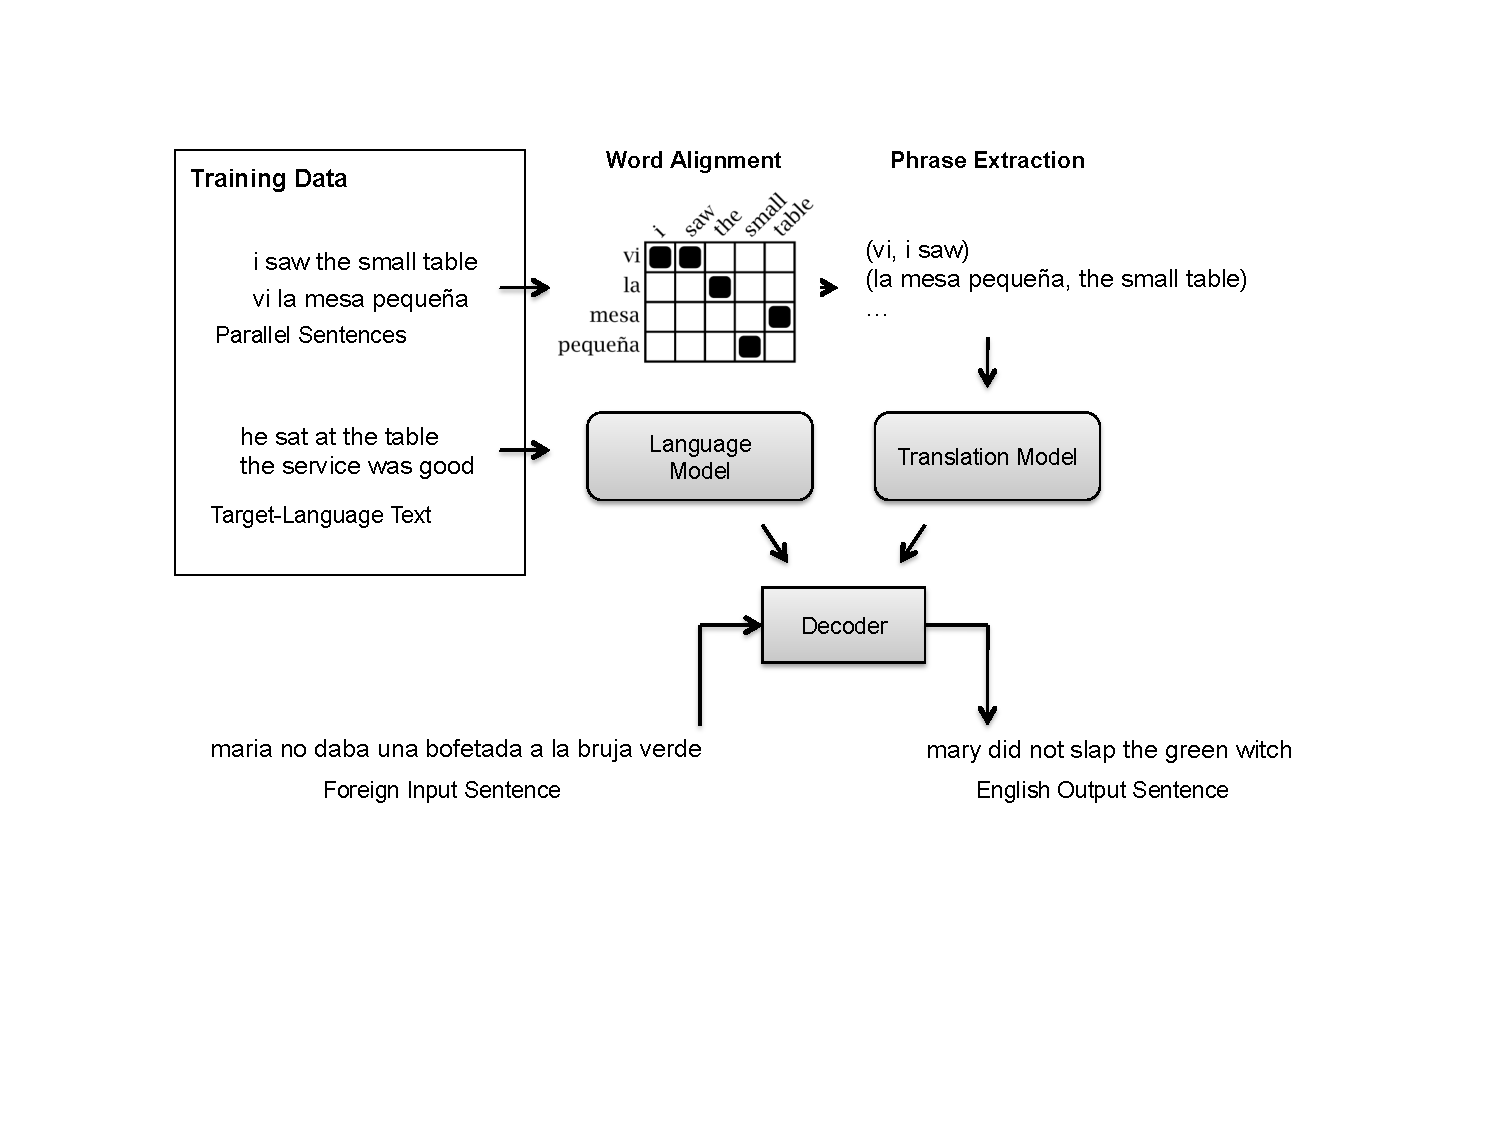
\includegraphics[scale=0.7]{figures/fig-ch6-MT-arch.pdf}
\vspace{-0.3cm}
\end{center}\caption{The standard phrase-based machine translation architecture.  The translation model is constructed with phrases extracted from a word-aligned parallel corpus.  The language model is estimated from a monolingual corpus.  Both serve as input to the decoder, which performs the actual translation.}\label{chapter6_figure_mtarch}
\end{figure*}

\begin{figure*}[p]
\begin{center}
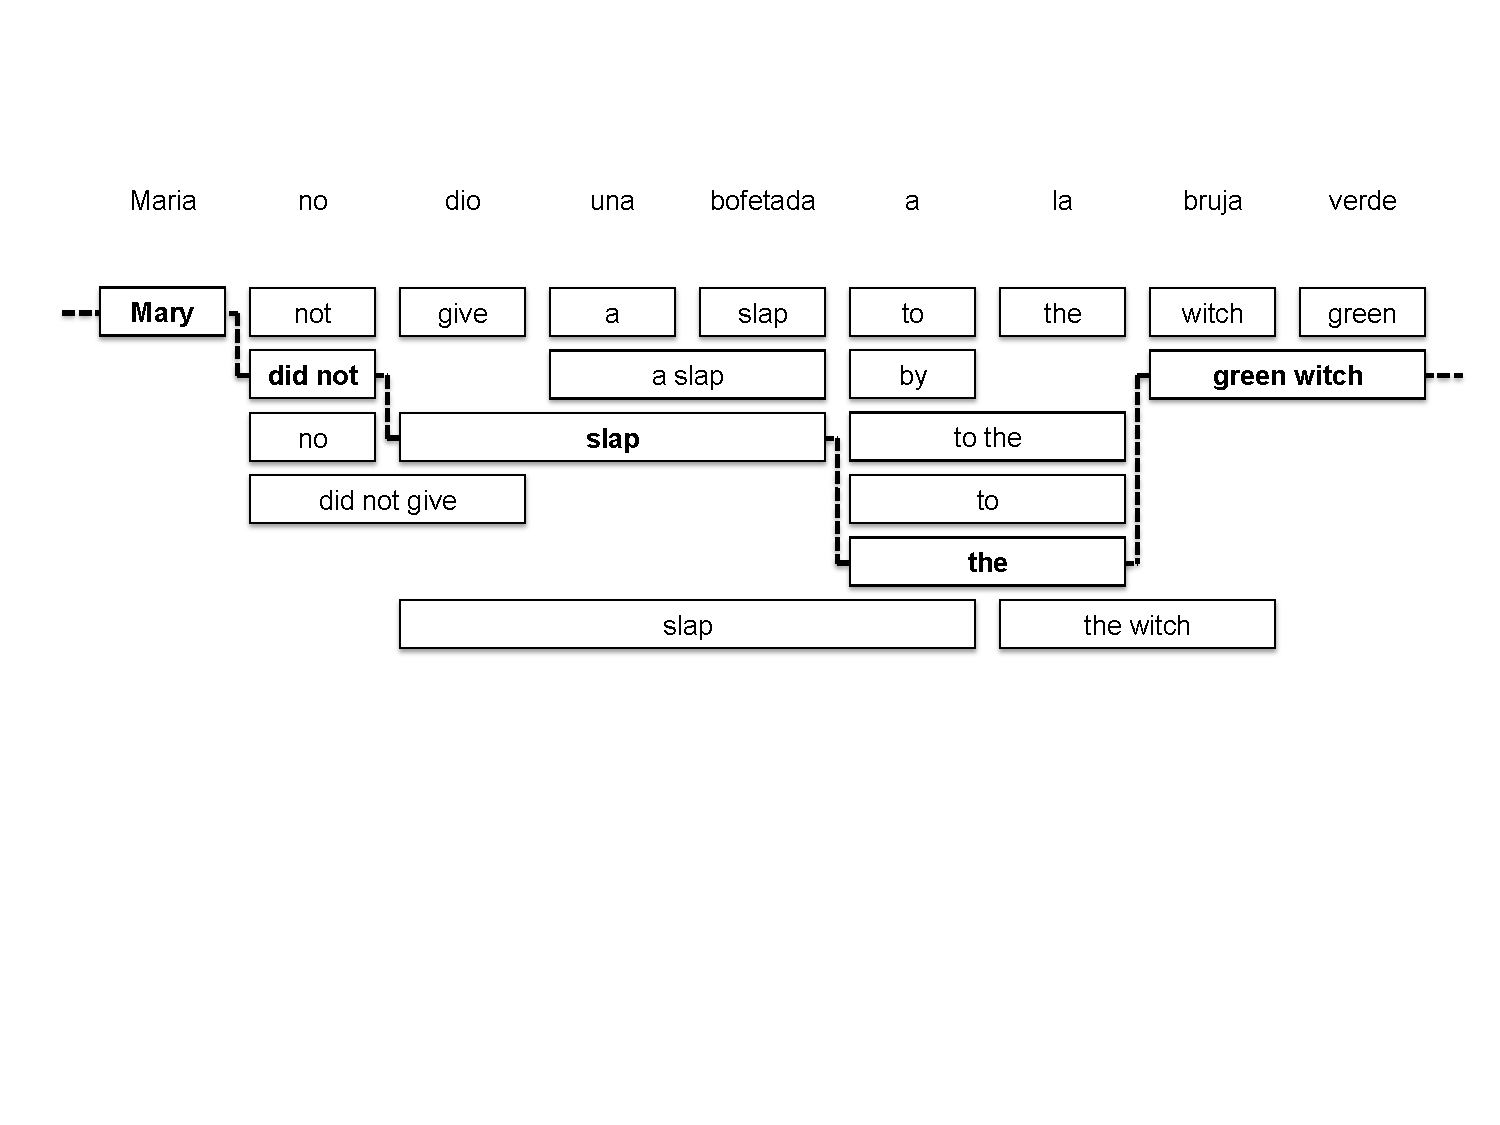
\includegraphics[scale=0.6]{figures/fig-ch6-MT-tiles.pdf}
\vspace{-0.3cm}
\end{center}\caption{Translation coverage of the sentence \emph{Maria no dio una bofetada a la bruja verde} by a phrase-based model. The best possible translation path is indicated with a dashed line.}\label{chapter6_figure_mttiles}
\end{figure*}

A language model gives the probability that a string of words
$\textbf{w} = \langle w_1, w_2, \ldots , w_{n} \rangle$, written as
$w_{1}^{n}$ for short, is a string in the target language.  By the
chain rule of probability, we get:

\begin{equation}
\Pr(w_{1}^{n}) = \Pr(w_1) \Pr(w_2|w_1) \Pr(w_3|w_1^2) \ldots \Pr(w_n|w_1^{n-1}) = \prod_{k=1}^{n} \Pr(w_k|w_1^{k-1})
\end{equation}

\noindent Due to the extremely large number of parameters involved in
estimating such a model directly, it is customary to make the \emph{
  Markov assumption}, that the sequence histories only depend on prior
local context.  That is, an \emph{n}-gram language model is equivalent
to a ($n-1$)\emph{th}-order Markov model.  Thus, we can approximate
$P(w_k|w_1^{k-1})$ as follows:

\begin{eqnarray}
\textrm{bigrams:} & P(w_k|w_1^{k-1}) & \approx P(w_k|w_{k-1}) \\
\textrm{trigrams:} & P(w_k|w_1^{k-1}) & \approx P(w_k|w_{k-1} w_{k-2}) \\
\textrm{\emph{n}-grams:} & P(w_k|w_1^{k-1}) & \approx  P(w_k|w_{k-n+1}^{k-1})
\end{eqnarray}

\noindent The probabilities used in computing $\Pr(w_{1}^{n})$ based
on an \emph{n}-gram language model are generally estimated from a
monolingual corpus of target language text.  Since only target
language text is necessary (without any additional annotation),
language modeling has been well served by large-data approaches that
take advantage of the vast quantities of text available on the web.

To translate an input sentence $\textbf{f}$, the phrase-based
\emph{decoder} creates a matrix of all translation possibilities of
all substrings in the input string, as an example illustrates in
Figure~\ref{chapter6_figure_mttiles}.  A sequence of phrase pairs is
selected such that each word in $\textbf{f}$ is translated exactly
once.\footnote{The phrases may not necessarily be selected in a strict
  left-to-right order.  Being able to vary the order of the phrases
  used is necessary since languages may express the same ideas using
  different word orders.}  The decoder seeks to find the translation
that maximizes the product of the translation probabilities of the
phrases used and the language model probability of the resulting
string in the target language.  Because the phrase translation
probabilities are independent of each other and the Markov assumption
made in the language model, this may be done efficiently using dynamic
programming.  For a detailed introduction to phrase-based decoding, we
refer the reader to a recent textbook by Koehn~\cite{Koehn_2009}.

\subsection{Brief Digression:\ Language Modeling with MapReduce}

Statistical machine translation provides the context for a brief
digression on distributed parameter estimation for language models
using MapReduce, and provides another example illustrating the
effectiveness data-driven approaches in general.  We briefly touched
upon this work in Chapter~\ref{chapter1}.  Even after making the
Markov assumption, training \emph{n}-gram language models still
requires estimating an enormous number of parameters:\ potentially
$V^n$, where $V$ is the number of words in the vocabulary.  For
higher-order models (e.g., 5-grams) used in real-world applications,
the number of parameters can easily exceed the number of words from
which to estimate those parameters.  In fact, most \emph{n}-grams will
never be observed in a corpus, no matter how large.  To cope with this
sparseness, researchers have developed a number of smoothing
techniques~\cite{Manning_Schutze_1999}, which all share the basic idea
of moving probability mass from observed to unseen events in a
principled manner.  For many applications, a state-of-the-art approach
is known as Kneser-Ney smoothing~\cite{Chen_Goodman_ACL1996}.

In 2007, Brants et al.~\cite{Brants_etal_EMNLP2007} reported
experimental results that answered an interesting question:\ given the
availability of large corpora (i.e., the web), could a simpler
smoothing strategy, applied to more text, beat Kneser-Ney in a machine
translation task?  It should come as no surprise that the answer is
\emph{yes}. Brants et al.\ introduced a technique known as ``stupid
backoff'' that was exceedingly simple and so na\"{i}ve that the
resulting model didn't even define a valid probability distribution
(it assigned arbitrary scores as opposed to probabilities).  The
simplicity, however, afforded an extremely scalable implementations in
MapReduce.  With smaller corpora, stupid backoff didn't work as well
as Kneser-Ney in generating accurate and fluent translations.
However, as the amount of data increased, the gap between stupid
backoff and Kneser-Ney narrowed, and eventually disappeared with
sufficient data.  Furthermore, with stupid backoff it was possible to
train a language model on more data than was feasible with Kneser-Ney
smoothing.  Applying this language model to a machine translation task
yielded better results than a (smaller) language model trained with
Kneser-Ney smoothing.

The role of the language model in statistical machine translation is
to select fluent, grammatical translations from a large hypothesis
space:\ the more training data a language model has access to, the
better its description of relevant language phenomena and hence its
ability to select good translations.  Once again, large data triumphs!
For more information about estimating language models using MapReduce,
we refer the reader to a forthcoming book from Morgan \&
Claypool~\cite{Brants_2010}.

\subsection{Word Alignment}

Word alignments, which are necessary for building phrase-based
translation models (as well as many other more sophisticated
translation models), can be learned automatically using EM.  In this
section, we introduce a popular alignment model based on HMMs.

In the statistical model of word alignment considered here, the
observable variables are the words in the source and target sentences
(conventionally written using the variables $\textbf{f}$ and
$\textbf{e}$, respectively), and their alignment is a latent variable.
To make this model tractable, we assume that words are translated
independently of one another, which means that the model's parameters
include the probability of any word in the source language translating
to any word in the target language.  While this independence
assumption is problematic in many ways, it results in a simple model
structure that admits efficient inference yet produces reasonable
alignments.  Alignment models that make this assumption generate a
string $\textbf{e}$ in the target language by selecting words in the
source language according to a lexical translation distribution.  The
indices of the words in $\textbf{f}$ used to generate each word in
$\textbf{e}$ are stored in an alignment variable,
$\textbf{a}$.\footnote{In the original presentation of statistical
  lexical translation models, a special null word is added to the
  source sentences, which permits words to be inserted `out of
  nowhere'.  Since this does not change any of the important details
  of training, we omit it from our presentation for simplicity.} This
means that the variable $a_i$ indicates the source word position of
the $i^{\textrm{\emph{th}}}$ target word generated, and $|\textbf{a}|
= |\textbf{e}|$.  Using these assumptions, the probability of an
alignment and translation can be written as follows:

\begin{eqnarray*}
\Pr(\textbf{e}, \textbf{a} | \textbf{f}) =  \underbrace{  \Pr(\textbf{a} | \textbf{f} , \textbf{e}) }_{\textrm{Alignment probability}} \times  \underbrace{ \prod_{i=1}^{|\textbf{e}|} \Pr(e_i|f_{a_i}) }_{\textrm{Lexical probability}}
\end{eqnarray*}

\noindent Since we have parallel corpora consisting of only $\langle
\textbf{f}, \textbf{e} \rangle$ pairs, we can learn the parameters for
this model using EM and treating $\textbf{a}$ as a latent variable.
However, to combat data sparsity in the alignment probability, we must
make some further simplifying assumptions.  By letting the probability
of an alignment depend only on the position of the previous aligned
word we capture a valuable insight (namely, words that are nearby in
the source language will tend to be nearby in the target language),
and our model acquires the structure of an HMM \cite{Vogel_1996}:

\begin{eqnarray*}
\Pr(\textbf{e}, \textbf{a} | \textbf{f}) & = & \underbrace{\prod_{i=1}^{|\textbf{e}|} \Pr(a_i | a_{i-1})}_{\textrm{Transition probability}} \times \underbrace{\prod_{i=1}^{|\textbf{e}|} \Pr(e_i|f_{a_i})}_{\textrm{Emission probability}} 
\end{eqnarray*}

\noindent This model can be trained using the forward-backward
algorithm described in the previous section, summing over all settings
of $\textbf{a}$, and the best alignment for a sentence pair can be
found using the Viterbi algorithm.

To properly initialize this HMM, it is conventional to further
simplify the alignment probability model, and use this simpler model
to learn initial lexical translation (emission) parameters for the
HMM.  The favored simplification is to assert that all alignments are
uniformly probable:

\begin{eqnarray*}
\Pr(\textbf{e}, \textbf{a} | \textbf{f}) & = & \frac{1}{|\textbf{f}|^{|\textbf{e}|}} \times \prod_{i=1}^{|\textbf{e}|} \Pr(e_i|f_{a_i}) 
\end{eqnarray*}

\noindent This model is known as IBM Model 1.  It is attractive for
initialization because it is convex everywhere, and therefore EM will
learn the same solution regardless of initialization.  Finally, while
the forward-backward algorithm could be used to compute the expected
counts necessary for training this model by setting $A_q(r)$ to be a
constant value for all $q$ and $r$, the uniformity assumption means
that the expected emission counts can be estimated in time
$O(|\textbf{e}| \cdot |\textbf{f}|)$, rather than time $O(|\textbf{e}|
\cdot |\textbf{f}|^2)$ required by the forward-backward algorithm.

\subsection{Experiments}

How well does a MapReduce word aligner for statistical machine
translation perform?  We describe previously-published
results~\cite{Dyer_etal_2008} that compared a Java-based Hadoop
implementation against a highly optimized word aligner called
Giza++~\cite{Och_2003}, which was written in C++ and designed to run
efficiently on a single core.  We compared the training time of Giza++
and our aligner on a Hadoop cluster with 19 slave nodes, each with two
single-core processors and two disks (38 cores total).

Figure~\ref{chapter6_figure_giza_timing} shows the performance of
Giza++ in terms of the running time of a single EM iteration for both
Model 1 and the HMM alignment model as a function of the number of
training pairs.  Both axes in the figure are on a log scale, but the
ticks on the $y$-axis are aligned with `meaningful' time intervals
rather than exact orders of magnitude.  There are three things to
note.  First, the running time scales linearly with the size of the
training data.  Second, the HMM is a constant factor slower than Model
1.  Third, the alignment process is quite slow as the size of the
training data grows---at one million sentences, a single iteration
takes over three hours to complete!  Five iterations are generally
necessary to train the models, which means that full training takes
the better part of a day.

In Figure~\ref{chapter6_figure_mr_timing} we plot the running time of
our MapReduce implementation running on the 38-core cluster described
above.  For reference, we plot points indicating what 1/38 of the
running time of the Giza++ iterations would be at each data size,
which gives a rough indication of what an `ideal' parallelization
could achieve, assuming that there was no overhead associated with
distributing computation across these machines.  Three things may be
observed in the results.  First, as the amount of data increases, the
relative cost of the overhead associated with distributing data,
marshaling and aggregating counts, decreases.  At one million sentence
pairs of training data, the HMM alignment iterations begin to approach
optimal runtime efficiency.  Second, Model 1, which we observe is
light on computation, does not approach the theoretical performance of
an ideal parallelization, and in fact, has almost the same running
time as the HMM alignment algorithm. We conclude that the overhead
associated with distributing and aggregating data is significant
compared to the Model 1 computations, although a comparison with
Figure~\ref{chapter6_figure_giza_timing} indicates that the MapReduce
implementation is still substantially faster than the single core
implementation, at least once a certain training data size is reached.
Finally, we note that, in comparison to the running times of the
single-core implementation, at large data sizes, there is a
significant advantage to using the distributed implementation, even of
Model 1.

Although these results do confound several variables (Java vs. C++
performance, memory usage patterns), it is reasonable to expect that
the confounds would tend to make the single-core system's performance
appear relatively \emph{better} than the MapReduce system (which is,
of course, the opposite pattern from what we actually observe).
Furthermore, these results show that when computation is distributed
over a cluster of many machines, even an unsophisticated
implementation of the HMM aligner could compete favorably with a
highly optimized single-core system whose performance is well-known to
many people in the MT research community.

\begin{figure*}[p]
\begin{center}
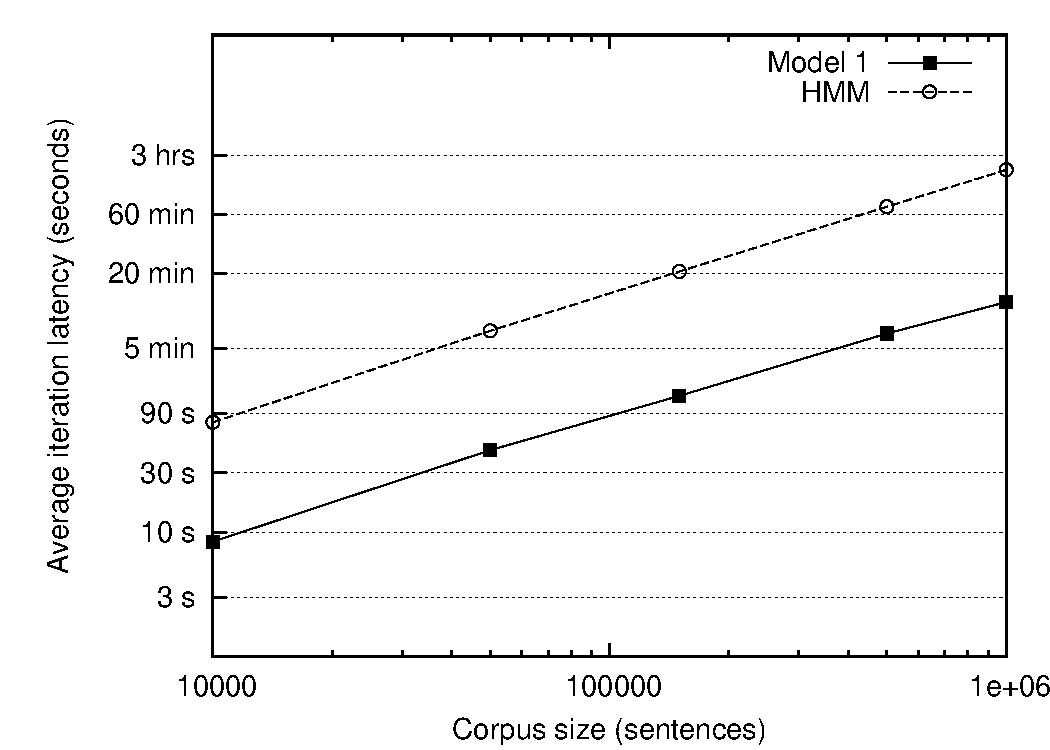
\includegraphics[scale=0.6]{figures/fig-ch6-GIZA-timing.pdf}
\vspace{-0.3cm}
\end{center}\caption{Running times of Giza++ (baseline single-core system) for Model 1 and HMM training iterations at various corpus sizes.}\label{chapter6_figure_giza_timing}
\end{figure*}

\begin{figure*}[p]
\begin{center}
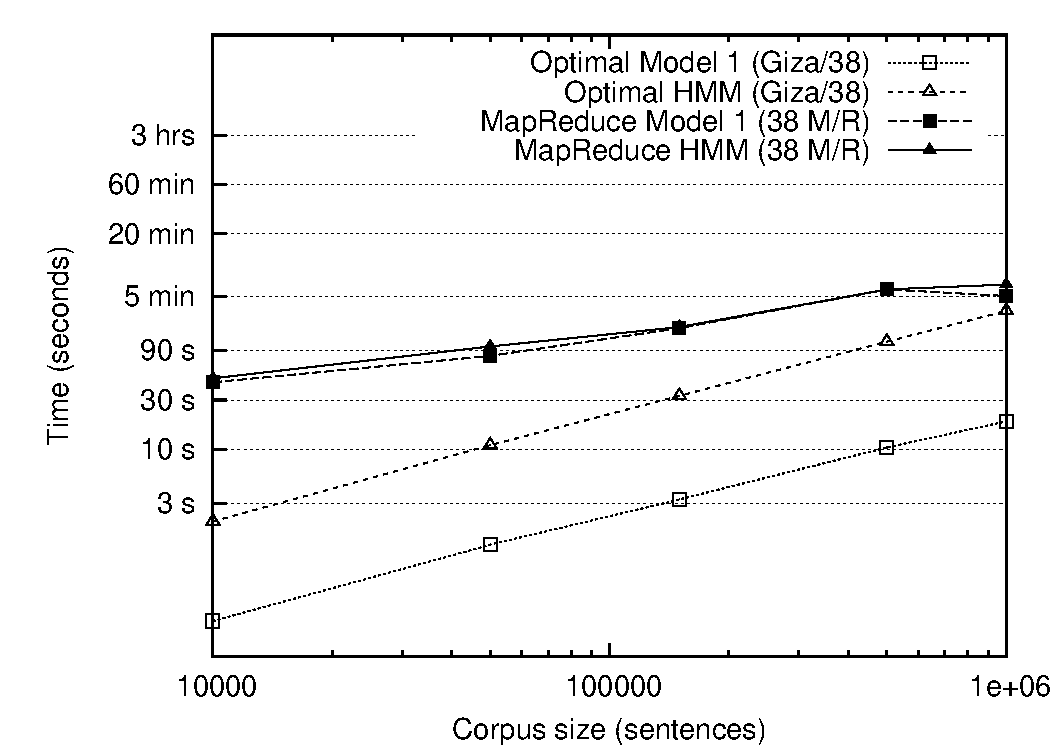
\includegraphics[scale=0.6]{figures/fig-ch6-alignment-timing.pdf}
\vspace{-0.3cm}
\end{center}\caption{Running times of our MapReduce implementation of Model 1 and HMM training iterations at various corpus sizes.  For reference, $1/38$ running times of the Giza++ models are shown.}\label{chapter6_figure_mr_timing}
\end{figure*}

Why are these results important? Perhaps the most significant reason
is that the quantity of parallel data that is available to train
statistical machine translation models is ever increasing, and as is
the case with so many problems we have encountered, more data leads to
improvements in translation quality \cite{Dyer_etal_2008}.  Recently a
corpus of one billion words of French-English data was mined
automatically from the web and released publicly
\cite{Callison_Burch_2009}.\footnote{\texttt{
    http://www.statmt.org/wmt10/translation-task.html}} Single-core
solutions to model construction simply cannot keep pace with the
amount of translated data that is constantly being
produced. Fortunately, several independent researchers have shown that
existing modeling algorithms can be expressed naturally and
effectively using MapReduce, which means that we can take advantage of
this data.  Furthermore, the results presented here show that even at
data sizes that may be tractable on single machines, significant
performance improvements are attainable using MapReduce
implementations.  This improvement reduces experimental turnaround
times, which allows researchers to more quickly explore the solution
space---which will, we hope, lead to rapid new developments in
statistical machine translation.

For the reader interested in statistical machine translation, there is
an open source Hadoop-based MapReduce implementation of a training
pipeline for phrase-based translation that includes word alignment,
phrase extraction, and phrase scoring \cite{Gao_2010}.

\section{EM-Like Algorithms}
\label{chapter6_variants}

This chapter has focused on expectation maximization algorithms and
their implementation in the MapReduce programming framework.  These
important algorithms are indispensable for learning models with latent
structure from unannotated data, and they can be implemented quite
naturally in MapReduce.  We now explore some related learning
algorithms that are similar to EM but can be used to solve more
general problems, and discuss their implementation.

In this section we focus on \emph{gradient-based optimization}, which
refers to a class of techniques used to optimize any objective
function, provided it is differentiable with respect to the parameters
being optimized.  Gradient-based optimization is particularly useful
in the learning of maximum entropy (maxent) models~\cite{Nigam_1999}
and conditional random fields (CRF)~\cite{Lafferty_2001} that have an
exponential form and are trained to maximize conditional likelihood.
In addition to being widely used supervised classification models in
text processing (meaning that during training, both the data and their
annotations must be observable), their gradients take the form of
expectations.  As a result, some of the previously-introduced
techniques are also applicable for optimizing these models.

\subsection{Gradient-Based Optimization and Log-Linear Models}

Gradient-based optimization refers to a class of iterative
optimization algorithms that use the derivatives of a function to find
the parameters that yield a minimal or maximal value of that function.
Obviously, these algorithms are only applicable in cases where a
useful objective exists, is differentiable, and its derivatives can be
efficiently evaluated.  Fortunately, this is the case for many
important problems of interest in text processing.  For the purposes
of this discussion, we will give examples in terms of minimizing
functions.

Assume that we have some real-valued function $F(\theta)$ where
$\theta$ is a $k$-dimensional vector and that $F$ is differentiable
with respect to $\theta$.  Its gradient is defined as:

\begin{equation}
\nabla F(\theta) = \left\langle \frac{\partial F}{\partial \theta_1}(\theta), \frac{\partial F}{\partial \theta_2}(\theta) , \ldots , \frac{\partial F}{\partial \theta_k}(\theta) \right\rangle
\end{equation}

\noindent The gradient has two crucial properties that are exploited
in gradient-based optimization.  First, the gradient $\nabla F$ is a
vector field that points in the direction of the greatest increase of
$F$ and whose magnitude indicates the rate of increase.  Second, if
$\theta^*$ is a (local) minimum of F, then the following is true:

\begin{equation}
\nabla F(\theta^*) = 0
\end{equation}

An extremely simple gradient-based minimization algorithm produces a
series of parameter estimates $\theta^{(1)}, \theta^{(2)}, \ldots$ by
starting with some initial parameter settings $\theta^{(1)}$ and
updating parameters through successive iterations according to the
following rule:

\begin{equation}
\theta^{(i+1)} = \theta^{(i)} - \eta^{(i)} \nabla F(\theta^{(i)})
\label{chapter6_eq_grad_opt1}
\end{equation}

\noindent The parameter $\eta^{(i)} > 0$ is a learning rate which
indicates how quickly the algorithm moves along the gradient during
iteration $i$.  Provided this value is small enough that $F$
decreases, this strategy will find a local minimum of $F$.  However,
while simple, this update strategy may converge slowly, and proper
selection of $\eta$ is non-trivial.  More sophisticated algorithms
perform updates that are informed by approximations of the second
derivative, which are estimated by successive evaluations of $\nabla
F(\theta)$, and can converge much more rapidly \cite{LBFGS}.

\paragraph{\textbf{Gradient-based optimization in MapReduce.}}
Gradient-based optimization algorithms can often be implemented
effectively in MapReduce.  Like EM, where the structure of the model
determines the specifics of the realization, the details of the
function being optimized determines how it should best be implemented,
and not every function optimization problem will be a good fit for
MapReduce.  Nevertheless, MapReduce implementations of gradient-based
optimization tend to have the following characteristics:

\begin{itemize}

\item Each optimization iteration is one MapReduce job.

\item The objective should decompose linearly across training
  instances.  This implies that the gradient also decomposes linearly,
  and therefore mappers can process input data in parallel.  The
  values they emit are pairs $\langle F(\theta), \nabla F(\theta)
  \rangle$, which are linear components of the objective and gradient.

\item Evaluation of the function and its gradient is often
  computationally expensive because they require processing lots of
  data.  This make parallelization with MapReduce worthwhile.

\item Whether more than one reducer can run in parallel depends on the
  specific optimization algorithm being used.  Some, like the trivial
  algorithm of Equation~\ref{chapter6_eq_grad_opt1} treat the
  dimensions of $\theta$ independently, whereas many are sensitive to
  global properties of $\nabla F(\theta)$.  In the latter case,
  parallelization across multiple reducers is non-trivial.

\item Reducer(s) sum the component objective/gradient pairs, compute
  the total objective and gradient, run the optimization algorithm,
  and emit $\theta^{(i+1)}$.

\item Many optimization algorithms are stateful and must persist their
  state between optimization iterations.  This may either be emitted
  together with $\theta^{(i+1)}$ or written to the distributed file
  system as a side effect of the reducer. Such external side effects
  must be handled carefully; refer to
  Section~\ref{chapter2:mappers-and-reducers} for a discussion.

\end{itemize}


\paragraph{\textbf{Parameter learning for log-linear models.}}
Gradient-based optimization techniques can be quite effectively used
to learn the parameters of probabilistic models with a log-linear
parameterization \cite{Malouf_2002}.  While a comprehensive
introduction to these models is beyond the scope of this book, such
models are used extensively in text processing applications, and their
training using gradient-based optimization, which may otherwise be
computationally expensive, can be implemented effectively using
MapReduce. We therefore include a brief summary.

Log-linear models are particularly useful for supervised learning
(unlike the unsupervised models learned with EM), where an annotation
$\textbf{y} \in \mathcal{Y}$ is available for every $\textbf{x} \in
\mathcal{X}$ in the training data.  In this case, it is possible to
directly model the conditional distribution of label given input:

\begin{equation}
\Pr(\textbf{y} | \textbf{x} ; \theta) = \frac{\exp \sum_i \theta_i \cdot H_i(\textbf{x}, \textbf{y})}{\sum_{\textbf{y}'}\exp \sum_i \theta_i \cdot H_i(\textbf{x}, \textbf{y}')}
\end{equation}

\noindent In this expression, $H_i$ are real-valued functions
sensitive to features of the input and labeling.  The parameters of
the model is selected so as to minimize the negative conditional log
likelihood of a set of training instances $\langle \langle \textbf{x}
, \textbf{y} \rangle_1 , \langle \textbf{x} , \textbf{y} \rangle_2 ,
\ldots \rangle$, which we assume to be i.i.d.:

\begin{eqnarray}
F(\theta) & = & \sum_{\langle \textbf{x} , \textbf{y} \rangle} - \log \Pr(\textbf{y} | \textbf{x} ; \theta) \label{chapter6_eq_meobj} \\
\theta^* & = & \arg \min_\theta F(\theta)
\end{eqnarray}

\noindent As Equation~\ref{chapter6_eq_meobj} makes clear, the
objective decomposes linearly across training instances, meaning it
can be optimized quite well in MapReduce.  The gradient derivative of
$F$ with respect to $\theta_i$ can be shown to have the following form
\cite{Smith_2004}:\footnote{This assumes that when $\langle
  \textbf{x}, \textbf{y} \rangle$ is present the model is fully
  observed (i.e., there are no additional latent variables).}

\begin{equation}
\frac{\partial F}{\partial \theta_i}(\theta) = \sum_{\langle \textbf{x} , \textbf{y} \rangle} \left[ H_i(\textbf{x},\textbf{y}) - \mathbb{E}_{\Pr(\textbf{y}' | \textbf{x} ; \theta)}[H_i(\textbf{x},\textbf{y}')] \right]
\end{equation}

\noindent The expectation in the second part of the gradient's
expression can be computed using a variety of techniques.  However, as
we saw with EM, when very large event spaces are being modeled, as is
the case with sequence labeling, enumerating all possible values
$\textbf{y}$ can become computationally intractable.  And, as was the
case with HMMs, independence assumptions can be used to enable
efficient computation using dynamic programming.  In fact, the
forward-backward algorithm introduced in
Section~\ref{chapter6_forward_backward} can, with only minimal
modification, be used to compute the expectation
$\mathbb{E}_{\Pr(\textbf{y}' | \textbf{x} ;
  \theta)}[H_i(\textbf{x},\textbf{y}')]$ needed in CRF sequence
models, as long as the feature functions respect the same Markov
assumption that is made in HMMs.  For more information about inference
in CRFs using the forward-backward algorithm, we refer the reader to
Sha et al.~\cite{Sha_2003}.

As we saw in the previous section, MapReduce offers significant
speedups when training iterations require running the forward-backward
algorithm.  The same pattern of results holds when training linear
CRFs.

\section{Summary and Additional Readings}
\label{chapter6_conclusions}

This chapter focused on learning the parameters of statistical models
from data, using expectation maximization algorithms or gradient-based
optimization techniques.  We focused especially on EM algorithms for
three reasons.  First, these algorithms can be expressed naturally in
the MapReduce programming model, making them a good example of how to
express a commonly-used algorithm in this new framework.  Second, many
models, such as the widely-used hidden Markov model (HMM) trained
using EM, make independence assumptions that permit an high degree of
parallelism in both the E- and M-steps.  Thus, they are particularly
well-positioned to take advantage of large clusters.  Finally, EM
algorithms are unsupervised learning algorithms, which means that they
have access to far more training data than comparable supervised
approaches.  This is quite important.  In Chapter~\ref{chapter1}, when
we hailed large data as the ``rising tide that lifts all boats'' to
yield more effective algorithms, we were mostly referring to
unsupervised approaches, given that the manual effort required to
generate annotated data remains a bottleneck in many supervised
approaches.  Data acquisition for unsupervised algorithms is often as
simple as crawling specific web sources, given the enormous quantities
of data available ``for free''.  This, combined with the ability of
MapReduce to process large datasets in parallel, provides researchers
with an effective strategy for developing increasingly-effective
applications.

Since EM algorithms are relatively computationally expensive, even for
small amounts of data, this led us to consider how related supervised
learning models (which typically have much less training data
available), can also be implemented in MapReduce.  The discussion
demonstrates that not only does MapReduce provide a means for coping
with ever-increasing amounts of data, but it is also useful for
parallelizing expensive computations.  Although MapReduce has been
designed with mostly data-intensive applications in mind, the ability
to leverage clusters of commodity hardware to parallelize
computationally-expensive algorithms is an important use case.

\paragraph{Additional Readings.}
Because of its ability to leverage large amounts of training data,
machine learning is an attractive problem for MapReduce and an area of
active research.  Chu et al.~\cite{ChuCT_etal_2006} presented general
formulations of a variety of machine learning problems, focusing on a
normal form for expressing a variety of machine learning algorithms in
MapReduce.  The Apache Mahout project is an open-source implementation
of these and other learning algorithms,\footnote{\texttt{
  http://lucene.apache.org/mahout/}} and it is also the subject of a
forthcoming book~\cite{Owen_2010}.  Issues associated with a MapReduce
implementation of latent Dirichlet allocation (LDA), which is another
important unsupervised learning technique, with certain similarities
to EM, have been explored by Wang et al.~\cite{WangYi_etal_2009}.

\chapter{Closing Remarks}
\label{chapter8}

The need to process enormous quantities of data has never been
greater.  Not only are terabyte- and petabyte-scale datasets rapidly
becoming commonplace, but there is consensus that great value lies
buried in them, waiting to be unlocked by the right computational
tools.  In the commercial sphere, business intelligence---driven by
the ability to gather data from a dizzying array of sources---promises
to help organizations better understand their customers and the
marketplace, hopefully leading to better business decisions and
competitive advantages.  For engineers building information processing
tools and applications, larger datasets lead to more effective
algorithms for a wide range of tasks, from machine translation to spam
detection.  In the natural and physical sciences, the ability to
analyze massive amounts of data may provide the key to unlocking the
secrets of the cosmos or the mysteries of life.

In the preceding chapters, we have shown how MapReduce can be
exploited to solve a variety of problems related to text processing at
scales that would have been unthinkable a few years ago.  However, no
tool---no matter how powerful or flexible---can be perfectly adapted
to every task, so it is only fair to discuss the limitations of the
MapReduce programming model and survey alternatives.
Section~\ref{chapter-conclusion:limitations} covers \emph{online
  learning algorithms} and \emph{Monte Carlo simulations}, which are
examples of algorithms that require maintaining global state.  As we
have seen, this is difficult to accomplish in MapReduce.
Section~\ref{chapter-conclusion:alternatives} discusses alternative
programming models, and the book concludes in
Section~\ref{chapter-conclusion:end}.

\section{Limitations of MapReduce}
\label{chapter-conclusion:limitations}

As we have seen throughout this book, solutions to many interesting
problems in text processing do not require global synchronization.  As
a result, they can be expressed naturally in MapReduce, since map and
reduce tasks run independently and in isolation.  However, there are
many examples of algorithms that depend crucially on the existence of
shared global state during processing, making them difficult to
implement in MapReduce (since the single opportunity for global
synchronization in MapReduce is the barrier between the map and reduce
phases of processing).

The first example is {\it online learning}.  Recall from
Chapter~\ref{chapter6} the concept of learning as the setting of
parameters in a statistical model.  Both EM and the gradient-based
learning algorithms we described are instances of what are known as
\emph{batch} learning algorithms.  This simply means that the full
``batch'' of training data is processed before any updates to the
model parameters are made.  On one hand, this is quite
reasonable:\ updates are not made until the full evidence of the
training data has been weighed against the model.  An earlier update
would seem, in some sense, to be hasty.  However, it is generally the
case that more frequent updates can lead to \emph{more} rapid
convergence of the model (in terms of number of training instances
processed), even if those updates are made by considering \emph{less}
data~\cite{Bottou_2004}.  Thinking in terms of gradient optimization
(see Section~\ref{chapter6_variants}), online learning algorithms can
be understood as computing an approximation of the true gradient,
using only a few training instances.  Although only an approximation,
the gradient computed from a small subset of training instances is
often quite reasonable, and the aggregate behavior of multiple updates
tends to even out errors that are made.  In the limit, updates can be
made after \emph{every} training instance.

Unfortunately, implementing online learning algorithms in MapReduce is
problematic.  The model parameters in a learning algorithm can be
viewed as shared global state, which must be updated as the model is
evaluated against training data.  All processes performing the
evaluation (presumably the mappers) must have access to this state.
In a batch learner, where updates occur in one or more reducers (or,
alternatively, in the driver code), synchronization of this resource
is enforced by the MapReduce framework.  However, with online
learning, these updates must occur after processing smaller numbers of
instances.  This means that the framework must be altered to support
faster processing of smaller datasets, which goes against the design
choices of most existing MapReduce implementations.  Since MapReduce
was specifically optimized for batch operations over large amounts of
data, such a style of computation would likely result in inefficient
use of resources.  In Hadoop, for example, map and reduce tasks have
considerable startup costs.  This is acceptable because in most
circumstances, this cost is amortized over the processing of many
key-value pairs.  However, for small datasets, these high startup
costs become intolerable.  An alternative is to abandon shared global
state and run independent instances of the training algorithm in
parallel (on different portions of the data).  A final solution is
then arrived at by merging individual results.  Experiments, however,
show that the merged solution is inferior to the output of running the
training algorithm on the entire dataset~\cite{Dredze_etal_2009}.

A related difficulty occurs when running what are called \emph{Monte
  Carlo simulations}, which are used to perform inference in
probabilistic models where evaluating or representing the model
exactly is impossible.  The basic idea is quite simple:\ samples are
drawn from the random variables in the model to simulate its behavior,
and then simple frequency statistics are computed over the samples.
This sort of inference is particularly useful when dealing with
so-called \emph{nonparametric models}, which are models whose
structure is not specified in advance, but is rather inferred from
training data.  For an illustration, imagine learning a hidden Markov
model, but inferring the number of states, rather than having them
specified.  Being able to parallelize Monte Carlo simulations would be
tremendously valuable, particularly for unsupervised learning
applications where they have been found to be far more effective than
EM-based learning (which requires specifying the model).  Although
recent work~\cite{Asuncion_2008} has shown that the delays in
synchronizing sample statistics due to parallel implementations do not
necessarily damage the inference, MapReduce offers no natural
mechanism for managing the global shared state that would be required
for such an implementation.

The problem of global state is sufficiently pervasive that there has
been substantial work on solutions.  One approach is to build a
distributed datastore capable of maintaining the global state.
However, such a system would need to be highly scalable to be used in
conjunction with MapReduce.  Google's
BigTable~\cite{ChangFay_etal_OSDI2006}, which is a sparse,
distributed, persistent multidimensional sorted map built on top of
GFS, fits the bill, and has been used in exactly this manner.
Amazon's Dynamo~\cite{DeCandia_etal_2007}, which is a distributed
key-value store (with a very different architecture), might also be
useful in this respect, although it wasn't originally designed with
such an application in mind.  Unfortunately, it is unclear if the
open-source implementations of these two systems (HBase and Cassandra,
respectively) are sufficiently mature to handle the low-latency and
high-throughput demands of maintaining global state in the context of
massively distributed processing (but recent benchmarks are
encouraging~\cite{CooperBrian_etal_2010}).

\section{Alternative Computing Paradigms}
\label{chapter-conclusion:alternatives}

Streaming algorithms~\cite{Alon_1996} represent an alternative
programming model for dealing with large volumes of data with limited
computational and storage resources.  This model assumes that data are
presented to the algorithm as one or more \emph{streams} of inputs
that are processed in order, and only once.  The model is agnostic
with respect to the source of these streams, which could be files in a
distributed file system, but more interestingly, data from an
``external'' source or some other data gathering device.  Stream
processing is very attractive for working with time-series data (news
feeds, tweets, sensor readings, etc.), which is difficult in MapReduce
(once again, given its batch-oriented design).  Furthermore, since
streaming algorithms are comparatively simple (because there is only
so much that can be done with a particular training instance), they
can often take advantage of modern GPUs, which have a large number of
(relatively simple) functional units~\cite{McCool_2008}.  In the
context of text processing, streaming algorithms have been applied to
language modeling~\cite{Levenberg_2009}, translation
modeling~\cite{Levenberg_2010}, and detecting the first mention of
news event in a stream~\cite{Petrovic_2010}.

The idea of stream processing has been generalized in the Dryad
framework as arbitrary dataflow
graphs~\cite{Isard_etal_2007,YuYuan_etal_OSDI2008}.  A Dryad job is a
directed acyclic graph where each vertex represents
developer-specified computations and edges represent data channels
that capture dependencies.  The dataflow graph is a logical
computation graph that is automatically mapped onto physical resources
by the framework.  At runtime, channels are used to transport partial
results between vertices, and can be realized using files, TCP pipes,
or shared memory.

Another system worth mentioning is Pregel~\cite{Malewicz_etal_2009},
which implements a programming model inspired by Valiant's Bulk
Synchronous Parallel (BSP) model~\cite{Valiant_CACM1990}.  Pregel was
specifically designed for large-scale graph algorithms, but
unfortunately there are few published details at present.  However, a
longer description is anticipated in a forthcoming
paper~\cite{Malewicz_etal_SIGMOD2010}.

What is the significance of these developments?  The power of
MapReduce derives from providing an abstraction that allows developers
to harness the power of large clusters.  As anyone who has taken an
introductory computer science course would know, abstractions manage
complexity by hiding details and presenting well-defined behaviors to
users of those abstractions.  This process makes certain tasks easier,
but others more difficult, if not impossible.  MapReduce is certainly
no exception to this generalization, and one of the goals of this book
has been to give the reader a better understanding of what's easy to
do in MapReduce and what its limitations are.  But of course, this
begs the obvious question:\ What other abstractions are available in
the massively-distributed datacenter environment?  Are there more
appropriate computational models that would allow us to tackle classes
of problems that are difficult for MapReduce?

Dryad and Pregel are alternative answers to these questions.  They
share in providing an abstraction for large-scale distributed
computations, separating the {\it what} from the {\it how} of
computation and isolating the developer from the details of concurrent
programming.  They differ, however, in how distributed computations
are conceptualized:\ functional-style programming, arbitrary
dataflows, or BSP.  These conceptions represent different tradeoffs
between simplicity and expressivity:\ for example, Dryad is more
flexible than MapReduce, and in fact, MapReduce can be trivially
implemented in Dryad.  However, it remains unclear, at least at
present, which approach is more appropriate for different classes of
applications.  Looking forward, we can certainly expect the
development of new models and a better understanding of existing ones.
MapReduce is not the end, and perhaps not even the best.  It is merely
the first of many approaches to harness large-scaled distributed
computing resources.

Even within the Hadoop/MapReduce ecosystem, we have already observed
the development of alternative approaches for expressing distributed
computations.  For example, there is a proposal to add a third {\it
  merge} phase after map and reduce to better support relational
operations~\cite{YangHungchih_etal_SIGMOD2007}.
Pig~\cite{Olston_etal_SIGMOD2008}, which was inspired by Google's
Sawzall~\cite{Pike_etal_2005}, can be described as a data analytics
platform that provides a lightweight scripting language for
manipulating large datasets.  Although Pig scripts (in a language
called {\it Pig Latin}) are ultimately converted into Hadoop jobs by
Pig's execution engine, constructs in the language allow developers to
specify data transformations (filtering, joining, grouping, etc.)\ at
a much higher level.  Similarly, Hive~\cite{Hammerbacher_2009},
another open-source project, provides an abstraction on top of Hadoop
that allows users to issue SQL queries against large relational
datasets stored in HDFS.  Hive queries (in HiveQL) ``compile down'' to
Hadoop jobs by the Hive query engine.  Therefore, the system provides
a data analysis tool for users who are already comfortable with
relational databases, while simultaneously taking advantage of
Hadoop's data processing capabilities.

\section{MapReduce and Beyond}
\label{chapter-conclusion:end}

The capabilities necessary to tackle large-data problems are already
within reach by many and will continue to become more accessible over
time.  By scaling ``out'' with commodity servers, we have been able to
economically bring large clusters of machines to bear on problems of
interest.  But this has only been possible with corresponding
innovations in software and how computations are organized on a
massive scale.  Important ideas include:\ moving processing to the
data, as opposed to the other way around; also, emphasizing throughput
over latency for batch tasks by sequential scans through data,
avoiding random seeks.  Most important of all, however, is the
development of new abstractions that hide system-level details from
the application developer.  These abstractions are at the level of
entire datacenters, and provide a model using which programmers can
reason about computations at a massive scale without being distracted
by fine-grained concurrency management, fault tolerance, error
recovery, and a host of other issues in distributed computing.  This,
in turn, paves the way for innovations in scalable algorithms that can
run on petabyte-scale datasets.

None of these points are new or particularly
earth-shattering---computer scientists have known about these
principles for decades.  However, MapReduce is unique in that, for the
first time, all these ideas came together and were demonstrated on
practical problems at scales unseen before, both in terms of
computational resources and the impact on the daily lives of millions.
The engineers at Google deserve a tremendous amount of credit for
that, and also for sharing their insights with the rest of the world.
Furthermore, the engineers and executives at Yahoo deserve a lot of
credit for starting the open-source Hadoop project, which has made
MapReduce accessible to everyone and created the vibrant software
ecosystem that flourishes today.  Add to that the advent of utility
computing, which eliminates capital investments associated with
cluster infrastructure, large-data processing capabilities are now
available ``to the masses'' with a relatively low barrier to entry.

The golden age of massively distributed computing is {\it finally}
upon us.



\bibliographystyle{plain}
\bibliography{MapReduce-algorithms}
\end{document}
